% Options for packages loaded elsewhere
\PassOptionsToPackage{unicode}{hyperref}
\PassOptionsToPackage{hyphens}{url}
%
\documentclass[
  xelatex, ja=standard]{bxjsbook}
\usepackage{amsmath,amssymb}
\usepackage{iftex}
\ifPDFTeX
  \usepackage[T1]{fontenc}
  \usepackage[utf8]{inputenc}
  \usepackage{textcomp} % provide euro and other symbols
\else % if luatex or xetex
  \usepackage{unicode-math} % this also loads fontspec
  \defaultfontfeatures{Scale=MatchLowercase}
  \defaultfontfeatures[\rmfamily]{Ligatures=TeX,Scale=1}
\fi
\usepackage{lmodern}
\ifPDFTeX\else
  % xetex/luatex font selection
\fi
% Use upquote if available, for straight quotes in verbatim environments
\IfFileExists{upquote.sty}{\usepackage{upquote}}{}
\IfFileExists{microtype.sty}{% use microtype if available
  \usepackage[]{microtype}
  \UseMicrotypeSet[protrusion]{basicmath} % disable protrusion for tt fonts
}{}
\makeatletter
\@ifundefined{KOMAClassName}{% if non-KOMA class
  \IfFileExists{parskip.sty}{%
    \usepackage{parskip}
  }{% else
    \setlength{\parindent}{0pt}
    \setlength{\parskip}{6pt plus 2pt minus 1pt}}
}{% if KOMA class
  \KOMAoptions{parskip=half}}
\makeatother
\usepackage{xcolor}
\usepackage{color}
\usepackage{fancyvrb}
\newcommand{\VerbBar}{|}
\newcommand{\VERB}{\Verb[commandchars=\\\{\}]}
\DefineVerbatimEnvironment{Highlighting}{Verbatim}{commandchars=\\\{\}}
% Add ',fontsize=\small' for more characters per line
\usepackage{framed}
\definecolor{shadecolor}{RGB}{248,248,248}
\newenvironment{Shaded}{\begin{snugshade}}{\end{snugshade}}
\newcommand{\AlertTok}[1]{\textcolor[rgb]{0.94,0.16,0.16}{#1}}
\newcommand{\AnnotationTok}[1]{\textcolor[rgb]{0.56,0.35,0.01}{\textbf{\textit{#1}}}}
\newcommand{\AttributeTok}[1]{\textcolor[rgb]{0.13,0.29,0.53}{#1}}
\newcommand{\BaseNTok}[1]{\textcolor[rgb]{0.00,0.00,0.81}{#1}}
\newcommand{\BuiltInTok}[1]{#1}
\newcommand{\CharTok}[1]{\textcolor[rgb]{0.31,0.60,0.02}{#1}}
\newcommand{\CommentTok}[1]{\textcolor[rgb]{0.56,0.35,0.01}{\textit{#1}}}
\newcommand{\CommentVarTok}[1]{\textcolor[rgb]{0.56,0.35,0.01}{\textbf{\textit{#1}}}}
\newcommand{\ConstantTok}[1]{\textcolor[rgb]{0.56,0.35,0.01}{#1}}
\newcommand{\ControlFlowTok}[1]{\textcolor[rgb]{0.13,0.29,0.53}{\textbf{#1}}}
\newcommand{\DataTypeTok}[1]{\textcolor[rgb]{0.13,0.29,0.53}{#1}}
\newcommand{\DecValTok}[1]{\textcolor[rgb]{0.00,0.00,0.81}{#1}}
\newcommand{\DocumentationTok}[1]{\textcolor[rgb]{0.56,0.35,0.01}{\textbf{\textit{#1}}}}
\newcommand{\ErrorTok}[1]{\textcolor[rgb]{0.64,0.00,0.00}{\textbf{#1}}}
\newcommand{\ExtensionTok}[1]{#1}
\newcommand{\FloatTok}[1]{\textcolor[rgb]{0.00,0.00,0.81}{#1}}
\newcommand{\FunctionTok}[1]{\textcolor[rgb]{0.13,0.29,0.53}{\textbf{#1}}}
\newcommand{\ImportTok}[1]{#1}
\newcommand{\InformationTok}[1]{\textcolor[rgb]{0.56,0.35,0.01}{\textbf{\textit{#1}}}}
\newcommand{\KeywordTok}[1]{\textcolor[rgb]{0.13,0.29,0.53}{\textbf{#1}}}
\newcommand{\NormalTok}[1]{#1}
\newcommand{\OperatorTok}[1]{\textcolor[rgb]{0.81,0.36,0.00}{\textbf{#1}}}
\newcommand{\OtherTok}[1]{\textcolor[rgb]{0.56,0.35,0.01}{#1}}
\newcommand{\PreprocessorTok}[1]{\textcolor[rgb]{0.56,0.35,0.01}{\textit{#1}}}
\newcommand{\RegionMarkerTok}[1]{#1}
\newcommand{\SpecialCharTok}[1]{\textcolor[rgb]{0.81,0.36,0.00}{\textbf{#1}}}
\newcommand{\SpecialStringTok}[1]{\textcolor[rgb]{0.31,0.60,0.02}{#1}}
\newcommand{\StringTok}[1]{\textcolor[rgb]{0.31,0.60,0.02}{#1}}
\newcommand{\VariableTok}[1]{\textcolor[rgb]{0.00,0.00,0.00}{#1}}
\newcommand{\VerbatimStringTok}[1]{\textcolor[rgb]{0.31,0.60,0.02}{#1}}
\newcommand{\WarningTok}[1]{\textcolor[rgb]{0.56,0.35,0.01}{\textbf{\textit{#1}}}}
\usepackage{longtable,booktabs,array}
\usepackage{calc} % for calculating minipage widths
% Correct order of tables after \paragraph or \subparagraph
\usepackage{etoolbox}
\makeatletter
\patchcmd\longtable{\par}{\if@noskipsec\mbox{}\fi\par}{}{}
\makeatother
% Allow footnotes in longtable head/foot
\IfFileExists{footnotehyper.sty}{\usepackage{footnotehyper}}{\usepackage{footnote}}
\makesavenoteenv{longtable}
\usepackage{graphicx}
\makeatletter
\def\maxwidth{\ifdim\Gin@nat@width>\linewidth\linewidth\else\Gin@nat@width\fi}
\def\maxheight{\ifdim\Gin@nat@height>\textheight\textheight\else\Gin@nat@height\fi}
\makeatother
% Scale images if necessary, so that they will not overflow the page
% margins by default, and it is still possible to overwrite the defaults
% using explicit options in \includegraphics[width, height, ...]{}
\setkeys{Gin}{width=\maxwidth,height=\maxheight,keepaspectratio}
% Set default figure placement to htbp
\makeatletter
\def\fps@figure{htbp}
\makeatother
\setlength{\emergencystretch}{3em} % prevent overfull lines
\providecommand{\tightlist}{%
  \setlength{\itemsep}{0pt}\setlength{\parskip}{0pt}}
\setcounter{secnumdepth}{5}
\usepackage{booktabs}

% need to understand
\usepackage{longtable}

% need to understand
\usepackage{framed,color}
\definecolor{shadecolor}{RGB}{248,248,248}

% need to understand
\renewcommand{\textfraction}{0.05}
\renewcommand{\topfraction}{0.8}
\renewcommand{\bottomfraction}{0.8}
\renewcommand{\floatpagefraction}{0.75}

%\usepackage{xeCJK}
%\setCJKmainfont{ipaexm.ttf}
%\setCJKsansfont{ipaexg.ttf}
%\setCJKmonofont{ipaexg.ttf}
%\renewcommand{\contentsname}{目次}

%
%\usepackage{CJKutf8} 
%\usepackage{zxjatype}
%\usepackage{xltxtra} 
%\usepackage{fontspec}
%\setCJKmainfont{Noto Serif CJK TC}
%\setCJKsansfont{Noto Sans CJK TC}
%\setCJKmonofont{Noto Sans Mono CJK TC}
%\RequirePackage{plautopatch}
\ifLuaTeX
  \usepackage{selnolig}  % disable illegal ligatures
\fi
\usepackage[]{natbib}
\bibliographystyle{apalike}
\IfFileExists{bookmark.sty}{\usepackage{bookmark}}{\usepackage{hyperref}}
\IfFileExists{xurl.sty}{\usepackage{xurl}}{} % add URL line breaks if available
\urlstyle{same}
\hypersetup{
  pdftitle={データサイエンスをはじめましょう - Data Science for All -},
  pdfauthor={鈴木寛(Hirosi Suzuki)},
  hidelinks,
  pdfcreator={LaTeX via pandoc}}

\title{データサイエンスをはじめましょう\\
- Data Science for All -}
\author{鈴木寛(Hirosi Suzuki)}
\date{2023-08-08}

\usepackage{amsthm}
\newtheorem{theorem}{Theorem}[chapter]
\newtheorem{lemma}{Lemma}[chapter]
\newtheorem{corollary}{Corollary}[chapter]
\newtheorem{proposition}{Proposition}[chapter]
\newtheorem{conjecture}{Conjecture}[chapter]
\theoremstyle{definition}
\newtheorem{definition}{Definition}[chapter]
\theoremstyle{definition}
\newtheorem{example}{Example}[chapter]
\theoremstyle{definition}
\newtheorem{exercise}{Exercise}[chapter]
\theoremstyle{definition}
\newtheorem{hypothesis}{Hypothesis}[chapter]
\theoremstyle{remark}
\newtheorem*{remark}{Remark}
\newtheorem*{solution}{Solution}
\begin{document}
\maketitle

{
\setcounter{tocdepth}{1}
\tableofcontents
}
\hypertarget{ux3053ux306eux6587ux66f8ux306bux3064ux3044ux3066}{%
\chapter*{この文書について}\label{ux3053ux306eux6587ux66f8ux306bux3064ux3044ux3066}}
\addcontentsline{toc}{chapter}{この文書について}

データサイエンスを始めてみませんか。

データサイエンスは、広い意味をもったことばで、一口に、学び始めると言っても、さまざまな始め方があると思います。本書では、そのひとつを提案するとともに、共に学んでいきたいと願って、書き始めました。

いろいろな方々や、利用方法を想定して、導入のような内容や、本書の中心をなす、R でのプログラミングを利用しなくても、ダッシュボードなどを利用することにより、データをさまざまな角度から見る経験をすること、スクリプトや、テンプレートを使って、一部を置き換えることで、データサイエンスを経験すること、基本的な R でのプログラミングを学んで、自分で、簡単なプログラムを書いて、分析をすること、さらに、こんなときは、どうしたら良いかなど、少し詳しい説明などを含んだ部分などです。

また、順次、例を提供する、ブログのようなものも書いていきたいと思います。この書を利用するために「データサイエンスを教えてみませんか」と、教える方のサポートも、書いていく予定です。

みなさんも一緒にデータサイエンスを学んでみませんか。

\hypertarget{ux8457ux8005ux306bux3064ux3044ux3066}{%
\section*{著者について}\label{ux8457ux8005ux306bux3064ux3044ux3066}}
\addcontentsline{toc}{section}{著者について}

著者は、大学の学生の時以来、数学を学び、大学で教え、2019年春に退職。それ以来、少しずつ、データサイエンスを学んでいます。

幸運にも、2019年9月の日本数学会教育委員会主催教育シンポジウムで、「文理共通して行う数理・データサイエンス教育」という題で、話す機会が与えられ、その後、あることが契機となり、2020年度から、毎年、冬学期(12月から2月)に、大学院一般向け(分野の指定なし)の授業、「研究者のためのデータ分析(Data Analysis for Researchers)」を担当しています。複数の教員で担当しますが、基本的な部分は、わたしが教え、応用について、他の先生がおしえています。受講生は20人程度で、殆どが、外国人。それも、多国籍で、多くても一国から三人程度。英語で教えています。

この授業の関係で親しくなった経済学の先生に依頼されて、いくつかのレベルの経済学の授業で、2・3時限、世界銀行の世界開発指標などを使った分析の入門を、特別講師として教えさせていただきました。このコースは日本語で教えました。

2023年3月に京都大学数理解析研究所で開かれた数学教育の会で、話す機会が与えられ、大学などで全学生向けに提供する「数理・データサイエンス・AI」について講演し、生成系AIの進化も踏まえて、どのようなことを学ぶ機会とすれば良いかについても、考えました。

「データサイエンスをはじめましょう」も、このような背景の下で書かれたものです。

コースで利用したものや、講演記録ににご興味のある方は、このページの下にもリンクがある、著者の\href{https://icu-hsuzuki.github.io/science/computer/learning/ds.html}{ホームページ}を参照してください。

\hypertarget{ux30b3ux30f3ux30d4ux30e5ux30fcux30bfux8a00ux8a9eux306bux3064ux3044ux3066}{%
\section*{コンピュータ言語について}\label{ux30b3ux30f3ux30d4ux30e5ux30fcux30bfux8a00ux8a9eux306bux3064ux3044ux3066}}
\addcontentsline{toc}{section}{コンピュータ言語について}

データサイエンスには、コンピュータを使います。コンピュータに指示をして、データを使いやすく変形したり、計算をしてもらったり、グラフを書いてもらったりします。そのためにコンピュータとのやりとりをする言語が必要です。さまざまな言語(プログラミング言語とも言います)が、使われますが、一番、使われているのは、Python と、R です。

「データサイエンスをはじめましょう」では、統計解析のために開発された R を使います。いずれは、python についても触れたいと思いますが、プログラミングの経験がない方も含めて、最初にデータサイエンスを学ぶには、R は最適だと考えています。特に、R Studio IDE(integrated development environment, 統合開発環境) で、R を簡単に使うことができます。さらに、簡単なものであれば、Posit Cloud で試したり、共有することも可能です。また、再現性(Reproducibility)や、なにを実行しているのかの説明を同時に記述すること(Literate Programming)は、非常に重要ですが、その記述も、R Markdown によって、可能になっています。これが、Excel や、Google Spread Sheet ではなく、R を推奨する理由でもあります。 この文書も、R Markdown の一つの形式の、bookdown を利用しています。最後に、Bookdown に関連して、膨大な数の、参考書も、無償で提供されており、オンラインで読むことができることも、R をお薦めする理由です。

ただし、日本語のものは、まだ十分とは言えない状況です。この文書を書き始めたのも、すこしでも、お役に立つことができればとの、気持ちが背景にあります。

もう一つ付け加えると、高校の教科書でも、一部、Python のスクリプトが使われ、大学で、全学生向けに、データサイエンスのコースを提供するときにも、Excel を使うか、Python を使うかが R と比較するとより一般的のように見えます。しかし、それは、教える側の都合が影響しているのではないでしょうか。急いでコースを提供するため、身近な Excel から始めることにしたり、データサイエンスなら、情報科学の教員がコースをデザインせざるを得ないことから、汎用性の高く、かつデータサイエンスでも、中心的な役割を果たす Python を選択すると言ったことです。

しかし、すべての人が、データサイエンスを学ぶ必要があるならば、文系の先生、そして、純粋数学を生業としてきたわたしのようなものも含めて、教えることに関わることは、とても大切だと思います。R は、社会科学系の分野で、最近特に使われています。分野ごとには、SPSS や、Stata や、MATLAB などが使われいるかもしれませんが、これらは、有償で、大学では、使えたとしても、一般の学生が卒業後も、これらのソフトを使えることは稀です。また、研究においても、最近は、さまざまな分野で、R がより一般的になっているとも聞きます。

百聞は一見にしかずで、例を見ていただくのがよいと思いますが、R では、非常に短い命令で、対話型で、すぐ結果が得られます。テンプレートを使って、一部だけ書き換えて使うことも可能で、その人のレベルにあった利用が可能だと思います。さらに、Shiny のような、ダッシュボード形式のものも、利用可能ですし、learnr のように、対話型の、練習問題を提供することも可能です。

少しずつ紹介していきたいと思います。

\hypertarget{ux8a00ux8a9eux306bux3064ux3044ux3066}{%
\section*{言語について}\label{ux8a00ux8a9eux306bux3064ux3044ux3066}}
\addcontentsline{toc}{section}{言語について}

ご覧の通り、本書は、日本語で書かれています。用語は、英語、あるいは、英語を追記、または、英語をカタカナにしただけのものを使用する可能性が大きいですが、説明は、極力、日本語で書いていく予定です。

しかし、基本的に、コード(プログラムの記述)には、日本語を使わないで書いていく予定です。とくに、初心者にとっては、日本語を含むコードの扱いは、負担になることが多いからです。最近は、コードの中で日本語を使用しても、ほとんど、問題は起きないように思います。そうであっても、世界の人の共通言語として、プログラム言語を学んでいくときには、日本語を使わないことは意義があると思います。世界中の人たちから、アイディアを学び、あるときは協力し、例を提供して、作業をしていくことが可能だからです。

少し慣れてきて、日本語のデータなどを扱うときには、コードにも日本語を使う必要ができていますから、日本語の利用についても、追って説明していきます。APPENDIX \ref{japanese} を参照してください。

最初は、みなさんも、変数(variable)や、オブジェクト(object)に名前をつけるときは、半角英数を使い、日本語は、使わないようにすることをお勧めします。

\hypertarget{pdfepub-ux7248ux306bux3064ux3044ux3066}{%
\section*{PDF、ePub 版について}\label{pdfepub-ux7248ux306bux3064ux3044ux3066}}
\addcontentsline{toc}{section}{PDF、ePub 版について}

実は、PDF 版と、ePub 版も作成しています。しかし、扱いが異なるので、ある程度完成するまでは、ほとんど更新しない予定です。いずれ、これらも、更新したものを公開できると良いのですが。試験公開版は、下のリンクにあります。

\begin{itemize}
\tightlist
\item
  \href{https://icu-hsuzuki.github.io/ds4aj/ds4aj.pdf}{PDF 版}
\item
  \href{https://icu-hsuzuki.github.io/ds4aj/ds4aj.epub}{ePub 版}
\end{itemize}

\hypertarget{ux53c2ux8003}{%
\section*{参考}\label{ux53c2ux8003}}
\addcontentsline{toc}{section}{参考}

この電子書籍以外にも、データ・サイエンスについて幾つかの文書をインターネット上に公開しています。わたしのホームページにリストしてありますので、ご興味のあるかたは、参考にしてください。

\begin{itemize}
\tightlist
\item
  \href{https://icu-hsuzuki.github.io/science/computer/learning/ds.html}{データサイエンスを学びませんか・データサイエンス教育}
\end{itemize}

\hypertarget{introduction}{%
\chapter{はじめに}\label{introduction}}

\hypertarget{ux30c7ux30fcux30bfux30b5ux30a4ux30a8ux30f3ux30b9ux3068ux306f}{%
\section{データサイエンスとは}\label{ux30c7ux30fcux30bfux30b5ux30a4ux30a8ux30f3ux30b9ux3068ux306f}}

データサイエンスとはどのようなものでしょうか。いくつかの定義を紹介しますが、新しい分野し、非常に広い範囲の人たちが、データサイエンスに関係していることから、明確に定義することは、難しいように思います。

簡単に表現すると「データを活用するための科学」かなと、わたしは、考えています。皆さんが、これから、データサイエンスを学びながら、自分だったらどのように表現するか、考えてください。

「データを活用するための科学」には、三つのことばが含まれています。「データ」「活用するため」「科学」。一つ一つ、厳密な定義は難しいですが、データは、これから、皆さんがたくさん出会いますので、それまで置いておきましょう。「活用するため」と書きましたが、課題をみつけたり、その解決のための意思決定の根拠をさがしたりということでしょうか。分野は、さまざまですから、表現もまちまちかもしれません。最後に「科学」これも、簡単ではありませんが、わたしは、二つのことが大切だと考えています。一つは、反証可能性(falsifiability)、もう一つは再現可能性(reproducibility)です。反証可能性は、自分はそう信じるというような主観ではなく、正しいかどうかチェックすることができるという意味です。再現可能性は大体理解できると思いますが、データから得られる事実を、他のひとが操作をしても、同じ結果が得られるということです。そのためには、その「操作」が明確になっており、合理性も確保されていなければいけませんね。

これら二つの性質は、「活用するため」に、共通の客観的な基盤を保証するということだと思います。データサイエンスは、根拠を明確にした議論(evidence based, fact based)のために、欠かせないことで、多様な価値観の多様なひとたちが合意して課題に立ち向かっていくためには、必要不可欠なことだと思います。そのいみでも、これから、データサイエンスは、ますます、重要度がましていくと思います。

もう少し、踏み込んで、データサイエンスについて書いてみましょう。実際に、どのような作業が重視されているのかも、含まれています。

\begin{quote}
Data Science: データ (Data) を活用して課題を発見・探求し、適切な解決策を探る意思決定のための科学(Decision Science)で、 エンピリカル(Empirical Study)すなわち、理論ではなく、実証性を特徴とする。 データから得られる特徴を表示するとともに、数理モデルを適用し・機械学習などで評価し・アルゴリズムを策定する数理的思考を通して得られた結果を、可視化などによってコミュニケーションをおこない、共有し、他者の意見を聞き理解する努力をしながら、さらに課題について、あらたにデータを活用して考え、検証し、適切な解決策がもたらす新たな課題も予測しながら、調整をはかる。
\end{quote}

上に書いたのは、ひとつの表現ですが、AI\footnote{どんどん進化していますから、答えを得た日付も加えておきます。一般的なことがらについてまとめて答えてくれるので、その意味で便利です。} にも表題の「データサイエンスとは」と聞いてみると、次のような答えをしてくれました。

\textbf{ChatGPT (2023.6.3)}

\begin{quote}
データサイエンス(Data Science)は、データを解析し、洞察を得るための科学的な手法やツールの開発と応用を含む、多様なスキルセットを組み合わせた領域です。データサイエンスは、統計学、機械学習、データマイニング、データ可視化などの技術や手法を利用して、大量のデータからパターンやトレンドを抽出し、意思決定に役立つ洞察を導き出すことを目指します。

データサイエンスのプロセスは、データの収集、前処理、分析、モデリング、評価、展開などのステップで構成されます。最初に、関連するデータを収集し、必要な形式に整理するために前処理を行います。次に、統計的な手法や機械学習アルゴリズムを使用してデータを分析し、予測モデルやパターンを発見します。モデルのパフォーマンスを評価し、必要に応じて改善を行い、最終的に洞察をビジネスや科学の現場に適用することが目標です。

データサイエンスは、さまざまな分野で活用されています。例えば、ビジネス分野では、マーケティングキャンペーンの最適化、顧客セグメンテーション、需要予測などに利用されます。医療分野では、病気の診断や治療計画の最適化、新薬の開発などに応用されます。また、交通や都市計画、環境保護、金融など、さまざまな領域でデータサイエンスの手法が活用されています。

データサイエンスには、数学や統計学、プログラミング、データベース管理、機械学習、ビジュアル化などの幅広いスキルが必要です。また、データの解釈やビジネス理解、コミュニケーション能力も重要な要素です。データサイエンティストやデータアナリストは、これらのスキルを駆使して、データを活用し、意思決定のサポートや新たな知見の発見に貢献します。
\end{quote}

ちょっと日本語がぎこちない感じもするので、英語での問いと答えも書いておきましょう。

\textbf{What is datascience?}

\begin{quote}
Data science is a multidisciplinary field that involves using scientific methods and tools to analyze data and extract insights. It encompasses a wide range of skills, including statistics, machine learning, data mining, and data visualization, to explore and understand complex data sets.

At its core, data science involves collecting, organizing, cleaning, and processing large volumes of data to uncover patterns, trends, and correlations. It applies various statistical techniques and algorithms to gain meaningful insights and make informed decisions. Data scientists employ exploratory data analysis, hypothesis testing, and predictive modeling to extract valuable information from data and generate actionable recommendations.

Data science finds applications in numerous industries and domains. It is widely used in business for market research, customer segmentation, demand forecasting, and personalized recommendations. In healthcare, data science aids in disease diagnosis, treatment optimization, and drug discovery. Other areas where data science is applied include transportation and urban planning, environmental conservation, finance, and social sciences.

To excel in data science, one needs a solid foundation in mathematics, statistics, programming, and data manipulation. Proficiency in programming languages such as Python or R is crucial for data manipulation and building models. Strong analytical skills, critical thinking, and the ability to communicate findings effectively are also essential for data scientists.

Data science is a rapidly evolving field, driven by advancements in technology and the increasing availability of data. It plays a crucial role in leveraging data assets to gain insights and make data-driven decisions in various industries.
\end{quote}

学際的分野(multidisciplinary field)という言葉も使われています。かなりの広がりをもった分野です。

\hypertarget{ux306aux305cux30c7ux30fcux30bfux30b5ux30a4ux30a8ux30f3ux30b9ux304cux6700ux8fd1ux6ce8ux76eeux3055ux308cux3066ux3044ux308bux306eux304b}{%
\subsection{なぜ、データサイエンスが最近注目されているのか}\label{ux306aux305cux30c7ux30fcux30bfux30b5ux30a4ux30a8ux30f3ux30b9ux304cux6700ux8fd1ux6ce8ux76eeux3055ux308cux3066ux3044ux308bux306eux304b}}

では、なぜ、最近、急に、データサイエンスが注目されるようになったのでしょうか。最初にも少し書きましたし、みなさんが、少しずつ学びながら、考えていただくのが一番よいと思いますが、いくつか理由があると思います。

個人的には、インターネットの普及や、さまざまなセンサーの普及にも助けられて、膨大なデータが得られるようになり、さらに、コンピュータの進化により、大きなデータであっても、それらを、扱うことができるようになったこと。それによって、複雑な問題であっても、その解決と意思決定に関して、データを使って根拠を明確にした(evidence based)議論を支援することが可能になったことだと考えています。

付け加えておかないといけないと考えていることがもう一つあります。それは、問題解決と書きましたが、課題と向き合うという表現でもよいと思います。これまでは、因果関係が単純な課題については、根拠をしめして、ある程度議論できましたが、実際の世の中の問題は、非常に多くの要素が相互に絡み合っており、それらを、調整すると、結果にも、さまざまな変化が生じるため、調整も非常に困難だと言うことも挙げられると思います。

それだけ複雑な課題と向き合うには、データを丁寧にみることがが必要で、その中で、さまざまな指標に関して評価値が高いものを選択することが可能になって来たと言うことです。

そのことが、もう一歩進んで、AI(Artificial Intelligence 人工知能)を支える技術に使われています。ここで使った、ChatGPT の GPT は、Generative Pre-trained Transformer の略ですが、LLM(Large Language Model)によって、自然なことばを生成できるような技術が実用段階に入っています。たとえば、「データサイエンスが最近注目されているのは\ldots」とすると、この後に続く言葉として、評価値が高いものを、選択してれる。それを、さらに、調整して、応答とすることが可能になっているのです。

少し長いですが、もう少し、踏み込んで説明していますので、ChatGPT の応答を下に挙げておきましょう。

\textbf{ChatGPT (2023.6.3)}

\begin{quote}
データサイエンスが最近注目されている理由は、以下の要素によるものです。

\begin{enumerate}
\def\labelenumi{\arabic{enumi}.}
\item
  ビッグデータの増加: 近年、デジタル技術の進歩により、膨大な量のデータが生成されるようになりました。ウェブサイトのアクセスログ、ソーシャルメディアの投稿、センサーデータ、トランザクションデータなど、多様なソースから大量のデータが利用可能です。データサイエンスは、これらのビッグデータを活用して洞察を得ることができるため、需要が高まっています。
\item
  技術の進歩: データサイエンスを支える技術の進歩も、その注目を高めています。クラウドコンピューティングの発展やオープンソースのツールとライブラリの普及により、データの収集、処理、分析が容易になりました。さらに、機械学習や深層学習のアルゴリズムの改善や高速化も進んでおり、より高度な予測モデルやパターンの抽出が可能になっています。
\item
  ビジネス価値の認識: データは企業にとって貴重な資産であり、データを活用することで競争優位を得ることができます。データサイエンスを活用することで、マーケットのニーズやトレンドを理解し、効果的なマーケティング戦略を立てることができます。顧客行動の予測やセグメンテーションを行い、顧客満足度や収益性を向上させることも可能です。
\item
  知識と人材の需要: データサイエンスの分野での知識とスキルを持つ人材への需要が高まっています。企業や組織は、データサイエンスの専門家を雇用して、データの分析と活用を行いたいと考えています。また、データサイエンスは学問としても注目を浴びており、大学や研究機関ではデータサイエンスに関連するプログラムや研究が増えています。
\end{enumerate}

これらの要素により、データサイエンスはビジネスや科学の分野で重要な役割を果たしており、その注目度が高まっています。以下に、その具体的な理由をいくつか挙げます。

\begin{enumerate}
\def\labelenumi{\arabic{enumi}.}
\setcounter{enumi}{4}
\item
  創新と競争力の追求: データサイエンスは新たなビジネスモデルや製品の開発に貢献します。データを活用して市場のトレンドや消費者のニーズを洞察し、それに基づいて新しいサービスや製品を開発することが可能です。企業はデータを駆使して競争力を高め、革新的なソリューションを提供することを求めています。
\item
  問題解決と意思決定の支援: データサイエンスは複雑な問題を解決し、意思決定をサポートする上で重要なツールとなっています。データの分析により、事実に基づいた洞察が得られ、ビジネス上の課題や機会を特定することができます。データサイエンスの手法はリスク評価や予測、最適化などにも応用され、効果的な戦略立案や意思決定を支援します。
\item
  パーソナライズされた体験の提供: データサイエンスは顧客の行動や好みを理解し、パーソナライズされた体験を提供するための手段としても利用されます。顧客データや行動履歴を分析し、個別のニーズや関心に基づいたオファーや推奨を行うことで、顧客満足度や忠誠度を向上させることができます。
\item
  社会的なインパクトと公共政策への応用: データサイエンスは社会的な課題や公共政策の分析にも役立ちます。例えば、交通渋滞の予測や都市計画の最適化、犯罪予測や防犯対策の強化などにデータサイエンスが活用されています。データ駆動のアプローチは社会のさまざまな側面において効果的な解決策を提供する可能性があります。
\end{enumerate}

これらの要素により、データサイエンスはビジネスや科学の分野で重要な役割を果たしており、その注目度が高まっています。以下に、その具体的な理由をいくつか挙げます。

\begin{enumerate}
\def\labelenumi{\arabic{enumi}.}
\item
  自動化と効率化の追求: データサイエンスは、業務プロセスの自動化や効率化にも貢献します。データの分析と予測モデルの活用により、タスクの自動化や最適なリソースの割り当てが可能となります。これにより、人的な作業負荷を軽減し、生産性を向上させることができます。
\item
  組織内のデータ文化の普及: データサイエンスの注目度の高まりに伴い、企業や組織においてデータ文化の重要性が認識されています。データサイエンスの手法やアプローチを組織全体で活用し、データに基づいた意思決定や問題解決を行うことが求められています。組織内でのデータの収集、管理、分析の能力向上に取り組むことで、競争力を高めることができます。
\item
  専門化と職業の多様化: データサイエンスの注目度の高まりに伴い、関連する職業や専門化も増えています。データサイエンティスト、データアナリスト、機械学習エンジニアなどの役割が求められるようになりました。また、データサイエンスを支えるツールやプラットフォームの開発も進んでおり、それに関連する職業やスキルも増加しています。
\end{enumerate}

総じて、データサイエンスの注目度が高まっている理由は、データの増加、技術の進歩、ビジネス価値の認識、創新と競争力の追求、問題解決と意思決定の支援、パーソナライズされた体験の提供、社会的なインパクトと公共政策への応用、自動化と効率化の追求、組織内のデータ文化の普及、専門化と職業の多様化など、さまざまな要素が重なっています。

データサイエンスは、ビジネスや科学の領域でデータの価値を最大限に引き出すための力強いツールとなっており、今後もその重要性と注目度は高まっていくことが予想されます。
\end{quote}

\hypertarget{ux306aux305cux4e00ux4ebaux3072ux3068ux308aux304cux30c7ux30fcux30bfux30b5ux30a4ux30a8ux30f3ux30b9ux3092ux5b66ux3076ux5fc5ux8981ux304cux3042ux308bux306eux3067ux3057ux3087ux3046ux304b}{%
\subsection{なぜ、一人ひとりが、データサイエンスを、学ぶ必要があるのでしょうか}\label{ux306aux305cux4e00ux4ebaux3072ux3068ux308aux304cux30c7ux30fcux30bfux30b5ux30a4ux30a8ux30f3ux30b9ux3092ux5b66ux3076ux5fc5ux8981ux304cux3042ux308bux306eux3067ux3057ux3087ux3046ux304b}}

専門家に任せてはいけないのでしょうか。

個人的には、次のように考えています。非常に広い範囲の課題に関係している課題に、データサイエンスが使われるだけではなく、その背後にある、単純な、因果関係ではない、考え方を、理解する必要があることが挙げられると思います。

さらに、わたしが特に大切だと考えているのは、個人のコンピュータでも、十分に利用可能であること、パブリックデータとか、オープンデータと言われる、誰でも利用できるデータが、使いやすい形で、提供されていると言うことです。

\textbf{ChatGPT (2023.6.3)}

\begin{quote}
一人ひとりがデータサイエンスを学ぶ必要がある理由は、以下のような点が挙げられます。

\begin{enumerate}
\def\labelenumi{\arabic{enumi}.}
\item
  データリテラシーの重要性: データは現代社会においてますます重要な役割を果たしています。データに基づく意思決定や問題解決は、個人の日常生活から組織や社会の活動まで広がっています。データサイエンスを学ぶことで、データを扱うスキルや知識を身につけることができます。データを理解し、適切に分析して活用する能力は、個人の能力向上や自己啓発にも繋がります。
\item
  個人の成長とキャリアの展望: データサイエンスは求人市場で高い需要があり、競争力のあるキャリアの一つとなっています。データサイエンスのスキルを持つことで、自身のキャリアの成長や就業機会の拡大が期待できます。データサイエンスの知識やスキルは、さまざまな職業や業界で役立つだけでなく、起業や独立の道も開ける可能性があります。
\item
  自己啓発と問題解決能力の向上: データサイエンスは、問題解決や意思決定において非常に有用なツールです。データサイエンスを学ぶことで、情報を分析し洞察を得る力や、パターンを見つける力、予測や最適化の能力を養うことができます。これにより、個人の問題解決能力や意思決定力が向上し、より効果的な選択や行動ができるようになります。
\end{enumerate}

専門家に任せることも重要ですが、一人ひとりがデータサイエンスの基本的な概念や手法を理解することは有益です。以下にその理由を説明します。

\begin{enumerate}
\def\labelenumi{\arabic{enumi}.}
\setcounter{enumi}{3}
\item
  データの信頼性と誤解の回避: データは私たちの日常生活やビジネスの意思決定に影響を与える重要な要素です。しかし、データの解釈や分析方法によっては誤解を招くこともあります。データサイエンスの知識を持つことで、データの信頼性を評価し、適切な解釈を行う能力が向上します。これにより、誤った結論や誤解に基づく意思決定を避けることができます。
\item
  自己管理とデータプライバシーの保護: 近年、個人のデータの重要性とプライバシーの問題が注目されています。データサイエンスを学ぶことで、自身のデータの管理方法やプライバシーの保護について理解し、適切な対策を取ることができます。データの収集や利用に対して主体的に関与し、自己管理の意識を持つことが重要です。
\item
  クリティカルシンキングと問題解決能力の向上: データサイエンスの学習は、クリティカルシンキングや問題解決能力を向上させる助けとなります。データを扱い、分析するためには、情報を適切に評価し、論理的に考える必要があります。データサイエンスの学習は、証拠に基づく意思決定や論理的な議論のスキルを磨くのに役立ちます。
\end{enumerate}

データサイエンスの専門家に相談することは重要ですが、一人ひとりが基本的なデータサイエンスの知識やスキルを身につけることで、自己啓発や問題解決能力の向上、データの信頼性の評価、プライバシーの保護などが可能となります。データサイエンスの学習は、個人の成長やキャリアの展望にもプラスの影響を与えることが期待されます。
\end{quote}

\hypertarget{ai-ux306eux6d3bux7528}{%
\subsection{AI の活用}\label{ai-ux306eux6d3bux7528}}

「データサイエンスをはじめましょう」では、AI も活用していきたいと思います。クリティカルシンキングのことも、書かれていますが、どうしても、人は、バイアスのかかった考えかたをしてしまいます。それは、経験も知識も限られていますし、単純な答えを受け入れたい傾向\footnote{私はこれを、単純化バイアスと呼んでいます。遺伝子に組み込まれているのかもしれません。しかし、それに抗うのも、人間としてのたいせつな生き方のように思います。}ということもあるかもしれません。

そのために、まず、仲間に聞いてみる。そして、AI に聞いてみる。それらを踏まえて、さらに、課題や、問いを精緻なものにしていく。それが、まず、第一に大切だと考えるからです。

さらに、最近のAI は、人間の普通の言葉を理解して、コード(コンピュータに伝える言葉)を書くこともできるようになっています。そのような支援を有効に使うことで、プログラミングの訓練を受けていない人でも、データサイエンスを学ぶことができるようになって来ています。

翻訳にも活用することが可能で、長い文章の要約もかなり上手にしてくれるようになっています。

AI はまだ、発展途上で、ここに書いたことも、少し経つと、古くなってしまうことでしょう。しかし、少し長いスパンで考えると、AI 研究の目標値として、掲げられているのは、AGI (Artificial General Intelligence)、汎用人工知能。(人間が実現可能な)あらゆる知的作業を理解・学習・実行することができる人工知能ということです。しかし、課題も多くあります。課題について、AI に聞いてみると次のような回答をしてくれました。

\textbf{Q. 現在の General Artificial Intelligence の 課題をまとめてください。}

\textbf{GPT4}

現在の一般人工知能(General Artificial Intelligence, AGI)には、以下のような主要な課題があります。

\begin{enumerate}
\def\labelenumi{\arabic{enumi}.}
\item
  理解と推論の限界: 現在のAIは、人間のように世界を理解したり、複雑な推論を行う能力をまだ持っていません。これは、言語理解、感情理解、一般的な常識理解など、多くの問題領域に影響を与えます。
\item
  教育データのバイアス: AIは学習データからパターンを学びますが、そのデータが偏っている場合、AIも偏った結果を出す可能性があります。これは、AIが人間の先入観や社会的な偏見を反映する可能性を示しています。
\item
  説明可能性と透明性の欠如: AIの決定過程はしばしば「ブラックボックス」とされ、その理由は明らかにされていません。これは、AIの決定がなぜ行われたのか、どのような情報に基づいて行われたのかを理解するのを難しくしています。
\item
  安全性とエチカルな問題: AIが自己学習や自己改良を行う能力が増すにつれて、その結果が予測不可能になる可能性があります。また、AIが人間の倫理観や法律を理解し、それに従うようにすることも大きな課題です。
\item
  リソースの要求: 大規模なAIモデルの訓練は、大量の計算リソースと電力を必要とします。これは環境に対する影響や、AI開発の費用効率に関わる問題です。
\end{enumerate}

(2023.8.8)

たしかに、どれも、難しそうな課題ですね。みなさんは、これから、どのように、AI を活用し、どのように、向き合われるのでしょうか。

\hypertarget{ux30c7ux30fcux30bfux30b5ux30a4ux30a8ux30f3ux30b9ux3092ux59cbux3081ux307eux3057ux3087ux3046ux306eux7279ux5fb4}{%
\section{「データサイエンスを始めましょう」の特徴}\label{ux30c7ux30fcux30bfux30b5ux30a4ux30a8ux30f3ux30b9ux3092ux59cbux3081ux307eux3057ux3087ux3046ux306eux7279ux5fb4}}

\hypertarget{ux5b66ux7fd2ux8005ux3068ux3057ux3066ux60f3ux5b9aux3057ux3066ux3044ux308bux306eux306f}{%
\subsection{学習者として想定しているのは}\label{ux5b66ux7fd2ux8005ux3068ux3057ux3066ux60f3ux5b9aux3057ux3066ux3044ux308bux306eux306f}}

高等学校を卒業したひとたちを対象と想定して、書いていこうと思います。

\hypertarget{ux30aaux30fcux30d7ux30f3ux30d1ux30d6ux30eaux30c3ux30afux30c7ux30fcux30bfux306eux6d3bux7528}{%
\subsection{オープン・パブリックデータの活用}\label{ux30aaux30fcux30d7ux30f3ux30d1ux30d6ux30eaux30c3ux30afux30c7ux30fcux30bfux306eux6d3bux7528}}

データサイエンスは、広い分野ですが、ここでは、オープンデータとか、パブリックデータと言われるものを主として活用していきます。

すでに、書いたように、それが可能になって来たこと。特に、世界に目をむけると、すばらしいサイトがたくさんあり、国際機関などが、膨大なデータを提供しているので、まずは、それを活用したいと思います。

\hypertarget{ux4e16ux754cux306eux30c7ux30fcux30bfux3092ux307fux308bux3053ux3068}{%
\subsection{世界のデータをみること}\label{ux4e16ux754cux306eux30c7ux30fcux30bfux3092ux307fux308bux3053ux3068}}

日本のデータも、使っていこうと思いますが、まずは、世界の中の課題をみることが必要だと思っています。扱いやすい、世界のデータがたくさんあるからも理由の一つです。

むろん、日本の課題から目を逸らすわけではありません。世界の中の日本を意識し、さらに、日本の課題にも目を向けていきたいと思います。

\hypertarget{ux76eeux6a19ux3068ux3057ux3066ux3044ux308bux3053ux3068}{%
\subsection{目標としていること}\label{ux76eeux6a19ux3068ux3057ux3066ux3044ux308bux3053ux3068}}

ここで扱う内容は限られていますが、データサイエンスの基本を身につけることで、ここで、取り上げる、オープンデータ、パブリックデータだけでなく、さまざまな課題にデータを通して、向き合うことができると考えています。

ここまで学べばというゴールはありません。日常的に、データを通して、課題に向き合う習慣が身についていければと願っています。

\hypertarget{ux5b66ux7fd2ux65b9ux6cd5ux306bux3064ux3044ux3066}{%
\section{学習方法について}\label{ux5b66ux7fd2ux65b9ux6cd5ux306bux3064ux3044ux3066}}

インターネット上で公開していますので、さまざまな方法で学んでいっていただきたいと思います。個人で学ぶことも可能で、実際に、それが可能なように、書いていく予定です。

しかし、おすすめは、何人かのグループ、または、大学などで一緒に学んでいくことです。それは、データサイエンスの目的でもある、問いを持ち、課題に取り組んでいくためには、さまざまな視点からの意見や、考え方が必要だからです。違って見方をたいせつにする訓練にもなります。

ひとつのグラフから、それぞれが違うことを発見することも多くあります。それを経験しながら、共に考えていく経験が貴重だと思うからです。

さらに、データの背景にあることを、想像したり、情報を得るときに、グループの一員として、AI に加わってもらうことも、有効だと思います。できれば、複数の AI に質問をするのが良いでしょう。

さまざまな課題に、向き合うときに、グループのメンバーや、AI は、多様な意見を言ってくれることと思います。

データを元にした議論の訓練をすることで、根拠を明確にした説明をする訓練もすることができます。そのためにも、グループで学ぶことは有益です。

コードも、AI は教えてくれますが、聞き方が適切ではないと、間違った回答が得られることもあります。それも、グループで議論することで、聞き方を変えていくことも可能かもしれません。

人の前で、発表する練習も、一連の学びの中に加えることをお勧めします。ぜひ、みなさんにあった、学びの場を協力して作っていってください。

\hypertarget{ux53c2ux8003-1}{%
\section{参考}\label{ux53c2ux8003-1}}

\begin{itemize}
\tightlist
\item
  \href{https://icu-hsuzuki.github.io/ds_education/chatgpt.html\#chatgpt}{対話型 AI - Chat Bot について}

  \begin{itemize}
  \tightlist
  \item
    AI の使い方や例について、書いてあります。参考にしてください。
  \end{itemize}
\item
  \href{https://icu-hsuzuki.github.io/da4r2022/}{Data Analysis for Researchers 2022}

  \begin{itemize}
  \tightlist
  \item
    オープンデータを用いた、データ分析の授業のデジタルブック
  \end{itemize}
\end{itemize}

\hypertarget{what2learn}{%
\chapter{学ぶ内容 }\label{what2learn}}

\hypertarget{ux30c7ux30fcux30bfux30b5ux30a4ux30a8ux30f3ux30b9ux5165ux9580}{%
\section{データサイエンス入門}\label{ux30c7ux30fcux30bfux30b5ux30a4ux30a8ux30f3ux30b9ux5165ux9580}}

具体的なデータを利用して、データサインエスとは、どのようなものかをみていきながら、ここで学ぶことの概要を紹介します。オープン・パブリックデータとしては、世界銀行のデータを使います。さまざまなデータが公開され、簡単に取得できるようになっている現状も紹介します。コードの詳細には、こだわらず、データサイエンスの実際について、雰囲気を感じていただければと思います。

\hypertarget{ux7b2cux4e00ux90e8-ux30d1ux30d6ux30eaux30c3ux30afux30c7ux30fcux30bf}{%
\section{第一部 パブリックデータ}\label{ux7b2cux4e00ux90e8-ux30d1ux30d6ux30eaux30c3ux30afux30c7ux30fcux30bf}}

世界のさまざまな、パブリックデータの紹介をし、ダッシュボードと呼ばれる機能を活用して、データをみることをします。

世界銀行の世界開発指標(WDI)、国際連合(UN Data)、OECD、日本のデータ(e-Stat)を外観します。

ここでは、R は使わず、サイトが提供するデータを探したり、サイト内でグラフを作成したり、データを取得するには、どのような方法があるかなどを紹介したいと思います。

これらの機関内の機能を、ホームページ閲覧ソフト(Google Chrome, Edge, Safari など)で使うだけで、かなりの情報が得られることを、経験していただければと思います。

\hypertarget{ux7b2cux4e8cux90e8-ux57faux672c}{%
\section{第二部 基本}\label{ux7b2cux4e8cux90e8-ux57faux672c}}

R の基本を学びます。R は、もともと、統計解析ソフトとして、開発されたもので、さまざまな分野の研究者によって利用され、また、それぞれの分野に必要な機能を、パッケージという形で開発して発展してきた言語です。非常に多くのひとたちが、開発に加わったために、痒いところに手が届く、多くの機能が機能を、パッケージによって使いすることができるようになりました。しかし、他方、統一性は十分ではなく、プログラミング言語としての機能も十分ではないという欠点も生じました。

個人的には、それを一気に解決したのが、Hadley Wickham 等、その後、RStudio そして、現在の、Posit に引き継がれた、\texttt{tidyverse} というパッケージ群の開発です。他の研究者も、\texttt{tidyverse} の開発思想を受け継ぎ、発展冴える形で、開発をしているように思います。

そこで、Base R と呼ばれる、最初に読み込まれるシステムと、基本パッケージに、\texttt{tidyverse} を加えたものを基本として、極力、これらだけで、基本を学んでいきたいと思います。実際には、他のさまざまな便利なパッケージを使うことも、有用ですが、それは、後に回して、\texttt{tidyverse} を中心に学んでいきます。

\texttt{tidyverse} により、R は、プログラミング言語としても、一つの優秀な言語となったと思います。コーディングや、プログラミングと言われる、一つ一つのステップを構築し、それを繋げていくことを、学んでいきたいと思います。

もう一つ追加しておくのは、R Markdown の活用です。この、電子書籍も、R Markdown の一つの形式、bookdown を使って書いています。

データサイエンスを学ぶ上で、わたしが必要かつ不可欠と考えているのが、再現性(Reproducibility)と、なにを実行しているのかの説明を同時に記述すること(Literate Programming)です。 コードとともに、その結果を、その下に出力し、かつ、そのコードの説明も加え、さらに、それによって、何がわかるかも、同時に書いていくことによって、データサイエンスの目的を達成することができると考えているからです。

データサイエンスでは、最後のコミュニケーションまでがひとつのまとまりです。他の人に聞いてもらうために発表したり、読んでもらうために、レポートを作成することも、一連の流れに加えることが必須だと思います。

指導してくれるひとがいるときは、そのレポートをみてもらって、評価してもらったり、アドバイスを受けたりすることは不可欠でしょう。それには、そのレポートに、コードとともに結果も書かれており、さらに、それは、何のためで、そこから、何が得られるのかが書かれていることも必要です。

R Markdown の活用も、ともに学んでいきたいと思います。

\hypertarget{ux7b2cux4e09ux90e8-ux56fdux969bux6a5fux95a2ux306aux3069ux306eux30c7ux30fcux30bfux306eux6d3bux7528}{%
\section{第三部 国際機関などのデータの活用}\label{ux7b2cux4e09ux90e8-ux56fdux969bux6a5fux95a2ux306aux3069ux306eux30c7ux30fcux30bfux306eux6d3bux7528}}

R を使って、第一部で概観したデータを実際に分析する手法を学びます。

国際機関などでは、さまざまなデータを提供していますが、それぞれに特徴があり、データの形式や、データ取得の方法が異なります。それらを、少しずつ説明しながら、それぞれのデータを、すでに学んだことを応用しながら、分析する実際を経験していきたいと思います。

世界銀行の、世界開発指標(World Development Indicators)が、一番整っているので、まずは、世界開発指標から学びますが、世界銀行の他のデータや、国際連合のデータ、他の国際連合の機関が提供しているデータや、経済開発協力機構(OECD)や、Our World in Data、Euro Stat などと共に、日本のデータである、e-Stat の使い方も学びたいと思います。

国際機関だけではなく、他にも、オープン・パブリックデータを提供しているところがたくさんあります。少しずつその利用方法も含めて、紹介していきたいと思います。

\hypertarget{ux7b2cux56dbux90e8-ux63a2ux7d22ux7684ux30c7ux30fcux30bfux5206ux6790-exploratory-data-analysis}{%
\section{第四部 探索的データ分析 Exploratory Data Analysis}\label{ux7b2cux56dbux90e8-ux63a2ux7d22ux7684ux30c7ux30fcux30bfux5206ux6790-exploratory-data-analysis}}

データを分析していくには、基本的なステップがありますが、その一つ一つのステップについて、より詳しく学びます。

これまでに、紹介できなかったいくつかの手法についても、紹介していきたいと思います。

\hypertarget{ux7b2cux4e94ux90e8-ux5206ux6790ux4f8b}{%
\section{第五部 分析例}\label{ux7b2cux4e94ux90e8-ux5206ux6790ux4f8b}}

実際の分析例を加えていきたいと思います。

\hypertarget{ux4ed8ux9332}{%
\section{付録}\label{ux4ed8ux9332}}

技術的なコメントなど、幾つかのトピックについて書いていきます。

だいたい、このような構成を考えています。

\hypertarget{first-example}{%
\chapter{はじめてのデータサイエンス}\label{first-example}}

\hypertarget{ux30c7ux30fcux30bfux30b5ux30a4ux30a8ux30f3ux30b9ux306eux5b9fux969b}{%
\section{データサイエンスの実際}\label{ux30c7ux30fcux30bfux30b5ux30a4ux30a8ux30f3ux30b9ux306eux5b9fux969b}}

データから情報を得るときには、大体次のような手順をとります。

\begin{enumerate}
\def\labelenumi{\arabic{enumi}.}
\tightlist
\item
  準備 Setup
\item
  データを取得 Import data
\item
  データ構造の確認 View data
\item
  必要に応じて整形 Transform data
\item
  視覚化 Visualize data
\item
  データを理解 Understand data
\item
  レポートなどにまとめる Communicate data
\end{enumerate}

\includegraphics{https://d33wubrfki0l68.cloudfront.net/795c039ba2520455d833b4034befc8cf360a70ba/558a5/diagrams/data-science-explore.png}

\href{https://icu-hsuzuki.github.io/ds4aj/introduction.html\#introduction}{はじめに}に書きましたが、基本的には、問いをもちデータを取得し、視覚化などを通して、データを理解し、さらに問いを深めるサイクルが、データサイエンスの核だと思います。

\begin{quote}
R を使った分析の一つの例を、見て行きます。一つ一つのコード(コンピュータ・プログラム)の簡単な説明は、加えますが、あまりそれに捉われず、データサイエンスとは何かを考えながら、雰囲気を味わってください。
\end{quote}

\hypertarget{r-ux306eux30d1ux30c3ux30b1ux30fcux30b8ux3092ux6d3bux7528}{%
\section{R のパッケージを活用}\label{r-ux306eux30d1ux30c3ux30b1ux30fcux30b8ux3092ux6d3bux7528}}

\hypertarget{ux6e96ux5099-setup}{%
\subsection{準備 Setup}\label{ux6e96ux5099-setup}}

世界銀行(World Bank)の、世界開発指標(WDI: World Development Indicators)の一つの、GDP(Gross Domestic Product 国内総生産)のデータから始めます。GDP にも何種類かの尺度がありますが、次のものを見てみます。

\begin{itemize}
\tightlist
\item
  NY.GDP.MKTP.CD: GDP (current US\$)\footnote{GDP(Gross Domestic Product)とは、ある国のある期間(通常は1年)における、その国で生産されたすべての最終財・サービスの市場価値の総額を指します。これは国内総生産とも呼ばれます。GDPは、その国の経済力や活力を測る指標の1つとして広く用いられています。WDIのGDP (Current USD)は、各国のGDPを米ドルで表したものであり、通貨の価値が異なっても比較可能な形で国際比較ができます。ただし、GDPはあくまで市場価格を基準としているため、非市場活動や自然災害などの影響を受ける場合がある点に注意が必要です。}
\end{itemize}

NY.GDP.MKTP.CD は、データコードと言われるもので、世界開発指標(WDI)には、一つづつ決まっています。

\href{https://datatopics.worldbank.org/world-development-indicators/}{World Development Indicators} のサイトの下にある、Data Themes(テーマ)からテーマを選択し、下にスクロールすると、Code をみることができます。ちなみに、ここで利用する NY.GDP.MKTP.CD: GDP (current US\$) は、テーマの Economy(経済)の、一番上にあります。

経済用語の英語はよく知らないという方は、ブラウザー(Edge, Google Chrome, Safari など)の翻訳機能を使うのも良いでしょう。ただ、そのページの対話型の機能(interactive function)を利用するときは、翻訳機能をOFF にする必要がある場合もありますので、注意してください。

エラーメッセージを調べるときなどに、英語のほうが情報がたくさん得られますから、言語を、英語に変更しておきます。

R には、WDI のデータを取得する R のツール(パッケージ)\texttt{WDI} がありますから、それを使います。また、データを取り扱うための基本的なツール(パッケージ)\texttt{tidyverse} を使いますので、次のコードで、これらを読み込みます。

\begin{Shaded}
\begin{Highlighting}[]
\FunctionTok{Sys.setenv}\NormalTok{(}\AttributeTok{LANG =} \StringTok{"en"}\NormalTok{)}
\FunctionTok{library}\NormalTok{(tidyverse)}
\CommentTok{\#\textgreater{} {-}{-} Attaching core tidyverse packages {-}{-}{-}{-} tidyverse 2.0.0 {-}{-}}
\CommentTok{\#\textgreater{} v dplyr     1.1.2     v readr     2.1.4}
\CommentTok{\#\textgreater{} v forcats   1.0.0     v stringr   1.5.0}
\CommentTok{\#\textgreater{} v ggplot2   3.4.2     v tibble    3.2.1}
\CommentTok{\#\textgreater{} v lubridate 1.9.2     v tidyr     1.3.0}
\CommentTok{\#\textgreater{} v purrr     1.0.1     }
\CommentTok{\#\textgreater{} {-}{-} Conflicts {-}{-}{-}{-}{-}{-}{-}{-}{-}{-}{-}{-}{-}{-}{-}{-}{-}{-}{-}{-}{-}{-} tidyverse\_conflicts() {-}{-}}
\CommentTok{\#\textgreater{} x dplyr::filter() masks stats::filter()}
\CommentTok{\#\textgreater{} x dplyr::lag()    masks stats::lag()}
\CommentTok{\#\textgreater{} i Use the conflicted package (\textless{}http://conflicted.r{-}lib.org/\textgreater{}) to force all conflicts to become errors}
\FunctionTok{library}\NormalTok{(WDI)}
\end{Highlighting}
\end{Shaded}

データを保存する場所を作成しておくことをお勧めします。保存しておくときは、このディレクトリを使います。

\begin{Shaded}
\begin{Highlighting}[]
\FunctionTok{dir.create}\NormalTok{(}\StringTok{"./data"}\NormalTok{)}
\end{Highlighting}
\end{Shaded}

\hypertarget{ux30c7ux30fcux30bfux53d6ux5f97-import-data}{%
\subsection{データ取得 Import data}\label{ux30c7ux30fcux30bfux53d6ux5f97-import-data}}

データを取得します。少し時間がかかります。取得したデータに、\texttt{df\_gdp} などと、わかりやすい名前をつけます。\texttt{df} は \texttt{data\ frame} の略で、R で標準的なデータの形式です。

\begin{Shaded}
\begin{Highlighting}[]
\NormalTok{df\_gdp }\OtherTok{\textless{}{-}} \FunctionTok{WDI}\NormalTok{(}\AttributeTok{country =} \StringTok{"all"}\NormalTok{, }
              \AttributeTok{indicator =} \FunctionTok{c}\NormalTok{(}\AttributeTok{gdp =} \StringTok{"NY.GDP.MKTP.CD"}\NormalTok{), }
              \AttributeTok{extra =} \ConstantTok{TRUE}\NormalTok{)}
\end{Highlighting}
\end{Shaded}

このコードで、全ての国の GDP を取得できます。GDP の値は、\texttt{NY.GDP.MKTP.CD} という名前の列にありますが、覚えやすいように、gdp という名前に変更しておきます。\texttt{extra\ =\ TRUE} とすることによって、それぞれの国についての情報などが追加されます。

\hypertarget{ux30c7ux30fcux30bfux69cbux9020ux306eux78baux8a8d}{%
\subsection{データ構造の確認}\label{ux30c7ux30fcux30bfux69cbux9020ux306eux78baux8a8d}}

最初の数行だけを見るには、\texttt{head(df\_dgp)} とします。

\begin{Shaded}
\begin{Highlighting}[]
\FunctionTok{head}\NormalTok{(df\_gdp)}
\CommentTok{\#\textgreater{}       country iso2c iso3c year        gdp status}
\CommentTok{\#\textgreater{} 1 Afghanistan    AF   AFG 1963  751111191       }
\CommentTok{\#\textgreater{} 2 Afghanistan    AF   AFG 1962  546666678       }
\CommentTok{\#\textgreater{} 3 Afghanistan    AF   AFG 1961  548888896       }
\CommentTok{\#\textgreater{} 4 Afghanistan    AF   AFG 1960  537777811       }
\CommentTok{\#\textgreater{} 5 Afghanistan    AF   AFG 2003 4539496563       }
\CommentTok{\#\textgreater{} 6 Afghanistan    AF   AFG 2002 3854235264       }
\CommentTok{\#\textgreater{}   lastupdated     region capital longitude latitude}
\CommentTok{\#\textgreater{} 1  2023{-}07{-}25 South Asia   Kabul   69.1761  34.5228}
\CommentTok{\#\textgreater{} 2  2023{-}07{-}25 South Asia   Kabul   69.1761  34.5228}
\CommentTok{\#\textgreater{} 3  2023{-}07{-}25 South Asia   Kabul   69.1761  34.5228}
\CommentTok{\#\textgreater{} 4  2023{-}07{-}25 South Asia   Kabul   69.1761  34.5228}
\CommentTok{\#\textgreater{} 5  2023{-}07{-}25 South Asia   Kabul   69.1761  34.5228}
\CommentTok{\#\textgreater{} 6  2023{-}07{-}25 South Asia   Kabul   69.1761  34.5228}
\CommentTok{\#\textgreater{}       income lending}
\CommentTok{\#\textgreater{} 1 Low income     IDA}
\CommentTok{\#\textgreater{} 2 Low income     IDA}
\CommentTok{\#\textgreater{} 3 Low income     IDA}
\CommentTok{\#\textgreater{} 4 Low income     IDA}
\CommentTok{\#\textgreater{} 5 Low income     IDA}
\CommentTok{\#\textgreater{} 6 Low income     IDA}
\end{Highlighting}
\end{Shaded}

データの構造を見るときには、\texttt{str(df\_gdp)} もよく使われます。今度は、列が縦に並んで表示されます。

\begin{Shaded}
\begin{Highlighting}[]
\FunctionTok{str}\NormalTok{(df\_gdp)}
\CommentTok{\#\textgreater{} \textquotesingle{}data.frame\textquotesingle{}:    16758 obs. of  13 variables:}
\CommentTok{\#\textgreater{}  $ country    : chr  "Afghanistan" "Afghanistan" "Afghanistan" "Afghanistan" ...}
\CommentTok{\#\textgreater{}  $ iso2c      : chr  "AF" "AF" "AF" "AF" ...}
\CommentTok{\#\textgreater{}  $ iso3c      : chr  "AFG" "AFG" "AFG" "AFG" ...}
\CommentTok{\#\textgreater{}  $ year       : int  1963 1962 1961 1960 2003 2002 2001 2000 1995 1994 ...}
\CommentTok{\#\textgreater{}  $ gdp        : num  7.51e+08 5.47e+08 5.49e+08 5.38e+08 4.54e+09 ...}
\CommentTok{\#\textgreater{}   ..{-} attr(*, "label")= chr "GDP (current US$)"}
\CommentTok{\#\textgreater{}  $ status     : chr  "" "" "" "" ...}
\CommentTok{\#\textgreater{}  $ lastupdated: chr  "2023{-}07{-}25" "2023{-}07{-}25" "2023{-}07{-}25" "2023{-}07{-}25" ...}
\CommentTok{\#\textgreater{}  $ region     : chr  "South Asia" "South Asia" "South Asia" "South Asia" ...}
\CommentTok{\#\textgreater{}  $ capital    : chr  "Kabul" "Kabul" "Kabul" "Kabul" ...}
\CommentTok{\#\textgreater{}  $ longitude  : chr  "69.1761" "69.1761" "69.1761" "69.1761" ...}
\CommentTok{\#\textgreater{}  $ latitude   : chr  "34.5228" "34.5228" "34.5228" "34.5228" ...}
\CommentTok{\#\textgreater{}  $ income     : chr  "Low income" "Low income" "Low income" "Low income" ...}
\CommentTok{\#\textgreater{}  $ lending    : chr  "IDA" "IDA" "IDA" "IDA" ...}
\end{Highlighting}
\end{Shaded}

概要 (\texttt{summary(df\_gdp)}) からもある程度わかります。

\begin{Shaded}
\begin{Highlighting}[]
\FunctionTok{summary}\NormalTok{(df\_gdp) }
\CommentTok{\#\textgreater{}    country             iso2c              iso3c          }
\CommentTok{\#\textgreater{}  Length:16758       Length:16758       Length:16758      }
\CommentTok{\#\textgreater{}  Class :character   Class :character   Class :character  }
\CommentTok{\#\textgreater{}  Mode  :character   Mode  :character   Mode  :character  }
\CommentTok{\#\textgreater{}                                                          }
\CommentTok{\#\textgreater{}                                                          }
\CommentTok{\#\textgreater{}                                                          }
\CommentTok{\#\textgreater{}                                                          }
\CommentTok{\#\textgreater{}       year           gdp               status         }
\CommentTok{\#\textgreater{}  Min.   :1960   Min.   :8.825e+06   Length:16758      }
\CommentTok{\#\textgreater{}  1st Qu.:1975   1st Qu.:2.523e+09   Class :character  }
\CommentTok{\#\textgreater{}  Median :1991   Median :1.843e+10   Mode  :character  }
\CommentTok{\#\textgreater{}  Mean   :1991   Mean   :1.207e+12                     }
\CommentTok{\#\textgreater{}  3rd Qu.:2007   3rd Qu.:2.244e+11                     }
\CommentTok{\#\textgreater{}  Max.   :2022   Max.   :1.006e+14                     }
\CommentTok{\#\textgreater{}                 NA\textquotesingle{}s   :3393                          }
\CommentTok{\#\textgreater{}  lastupdated           region            capital         }
\CommentTok{\#\textgreater{}  Length:16758       Length:16758       Length:16758      }
\CommentTok{\#\textgreater{}  Class :character   Class :character   Class :character  }
\CommentTok{\#\textgreater{}  Mode  :character   Mode  :character   Mode  :character  }
\CommentTok{\#\textgreater{}                                                          }
\CommentTok{\#\textgreater{}                                                          }
\CommentTok{\#\textgreater{}                                                          }
\CommentTok{\#\textgreater{}                                                          }
\CommentTok{\#\textgreater{}   longitude           latitude            income         }
\CommentTok{\#\textgreater{}  Length:16758       Length:16758       Length:16758      }
\CommentTok{\#\textgreater{}  Class :character   Class :character   Class :character  }
\CommentTok{\#\textgreater{}  Mode  :character   Mode  :character   Mode  :character  }
\CommentTok{\#\textgreater{}                                                          }
\CommentTok{\#\textgreater{}                                                          }
\CommentTok{\#\textgreater{}                                                          }
\CommentTok{\#\textgreater{}                                                          }
\CommentTok{\#\textgreater{}    lending         }
\CommentTok{\#\textgreater{}  Length:16758      }
\CommentTok{\#\textgreater{}  Class :character  }
\CommentTok{\#\textgreater{}  Mode  :character  }
\CommentTok{\#\textgreater{}                    }
\CommentTok{\#\textgreater{}                    }
\CommentTok{\#\textgreater{}                    }
\CommentTok{\#\textgreater{} }
\end{Highlighting}
\end{Shaded}

国のリストをみてみましょう。とても長いリストの中には、地域名も含まれています。

\begin{Shaded}
\begin{Highlighting}[]
\NormalTok{df\_gdp }\SpecialCharTok{\%\textgreater{}\%} \FunctionTok{distinct}\NormalTok{(country) }\SpecialCharTok{\%\textgreater{}\%} \FunctionTok{pull}\NormalTok{()}
\CommentTok{\#\textgreater{}   [1] "Afghanistan"                                         }
\CommentTok{\#\textgreater{}   [2] "Africa Eastern and Southern"                         }
\CommentTok{\#\textgreater{}   [3] "Africa Western and Central"                          }
\CommentTok{\#\textgreater{}   [4] "Albania"                                             }
\CommentTok{\#\textgreater{}   [5] "Algeria"                                             }
\CommentTok{\#\textgreater{}   [6] "American Samoa"                                      }
\CommentTok{\#\textgreater{}   [7] "Andorra"                                             }
\CommentTok{\#\textgreater{}   [8] "Angola"                                              }
\CommentTok{\#\textgreater{}   [9] "Antigua and Barbuda"                                 }
\CommentTok{\#\textgreater{}  [10] "Arab World"                                          }
\CommentTok{\#\textgreater{}  [11] "Argentina"                                           }
\CommentTok{\#\textgreater{}  [12] "Armenia"                                             }
\CommentTok{\#\textgreater{}  [13] "Aruba"                                               }
\CommentTok{\#\textgreater{}  [14] "Australia"                                           }
\CommentTok{\#\textgreater{}  [15] "Austria"                                             }
\CommentTok{\#\textgreater{}  [16] "Azerbaijan"                                          }
\CommentTok{\#\textgreater{}  [17] "Bahamas, The"                                        }
\CommentTok{\#\textgreater{}  [18] "Bahrain"                                             }
\CommentTok{\#\textgreater{}  [19] "Bangladesh"                                          }
\CommentTok{\#\textgreater{}  [20] "Barbados"                                            }
\CommentTok{\#\textgreater{}  [21] "Belarus"                                             }
\CommentTok{\#\textgreater{}  [22] "Belgium"                                             }
\CommentTok{\#\textgreater{}  [23] "Belize"                                              }
\CommentTok{\#\textgreater{}  [24] "Benin"                                               }
\CommentTok{\#\textgreater{}  [25] "Bermuda"                                             }
\CommentTok{\#\textgreater{}  [26] "Bhutan"                                              }
\CommentTok{\#\textgreater{}  [27] "Bolivia"                                             }
\CommentTok{\#\textgreater{}  [28] "Bosnia and Herzegovina"                              }
\CommentTok{\#\textgreater{}  [29] "Botswana"                                            }
\CommentTok{\#\textgreater{}  [30] "Brazil"                                              }
\CommentTok{\#\textgreater{}  [31] "British Virgin Islands"                              }
\CommentTok{\#\textgreater{}  [32] "Brunei Darussalam"                                   }
\CommentTok{\#\textgreater{}  [33] "Bulgaria"                                            }
\CommentTok{\#\textgreater{}  [34] "Burkina Faso"                                        }
\CommentTok{\#\textgreater{}  [35] "Burundi"                                             }
\CommentTok{\#\textgreater{}  [36] "Cabo Verde"                                          }
\CommentTok{\#\textgreater{}  [37] "Cambodia"                                            }
\CommentTok{\#\textgreater{}  [38] "Cameroon"                                            }
\CommentTok{\#\textgreater{}  [39] "Canada"                                              }
\CommentTok{\#\textgreater{}  [40] "Caribbean small states"                              }
\CommentTok{\#\textgreater{}  [41] "Cayman Islands"                                      }
\CommentTok{\#\textgreater{}  [42] "Central African Republic"                            }
\CommentTok{\#\textgreater{}  [43] "Central Europe and the Baltics"                      }
\CommentTok{\#\textgreater{}  [44] "Chad"                                                }
\CommentTok{\#\textgreater{}  [45] "Channel Islands"                                     }
\CommentTok{\#\textgreater{}  [46] "Chile"                                               }
\CommentTok{\#\textgreater{}  [47] "China"                                               }
\CommentTok{\#\textgreater{}  [48] "Colombia"                                            }
\CommentTok{\#\textgreater{}  [49] "Comoros"                                             }
\CommentTok{\#\textgreater{}  [50] "Congo, Dem. Rep."                                    }
\CommentTok{\#\textgreater{}  [51] "Congo, Rep."                                         }
\CommentTok{\#\textgreater{}  [52] "Costa Rica"                                          }
\CommentTok{\#\textgreater{}  [53] "Cote d\textquotesingle{}Ivoire"                                       }
\CommentTok{\#\textgreater{}  [54] "Croatia"                                             }
\CommentTok{\#\textgreater{}  [55] "Cuba"                                                }
\CommentTok{\#\textgreater{}  [56] "Curacao"                                             }
\CommentTok{\#\textgreater{}  [57] "Cyprus"                                              }
\CommentTok{\#\textgreater{}  [58] "Czechia"                                             }
\CommentTok{\#\textgreater{}  [59] "Denmark"                                             }
\CommentTok{\#\textgreater{}  [60] "Djibouti"                                            }
\CommentTok{\#\textgreater{}  [61] "Dominica"                                            }
\CommentTok{\#\textgreater{}  [62] "Dominican Republic"                                  }
\CommentTok{\#\textgreater{}  [63] "Early{-}demographic dividend"                          }
\CommentTok{\#\textgreater{}  [64] "East Asia \& Pacific"                                 }
\CommentTok{\#\textgreater{}  [65] "East Asia \& Pacific (excluding high income)"         }
\CommentTok{\#\textgreater{}  [66] "East Asia \& Pacific (IDA \& IBRD countries)"          }
\CommentTok{\#\textgreater{}  [67] "Ecuador"                                             }
\CommentTok{\#\textgreater{}  [68] "Egypt, Arab Rep."                                    }
\CommentTok{\#\textgreater{}  [69] "El Salvador"                                         }
\CommentTok{\#\textgreater{}  [70] "Equatorial Guinea"                                   }
\CommentTok{\#\textgreater{}  [71] "Eritrea"                                             }
\CommentTok{\#\textgreater{}  [72] "Estonia"                                             }
\CommentTok{\#\textgreater{}  [73] "Eswatini"                                            }
\CommentTok{\#\textgreater{}  [74] "Ethiopia"                                            }
\CommentTok{\#\textgreater{}  [75] "Euro area"                                           }
\CommentTok{\#\textgreater{}  [76] "Europe \& Central Asia"                               }
\CommentTok{\#\textgreater{}  [77] "Europe \& Central Asia (excluding high income)"       }
\CommentTok{\#\textgreater{}  [78] "Europe \& Central Asia (IDA \& IBRD countries)"        }
\CommentTok{\#\textgreater{}  [79] "European Union"                                      }
\CommentTok{\#\textgreater{}  [80] "Faroe Islands"                                       }
\CommentTok{\#\textgreater{}  [81] "Fiji"                                                }
\CommentTok{\#\textgreater{}  [82] "Finland"                                             }
\CommentTok{\#\textgreater{}  [83] "Fragile and conflict affected situations"            }
\CommentTok{\#\textgreater{}  [84] "France"                                              }
\CommentTok{\#\textgreater{}  [85] "French Polynesia"                                    }
\CommentTok{\#\textgreater{}  [86] "Gabon"                                               }
\CommentTok{\#\textgreater{}  [87] "Gambia, The"                                         }
\CommentTok{\#\textgreater{}  [88] "Georgia"                                             }
\CommentTok{\#\textgreater{}  [89] "Germany"                                             }
\CommentTok{\#\textgreater{}  [90] "Ghana"                                               }
\CommentTok{\#\textgreater{}  [91] "Gibraltar"                                           }
\CommentTok{\#\textgreater{}  [92] "Greece"                                              }
\CommentTok{\#\textgreater{}  [93] "Greenland"                                           }
\CommentTok{\#\textgreater{}  [94] "Grenada"                                             }
\CommentTok{\#\textgreater{}  [95] "Guam"                                                }
\CommentTok{\#\textgreater{}  [96] "Guatemala"                                           }
\CommentTok{\#\textgreater{}  [97] "Guinea"                                              }
\CommentTok{\#\textgreater{}  [98] "Guinea{-}Bissau"                                       }
\CommentTok{\#\textgreater{}  [99] "Guyana"                                              }
\CommentTok{\#\textgreater{} [100] "Haiti"                                               }
\CommentTok{\#\textgreater{} [101] "Heavily indebted poor countries (HIPC)"              }
\CommentTok{\#\textgreater{} [102] "High income"                                         }
\CommentTok{\#\textgreater{} [103] "Honduras"                                            }
\CommentTok{\#\textgreater{} [104] "Hong Kong SAR, China"                                }
\CommentTok{\#\textgreater{} [105] "Hungary"                                             }
\CommentTok{\#\textgreater{} [106] "IBRD only"                                           }
\CommentTok{\#\textgreater{} [107] "Iceland"                                             }
\CommentTok{\#\textgreater{} [108] "IDA \& IBRD total"                                    }
\CommentTok{\#\textgreater{} [109] "IDA blend"                                           }
\CommentTok{\#\textgreater{} [110] "IDA only"                                            }
\CommentTok{\#\textgreater{} [111] "IDA total"                                           }
\CommentTok{\#\textgreater{} [112] "India"                                               }
\CommentTok{\#\textgreater{} [113] "Indonesia"                                           }
\CommentTok{\#\textgreater{} [114] "Iran, Islamic Rep."                                  }
\CommentTok{\#\textgreater{} [115] "Iraq"                                                }
\CommentTok{\#\textgreater{} [116] "Ireland"                                             }
\CommentTok{\#\textgreater{} [117] "Isle of Man"                                         }
\CommentTok{\#\textgreater{} [118] "Israel"                                              }
\CommentTok{\#\textgreater{} [119] "Italy"                                               }
\CommentTok{\#\textgreater{} [120] "Jamaica"                                             }
\CommentTok{\#\textgreater{} [121] "Japan"                                               }
\CommentTok{\#\textgreater{} [122] "Jordan"                                              }
\CommentTok{\#\textgreater{} [123] "Kazakhstan"                                          }
\CommentTok{\#\textgreater{} [124] "Kenya"                                               }
\CommentTok{\#\textgreater{} [125] "Kiribati"                                            }
\CommentTok{\#\textgreater{} [126] "Korea, Dem. People\textquotesingle{}s Rep."                           }
\CommentTok{\#\textgreater{} [127] "Korea, Rep."                                         }
\CommentTok{\#\textgreater{} [128] "Kosovo"                                              }
\CommentTok{\#\textgreater{} [129] "Kuwait"                                              }
\CommentTok{\#\textgreater{} [130] "Kyrgyz Republic"                                     }
\CommentTok{\#\textgreater{} [131] "Lao PDR"                                             }
\CommentTok{\#\textgreater{} [132] "Late{-}demographic dividend"                           }
\CommentTok{\#\textgreater{} [133] "Latin America \& Caribbean"                           }
\CommentTok{\#\textgreater{} [134] "Latin America \& Caribbean (excluding high income)"   }
\CommentTok{\#\textgreater{} [135] "Latin America \& the Caribbean (IDA \& IBRD countries)"}
\CommentTok{\#\textgreater{} [136] "Latvia"                                              }
\CommentTok{\#\textgreater{} [137] "Least developed countries: UN classification"        }
\CommentTok{\#\textgreater{} [138] "Lebanon"                                             }
\CommentTok{\#\textgreater{} [139] "Lesotho"                                             }
\CommentTok{\#\textgreater{} [140] "Liberia"                                             }
\CommentTok{\#\textgreater{} [141] "Libya"                                               }
\CommentTok{\#\textgreater{} [142] "Liechtenstein"                                       }
\CommentTok{\#\textgreater{} [143] "Lithuania"                                           }
\CommentTok{\#\textgreater{} [144] "Low \& middle income"                                 }
\CommentTok{\#\textgreater{} [145] "Low income"                                          }
\CommentTok{\#\textgreater{} [146] "Lower middle income"                                 }
\CommentTok{\#\textgreater{} [147] "Luxembourg"                                          }
\CommentTok{\#\textgreater{} [148] "Macao SAR, China"                                    }
\CommentTok{\#\textgreater{} [149] "Madagascar"                                          }
\CommentTok{\#\textgreater{} [150] "Malawi"                                              }
\CommentTok{\#\textgreater{} [151] "Malaysia"                                            }
\CommentTok{\#\textgreater{} [152] "Maldives"                                            }
\CommentTok{\#\textgreater{} [153] "Mali"                                                }
\CommentTok{\#\textgreater{} [154] "Malta"                                               }
\CommentTok{\#\textgreater{} [155] "Marshall Islands"                                    }
\CommentTok{\#\textgreater{} [156] "Mauritania"                                          }
\CommentTok{\#\textgreater{} [157] "Mauritius"                                           }
\CommentTok{\#\textgreater{} [158] "Mexico"                                              }
\CommentTok{\#\textgreater{} [159] "Micronesia, Fed. Sts."                               }
\CommentTok{\#\textgreater{} [160] "Middle East \& North Africa"                          }
\CommentTok{\#\textgreater{} [161] "Middle East \& North Africa (excluding high income)"  }
\CommentTok{\#\textgreater{} [162] "Middle East \& North Africa (IDA \& IBRD countries)"   }
\CommentTok{\#\textgreater{} [163] "Middle income"                                       }
\CommentTok{\#\textgreater{} [164] "Moldova"                                             }
\CommentTok{\#\textgreater{} [165] "Monaco"                                              }
\CommentTok{\#\textgreater{} [166] "Mongolia"                                            }
\CommentTok{\#\textgreater{} [167] "Montenegro"                                          }
\CommentTok{\#\textgreater{} [168] "Morocco"                                             }
\CommentTok{\#\textgreater{} [169] "Mozambique"                                          }
\CommentTok{\#\textgreater{} [170] "Myanmar"                                             }
\CommentTok{\#\textgreater{} [171] "Namibia"                                             }
\CommentTok{\#\textgreater{} [172] "Nauru"                                               }
\CommentTok{\#\textgreater{} [173] "Nepal"                                               }
\CommentTok{\#\textgreater{} [174] "Netherlands"                                         }
\CommentTok{\#\textgreater{} [175] "New Caledonia"                                       }
\CommentTok{\#\textgreater{} [176] "New Zealand"                                         }
\CommentTok{\#\textgreater{} [177] "Nicaragua"                                           }
\CommentTok{\#\textgreater{} [178] "Niger"                                               }
\CommentTok{\#\textgreater{} [179] "Nigeria"                                             }
\CommentTok{\#\textgreater{} [180] "North America"                                       }
\CommentTok{\#\textgreater{} [181] "North Macedonia"                                     }
\CommentTok{\#\textgreater{} [182] "Northern Mariana Islands"                            }
\CommentTok{\#\textgreater{} [183] "Norway"                                              }
\CommentTok{\#\textgreater{} [184] "Not classified"                                      }
\CommentTok{\#\textgreater{} [185] "OECD members"                                        }
\CommentTok{\#\textgreater{} [186] "Oman"                                                }
\CommentTok{\#\textgreater{} [187] "Other small states"                                  }
\CommentTok{\#\textgreater{} [188] "Pacific island small states"                         }
\CommentTok{\#\textgreater{} [189] "Pakistan"                                            }
\CommentTok{\#\textgreater{} [190] "Palau"                                               }
\CommentTok{\#\textgreater{} [191] "Panama"                                              }
\CommentTok{\#\textgreater{} [192] "Papua New Guinea"                                    }
\CommentTok{\#\textgreater{} [193] "Paraguay"                                            }
\CommentTok{\#\textgreater{} [194] "Peru"                                                }
\CommentTok{\#\textgreater{} [195] "Philippines"                                         }
\CommentTok{\#\textgreater{} [196] "Poland"                                              }
\CommentTok{\#\textgreater{} [197] "Portugal"                                            }
\CommentTok{\#\textgreater{} [198] "Post{-}demographic dividend"                           }
\CommentTok{\#\textgreater{} [199] "Pre{-}demographic dividend"                            }
\CommentTok{\#\textgreater{} [200] "Puerto Rico"                                         }
\CommentTok{\#\textgreater{} [201] "Qatar"                                               }
\CommentTok{\#\textgreater{} [202] "Romania"                                             }
\CommentTok{\#\textgreater{} [203] "Russian Federation"                                  }
\CommentTok{\#\textgreater{} [204] "Rwanda"                                              }
\CommentTok{\#\textgreater{} [205] "Samoa"                                               }
\CommentTok{\#\textgreater{} [206] "San Marino"                                          }
\CommentTok{\#\textgreater{} [207] "Sao Tome and Principe"                               }
\CommentTok{\#\textgreater{} [208] "Saudi Arabia"                                        }
\CommentTok{\#\textgreater{} [209] "Senegal"                                             }
\CommentTok{\#\textgreater{} [210] "Serbia"                                              }
\CommentTok{\#\textgreater{} [211] "Seychelles"                                          }
\CommentTok{\#\textgreater{} [212] "Sierra Leone"                                        }
\CommentTok{\#\textgreater{} [213] "Singapore"                                           }
\CommentTok{\#\textgreater{} [214] "Sint Maarten (Dutch part)"                           }
\CommentTok{\#\textgreater{} [215] "Slovak Republic"                                     }
\CommentTok{\#\textgreater{} [216] "Slovenia"                                            }
\CommentTok{\#\textgreater{} [217] "Small states"                                        }
\CommentTok{\#\textgreater{} [218] "Solomon Islands"                                     }
\CommentTok{\#\textgreater{} [219] "Somalia"                                             }
\CommentTok{\#\textgreater{} [220] "South Africa"                                        }
\CommentTok{\#\textgreater{} [221] "South Asia"                                          }
\CommentTok{\#\textgreater{} [222] "South Asia (IDA \& IBRD)"                             }
\CommentTok{\#\textgreater{} [223] "South Sudan"                                         }
\CommentTok{\#\textgreater{} [224] "Spain"                                               }
\CommentTok{\#\textgreater{} [225] "Sri Lanka"                                           }
\CommentTok{\#\textgreater{} [226] "St. Kitts and Nevis"                                 }
\CommentTok{\#\textgreater{} [227] "St. Lucia"                                           }
\CommentTok{\#\textgreater{} [228] "St. Martin (French part)"                            }
\CommentTok{\#\textgreater{} [229] "St. Vincent and the Grenadines"                      }
\CommentTok{\#\textgreater{} [230] "Sub{-}Saharan Africa"                                  }
\CommentTok{\#\textgreater{} [231] "Sub{-}Saharan Africa (excluding high income)"          }
\CommentTok{\#\textgreater{} [232] "Sub{-}Saharan Africa (IDA \& IBRD countries)"           }
\CommentTok{\#\textgreater{} [233] "Sudan"                                               }
\CommentTok{\#\textgreater{} [234] "Suriname"                                            }
\CommentTok{\#\textgreater{} [235] "Sweden"                                              }
\CommentTok{\#\textgreater{} [236] "Switzerland"                                         }
\CommentTok{\#\textgreater{} [237] "Syrian Arab Republic"                                }
\CommentTok{\#\textgreater{} [238] "Tajikistan"                                          }
\CommentTok{\#\textgreater{} [239] "Tanzania"                                            }
\CommentTok{\#\textgreater{} [240] "Thailand"                                            }
\CommentTok{\#\textgreater{} [241] "Timor{-}Leste"                                         }
\CommentTok{\#\textgreater{} [242] "Togo"                                                }
\CommentTok{\#\textgreater{} [243] "Tonga"                                               }
\CommentTok{\#\textgreater{} [244] "Trinidad and Tobago"                                 }
\CommentTok{\#\textgreater{} [245] "Tunisia"                                             }
\CommentTok{\#\textgreater{} [246] "Turkiye"                                             }
\CommentTok{\#\textgreater{} [247] "Turkmenistan"                                        }
\CommentTok{\#\textgreater{} [248] "Turks and Caicos Islands"                            }
\CommentTok{\#\textgreater{} [249] "Tuvalu"                                              }
\CommentTok{\#\textgreater{} [250] "Uganda"                                              }
\CommentTok{\#\textgreater{} [251] "Ukraine"                                             }
\CommentTok{\#\textgreater{} [252] "United Arab Emirates"                                }
\CommentTok{\#\textgreater{} [253] "United Kingdom"                                      }
\CommentTok{\#\textgreater{} [254] "United States"                                       }
\CommentTok{\#\textgreater{} [255] "Upper middle income"                                 }
\CommentTok{\#\textgreater{} [256] "Uruguay"                                             }
\CommentTok{\#\textgreater{} [257] "Uzbekistan"                                          }
\CommentTok{\#\textgreater{} [258] "Vanuatu"                                             }
\CommentTok{\#\textgreater{} [259] "Venezuela, RB"                                       }
\CommentTok{\#\textgreater{} [260] "Vietnam"                                             }
\CommentTok{\#\textgreater{} [261] "Virgin Islands (U.S.)"                               }
\CommentTok{\#\textgreater{} [262] "West Bank and Gaza"                                  }
\CommentTok{\#\textgreater{} [263] "World"                                               }
\CommentTok{\#\textgreater{} [264] "Yemen, Rep."                                         }
\CommentTok{\#\textgreater{} [265] "Zambia"                                              }
\CommentTok{\#\textgreater{} [266] "Zimbabwe"}
\end{Highlighting}
\end{Shaded}

今回は下のように、\texttt{\%\textgreater{}\%}(パイプと呼びます) で繋げてコードを書きました。

\begin{verbatim}
df_gdp %>% distinct(country) %>% pull()
\end{verbatim}

最初は、データ、その中の、異なる国を選択して、書き出してくださいというものです。

これは、

\begin{verbatim}
pull(distinct(df_gdp, country))
\end{verbatim}

と同じです。どんどん、かっこの中に入れ子になって複雑になるので、一つ一つのステップを、順に書いたものが、最初のものになります。

\begin{verbatim}
df_gdp %>% head()
df_gdp %>% str()
\end{verbatim}

なども可能です。かっこの中に最初に入るものが直前のもの、ここでは、データになっています。

\hypertarget{ux5fc5ux8981ux306bux5fdcux3058ux3066ux6574ux5f62-transform-data}{%
\subsection{必要に応じて整形 Transform data}\label{ux5fc5ux8981ux306bux5fdcux3058ux3066ux6574ux5f62-transform-data}}

変数が多いので、日本の部分だけ \texttt{filter} を使って選択します。country が Japan と一致する場合のみを選択するときは、\texttt{==} を使います。数値ではないので、引用符をつけます。半角を使ってください。

\begin{Shaded}
\begin{Highlighting}[]
\NormalTok{df\_gdp }\SpecialCharTok{\%\textgreater{}\%} \FunctionTok{filter}\NormalTok{(country }\SpecialCharTok{==} \StringTok{"Japan"}\NormalTok{)}
\CommentTok{\#\textgreater{}    country iso2c iso3c year          gdp status lastupdated}
\CommentTok{\#\textgreater{} 1    Japan    JP   JPN 2022 4.231141e+12         2023{-}07{-}25}
\CommentTok{\#\textgreater{} 2    Japan    JP   JPN 2021 5.005537e+12         2023{-}07{-}25}
\CommentTok{\#\textgreater{} 3    Japan    JP   JPN 2020 5.048790e+12         2023{-}07{-}25}
\CommentTok{\#\textgreater{} 4    Japan    JP   JPN 2019 5.117994e+12         2023{-}07{-}25}
\CommentTok{\#\textgreater{} 5    Japan    JP   JPN 2018 5.040881e+12         2023{-}07{-}25}
\CommentTok{\#\textgreater{} 6    Japan    JP   JPN 2017 4.930837e+12         2023{-}07{-}25}
\CommentTok{\#\textgreater{} 7    Japan    JP   JPN 2016 5.003678e+12         2023{-}07{-}25}
\CommentTok{\#\textgreater{} 8    Japan    JP   JPN 2015 4.444931e+12         2023{-}07{-}25}
\CommentTok{\#\textgreater{} 9    Japan    JP   JPN 2014 4.896994e+12         2023{-}07{-}25}
\CommentTok{\#\textgreater{} 10   Japan    JP   JPN 2013 5.212328e+12         2023{-}07{-}25}
\CommentTok{\#\textgreater{} 11   Japan    JP   JPN 2012 6.272363e+12         2023{-}07{-}25}
\CommentTok{\#\textgreater{} 12   Japan    JP   JPN 2011 6.233147e+12         2023{-}07{-}25}
\CommentTok{\#\textgreater{} 13   Japan    JP   JPN 2010 5.759072e+12         2023{-}07{-}25}
\CommentTok{\#\textgreater{} 14   Japan    JP   JPN 2009 5.289494e+12         2023{-}07{-}25}
\CommentTok{\#\textgreater{} 15   Japan    JP   JPN 2008 5.106679e+12         2023{-}07{-}25}
\CommentTok{\#\textgreater{} 16   Japan    JP   JPN 2007 4.579750e+12         2023{-}07{-}25}
\CommentTok{\#\textgreater{} 17   Japan    JP   JPN 2006 4.601663e+12         2023{-}07{-}25}
\CommentTok{\#\textgreater{} 18   Japan    JP   JPN 2005 4.831467e+12         2023{-}07{-}25}
\CommentTok{\#\textgreater{} 19   Japan    JP   JPN 2004 4.893116e+12         2023{-}07{-}25}
\CommentTok{\#\textgreater{} 20   Japan    JP   JPN 2003 4.519563e+12         2023{-}07{-}25}
\CommentTok{\#\textgreater{} 21   Japan    JP   JPN 2002 4.182845e+12         2023{-}07{-}25}
\CommentTok{\#\textgreater{} 22   Japan    JP   JPN 2001 4.374710e+12         2023{-}07{-}25}
\CommentTok{\#\textgreater{} 23   Japan    JP   JPN 2000 4.968359e+12         2023{-}07{-}25}
\CommentTok{\#\textgreater{} 24   Japan    JP   JPN 1999 4.635982e+12         2023{-}07{-}25}
\CommentTok{\#\textgreater{} 25   Japan    JP   JPN 1998 4.098363e+12         2023{-}07{-}25}
\CommentTok{\#\textgreater{} 26   Japan    JP   JPN 1997 4.492450e+12         2023{-}07{-}25}
\CommentTok{\#\textgreater{} 27   Japan    JP   JPN 1996 4.923393e+12         2023{-}07{-}25}
\CommentTok{\#\textgreater{} 28   Japan    JP   JPN 1995 5.545565e+12         2023{-}07{-}25}
\CommentTok{\#\textgreater{} 29   Japan    JP   JPN 1994 4.998797e+12         2023{-}07{-}25}
\CommentTok{\#\textgreater{} 30   Japan    JP   JPN 1993 4.454144e+12         2023{-}07{-}25}
\CommentTok{\#\textgreater{} 31   Japan    JP   JPN 1992 3.908808e+12         2023{-}07{-}25}
\CommentTok{\#\textgreater{} 32   Japan    JP   JPN 1991 3.584421e+12         2023{-}07{-}25}
\CommentTok{\#\textgreater{} 33   Japan    JP   JPN 1990 3.132818e+12         2023{-}07{-}25}
\CommentTok{\#\textgreater{} 34   Japan    JP   JPN 1989 3.054914e+12         2023{-}07{-}25}
\CommentTok{\#\textgreater{} 35   Japan    JP   JPN 1988 3.071684e+12         2023{-}07{-}25}
\CommentTok{\#\textgreater{} 36   Japan    JP   JPN 1987 2.532809e+12         2023{-}07{-}25}
\CommentTok{\#\textgreater{} 37   Japan    JP   JPN 1986 2.078953e+12         2023{-}07{-}25}
\CommentTok{\#\textgreater{} 38   Japan    JP   JPN 1985 1.398893e+12         2023{-}07{-}25}
\CommentTok{\#\textgreater{} 39   Japan    JP   JPN 1984 1.318382e+12         2023{-}07{-}25}
\CommentTok{\#\textgreater{} 40   Japan    JP   JPN 1983 1.243324e+12         2023{-}07{-}25}
\CommentTok{\#\textgreater{} 41   Japan    JP   JPN 1982 1.134518e+12         2023{-}07{-}25}
\CommentTok{\#\textgreater{} 42   Japan    JP   JPN 1981 1.218989e+12         2023{-}07{-}25}
\CommentTok{\#\textgreater{} 43   Japan    JP   JPN 1980 1.105386e+12         2023{-}07{-}25}
\CommentTok{\#\textgreater{} 44   Japan    JP   JPN 1979 1.055012e+12         2023{-}07{-}25}
\CommentTok{\#\textgreater{} 45   Japan    JP   JPN 1978 1.013612e+12         2023{-}07{-}25}
\CommentTok{\#\textgreater{} 46   Japan    JP   JPN 1977 7.214118e+11         2023{-}07{-}25}
\CommentTok{\#\textgreater{} 47   Japan    JP   JPN 1976 5.861619e+11         2023{-}07{-}25}
\CommentTok{\#\textgreater{} 48   Japan    JP   JPN 1975 5.215419e+11         2023{-}07{-}25}
\CommentTok{\#\textgreater{} 49   Japan    JP   JPN 1974 4.796260e+11         2023{-}07{-}25}
\CommentTok{\#\textgreater{} 50   Japan    JP   JPN 1973 4.320827e+11         2023{-}07{-}25}
\CommentTok{\#\textgreater{} 51   Japan    JP   JPN 1972 3.180313e+11         2023{-}07{-}25}
\CommentTok{\#\textgreater{} 52   Japan    JP   JPN 1971 2.401518e+11         2023{-}07{-}25}
\CommentTok{\#\textgreater{} 53   Japan    JP   JPN 1970 2.126092e+11         2023{-}07{-}25}
\CommentTok{\#\textgreater{} 54   Japan    JP   JPN 1969 1.722042e+11         2023{-}07{-}25}
\CommentTok{\#\textgreater{} 55   Japan    JP   JPN 1968 1.466011e+11         2023{-}07{-}25}
\CommentTok{\#\textgreater{} 56   Japan    JP   JPN 1967 1.237819e+11         2023{-}07{-}25}
\CommentTok{\#\textgreater{} 57   Japan    JP   JPN 1966 1.056281e+11         2023{-}07{-}25}
\CommentTok{\#\textgreater{} 58   Japan    JP   JPN 1965 9.095028e+10         2023{-}07{-}25}
\CommentTok{\#\textgreater{} 59   Japan    JP   JPN 1964 8.174901e+10         2023{-}07{-}25}
\CommentTok{\#\textgreater{} 60   Japan    JP   JPN 1963 6.949813e+10         2023{-}07{-}25}
\CommentTok{\#\textgreater{} 61   Japan    JP   JPN 1962 6.072302e+10         2023{-}07{-}25}
\CommentTok{\#\textgreater{} 62   Japan    JP   JPN 1961 5.350862e+10         2023{-}07{-}25}
\CommentTok{\#\textgreater{} 63   Japan    JP   JPN 1960 4.430734e+10         2023{-}07{-}25}
\CommentTok{\#\textgreater{}                 region capital longitude latitude}
\CommentTok{\#\textgreater{} 1  East Asia \& Pacific   Tokyo    139.77    35.67}
\CommentTok{\#\textgreater{} 2  East Asia \& Pacific   Tokyo    139.77    35.67}
\CommentTok{\#\textgreater{} 3  East Asia \& Pacific   Tokyo    139.77    35.67}
\CommentTok{\#\textgreater{} 4  East Asia \& Pacific   Tokyo    139.77    35.67}
\CommentTok{\#\textgreater{} 5  East Asia \& Pacific   Tokyo    139.77    35.67}
\CommentTok{\#\textgreater{} 6  East Asia \& Pacific   Tokyo    139.77    35.67}
\CommentTok{\#\textgreater{} 7  East Asia \& Pacific   Tokyo    139.77    35.67}
\CommentTok{\#\textgreater{} 8  East Asia \& Pacific   Tokyo    139.77    35.67}
\CommentTok{\#\textgreater{} 9  East Asia \& Pacific   Tokyo    139.77    35.67}
\CommentTok{\#\textgreater{} 10 East Asia \& Pacific   Tokyo    139.77    35.67}
\CommentTok{\#\textgreater{} 11 East Asia \& Pacific   Tokyo    139.77    35.67}
\CommentTok{\#\textgreater{} 12 East Asia \& Pacific   Tokyo    139.77    35.67}
\CommentTok{\#\textgreater{} 13 East Asia \& Pacific   Tokyo    139.77    35.67}
\CommentTok{\#\textgreater{} 14 East Asia \& Pacific   Tokyo    139.77    35.67}
\CommentTok{\#\textgreater{} 15 East Asia \& Pacific   Tokyo    139.77    35.67}
\CommentTok{\#\textgreater{} 16 East Asia \& Pacific   Tokyo    139.77    35.67}
\CommentTok{\#\textgreater{} 17 East Asia \& Pacific   Tokyo    139.77    35.67}
\CommentTok{\#\textgreater{} 18 East Asia \& Pacific   Tokyo    139.77    35.67}
\CommentTok{\#\textgreater{} 19 East Asia \& Pacific   Tokyo    139.77    35.67}
\CommentTok{\#\textgreater{} 20 East Asia \& Pacific   Tokyo    139.77    35.67}
\CommentTok{\#\textgreater{} 21 East Asia \& Pacific   Tokyo    139.77    35.67}
\CommentTok{\#\textgreater{} 22 East Asia \& Pacific   Tokyo    139.77    35.67}
\CommentTok{\#\textgreater{} 23 East Asia \& Pacific   Tokyo    139.77    35.67}
\CommentTok{\#\textgreater{} 24 East Asia \& Pacific   Tokyo    139.77    35.67}
\CommentTok{\#\textgreater{} 25 East Asia \& Pacific   Tokyo    139.77    35.67}
\CommentTok{\#\textgreater{} 26 East Asia \& Pacific   Tokyo    139.77    35.67}
\CommentTok{\#\textgreater{} 27 East Asia \& Pacific   Tokyo    139.77    35.67}
\CommentTok{\#\textgreater{} 28 East Asia \& Pacific   Tokyo    139.77    35.67}
\CommentTok{\#\textgreater{} 29 East Asia \& Pacific   Tokyo    139.77    35.67}
\CommentTok{\#\textgreater{} 30 East Asia \& Pacific   Tokyo    139.77    35.67}
\CommentTok{\#\textgreater{} 31 East Asia \& Pacific   Tokyo    139.77    35.67}
\CommentTok{\#\textgreater{} 32 East Asia \& Pacific   Tokyo    139.77    35.67}
\CommentTok{\#\textgreater{} 33 East Asia \& Pacific   Tokyo    139.77    35.67}
\CommentTok{\#\textgreater{} 34 East Asia \& Pacific   Tokyo    139.77    35.67}
\CommentTok{\#\textgreater{} 35 East Asia \& Pacific   Tokyo    139.77    35.67}
\CommentTok{\#\textgreater{} 36 East Asia \& Pacific   Tokyo    139.77    35.67}
\CommentTok{\#\textgreater{} 37 East Asia \& Pacific   Tokyo    139.77    35.67}
\CommentTok{\#\textgreater{} 38 East Asia \& Pacific   Tokyo    139.77    35.67}
\CommentTok{\#\textgreater{} 39 East Asia \& Pacific   Tokyo    139.77    35.67}
\CommentTok{\#\textgreater{} 40 East Asia \& Pacific   Tokyo    139.77    35.67}
\CommentTok{\#\textgreater{} 41 East Asia \& Pacific   Tokyo    139.77    35.67}
\CommentTok{\#\textgreater{} 42 East Asia \& Pacific   Tokyo    139.77    35.67}
\CommentTok{\#\textgreater{} 43 East Asia \& Pacific   Tokyo    139.77    35.67}
\CommentTok{\#\textgreater{} 44 East Asia \& Pacific   Tokyo    139.77    35.67}
\CommentTok{\#\textgreater{} 45 East Asia \& Pacific   Tokyo    139.77    35.67}
\CommentTok{\#\textgreater{} 46 East Asia \& Pacific   Tokyo    139.77    35.67}
\CommentTok{\#\textgreater{} 47 East Asia \& Pacific   Tokyo    139.77    35.67}
\CommentTok{\#\textgreater{} 48 East Asia \& Pacific   Tokyo    139.77    35.67}
\CommentTok{\#\textgreater{} 49 East Asia \& Pacific   Tokyo    139.77    35.67}
\CommentTok{\#\textgreater{} 50 East Asia \& Pacific   Tokyo    139.77    35.67}
\CommentTok{\#\textgreater{} 51 East Asia \& Pacific   Tokyo    139.77    35.67}
\CommentTok{\#\textgreater{} 52 East Asia \& Pacific   Tokyo    139.77    35.67}
\CommentTok{\#\textgreater{} 53 East Asia \& Pacific   Tokyo    139.77    35.67}
\CommentTok{\#\textgreater{} 54 East Asia \& Pacific   Tokyo    139.77    35.67}
\CommentTok{\#\textgreater{} 55 East Asia \& Pacific   Tokyo    139.77    35.67}
\CommentTok{\#\textgreater{} 56 East Asia \& Pacific   Tokyo    139.77    35.67}
\CommentTok{\#\textgreater{} 57 East Asia \& Pacific   Tokyo    139.77    35.67}
\CommentTok{\#\textgreater{} 58 East Asia \& Pacific   Tokyo    139.77    35.67}
\CommentTok{\#\textgreater{} 59 East Asia \& Pacific   Tokyo    139.77    35.67}
\CommentTok{\#\textgreater{} 60 East Asia \& Pacific   Tokyo    139.77    35.67}
\CommentTok{\#\textgreater{} 61 East Asia \& Pacific   Tokyo    139.77    35.67}
\CommentTok{\#\textgreater{} 62 East Asia \& Pacific   Tokyo    139.77    35.67}
\CommentTok{\#\textgreater{} 63 East Asia \& Pacific   Tokyo    139.77    35.67}
\CommentTok{\#\textgreater{}         income        lending}
\CommentTok{\#\textgreater{} 1  High income Not classified}
\CommentTok{\#\textgreater{} 2  High income Not classified}
\CommentTok{\#\textgreater{} 3  High income Not classified}
\CommentTok{\#\textgreater{} 4  High income Not classified}
\CommentTok{\#\textgreater{} 5  High income Not classified}
\CommentTok{\#\textgreater{} 6  High income Not classified}
\CommentTok{\#\textgreater{} 7  High income Not classified}
\CommentTok{\#\textgreater{} 8  High income Not classified}
\CommentTok{\#\textgreater{} 9  High income Not classified}
\CommentTok{\#\textgreater{} 10 High income Not classified}
\CommentTok{\#\textgreater{} 11 High income Not classified}
\CommentTok{\#\textgreater{} 12 High income Not classified}
\CommentTok{\#\textgreater{} 13 High income Not classified}
\CommentTok{\#\textgreater{} 14 High income Not classified}
\CommentTok{\#\textgreater{} 15 High income Not classified}
\CommentTok{\#\textgreater{} 16 High income Not classified}
\CommentTok{\#\textgreater{} 17 High income Not classified}
\CommentTok{\#\textgreater{} 18 High income Not classified}
\CommentTok{\#\textgreater{} 19 High income Not classified}
\CommentTok{\#\textgreater{} 20 High income Not classified}
\CommentTok{\#\textgreater{} 21 High income Not classified}
\CommentTok{\#\textgreater{} 22 High income Not classified}
\CommentTok{\#\textgreater{} 23 High income Not classified}
\CommentTok{\#\textgreater{} 24 High income Not classified}
\CommentTok{\#\textgreater{} 25 High income Not classified}
\CommentTok{\#\textgreater{} 26 High income Not classified}
\CommentTok{\#\textgreater{} 27 High income Not classified}
\CommentTok{\#\textgreater{} 28 High income Not classified}
\CommentTok{\#\textgreater{} 29 High income Not classified}
\CommentTok{\#\textgreater{} 30 High income Not classified}
\CommentTok{\#\textgreater{} 31 High income Not classified}
\CommentTok{\#\textgreater{} 32 High income Not classified}
\CommentTok{\#\textgreater{} 33 High income Not classified}
\CommentTok{\#\textgreater{} 34 High income Not classified}
\CommentTok{\#\textgreater{} 35 High income Not classified}
\CommentTok{\#\textgreater{} 36 High income Not classified}
\CommentTok{\#\textgreater{} 37 High income Not classified}
\CommentTok{\#\textgreater{} 38 High income Not classified}
\CommentTok{\#\textgreater{} 39 High income Not classified}
\CommentTok{\#\textgreater{} 40 High income Not classified}
\CommentTok{\#\textgreater{} 41 High income Not classified}
\CommentTok{\#\textgreater{} 42 High income Not classified}
\CommentTok{\#\textgreater{} 43 High income Not classified}
\CommentTok{\#\textgreater{} 44 High income Not classified}
\CommentTok{\#\textgreater{} 45 High income Not classified}
\CommentTok{\#\textgreater{} 46 High income Not classified}
\CommentTok{\#\textgreater{} 47 High income Not classified}
\CommentTok{\#\textgreater{} 48 High income Not classified}
\CommentTok{\#\textgreater{} 49 High income Not classified}
\CommentTok{\#\textgreater{} 50 High income Not classified}
\CommentTok{\#\textgreater{} 51 High income Not classified}
\CommentTok{\#\textgreater{} 52 High income Not classified}
\CommentTok{\#\textgreater{} 53 High income Not classified}
\CommentTok{\#\textgreater{} 54 High income Not classified}
\CommentTok{\#\textgreater{} 55 High income Not classified}
\CommentTok{\#\textgreater{} 56 High income Not classified}
\CommentTok{\#\textgreater{} 57 High income Not classified}
\CommentTok{\#\textgreater{} 58 High income Not classified}
\CommentTok{\#\textgreater{} 59 High income Not classified}
\CommentTok{\#\textgreater{} 60 High income Not classified}
\CommentTok{\#\textgreater{} 61 High income Not classified}
\CommentTok{\#\textgreater{} 62 High income Not classified}
\CommentTok{\#\textgreater{} 63 High income Not classified}
\end{Highlighting}
\end{Shaded}

\begin{Shaded}
\begin{Highlighting}[]
\NormalTok{df\_gdp }\SpecialCharTok{\%\textgreater{}\%} \FunctionTok{filter}\NormalTok{(country }\SpecialCharTok{==} \StringTok{"Japan"}\NormalTok{) }\SpecialCharTok{\%\textgreater{}\%} \FunctionTok{head}\NormalTok{(}\DecValTok{2}\NormalTok{)}
\CommentTok{\#\textgreater{}   country iso2c iso3c year          gdp status lastupdated}
\CommentTok{\#\textgreater{} 1   Japan    JP   JPN 2022 4.231141e+12         2023{-}07{-}25}
\CommentTok{\#\textgreater{} 2   Japan    JP   JPN 2021 5.005537e+12         2023{-}07{-}25}
\CommentTok{\#\textgreater{}                region capital longitude latitude}
\CommentTok{\#\textgreater{} 1 East Asia \& Pacific   Tokyo    139.77    35.67}
\CommentTok{\#\textgreater{} 2 East Asia \& Pacific   Tokyo    139.77    35.67}
\CommentTok{\#\textgreater{}        income        lending}
\CommentTok{\#\textgreater{} 1 High income Not classified}
\CommentTok{\#\textgreater{} 2 High income Not classified}
\end{Highlighting}
\end{Shaded}

2行目の、gdp の、4.940878e+12 は、Scientific notation と言われるもので、 \[4.940878 \times 10^{12} = 4,940,887,800,000\] を意味します。\texttt{e+3} は千(thousand)、\texttt{e+6} は百万(million)、\texttt{e+9} は、10億(billion)、\texttt{e+12} は、兆(trillion)ですから、日本の、2021 年の GDP は、約5兆ドルとなります。

\hypertarget{ux8996ux899aux5316-data-visualization}{%
\subsection{視覚化 data visualization}\label{ux8996ux899aux5316-data-visualization}}

\hypertarget{fig-1.-ux65e5ux672cux306egdp-ux306eux7d4cux5e74ux5909ux5316ux3092ux6298ux7ddaux30b0ux30e9ux30d5line-graph}{%
\subsubsection{Fig 1. 日本のGDP の経年変化を折線グラフ(line graph)}\label{fig-1.-ux65e5ux672cux306egdp-ux306eux7d4cux5e74ux5909ux5316ux3092ux6298ux7ddaux30b0ux30e9ux30d5line-graph}}

\begin{Shaded}
\begin{Highlighting}[]
\NormalTok{df\_gdp }\SpecialCharTok{\%\textgreater{}\%} \FunctionTok{filter}\NormalTok{(country }\SpecialCharTok{==} \StringTok{"Japan"}\NormalTok{) }\SpecialCharTok{\%\textgreater{}\%}
  \FunctionTok{ggplot}\NormalTok{(}\FunctionTok{aes}\NormalTok{(}\AttributeTok{x =}\NormalTok{ year, }\AttributeTok{y =}\NormalTok{ gdp)) }\SpecialCharTok{+} \FunctionTok{geom\_line}\NormalTok{()}
\end{Highlighting}
\end{Shaded}

\includegraphics{03-first-example_files/figure-latex/unnamed-chunk-10-1.pdf}

\begin{verbatim}
df_gdp %>% filter(country == "Japan") %>%
  ggplot(aes(x = year, y = gdp)) + geom_line()
\end{verbatim}

日本を選択したときに、それに名前をつけておいて、それを使うこともできますが、名前がどんどん増えるので、それに続けて、コードを書いていく方法をとっています。

\texttt{ggplot(aes(x\ =\ year,\ y\ =\ gdp))\ +\ geom\_line()}

の部分が、グラフを描く部分で、「x 軸を、year、y 軸を、gdp として、それを、折線グラフで描いてください」というコードです。

Warning: {[}38;5;238mRemoved 1 row containing missing values

と表示されています。値がない年があることを言っています。2022年のデータがないことがわかっていますから、最初から削除してこくことも可能です。

\hypertarget{ux30c7ux30fcux30bfux306eux7406ux89e3-understand-data}{%
\subsection{データの理解 Understand data}\label{ux30c7ux30fcux30bfux306eux7406ux89e3-understand-data}}

視覚化によって見えてくることがいくつもありますね。どんなことがわかりますか。気づいたこと(observation)をあげてみましょう。

コードを描くことではなく、この部分が、データサイエンスの核の部分です。気づいたことを列挙してみましょう。

\hypertarget{ux3055ux307eux3056ux307eux306aux8996ux899aux5316}{%
\subsection{さまざまな視覚化}\label{ux3055ux307eux3056ux307eux306aux8996ux899aux5316}}

\hypertarget{fig-2.-ux5404ux5e74ux3054ux3068ux306eux30c7ux30fcux30bfux306eux6570}{%
\subsubsection{Fig 2. 各年ごとのデータの数}\label{fig-2.-ux5404ux5e74ux3054ux3068ux306eux30c7ux30fcux30bfux306eux6570}}

\texttt{summary(df\_gdp)} で、データ自体は、1960年から2022年までのようですが、日本も、2022年のデータはありませんでしたから、年によって、どの程度データがあるか、調べてみます。

\begin{Shaded}
\begin{Highlighting}[]
\NormalTok{df\_gdp }\SpecialCharTok{\%\textgreater{}\%} \FunctionTok{drop\_na}\NormalTok{(gdp) }\SpecialCharTok{\%\textgreater{}\%} \FunctionTok{ggplot}\NormalTok{(}\FunctionTok{aes}\NormalTok{(}\AttributeTok{x =}\NormalTok{ year)) }\SpecialCharTok{+} \FunctionTok{geom\_bar}\NormalTok{()}
\end{Highlighting}
\end{Shaded}

\includegraphics{03-first-example_files/figure-latex/unnamed-chunk-11-1.pdf}

\begin{verbatim}
df_gdp %>% drop_na(gdp) %>% ggplot(aes(x = year)) + geom_bar()
\end{verbatim}

バー・グラフを使いますが、\texttt{gdp} の値が、欠損値(NA: not available)のデータを削除してから、グラフを描きます。

\hypertarget{ux5e74ux306egdpux306eux964dux9806ux3067ux306eux8868ux793auxff11}{%
\subsubsection{2021年のGDPの降順での表示(1)}\label{ux5e74ux306egdpux306eux964dux9806ux3067ux306eux8868ux793auxff11}}

最新の2021年のデータはすべてあるわけではなさそうですが、\texttt{gdp} の値が大きい順に並べてみましょう。

\begin{Shaded}
\begin{Highlighting}[]
\NormalTok{df\_gdp }\SpecialCharTok{\%\textgreater{}\%} \FunctionTok{filter}\NormalTok{(year }\SpecialCharTok{==} \DecValTok{2021}\NormalTok{) }\SpecialCharTok{\%\textgreater{}\%} \FunctionTok{drop\_na}\NormalTok{(gdp) }\SpecialCharTok{\%\textgreater{}\%} \FunctionTok{arrange}\NormalTok{(}\FunctionTok{desc}\NormalTok{(gdp))}
\CommentTok{\#\textgreater{}                                                  country}
\CommentTok{\#\textgreater{} 1                                                  World}
\CommentTok{\#\textgreater{} 2                                            High income}
\CommentTok{\#\textgreater{} 3                                           OECD members}
\CommentTok{\#\textgreater{} 4                              Post{-}demographic dividend}
\CommentTok{\#\textgreater{} 5                                       IDA \& IBRD total}
\CommentTok{\#\textgreater{} 6                                    Low \& middle income}
\CommentTok{\#\textgreater{} 7                                          Middle income}
\CommentTok{\#\textgreater{} 8                                              IBRD only}
\CommentTok{\#\textgreater{} 9                                    East Asia \& Pacific}
\CommentTok{\#\textgreater{} 10                                   Upper middle income}
\CommentTok{\#\textgreater{} 11                             Late{-}demographic dividend}
\CommentTok{\#\textgreater{} 12                                         North America}
\CommentTok{\#\textgreater{} 13                                 Europe \& Central Asia}
\CommentTok{\#\textgreater{} 14                                         United States}
\CommentTok{\#\textgreater{} 15           East Asia \& Pacific (excluding high income)}
\CommentTok{\#\textgreater{} 16            East Asia \& Pacific (IDA \& IBRD countries)}
\CommentTok{\#\textgreater{} 17                                                 China}
\CommentTok{\#\textgreater{} 18                                        European Union}
\CommentTok{\#\textgreater{} 19                                             Euro area}
\CommentTok{\#\textgreater{} 20                            Early{-}demographic dividend}
\CommentTok{\#\textgreater{} 21                                   Lower middle income}
\CommentTok{\#\textgreater{} 22                             Latin America \& Caribbean}
\CommentTok{\#\textgreater{} 23  Latin America \& the Caribbean (IDA \& IBRD countries)}
\CommentTok{\#\textgreater{} 24                                                 Japan}
\CommentTok{\#\textgreater{} 25     Latin America \& Caribbean (excluding high income)}
\CommentTok{\#\textgreater{} 26          Europe \& Central Asia (IDA \& IBRD countries)}
\CommentTok{\#\textgreater{} 27                                               Germany}
\CommentTok{\#\textgreater{} 28                                            South Asia}
\CommentTok{\#\textgreater{} 29                               South Asia (IDA \& IBRD)}
\CommentTok{\#\textgreater{} 30                            Middle East \& North Africa}
\CommentTok{\#\textgreater{} 31         Europe \& Central Asia (excluding high income)}
\CommentTok{\#\textgreater{} 32                                                 India}
\CommentTok{\#\textgreater{} 33                                        United Kingdom}
\CommentTok{\#\textgreater{} 34                                                France}
\CommentTok{\#\textgreater{} 35                                            Arab World}
\CommentTok{\#\textgreater{} 36                                             IDA total}
\CommentTok{\#\textgreater{} 37                                                 Italy}
\CommentTok{\#\textgreater{} 38                                                Canada}
\CommentTok{\#\textgreater{} 39                                    Sub{-}Saharan Africa}
\CommentTok{\#\textgreater{} 40             Sub{-}Saharan Africa (IDA \& IBRD countries)}
\CommentTok{\#\textgreater{} 41            Sub{-}Saharan Africa (excluding high income)}
\CommentTok{\#\textgreater{} 42                        Central Europe and the Baltics}
\CommentTok{\#\textgreater{} 43                                    Russian Federation}
\CommentTok{\#\textgreater{} 44                                           Korea, Rep.}
\CommentTok{\#\textgreater{} 45              Fragile and conflict affected situations}
\CommentTok{\#\textgreater{} 46                                                Brazil}
\CommentTok{\#\textgreater{} 47                                             Australia}
\CommentTok{\#\textgreater{} 48                                              IDA only}
\CommentTok{\#\textgreater{} 49    Middle East \& North Africa (excluding high income)}
\CommentTok{\#\textgreater{} 50     Middle East \& North Africa (IDA \& IBRD countries)}
\CommentTok{\#\textgreater{} 51                              Pre{-}demographic dividend}
\CommentTok{\#\textgreater{} 52                                                 Spain}
\CommentTok{\#\textgreater{} 53                                                Mexico}
\CommentTok{\#\textgreater{} 54          Least developed countries: UN classification}
\CommentTok{\#\textgreater{} 55                                             Indonesia}
\CommentTok{\#\textgreater{} 56                                             IDA blend}
\CommentTok{\#\textgreater{} 57                           Africa Eastern and Southern}
\CommentTok{\#\textgreater{} 58                                           Netherlands}
\CommentTok{\#\textgreater{} 59                Heavily indebted poor countries (HIPC)}
\CommentTok{\#\textgreater{} 60                                          Saudi Arabia}
\CommentTok{\#\textgreater{} 61                            Africa Western and Central}
\CommentTok{\#\textgreater{} 62                                               Turkiye}
\CommentTok{\#\textgreater{} 63                                           Switzerland}
\CommentTok{\#\textgreater{} 64                                                Poland}
\CommentTok{\#\textgreater{} 65                                                Sweden}
\CommentTok{\#\textgreater{} 66                                               Belgium}
\CommentTok{\#\textgreater{} 67                                          Small states}
\CommentTok{\#\textgreater{} 68                                              Thailand}
\CommentTok{\#\textgreater{} 69                                               Ireland}
\CommentTok{\#\textgreater{} 70                                                Norway}
\CommentTok{\#\textgreater{} 71                                                Israel}
\CommentTok{\#\textgreater{} 72                                             Argentina}
\CommentTok{\#\textgreater{} 73                                               Austria}
\CommentTok{\#\textgreater{} 74                                            Low income}
\CommentTok{\#\textgreater{} 75                                    Other small states}
\CommentTok{\#\textgreater{} 76                                               Nigeria}
\CommentTok{\#\textgreater{} 77                                      Egypt, Arab Rep.}
\CommentTok{\#\textgreater{} 78                                             Singapore}
\CommentTok{\#\textgreater{} 79                                          South Africa}
\CommentTok{\#\textgreater{} 80                                            Bangladesh}
\CommentTok{\#\textgreater{} 81                                  United Arab Emirates}
\CommentTok{\#\textgreater{} 82                                               Denmark}
\CommentTok{\#\textgreater{} 83                                           Philippines}
\CommentTok{\#\textgreater{} 84                                              Malaysia}
\CommentTok{\#\textgreater{} 85                                  Hong Kong SAR, China}
\CommentTok{\#\textgreater{} 86                                               Vietnam}
\CommentTok{\#\textgreater{} 87                                    Iran, Islamic Rep.}
\CommentTok{\#\textgreater{} 88                                              Pakistan}
\CommentTok{\#\textgreater{} 89                                              Colombia}
\CommentTok{\#\textgreater{} 90                                                 Chile}
\CommentTok{\#\textgreater{} 91                                               Finland}
\CommentTok{\#\textgreater{} 92                                               Romania}
\CommentTok{\#\textgreater{} 93                                               Czechia}
\CommentTok{\#\textgreater{} 94                                           New Zealand}
\CommentTok{\#\textgreater{} 95                                              Portugal}
\CommentTok{\#\textgreater{} 96                                                  Peru}
\CommentTok{\#\textgreater{} 97                                                Greece}
\CommentTok{\#\textgreater{} 98                                                  Iraq}
\CommentTok{\#\textgreater{} 99                                               Ukraine}
\CommentTok{\#\textgreater{} 100                                           Kazakhstan}
\CommentTok{\#\textgreater{} 101                                              Hungary}
\CommentTok{\#\textgreater{} 102                                                Qatar}
\CommentTok{\#\textgreater{} 103                                              Algeria}
\CommentTok{\#\textgreater{} 104                                              Morocco}
\CommentTok{\#\textgreater{} 105                                               Kuwait}
\CommentTok{\#\textgreater{} 106                                      Slovak Republic}
\CommentTok{\#\textgreater{} 107                                             Ethiopia}
\CommentTok{\#\textgreater{} 108                                                Kenya}
\CommentTok{\#\textgreater{} 109                                          Puerto Rico}
\CommentTok{\#\textgreater{} 110                                              Ecuador}
\CommentTok{\#\textgreater{} 111                                   Dominican Republic}
\CommentTok{\#\textgreater{} 112                                            Sri Lanka}
\CommentTok{\#\textgreater{} 113                                                 Oman}
\CommentTok{\#\textgreater{} 114                                            Guatemala}
\CommentTok{\#\textgreater{} 115                                           Luxembourg}
\CommentTok{\#\textgreater{} 116                                             Bulgaria}
\CommentTok{\#\textgreater{} 117                                                Ghana}
\CommentTok{\#\textgreater{} 118                               Caribbean small states}
\CommentTok{\#\textgreater{} 119                                        Cote d\textquotesingle{}Ivoire}
\CommentTok{\#\textgreater{} 120                                             Tanzania}
\CommentTok{\#\textgreater{} 121                                              Belarus}
\CommentTok{\#\textgreater{} 122                                           Uzbekistan}
\CommentTok{\#\textgreater{} 123                                              Croatia}
\CommentTok{\#\textgreater{} 124                                               Panama}
\CommentTok{\#\textgreater{} 125                                            Lithuania}
\CommentTok{\#\textgreater{} 126                                               Angola}
\CommentTok{\#\textgreater{} 127                                              Myanmar}
\CommentTok{\#\textgreater{} 128                                           Costa Rica}
\CommentTok{\#\textgreater{} 129                                               Serbia}
\CommentTok{\#\textgreater{} 130                                             Slovenia}
\CommentTok{\#\textgreater{} 131                                              Uruguay}
\CommentTok{\#\textgreater{} 132                                     Congo, Dem. Rep.}
\CommentTok{\#\textgreater{} 133                                           Azerbaijan}
\CommentTok{\#\textgreater{} 134                                              Tunisia}
\CommentTok{\#\textgreater{} 135                                             Cameroon}
\CommentTok{\#\textgreater{} 136                                               Jordan}
\CommentTok{\#\textgreater{} 137                                               Uganda}
\CommentTok{\#\textgreater{} 138                                              Bolivia}
\CommentTok{\#\textgreater{} 139                                             Paraguay}
\CommentTok{\#\textgreater{} 140                                                Libya}
\CommentTok{\#\textgreater{} 141                                               Latvia}
\CommentTok{\#\textgreater{} 142                                              Bahrain}
\CommentTok{\#\textgreater{} 143                                              Estonia}
\CommentTok{\#\textgreater{} 144                                                Nepal}
\CommentTok{\#\textgreater{} 145                                                Sudan}
\CommentTok{\#\textgreater{} 146                                     Macao SAR, China}
\CommentTok{\#\textgreater{} 147                                          El Salvador}
\CommentTok{\#\textgreater{} 148                                             Honduras}
\CommentTok{\#\textgreater{} 149                                               Cyprus}
\CommentTok{\#\textgreater{} 150                                             Zimbabwe}
\CommentTok{\#\textgreater{} 151                                              Senegal}
\CommentTok{\#\textgreater{} 152                                             Cambodia}
\CommentTok{\#\textgreater{} 153                                     Papua New Guinea}
\CommentTok{\#\textgreater{} 154                                              Iceland}
\CommentTok{\#\textgreater{} 155                                  Trinidad and Tobago}
\CommentTok{\#\textgreater{} 156                               Bosnia and Herzegovina}
\CommentTok{\#\textgreater{} 157                                              Lebanon}
\CommentTok{\#\textgreater{} 158                                               Zambia}
\CommentTok{\#\textgreater{} 159                                                Haiti}
\CommentTok{\#\textgreater{} 160                                                Gabon}
\CommentTok{\#\textgreater{} 161                                         Burkina Faso}
\CommentTok{\#\textgreater{} 162                                                 Mali}
\CommentTok{\#\textgreater{} 163                                              Lao PDR}
\CommentTok{\#\textgreater{} 164                                             Botswana}
\CommentTok{\#\textgreater{} 165                                              Georgia}
\CommentTok{\#\textgreater{} 166                                   West Bank and Gaza}
\CommentTok{\#\textgreater{} 167                                              Albania}
\CommentTok{\#\textgreater{} 168                                                Malta}
\CommentTok{\#\textgreater{} 169                                                Benin}
\CommentTok{\#\textgreater{} 170                                               Guinea}
\CommentTok{\#\textgreater{} 171                                           Mozambique}
\CommentTok{\#\textgreater{} 172                                             Mongolia}
\CommentTok{\#\textgreater{} 173                                                Niger}
\CommentTok{\#\textgreater{} 174                                              Jamaica}
\CommentTok{\#\textgreater{} 175                                          Afghanistan}
\CommentTok{\#\textgreater{} 176                                           Madagascar}
\CommentTok{\#\textgreater{} 177                                            Nicaragua}
\CommentTok{\#\textgreater{} 178                                    Brunei Darussalam}
\CommentTok{\#\textgreater{} 179                                              Armenia}
\CommentTok{\#\textgreater{} 180                                      North Macedonia}
\CommentTok{\#\textgreater{} 181                                              Moldova}
\CommentTok{\#\textgreater{} 182                                          Congo, Rep.}
\CommentTok{\#\textgreater{} 183                                               Malawi}
\CommentTok{\#\textgreater{} 184                                              Namibia}
\CommentTok{\#\textgreater{} 185                                    Equatorial Guinea}
\CommentTok{\#\textgreater{} 186                                                 Chad}
\CommentTok{\#\textgreater{} 187                                      Channel Islands}
\CommentTok{\#\textgreater{} 188                                         Bahamas, The}
\CommentTok{\#\textgreater{} 189                                            Mauritius}
\CommentTok{\#\textgreater{} 190                                               Rwanda}
\CommentTok{\#\textgreater{} 191                                        New Caledonia}
\CommentTok{\#\textgreater{} 192                                           Mauritania}
\CommentTok{\#\textgreater{} 193                          Pacific island small states}
\CommentTok{\#\textgreater{} 194                                               Kosovo}
\CommentTok{\#\textgreater{} 195                                           Tajikistan}
\CommentTok{\#\textgreater{} 196                                      Kyrgyz Republic}
\CommentTok{\#\textgreater{} 197                                               Monaco}
\CommentTok{\#\textgreater{} 198                                                 Togo}
\CommentTok{\#\textgreater{} 199                                               Guyana}
\CommentTok{\#\textgreater{} 200                                              Somalia}
\CommentTok{\#\textgreater{} 201                                        Liechtenstein}
\CommentTok{\#\textgreater{} 202                                              Bermuda}
\CommentTok{\#\textgreater{} 203                                                 Guam}
\CommentTok{\#\textgreater{} 204                                     French Polynesia}
\CommentTok{\#\textgreater{} 205                                       Cayman Islands}
\CommentTok{\#\textgreater{} 206                                           Montenegro}
\CommentTok{\#\textgreater{} 207                                             Maldives}
\CommentTok{\#\textgreater{} 208                                             Barbados}
\CommentTok{\#\textgreater{} 209                                             Eswatini}
\CommentTok{\#\textgreater{} 210                                                 Fiji}
\CommentTok{\#\textgreater{} 211                                         Sierra Leone}
\CommentTok{\#\textgreater{} 212                                        Faroe Islands}
\CommentTok{\#\textgreater{} 213                                          Timor{-}Leste}
\CommentTok{\#\textgreater{} 214                                              Liberia}
\CommentTok{\#\textgreater{} 215                                             Djibouti}
\CommentTok{\#\textgreater{} 216                                              Andorra}
\CommentTok{\#\textgreater{} 217                                            Greenland}
\CommentTok{\#\textgreater{} 218                                                Aruba}
\CommentTok{\#\textgreater{} 219                                             Suriname}
\CommentTok{\#\textgreater{} 220                                              Burundi}
\CommentTok{\#\textgreater{} 221                                              Curacao}
\CommentTok{\#\textgreater{} 222                                               Bhutan}
\CommentTok{\#\textgreater{} 223                             Central African Republic}
\CommentTok{\#\textgreater{} 224                                               Belize}
\CommentTok{\#\textgreater{} 225                                              Lesotho}
\CommentTok{\#\textgreater{} 226                                           Cabo Verde}
\CommentTok{\#\textgreater{} 227                                          Gambia, The}
\CommentTok{\#\textgreater{} 228                                           San Marino}
\CommentTok{\#\textgreater{} 229                                            St. Lucia}
\CommentTok{\#\textgreater{} 230                                        Guinea{-}Bissau}
\CommentTok{\#\textgreater{} 231                                      Solomon Islands}
\CommentTok{\#\textgreater{} 232                                  Antigua and Barbuda}
\CommentTok{\#\textgreater{} 233                            Sint Maarten (Dutch part)}
\CommentTok{\#\textgreater{} 234                                              Comoros}
\CommentTok{\#\textgreater{} 235                                           Seychelles}
\CommentTok{\#\textgreater{} 236                                              Grenada}
\CommentTok{\#\textgreater{} 237                             Turks and Caicos Islands}
\CommentTok{\#\textgreater{} 238                                              Vanuatu}
\CommentTok{\#\textgreater{} 239                       St. Vincent and the Grenadines}
\CommentTok{\#\textgreater{} 240                                  St. Kitts and Nevis}
\CommentTok{\#\textgreater{} 241                                                Samoa}
\CommentTok{\#\textgreater{} 242                                       American Samoa}
\CommentTok{\#\textgreater{} 243                                             Dominica}
\CommentTok{\#\textgreater{} 244                                Sao Tome and Principe}
\CommentTok{\#\textgreater{} 245                                                Tonga}
\CommentTok{\#\textgreater{} 246                                Micronesia, Fed. Sts.}
\CommentTok{\#\textgreater{} 247                                     Marshall Islands}
\CommentTok{\#\textgreater{} 248                                             Kiribati}
\CommentTok{\#\textgreater{} 249                                                Palau}
\CommentTok{\#\textgreater{} 250                                                Nauru}
\CommentTok{\#\textgreater{} 251                                               Tuvalu}
\CommentTok{\#\textgreater{}     iso2c iso3c year          gdp status lastupdated}
\CommentTok{\#\textgreater{} 1      1W   WLD 2021 9.688240e+13         2023{-}07{-}25}
\CommentTok{\#\textgreater{} 2      XD       2021 6.001671e+13         2023{-}07{-}25}
\CommentTok{\#\textgreater{} 3      OE   OED 2021 5.836393e+13         2023{-}07{-}25}
\CommentTok{\#\textgreater{} 4      V4   PST 2021 5.509086e+13         2023{-}07{-}25}
\CommentTok{\#\textgreater{} 5      ZT   IBT 2021 3.824618e+13         2023{-}07{-}25}
\CommentTok{\#\textgreater{} 6      XO   LMY 2021 3.653729e+13         2023{-}07{-}25}
\CommentTok{\#\textgreater{} 7      XP   MIC 2021 3.606615e+13         2023{-}07{-}25}
\CommentTok{\#\textgreater{} 8      XF   IBD 2021 3.561558e+13         2023{-}07{-}25}
\CommentTok{\#\textgreater{} 9      Z4   EAS 2021 3.109557e+13         2023{-}07{-}25}
\CommentTok{\#\textgreater{} 10     XT       2021 2.847514e+13         2023{-}07{-}25}
\CommentTok{\#\textgreater{} 11     V3   LTE 2021 2.682750e+13         2023{-}07{-}25}
\CommentTok{\#\textgreater{} 12     XU   NAC 2021 2.532369e+13         2023{-}07{-}25}
\CommentTok{\#\textgreater{} 13     Z7   ECS 2021 2.515388e+13         2023{-}07{-}25}
\CommentTok{\#\textgreater{} 14     US   USA 2021 2.331508e+13         2023{-}07{-}25}
\CommentTok{\#\textgreater{} 15     4E   EAP 2021 2.083735e+13         2023{-}07{-}25}
\CommentTok{\#\textgreater{} 16     T4   TEA 2021 2.081135e+13         2023{-}07{-}25}
\CommentTok{\#\textgreater{} 17     CN   CHN 2021 1.782046e+13         2023{-}07{-}25}
\CommentTok{\#\textgreater{} 18     EU   EUU 2021 1.718787e+13         2023{-}07{-}25}
\CommentTok{\#\textgreater{} 19     XC   EMU 2021 1.457089e+13         2023{-}07{-}25}
\CommentTok{\#\textgreater{} 20     V2   EAR 2021 1.267419e+13         2023{-}07{-}25}
\CommentTok{\#\textgreater{} 21     XN       2021 7.592013e+12         2023{-}07{-}25}
\CommentTok{\#\textgreater{} 22     ZJ   LCN 2021 5.510524e+12         2023{-}07{-}25}
\CommentTok{\#\textgreater{} 23     T2   TLA 2021 5.238234e+12         2023{-}07{-}25}
\CommentTok{\#\textgreater{} 24     JP   JPN 2021 5.005537e+12         2023{-}07{-}25}
\CommentTok{\#\textgreater{} 25     XJ   LAC 2021 4.624162e+12         2023{-}07{-}25}
\CommentTok{\#\textgreater{} 26     T7   TEC 2021 4.615368e+12         2023{-}07{-}25}
\CommentTok{\#\textgreater{} 27     DE   DEU 2021 4.259935e+12         2023{-}07{-}25}
\CommentTok{\#\textgreater{} 28     8S   SAS 2021 4.062784e+12         2023{-}07{-}25}
\CommentTok{\#\textgreater{} 29     T5   TSA 2021 4.062784e+12         2023{-}07{-}25}
\CommentTok{\#\textgreater{} 30     ZQ   MEA 2021 3.740993e+12         2023{-}07{-}25}
\CommentTok{\#\textgreater{} 31     7E   ECA 2021 3.581678e+12         2023{-}07{-}25}
\CommentTok{\#\textgreater{} 32     IN   IND 2021 3.150307e+12         2023{-}07{-}25}
\CommentTok{\#\textgreater{} 33     GB   GBR 2021 3.122480e+12         2023{-}07{-}25}
\CommentTok{\#\textgreater{} 34     FR   FRA 2021 2.957880e+12         2023{-}07{-}25}
\CommentTok{\#\textgreater{} 35     1A   ARB 2021 2.928456e+12         2023{-}07{-}25}
\CommentTok{\#\textgreater{} 36     XG   IDA 2021 2.630947e+12         2023{-}07{-}25}
\CommentTok{\#\textgreater{} 37     IT   ITA 2021 2.114356e+12         2023{-}07{-}25}
\CommentTok{\#\textgreater{} 38     CA   CAN 2021 2.001487e+12         2023{-}07{-}25}
\CommentTok{\#\textgreater{} 39     ZG   SSF 2021 1.926458e+12         2023{-}07{-}25}
\CommentTok{\#\textgreater{} 40     T6   TSS 2021 1.926458e+12         2023{-}07{-}25}
\CommentTok{\#\textgreater{} 41     ZF   SSA 2021 1.925171e+12         2023{-}07{-}25}
\CommentTok{\#\textgreater{} 42     B8   CEB 2021 1.905555e+12         2023{-}07{-}25}
\CommentTok{\#\textgreater{} 43     RU   RUS 2021 1.836892e+12         2023{-}07{-}25}
\CommentTok{\#\textgreater{} 44     KR   KOR 2021 1.810956e+12         2023{-}07{-}25}
\CommentTok{\#\textgreater{} 45     F1   FCS 2021 1.782738e+12         2023{-}07{-}25}
\CommentTok{\#\textgreater{} 46     BR   BRA 2021 1.649623e+12         2023{-}07{-}25}
\CommentTok{\#\textgreater{} 47     AU   AUS 2021 1.552703e+12         2023{-}07{-}25}
\CommentTok{\#\textgreater{} 48     XI   IDX 2021 1.534884e+12         2023{-}07{-}25}
\CommentTok{\#\textgreater{} 49     XQ   MNA 2021 1.507014e+12         2023{-}07{-}25}
\CommentTok{\#\textgreater{} 50     T3   TMN 2021 1.488906e+12         2023{-}07{-}25}
\CommentTok{\#\textgreater{} 51     V1   PRE 2021 1.429588e+12         2023{-}07{-}25}
\CommentTok{\#\textgreater{} 52     ES   ESP 2021 1.427381e+12         2023{-}07{-}25}
\CommentTok{\#\textgreater{} 53     MX   MEX 2021 1.272839e+12         2023{-}07{-}25}
\CommentTok{\#\textgreater{} 54     XL   LDC 2021 1.266463e+12         2023{-}07{-}25}
\CommentTok{\#\textgreater{} 55     ID   IDN 2021 1.186505e+12         2023{-}07{-}25}
\CommentTok{\#\textgreater{} 56     XH   IDB 2021 1.096039e+12         2023{-}07{-}25}
\CommentTok{\#\textgreater{} 57     ZH   AFE 2021 1.081998e+12         2023{-}07{-}25}
\CommentTok{\#\textgreater{} 58     NL   NLD 2021 1.011799e+12         2023{-}07{-}25}
\CommentTok{\#\textgreater{} 59     XE   HPC 2021 8.987718e+11         2023{-}07{-}25}
\CommentTok{\#\textgreater{} 60     SA   SAU 2021 8.685859e+11         2023{-}07{-}25}
\CommentTok{\#\textgreater{} 61     ZI   AFW 2021 8.444597e+11         2023{-}07{-}25}
\CommentTok{\#\textgreater{} 62     TR   TUR 2021 8.190345e+11         2023{-}07{-}25}
\CommentTok{\#\textgreater{} 63     CH   CHE 2021 8.006402e+11         2023{-}07{-}25}
\CommentTok{\#\textgreater{} 64     PL   POL 2021 6.794419e+11         2023{-}07{-}25}
\CommentTok{\#\textgreater{} 65     SE   SWE 2021 6.368562e+11         2023{-}07{-}25}
\CommentTok{\#\textgreater{} 66     BE   BEL 2021 5.943520e+11         2023{-}07{-}25}
\CommentTok{\#\textgreater{} 67     S1   SST 2021 5.408338e+11         2023{-}07{-}25}
\CommentTok{\#\textgreater{} 68     TH   THA 2021 5.055681e+11         2023{-}07{-}25}
\CommentTok{\#\textgreater{} 69     IE   IRL 2021 5.041826e+11         2023{-}07{-}25}
\CommentTok{\#\textgreater{} 70     NO   NOR 2021 4.902934e+11         2023{-}07{-}25}
\CommentTok{\#\textgreater{} 71     IL   ISR 2021 4.885265e+11         2023{-}07{-}25}
\CommentTok{\#\textgreater{} 72     AR   ARG 2021 4.872271e+11         2023{-}07{-}25}
\CommentTok{\#\textgreater{} 73     AT   AUT 2021 4.803684e+11         2023{-}07{-}25}
\CommentTok{\#\textgreater{} 74     XM       2021 4.678769e+11         2023{-}07{-}25}
\CommentTok{\#\textgreater{} 75     S4   OSS 2021 4.556851e+11         2023{-}07{-}25}
\CommentTok{\#\textgreater{} 76     NG   NGA 2021 4.408336e+11         2023{-}07{-}25}
\CommentTok{\#\textgreater{} 77     EG   EGY 2021 4.246718e+11         2023{-}07{-}25}
\CommentTok{\#\textgreater{} 78     SG   SGP 2021 4.237970e+11         2023{-}07{-}25}
\CommentTok{\#\textgreater{} 79     ZA   ZAF 2021 4.190156e+11         2023{-}07{-}25}
\CommentTok{\#\textgreater{} 80     BD   BGD 2021 4.162648e+11         2023{-}07{-}25}
\CommentTok{\#\textgreater{} 81     AE   ARE 2021 4.150216e+11         2023{-}07{-}25}
\CommentTok{\#\textgreater{} 82     DK   DNK 2021 3.983033e+11         2023{-}07{-}25}
\CommentTok{\#\textgreater{} 83     PH   PHL 2021 3.940874e+11         2023{-}07{-}25}
\CommentTok{\#\textgreater{} 84     MY   MYS 2021 3.729811e+11         2023{-}07{-}25}
\CommentTok{\#\textgreater{} 85     HK   HKG 2021 3.689114e+11         2023{-}07{-}25}
\CommentTok{\#\textgreater{} 86     VN   VNM 2021 3.661376e+11         2023{-}07{-}25}
\CommentTok{\#\textgreater{} 87     IR   IRN 2021 3.590969e+11         2023{-}07{-}25}
\CommentTok{\#\textgreater{} 88     PK   PAK 2021 3.482625e+11         2023{-}07{-}25}
\CommentTok{\#\textgreater{} 89     CO   COL 2021 3.185118e+11         2023{-}07{-}25}
\CommentTok{\#\textgreater{} 90     CL   CHL 2021 3.167136e+11         2023{-}07{-}25}
\CommentTok{\#\textgreater{} 91     FI   FIN 2021 2.963876e+11         2023{-}07{-}25}
\CommentTok{\#\textgreater{} 92     RO   ROU 2021 2.854047e+11         2023{-}07{-}25}
\CommentTok{\#\textgreater{} 93     CZ   CZE 2021 2.817912e+11         2023{-}07{-}25}
\CommentTok{\#\textgreater{} 94     NZ   NZL 2021 2.555517e+11         2023{-}07{-}25}
\CommentTok{\#\textgreater{} 95     PT   PRT 2021 2.539828e+11         2023{-}07{-}25}
\CommentTok{\#\textgreater{} 96     PE   PER 2021 2.237178e+11         2023{-}07{-}25}
\CommentTok{\#\textgreater{} 97     GR   GRC 2021 2.148739e+11         2023{-}07{-}25}
\CommentTok{\#\textgreater{} 98     IQ   IRQ 2021 2.076916e+11         2023{-}07{-}25}
\CommentTok{\#\textgreater{} 99     UA   UKR 2021 1.997659e+11         2023{-}07{-}25}
\CommentTok{\#\textgreater{} 100    KZ   KAZ 2021 1.971123e+11         2023{-}07{-}25}
\CommentTok{\#\textgreater{} 101    HU   HUN 2021 1.822754e+11         2023{-}07{-}25}
\CommentTok{\#\textgreater{} 102    QA   QAT 2021 1.796771e+11         2023{-}07{-}25}
\CommentTok{\#\textgreater{} 103    DZ   DZA 2021 1.634722e+11         2023{-}07{-}25}
\CommentTok{\#\textgreater{} 104    MA   MAR 2021 1.428666e+11         2023{-}07{-}25}
\CommentTok{\#\textgreater{} 105    KW   KWT 2021 1.367974e+11         2023{-}07{-}25}
\CommentTok{\#\textgreater{} 106    SK   SVK 2021 1.186566e+11         2023{-}07{-}25}
\CommentTok{\#\textgreater{} 107    ET   ETH 2021 1.112619e+11         2023{-}07{-}25}
\CommentTok{\#\textgreater{} 108    KE   KEN 2021 1.097037e+11         2023{-}07{-}25}
\CommentTok{\#\textgreater{} 109    PR   PRI 2021 1.063689e+11         2023{-}07{-}25}
\CommentTok{\#\textgreater{} 110    EC   ECU 2021 1.061659e+11         2023{-}07{-}25}
\CommentTok{\#\textgreater{} 111    DO   DOM 2021 9.424343e+10         2023{-}07{-}25}
\CommentTok{\#\textgreater{} 112    LK   LKA 2021 8.849654e+10         2023{-}07{-}25}
\CommentTok{\#\textgreater{} 113    OM   OMN 2021 8.819198e+10         2023{-}07{-}25}
\CommentTok{\#\textgreater{} 114    GT   GTM 2021 8.605308e+10         2023{-}07{-}25}
\CommentTok{\#\textgreater{} 115    LU   LUX 2021 8.550624e+10         2023{-}07{-}25}
\CommentTok{\#\textgreater{} 116    BG   BGR 2021 8.406140e+10         2023{-}07{-}25}
\CommentTok{\#\textgreater{} 117    GH   GHA 2021 7.915641e+10         2023{-}07{-}25}
\CommentTok{\#\textgreater{} 118    S3   CSS 2021 7.567280e+10         2023{-}07{-}25}
\CommentTok{\#\textgreater{} 119    CI   CIV 2021 7.181108e+10         2023{-}07{-}25}
\CommentTok{\#\textgreater{} 120    TZ   TZA 2021 7.065563e+10         2023{-}07{-}25}
\CommentTok{\#\textgreater{} 121    BY   BLR 2021 6.967375e+10         2023{-}07{-}25}
\CommentTok{\#\textgreater{} 122    UZ   UZB 2021 6.960061e+10         2023{-}07{-}25}
\CommentTok{\#\textgreater{} 123    HR   HRV 2021 6.884367e+10         2023{-}07{-}25}
\CommentTok{\#\textgreater{} 124    PA   PAN 2021 6.740674e+10         2023{-}07{-}25}
\CommentTok{\#\textgreater{} 125    LT   LTU 2021 6.641499e+10         2023{-}07{-}25}
\CommentTok{\#\textgreater{} 126    AO   AGO 2021 6.568544e+10         2023{-}07{-}25}
\CommentTok{\#\textgreater{} 127    MM   MMR 2021 6.512477e+10         2023{-}07{-}25}
\CommentTok{\#\textgreater{} 128    CR   CRI 2021 6.461648e+10         2023{-}07{-}25}
\CommentTok{\#\textgreater{} 129    RS   SRB 2021 6.308202e+10         2023{-}07{-}25}
\CommentTok{\#\textgreater{} 130    SI   SVN 2021 6.174859e+10         2023{-}07{-}25}
\CommentTok{\#\textgreater{} 131    UY   URY 2021 6.141227e+10         2023{-}07{-}25}
\CommentTok{\#\textgreater{} 132    CD   COD 2021 5.535097e+10         2023{-}07{-}25}
\CommentTok{\#\textgreater{} 133    AZ   AZE 2021 5.482541e+10         2023{-}07{-}25}
\CommentTok{\#\textgreater{} 134    TN   TUN 2021 4.668730e+10         2023{-}07{-}25}
\CommentTok{\#\textgreater{} 135    CM   CMR 2021 4.533829e+10         2023{-}07{-}25}
\CommentTok{\#\textgreater{} 136    JO   JOR 2021 4.511632e+10         2023{-}07{-}25}
\CommentTok{\#\textgreater{} 137    UG   UGA 2021 4.051024e+10         2023{-}07{-}25}
\CommentTok{\#\textgreater{} 138    BO   BOL 2021 4.040821e+10         2023{-}07{-}25}
\CommentTok{\#\textgreater{} 139    PY   PRY 2021 3.995090e+10         2023{-}07{-}25}
\CommentTok{\#\textgreater{} 140    LY   LBY 2021 3.979842e+10         2023{-}07{-}25}
\CommentTok{\#\textgreater{} 141    LV   LVA 2021 3.972538e+10         2023{-}07{-}25}
\CommentTok{\#\textgreater{} 142    BH   BHR 2021 3.930340e+10         2023{-}07{-}25}
\CommentTok{\#\textgreater{} 143    EE   EST 2021 3.719117e+10         2023{-}07{-}25}
\CommentTok{\#\textgreater{} 144    NP   NPL 2021 3.692484e+10         2023{-}07{-}25}
\CommentTok{\#\textgreater{} 145    SD   SDN 2021 3.422951e+10         2023{-}07{-}25}
\CommentTok{\#\textgreater{} 146    MO   MAC 2021 3.012380e+10         2023{-}07{-}25}
\CommentTok{\#\textgreater{} 147    SV   SLV 2021 2.945124e+10         2023{-}07{-}25}
\CommentTok{\#\textgreater{} 148    HN   HND 2021 2.848872e+10         2023{-}07{-}25}
\CommentTok{\#\textgreater{} 149    CY   CYP 2021 2.840806e+10         2023{-}07{-}25}
\CommentTok{\#\textgreater{} 150    ZW   ZWE 2021 2.837124e+10         2023{-}07{-}25}
\CommentTok{\#\textgreater{} 151    SN   SEN 2021 2.756914e+10         2023{-}07{-}25}
\CommentTok{\#\textgreater{} 152    KH   KHM 2021 2.696106e+10         2023{-}07{-}25}
\CommentTok{\#\textgreater{} 153    PG   PNG 2021 2.631166e+10         2023{-}07{-}25}
\CommentTok{\#\textgreater{} 154    IS   ISL 2021 2.555264e+10         2023{-}07{-}25}
\CommentTok{\#\textgreater{} 155    TT   TTO 2021 2.446020e+10         2023{-}07{-}25}
\CommentTok{\#\textgreater{} 156    BA   BIH 2021 2.364957e+10         2023{-}07{-}25}
\CommentTok{\#\textgreater{} 157    LB   LBN 2021 2.313194e+10         2023{-}07{-}25}
\CommentTok{\#\textgreater{} 158    ZM   ZMB 2021 2.214765e+10         2023{-}07{-}25}
\CommentTok{\#\textgreater{} 159    HT   HTI 2021 2.087741e+10         2023{-}07{-}25}
\CommentTok{\#\textgreater{} 160    GA   GAB 2021 2.021795e+10         2023{-}07{-}25}
\CommentTok{\#\textgreater{} 161    BF   BFA 2021 1.973762e+10         2023{-}07{-}25}
\CommentTok{\#\textgreater{} 162    ML   MLI 2021 1.930946e+10         2023{-}07{-}25}
\CommentTok{\#\textgreater{} 163    LA   LAO 2021 1.882715e+10         2023{-}07{-}25}
\CommentTok{\#\textgreater{} 164    BW   BWA 2021 1.873707e+10         2023{-}07{-}25}
\CommentTok{\#\textgreater{} 165    GE   GEO 2021 1.862937e+10         2023{-}07{-}25}
\CommentTok{\#\textgreater{} 166    PS   PSE 2021 1.810900e+10         2023{-}07{-}25}
\CommentTok{\#\textgreater{} 167    AL   ALB 2021 1.793057e+10         2023{-}07{-}25}
\CommentTok{\#\textgreater{} 168    MT   MLT 2021 1.774338e+10         2023{-}07{-}25}
\CommentTok{\#\textgreater{} 169    BJ   BEN 2021 1.769008e+10         2023{-}07{-}25}
\CommentTok{\#\textgreater{} 170    GN   GIN 2021 1.609182e+10         2023{-}07{-}25}
\CommentTok{\#\textgreater{} 171    MZ   MOZ 2021 1.577676e+10         2023{-}07{-}25}
\CommentTok{\#\textgreater{} 172    MN   MNG 2021 1.528644e+10         2023{-}07{-}25}
\CommentTok{\#\textgreater{} 173    NE   NER 2021 1.491500e+10         2023{-}07{-}25}
\CommentTok{\#\textgreater{} 174    JM   JAM 2021 1.465759e+10         2023{-}07{-}25}
\CommentTok{\#\textgreater{} 175    AF   AFG 2021 1.458314e+10         2023{-}07{-}25}
\CommentTok{\#\textgreater{} 176    MG   MDG 2021 1.455475e+10         2023{-}07{-}25}
\CommentTok{\#\textgreater{} 177    NI   NIC 2021 1.414585e+10         2023{-}07{-}25}
\CommentTok{\#\textgreater{} 178    BN   BRN 2021 1.400650e+10         2023{-}07{-}25}
\CommentTok{\#\textgreater{} 179    AM   ARM 2021 1.386141e+10         2023{-}07{-}25}
\CommentTok{\#\textgreater{} 180    MK   MKD 2021 1.382505e+10         2023{-}07{-}25}
\CommentTok{\#\textgreater{} 181    MD   MDA 2021 1.369223e+10         2023{-}07{-}25}
\CommentTok{\#\textgreater{} 182    CG   COG 2021 1.336623e+10         2023{-}07{-}25}
\CommentTok{\#\textgreater{} 183    MW   MWI 2021 1.260233e+10         2023{-}07{-}25}
\CommentTok{\#\textgreater{} 184    NA   NAM 2021 1.244629e+10         2023{-}07{-}25}
\CommentTok{\#\textgreater{} 185    GQ   GNQ 2021 1.226939e+10         2023{-}07{-}25}
\CommentTok{\#\textgreater{} 186    TD   TCD 2021 1.177998e+10         2023{-}07{-}25}
\CommentTok{\#\textgreater{} 187    JG   CHI 2021 1.173566e+10         2023{-}07{-}25}
\CommentTok{\#\textgreater{} 188    BS   BHS 2021 1.152760e+10         2023{-}07{-}25}
\CommentTok{\#\textgreater{} 189    MU   MUS 2021 1.147643e+10         2023{-}07{-}25}
\CommentTok{\#\textgreater{} 190    RW   RWA 2021 1.105528e+10         2023{-}07{-}25}
\CommentTok{\#\textgreater{} 191    NC   NCL 2021 1.007135e+10         2023{-}07{-}25}
\CommentTok{\#\textgreater{} 192    MR   MRT 2021 9.996240e+09         2023{-}07{-}25}
\CommentTok{\#\textgreater{} 193    S2   PSS 2021 9.475965e+09         2023{-}07{-}25}
\CommentTok{\#\textgreater{} 194    XK   XKX 2021 9.412034e+09         2023{-}07{-}25}
\CommentTok{\#\textgreater{} 195    TJ   TJK 2021 8.937805e+09         2023{-}07{-}25}
\CommentTok{\#\textgreater{} 196    KG   KGZ 2021 8.740682e+09         2023{-}07{-}25}
\CommentTok{\#\textgreater{} 197    MC   MCO 2021 8.596157e+09         2023{-}07{-}25}
\CommentTok{\#\textgreater{} 198    TG   TGO 2021 8.334047e+09         2023{-}07{-}25}
\CommentTok{\#\textgreater{} 199    GY   GUY 2021 8.044499e+09         2023{-}07{-}25}
\CommentTok{\#\textgreater{} 200    SO   SOM 2021 7.628000e+09         2023{-}07{-}25}
\CommentTok{\#\textgreater{} 201    LI   LIE 2021 7.186429e+09         2023{-}07{-}25}
\CommentTok{\#\textgreater{} 202    BM   BMU 2021 7.127200e+09         2023{-}07{-}25}
\CommentTok{\#\textgreater{} 203    GU   GUM 2021 6.123000e+09         2023{-}07{-}25}
\CommentTok{\#\textgreater{} 204    PF   PYF 2021 6.080359e+09         2023{-}07{-}25}
\CommentTok{\#\textgreater{} 205    KY   CYM 2021 6.028374e+09         2023{-}07{-}25}
\CommentTok{\#\textgreater{} 206    ME   MNE 2021 5.861431e+09         2023{-}07{-}25}
\CommentTok{\#\textgreater{} 207    MV   MDV 2021 5.405557e+09         2023{-}07{-}25}
\CommentTok{\#\textgreater{} 208    BB   BRB 2021 4.843800e+09         2023{-}07{-}25}
\CommentTok{\#\textgreater{} 209    SZ   SWZ 2021 4.748702e+09         2023{-}07{-}25}
\CommentTok{\#\textgreater{} 210    FJ   FJI 2021 4.296235e+09         2023{-}07{-}25}
\CommentTok{\#\textgreater{} 211    SL   SLE 2021 4.249235e+09         2023{-}07{-}25}
\CommentTok{\#\textgreater{} 212    FO   FRO 2021 3.649879e+09         2023{-}07{-}25}
\CommentTok{\#\textgreater{} 213    TL   TLS 2021 3.621222e+09         2023{-}07{-}25}
\CommentTok{\#\textgreater{} 214    LR   LBR 2021 3.509000e+09         2023{-}07{-}25}
\CommentTok{\#\textgreater{} 215    DJ   DJI 2021 3.372287e+09         2023{-}07{-}25}
\CommentTok{\#\textgreater{} 216    AD   AND 2021 3.325145e+09         2023{-}07{-}25}
\CommentTok{\#\textgreater{} 217    GL   GRL 2021 3.235816e+09         2023{-}07{-}25}
\CommentTok{\#\textgreater{} 218    AW   ABW 2021 3.126019e+09         2023{-}07{-}25}
\CommentTok{\#\textgreater{} 219    SR   SUR 2021 2.984706e+09         2023{-}07{-}25}
\CommentTok{\#\textgreater{} 220    BI   BDI 2021 2.775799e+09         2023{-}07{-}25}
\CommentTok{\#\textgreater{} 221    CW   CUW 2021 2.699612e+09         2023{-}07{-}25}
\CommentTok{\#\textgreater{} 222    BT   BTN 2021 2.539551e+09         2023{-}07{-}25}
\CommentTok{\#\textgreater{} 223    CF   CAF 2021 2.516498e+09         2023{-}07{-}25}
\CommentTok{\#\textgreater{} 224    BZ   BLZ 2021 2.491500e+09         2023{-}07{-}25}
\CommentTok{\#\textgreater{} 225    LS   LSO 2021 2.373416e+09         2023{-}07{-}25}
\CommentTok{\#\textgreater{} 226    CV   CPV 2021 2.091742e+09         2023{-}07{-}25}
\CommentTok{\#\textgreater{} 227    GM   GMB 2021 2.038415e+09         2023{-}07{-}25}
\CommentTok{\#\textgreater{} 228    SM   SMR 2021 1.855383e+09         2023{-}07{-}25}
\CommentTok{\#\textgreater{} 229    LC   LCA 2021 1.691259e+09         2023{-}07{-}25}
\CommentTok{\#\textgreater{} 230    GW   GNB 2021 1.638518e+09         2023{-}07{-}25}
\CommentTok{\#\textgreater{} 231    SB   SLB 2021 1.580304e+09         2023{-}07{-}25}
\CommentTok{\#\textgreater{} 232    AG   ATG 2021 1.560519e+09         2023{-}07{-}25}
\CommentTok{\#\textgreater{} 233    SX   SXM 2021 1.384637e+09         2023{-}07{-}25}
\CommentTok{\#\textgreater{} 234    KM   COM 2021 1.296089e+09         2023{-}07{-}25}
\CommentTok{\#\textgreater{} 235    SC   SYC 2021 1.286688e+09         2023{-}07{-}25}
\CommentTok{\#\textgreater{} 236    GD   GRD 2021 1.122800e+09         2023{-}07{-}25}
\CommentTok{\#\textgreater{} 237    TC   TCA 2021 1.044779e+09         2023{-}07{-}25}
\CommentTok{\#\textgreater{} 238    VU   VUT 2021 9.716361e+08         2023{-}07{-}25}
\CommentTok{\#\textgreater{} 239    VC   VCT 2021 8.722261e+08         2023{-}07{-}25}
\CommentTok{\#\textgreater{} 240    KN   KNA 2021 8.608444e+08         2023{-}07{-}25}
\CommentTok{\#\textgreater{} 241    WS   WSM 2021 8.438508e+08         2023{-}07{-}25}
\CommentTok{\#\textgreater{} 242    AS   ASM 2021 7.090000e+08         2023{-}07{-}25}
\CommentTok{\#\textgreater{} 243    DM   DMA 2021 5.552667e+08         2023{-}07{-}25}
\CommentTok{\#\textgreater{} 244    ST   STP 2021 5.266538e+08         2023{-}07{-}25}
\CommentTok{\#\textgreater{} 245    TO   TON 2021 4.692281e+08         2023{-}07{-}25}
\CommentTok{\#\textgreater{} 246    FM   FSM 2021 4.040289e+08         2023{-}07{-}25}
\CommentTok{\#\textgreater{} 247    MH   MHL 2021 2.595387e+08         2023{-}07{-}25}
\CommentTok{\#\textgreater{} 248    KI   KIR 2021 2.276100e+08         2023{-}07{-}25}
\CommentTok{\#\textgreater{} 249    PW   PLW 2021 2.178000e+08         2023{-}07{-}25}
\CommentTok{\#\textgreater{} 250    NR   NRU 2021 1.455366e+08         2023{-}07{-}25}
\CommentTok{\#\textgreater{} 251    TV   TUV 2021 6.019637e+07         2023{-}07{-}25}
\CommentTok{\#\textgreater{}                         region             capital}
\CommentTok{\#\textgreater{} 1                   Aggregates                    }
\CommentTok{\#\textgreater{} 2                         \textless{}NA\textgreater{}                \textless{}NA\textgreater{}}
\CommentTok{\#\textgreater{} 3                   Aggregates                    }
\CommentTok{\#\textgreater{} 4                   Aggregates                    }
\CommentTok{\#\textgreater{} 5                   Aggregates                    }
\CommentTok{\#\textgreater{} 6                   Aggregates                    }
\CommentTok{\#\textgreater{} 7                   Aggregates                    }
\CommentTok{\#\textgreater{} 8                   Aggregates                    }
\CommentTok{\#\textgreater{} 9                   Aggregates                    }
\CommentTok{\#\textgreater{} 10                        \textless{}NA\textgreater{}                \textless{}NA\textgreater{}}
\CommentTok{\#\textgreater{} 11                  Aggregates                    }
\CommentTok{\#\textgreater{} 12                  Aggregates                    }
\CommentTok{\#\textgreater{} 13                  Aggregates                    }
\CommentTok{\#\textgreater{} 14               North America     Washington D.C.}
\CommentTok{\#\textgreater{} 15                  Aggregates                    }
\CommentTok{\#\textgreater{} 16                  Aggregates                    }
\CommentTok{\#\textgreater{} 17         East Asia \& Pacific             Beijing}
\CommentTok{\#\textgreater{} 18                  Aggregates                    }
\CommentTok{\#\textgreater{} 19                  Aggregates                    }
\CommentTok{\#\textgreater{} 20                  Aggregates                    }
\CommentTok{\#\textgreater{} 21                        \textless{}NA\textgreater{}                \textless{}NA\textgreater{}}
\CommentTok{\#\textgreater{} 22                        \textless{}NA\textgreater{}                \textless{}NA\textgreater{}}
\CommentTok{\#\textgreater{} 23                  Aggregates                    }
\CommentTok{\#\textgreater{} 24         East Asia \& Pacific               Tokyo}
\CommentTok{\#\textgreater{} 25                  Aggregates                    }
\CommentTok{\#\textgreater{} 26                  Aggregates                    }
\CommentTok{\#\textgreater{} 27       Europe \& Central Asia              Berlin}
\CommentTok{\#\textgreater{} 28                  Aggregates                    }
\CommentTok{\#\textgreater{} 29                  Aggregates                    }
\CommentTok{\#\textgreater{} 30                  Aggregates                    }
\CommentTok{\#\textgreater{} 31                  Aggregates                    }
\CommentTok{\#\textgreater{} 32                  South Asia           New Delhi}
\CommentTok{\#\textgreater{} 33       Europe \& Central Asia              London}
\CommentTok{\#\textgreater{} 34       Europe \& Central Asia               Paris}
\CommentTok{\#\textgreater{} 35                  Aggregates                    }
\CommentTok{\#\textgreater{} 36                  Aggregates                    }
\CommentTok{\#\textgreater{} 37       Europe \& Central Asia                Rome}
\CommentTok{\#\textgreater{} 38               North America              Ottawa}
\CommentTok{\#\textgreater{} 39                        \textless{}NA\textgreater{}                \textless{}NA\textgreater{}}
\CommentTok{\#\textgreater{} 40                  Aggregates                    }
\CommentTok{\#\textgreater{} 41                  Aggregates                    }
\CommentTok{\#\textgreater{} 42                  Aggregates                    }
\CommentTok{\#\textgreater{} 43       Europe \& Central Asia              Moscow}
\CommentTok{\#\textgreater{} 44         East Asia \& Pacific               Seoul}
\CommentTok{\#\textgreater{} 45                  Aggregates                    }
\CommentTok{\#\textgreater{} 46   Latin America \& Caribbean            Brasilia}
\CommentTok{\#\textgreater{} 47         East Asia \& Pacific            Canberra}
\CommentTok{\#\textgreater{} 48                  Aggregates                    }
\CommentTok{\#\textgreater{} 49                  Aggregates                    }
\CommentTok{\#\textgreater{} 50                  Aggregates                    }
\CommentTok{\#\textgreater{} 51                  Aggregates                    }
\CommentTok{\#\textgreater{} 52       Europe \& Central Asia              Madrid}
\CommentTok{\#\textgreater{} 53   Latin America \& Caribbean         Mexico City}
\CommentTok{\#\textgreater{} 54                  Aggregates                    }
\CommentTok{\#\textgreater{} 55         East Asia \& Pacific             Jakarta}
\CommentTok{\#\textgreater{} 56                  Aggregates                    }
\CommentTok{\#\textgreater{} 57                  Aggregates                    }
\CommentTok{\#\textgreater{} 58       Europe \& Central Asia           Amsterdam}
\CommentTok{\#\textgreater{} 59                  Aggregates                    }
\CommentTok{\#\textgreater{} 60  Middle East \& North Africa              Riyadh}
\CommentTok{\#\textgreater{} 61                  Aggregates                    }
\CommentTok{\#\textgreater{} 62       Europe \& Central Asia              Ankara}
\CommentTok{\#\textgreater{} 63       Europe \& Central Asia                Bern}
\CommentTok{\#\textgreater{} 64       Europe \& Central Asia              Warsaw}
\CommentTok{\#\textgreater{} 65       Europe \& Central Asia           Stockholm}
\CommentTok{\#\textgreater{} 66       Europe \& Central Asia            Brussels}
\CommentTok{\#\textgreater{} 67                  Aggregates                    }
\CommentTok{\#\textgreater{} 68         East Asia \& Pacific             Bangkok}
\CommentTok{\#\textgreater{} 69       Europe \& Central Asia              Dublin}
\CommentTok{\#\textgreater{} 70       Europe \& Central Asia                Oslo}
\CommentTok{\#\textgreater{} 71  Middle East \& North Africa                    }
\CommentTok{\#\textgreater{} 72   Latin America \& Caribbean        Buenos Aires}
\CommentTok{\#\textgreater{} 73       Europe \& Central Asia              Vienna}
\CommentTok{\#\textgreater{} 74                        \textless{}NA\textgreater{}                \textless{}NA\textgreater{}}
\CommentTok{\#\textgreater{} 75                  Aggregates                    }
\CommentTok{\#\textgreater{} 76          Sub{-}Saharan Africa               Abuja}
\CommentTok{\#\textgreater{} 77  Middle East \& North Africa               Cairo}
\CommentTok{\#\textgreater{} 78         East Asia \& Pacific           Singapore}
\CommentTok{\#\textgreater{} 79          Sub{-}Saharan Africa            Pretoria}
\CommentTok{\#\textgreater{} 80                  South Asia               Dhaka}
\CommentTok{\#\textgreater{} 81  Middle East \& North Africa           Abu Dhabi}
\CommentTok{\#\textgreater{} 82       Europe \& Central Asia          Copenhagen}
\CommentTok{\#\textgreater{} 83         East Asia \& Pacific              Manila}
\CommentTok{\#\textgreater{} 84         East Asia \& Pacific        Kuala Lumpur}
\CommentTok{\#\textgreater{} 85         East Asia \& Pacific                    }
\CommentTok{\#\textgreater{} 86         East Asia \& Pacific               Hanoi}
\CommentTok{\#\textgreater{} 87  Middle East \& North Africa              Tehran}
\CommentTok{\#\textgreater{} 88                  South Asia           Islamabad}
\CommentTok{\#\textgreater{} 89   Latin America \& Caribbean              Bogota}
\CommentTok{\#\textgreater{} 90   Latin America \& Caribbean            Santiago}
\CommentTok{\#\textgreater{} 91       Europe \& Central Asia            Helsinki}
\CommentTok{\#\textgreater{} 92       Europe \& Central Asia           Bucharest}
\CommentTok{\#\textgreater{} 93                        \textless{}NA\textgreater{}                \textless{}NA\textgreater{}}
\CommentTok{\#\textgreater{} 94         East Asia \& Pacific          Wellington}
\CommentTok{\#\textgreater{} 95       Europe \& Central Asia              Lisbon}
\CommentTok{\#\textgreater{} 96   Latin America \& Caribbean                Lima}
\CommentTok{\#\textgreater{} 97       Europe \& Central Asia              Athens}
\CommentTok{\#\textgreater{} 98  Middle East \& North Africa             Baghdad}
\CommentTok{\#\textgreater{} 99       Europe \& Central Asia                Kiev}
\CommentTok{\#\textgreater{} 100      Europe \& Central Asia              Astana}
\CommentTok{\#\textgreater{} 101      Europe \& Central Asia            Budapest}
\CommentTok{\#\textgreater{} 102 Middle East \& North Africa                Doha}
\CommentTok{\#\textgreater{} 103 Middle East \& North Africa             Algiers}
\CommentTok{\#\textgreater{} 104 Middle East \& North Africa               Rabat}
\CommentTok{\#\textgreater{} 105 Middle East \& North Africa         Kuwait City}
\CommentTok{\#\textgreater{} 106      Europe \& Central Asia          Bratislava}
\CommentTok{\#\textgreater{} 107         Sub{-}Saharan Africa         Addis Ababa}
\CommentTok{\#\textgreater{} 108         Sub{-}Saharan Africa             Nairobi}
\CommentTok{\#\textgreater{} 109  Latin America \& Caribbean            San Juan}
\CommentTok{\#\textgreater{} 110  Latin America \& Caribbean               Quito}
\CommentTok{\#\textgreater{} 111  Latin America \& Caribbean       Santo Domingo}
\CommentTok{\#\textgreater{} 112                 South Asia             Colombo}
\CommentTok{\#\textgreater{} 113 Middle East \& North Africa              Muscat}
\CommentTok{\#\textgreater{} 114  Latin America \& Caribbean      Guatemala City}
\CommentTok{\#\textgreater{} 115      Europe \& Central Asia          Luxembourg}
\CommentTok{\#\textgreater{} 116      Europe \& Central Asia               Sofia}
\CommentTok{\#\textgreater{} 117         Sub{-}Saharan Africa               Accra}
\CommentTok{\#\textgreater{} 118                 Aggregates                    }
\CommentTok{\#\textgreater{} 119         Sub{-}Saharan Africa        Yamoussoukro}
\CommentTok{\#\textgreater{} 120         Sub{-}Saharan Africa              Dodoma}
\CommentTok{\#\textgreater{} 121      Europe \& Central Asia               Minsk}
\CommentTok{\#\textgreater{} 122      Europe \& Central Asia            Tashkent}
\CommentTok{\#\textgreater{} 123      Europe \& Central Asia              Zagreb}
\CommentTok{\#\textgreater{} 124  Latin America \& Caribbean         Panama City}
\CommentTok{\#\textgreater{} 125      Europe \& Central Asia             Vilnius}
\CommentTok{\#\textgreater{} 126         Sub{-}Saharan Africa              Luanda}
\CommentTok{\#\textgreater{} 127        East Asia \& Pacific           Naypyidaw}
\CommentTok{\#\textgreater{} 128  Latin America \& Caribbean            San Jose}
\CommentTok{\#\textgreater{} 129      Europe \& Central Asia            Belgrade}
\CommentTok{\#\textgreater{} 130      Europe \& Central Asia           Ljubljana}
\CommentTok{\#\textgreater{} 131  Latin America \& Caribbean          Montevideo}
\CommentTok{\#\textgreater{} 132         Sub{-}Saharan Africa            Kinshasa}
\CommentTok{\#\textgreater{} 133      Europe \& Central Asia                Baku}
\CommentTok{\#\textgreater{} 134 Middle East \& North Africa               Tunis}
\CommentTok{\#\textgreater{} 135         Sub{-}Saharan Africa             Yaounde}
\CommentTok{\#\textgreater{} 136 Middle East \& North Africa               Amman}
\CommentTok{\#\textgreater{} 137         Sub{-}Saharan Africa             Kampala}
\CommentTok{\#\textgreater{} 138  Latin America \& Caribbean              La Paz}
\CommentTok{\#\textgreater{} 139  Latin America \& Caribbean            Asuncion}
\CommentTok{\#\textgreater{} 140 Middle East \& North Africa             Tripoli}
\CommentTok{\#\textgreater{} 141      Europe \& Central Asia                Riga}
\CommentTok{\#\textgreater{} 142 Middle East \& North Africa              Manama}
\CommentTok{\#\textgreater{} 143      Europe \& Central Asia             Tallinn}
\CommentTok{\#\textgreater{} 144                 South Asia           Kathmandu}
\CommentTok{\#\textgreater{} 145         Sub{-}Saharan Africa            Khartoum}
\CommentTok{\#\textgreater{} 146        East Asia \& Pacific                    }
\CommentTok{\#\textgreater{} 147  Latin America \& Caribbean        San Salvador}
\CommentTok{\#\textgreater{} 148  Latin America \& Caribbean         Tegucigalpa}
\CommentTok{\#\textgreater{} 149      Europe \& Central Asia             Nicosia}
\CommentTok{\#\textgreater{} 150         Sub{-}Saharan Africa              Harare}
\CommentTok{\#\textgreater{} 151         Sub{-}Saharan Africa               Dakar}
\CommentTok{\#\textgreater{} 152        East Asia \& Pacific          Phnom Penh}
\CommentTok{\#\textgreater{} 153        East Asia \& Pacific        Port Moresby}
\CommentTok{\#\textgreater{} 154      Europe \& Central Asia           Reykjavik}
\CommentTok{\#\textgreater{} 155  Latin America \& Caribbean       Port{-}of{-}Spain}
\CommentTok{\#\textgreater{} 156      Europe \& Central Asia            Sarajevo}
\CommentTok{\#\textgreater{} 157 Middle East \& North Africa              Beirut}
\CommentTok{\#\textgreater{} 158         Sub{-}Saharan Africa              Lusaka}
\CommentTok{\#\textgreater{} 159  Latin America \& Caribbean      Port{-}au{-}Prince}
\CommentTok{\#\textgreater{} 160         Sub{-}Saharan Africa          Libreville}
\CommentTok{\#\textgreater{} 161         Sub{-}Saharan Africa         Ouagadougou}
\CommentTok{\#\textgreater{} 162         Sub{-}Saharan Africa              Bamako}
\CommentTok{\#\textgreater{} 163        East Asia \& Pacific           Vientiane}
\CommentTok{\#\textgreater{} 164         Sub{-}Saharan Africa            Gaborone}
\CommentTok{\#\textgreater{} 165      Europe \& Central Asia             Tbilisi}
\CommentTok{\#\textgreater{} 166 Middle East \& North Africa                    }
\CommentTok{\#\textgreater{} 167      Europe \& Central Asia              Tirane}
\CommentTok{\#\textgreater{} 168 Middle East \& North Africa            Valletta}
\CommentTok{\#\textgreater{} 169         Sub{-}Saharan Africa          Porto{-}Novo}
\CommentTok{\#\textgreater{} 170         Sub{-}Saharan Africa             Conakry}
\CommentTok{\#\textgreater{} 171         Sub{-}Saharan Africa              Maputo}
\CommentTok{\#\textgreater{} 172        East Asia \& Pacific         Ulaanbaatar}
\CommentTok{\#\textgreater{} 173         Sub{-}Saharan Africa              Niamey}
\CommentTok{\#\textgreater{} 174  Latin America \& Caribbean            Kingston}
\CommentTok{\#\textgreater{} 175                 South Asia               Kabul}
\CommentTok{\#\textgreater{} 176         Sub{-}Saharan Africa        Antananarivo}
\CommentTok{\#\textgreater{} 177  Latin America \& Caribbean             Managua}
\CommentTok{\#\textgreater{} 178        East Asia \& Pacific Bandar Seri Begawan}
\CommentTok{\#\textgreater{} 179      Europe \& Central Asia             Yerevan}
\CommentTok{\#\textgreater{} 180      Europe \& Central Asia              Skopje}
\CommentTok{\#\textgreater{} 181      Europe \& Central Asia            Chisinau}
\CommentTok{\#\textgreater{} 182         Sub{-}Saharan Africa         Brazzaville}
\CommentTok{\#\textgreater{} 183         Sub{-}Saharan Africa            Lilongwe}
\CommentTok{\#\textgreater{} 184         Sub{-}Saharan Africa            Windhoek}
\CommentTok{\#\textgreater{} 185         Sub{-}Saharan Africa              Malabo}
\CommentTok{\#\textgreater{} 186         Sub{-}Saharan Africa           N\textquotesingle{}Djamena}
\CommentTok{\#\textgreater{} 187      Europe \& Central Asia                    }
\CommentTok{\#\textgreater{} 188  Latin America \& Caribbean              Nassau}
\CommentTok{\#\textgreater{} 189         Sub{-}Saharan Africa          Port Louis}
\CommentTok{\#\textgreater{} 190         Sub{-}Saharan Africa              Kigali}
\CommentTok{\#\textgreater{} 191        East Asia \& Pacific             Noum\textquotesingle{}ea}
\CommentTok{\#\textgreater{} 192         Sub{-}Saharan Africa          Nouakchott}
\CommentTok{\#\textgreater{} 193                 Aggregates                    }
\CommentTok{\#\textgreater{} 194      Europe \& Central Asia            Pristina}
\CommentTok{\#\textgreater{} 195      Europe \& Central Asia            Dushanbe}
\CommentTok{\#\textgreater{} 196      Europe \& Central Asia             Bishkek}
\CommentTok{\#\textgreater{} 197      Europe \& Central Asia              Monaco}
\CommentTok{\#\textgreater{} 198         Sub{-}Saharan Africa                Lome}
\CommentTok{\#\textgreater{} 199  Latin America \& Caribbean          Georgetown}
\CommentTok{\#\textgreater{} 200         Sub{-}Saharan Africa           Mogadishu}
\CommentTok{\#\textgreater{} 201      Europe \& Central Asia               Vaduz}
\CommentTok{\#\textgreater{} 202              North America            Hamilton}
\CommentTok{\#\textgreater{} 203        East Asia \& Pacific               Agana}
\CommentTok{\#\textgreater{} 204        East Asia \& Pacific             Papeete}
\CommentTok{\#\textgreater{} 205  Latin America \& Caribbean         George Town}
\CommentTok{\#\textgreater{} 206      Europe \& Central Asia           Podgorica}
\CommentTok{\#\textgreater{} 207                 South Asia                Male}
\CommentTok{\#\textgreater{} 208  Latin America \& Caribbean          Bridgetown}
\CommentTok{\#\textgreater{} 209         Sub{-}Saharan Africa             Mbabane}
\CommentTok{\#\textgreater{} 210        East Asia \& Pacific                Suva}
\CommentTok{\#\textgreater{} 211         Sub{-}Saharan Africa            Freetown}
\CommentTok{\#\textgreater{} 212      Europe \& Central Asia            Torshavn}
\CommentTok{\#\textgreater{} 213        East Asia \& Pacific                Dili}
\CommentTok{\#\textgreater{} 214         Sub{-}Saharan Africa            Monrovia}
\CommentTok{\#\textgreater{} 215 Middle East \& North Africa            Djibouti}
\CommentTok{\#\textgreater{} 216      Europe \& Central Asia    Andorra la Vella}
\CommentTok{\#\textgreater{} 217      Europe \& Central Asia                Nuuk}
\CommentTok{\#\textgreater{} 218  Latin America \& Caribbean          Oranjestad}
\CommentTok{\#\textgreater{} 219  Latin America \& Caribbean          Paramaribo}
\CommentTok{\#\textgreater{} 220         Sub{-}Saharan Africa           Bujumbura}
\CommentTok{\#\textgreater{} 221  Latin America \& Caribbean          Willemstad}
\CommentTok{\#\textgreater{} 222                 South Asia             Thimphu}
\CommentTok{\#\textgreater{} 223         Sub{-}Saharan Africa              Bangui}
\CommentTok{\#\textgreater{} 224  Latin America \& Caribbean            Belmopan}
\CommentTok{\#\textgreater{} 225         Sub{-}Saharan Africa              Maseru}
\CommentTok{\#\textgreater{} 226         Sub{-}Saharan Africa               Praia}
\CommentTok{\#\textgreater{} 227         Sub{-}Saharan Africa              Banjul}
\CommentTok{\#\textgreater{} 228      Europe \& Central Asia          San Marino}
\CommentTok{\#\textgreater{} 229  Latin America \& Caribbean            Castries}
\CommentTok{\#\textgreater{} 230         Sub{-}Saharan Africa              Bissau}
\CommentTok{\#\textgreater{} 231        East Asia \& Pacific             Honiara}
\CommentTok{\#\textgreater{} 232  Latin America \& Caribbean        Saint John\textquotesingle{}s}
\CommentTok{\#\textgreater{} 233  Latin America \& Caribbean         Philipsburg}
\CommentTok{\#\textgreater{} 234         Sub{-}Saharan Africa              Moroni}
\CommentTok{\#\textgreater{} 235         Sub{-}Saharan Africa            Victoria}
\CommentTok{\#\textgreater{} 236  Latin America \& Caribbean      Saint George\textquotesingle{}s}
\CommentTok{\#\textgreater{} 237  Latin America \& Caribbean          Grand Turk}
\CommentTok{\#\textgreater{} 238        East Asia \& Pacific           Port{-}Vila}
\CommentTok{\#\textgreater{} 239  Latin America \& Caribbean           Kingstown}
\CommentTok{\#\textgreater{} 240  Latin America \& Caribbean          Basseterre}
\CommentTok{\#\textgreater{} 241        East Asia \& Pacific                Apia}
\CommentTok{\#\textgreater{} 242        East Asia \& Pacific           Pago Pago}
\CommentTok{\#\textgreater{} 243  Latin America \& Caribbean              Roseau}
\CommentTok{\#\textgreater{} 244         Sub{-}Saharan Africa            Sao Tome}
\CommentTok{\#\textgreater{} 245        East Asia \& Pacific          Nuku\textquotesingle{}alofa}
\CommentTok{\#\textgreater{} 246        East Asia \& Pacific             Palikir}
\CommentTok{\#\textgreater{} 247        East Asia \& Pacific              Majuro}
\CommentTok{\#\textgreater{} 248        East Asia \& Pacific              Tarawa}
\CommentTok{\#\textgreater{} 249        East Asia \& Pacific               Koror}
\CommentTok{\#\textgreater{} 250        East Asia \& Pacific      Yaren District}
\CommentTok{\#\textgreater{} 251        East Asia \& Pacific            Funafuti}
\CommentTok{\#\textgreater{}      longitude   latitude              income}
\CommentTok{\#\textgreater{} 1                                  Aggregates}
\CommentTok{\#\textgreater{} 2         \textless{}NA\textgreater{}       \textless{}NA\textgreater{}                \textless{}NA\textgreater{}}
\CommentTok{\#\textgreater{} 3                                  Aggregates}
\CommentTok{\#\textgreater{} 4                                  Aggregates}
\CommentTok{\#\textgreater{} 5                                  Aggregates}
\CommentTok{\#\textgreater{} 6                                  Aggregates}
\CommentTok{\#\textgreater{} 7                                  Aggregates}
\CommentTok{\#\textgreater{} 8                                  Aggregates}
\CommentTok{\#\textgreater{} 9                                  Aggregates}
\CommentTok{\#\textgreater{} 10        \textless{}NA\textgreater{}       \textless{}NA\textgreater{}                \textless{}NA\textgreater{}}
\CommentTok{\#\textgreater{} 11                                 Aggregates}
\CommentTok{\#\textgreater{} 12                                 Aggregates}
\CommentTok{\#\textgreater{} 13                                 Aggregates}
\CommentTok{\#\textgreater{} 14     {-}77.032    38.8895         High income}
\CommentTok{\#\textgreater{} 15                                 Aggregates}
\CommentTok{\#\textgreater{} 16                                 Aggregates}
\CommentTok{\#\textgreater{} 17     116.286    40.0495 Upper middle income}
\CommentTok{\#\textgreater{} 18                                 Aggregates}
\CommentTok{\#\textgreater{} 19                                 Aggregates}
\CommentTok{\#\textgreater{} 20                                 Aggregates}
\CommentTok{\#\textgreater{} 21        \textless{}NA\textgreater{}       \textless{}NA\textgreater{}                \textless{}NA\textgreater{}}
\CommentTok{\#\textgreater{} 22        \textless{}NA\textgreater{}       \textless{}NA\textgreater{}                \textless{}NA\textgreater{}}
\CommentTok{\#\textgreater{} 23                                 Aggregates}
\CommentTok{\#\textgreater{} 24      139.77      35.67         High income}
\CommentTok{\#\textgreater{} 25                                 Aggregates}
\CommentTok{\#\textgreater{} 26                                 Aggregates}
\CommentTok{\#\textgreater{} 27     13.4115    52.5235         High income}
\CommentTok{\#\textgreater{} 28                                 Aggregates}
\CommentTok{\#\textgreater{} 29                                 Aggregates}
\CommentTok{\#\textgreater{} 30                                 Aggregates}
\CommentTok{\#\textgreater{} 31                                 Aggregates}
\CommentTok{\#\textgreater{} 32      77.225    28.6353 Lower middle income}
\CommentTok{\#\textgreater{} 33   {-}0.126236    51.5002         High income}
\CommentTok{\#\textgreater{} 34     2.35097    48.8566         High income}
\CommentTok{\#\textgreater{} 35                                 Aggregates}
\CommentTok{\#\textgreater{} 36                                 Aggregates}
\CommentTok{\#\textgreater{} 37     12.4823    41.8955         High income}
\CommentTok{\#\textgreater{} 38    {-}75.6919    45.4215         High income}
\CommentTok{\#\textgreater{} 39        \textless{}NA\textgreater{}       \textless{}NA\textgreater{}                \textless{}NA\textgreater{}}
\CommentTok{\#\textgreater{} 40                                 Aggregates}
\CommentTok{\#\textgreater{} 41                                 Aggregates}
\CommentTok{\#\textgreater{} 42                                 Aggregates}
\CommentTok{\#\textgreater{} 43     37.6176    55.7558 Upper middle income}
\CommentTok{\#\textgreater{} 44     126.957    37.5323         High income}
\CommentTok{\#\textgreater{} 45                                 Aggregates}
\CommentTok{\#\textgreater{} 46    {-}47.9292   {-}15.7801 Upper middle income}
\CommentTok{\#\textgreater{} 47     149.129    {-}35.282         High income}
\CommentTok{\#\textgreater{} 48                                 Aggregates}
\CommentTok{\#\textgreater{} 49                                 Aggregates}
\CommentTok{\#\textgreater{} 50                                 Aggregates}
\CommentTok{\#\textgreater{} 51                                 Aggregates}
\CommentTok{\#\textgreater{} 52    {-}3.70327    40.4167         High income}
\CommentTok{\#\textgreater{} 53    {-}99.1276     19.427 Upper middle income}
\CommentTok{\#\textgreater{} 54                                 Aggregates}
\CommentTok{\#\textgreater{} 55      106.83   {-}6.19752 Lower middle income}
\CommentTok{\#\textgreater{} 56                                 Aggregates}
\CommentTok{\#\textgreater{} 57                                 Aggregates}
\CommentTok{\#\textgreater{} 58     4.89095    52.3738         High income}
\CommentTok{\#\textgreater{} 59                                 Aggregates}
\CommentTok{\#\textgreater{} 60     46.6977    24.6748         High income}
\CommentTok{\#\textgreater{} 61                                 Aggregates}
\CommentTok{\#\textgreater{} 62     32.3606    39.7153 Upper middle income}
\CommentTok{\#\textgreater{} 63     7.44821     46.948         High income}
\CommentTok{\#\textgreater{} 64       21.02      52.26         High income}
\CommentTok{\#\textgreater{} 65     18.0645    59.3327         High income}
\CommentTok{\#\textgreater{} 66     4.36761    50.8371         High income}
\CommentTok{\#\textgreater{} 67                                 Aggregates}
\CommentTok{\#\textgreater{} 68     100.521    13.7308 Upper middle income}
\CommentTok{\#\textgreater{} 69    {-}6.26749    53.3441         High income}
\CommentTok{\#\textgreater{} 70     10.7387    59.9138         High income}
\CommentTok{\#\textgreater{} 71     35.2035    31.7717         High income}
\CommentTok{\#\textgreater{} 72    {-}58.4173   {-}34.6118 Upper middle income}
\CommentTok{\#\textgreater{} 73     16.3798    48.2201         High income}
\CommentTok{\#\textgreater{} 74        \textless{}NA\textgreater{}       \textless{}NA\textgreater{}                \textless{}NA\textgreater{}}
\CommentTok{\#\textgreater{} 75                                 Aggregates}
\CommentTok{\#\textgreater{} 76     7.48906    9.05804 Lower middle income}
\CommentTok{\#\textgreater{} 77     31.2461    30.0982 Lower middle income}
\CommentTok{\#\textgreater{} 78      103.85    1.28941         High income}
\CommentTok{\#\textgreater{} 79     28.1871    {-}25.746 Upper middle income}
\CommentTok{\#\textgreater{} 80     90.4113    23.7055 Lower middle income}
\CommentTok{\#\textgreater{} 81     54.3705    24.4764         High income}
\CommentTok{\#\textgreater{} 82     12.5681    55.6763         High income}
\CommentTok{\#\textgreater{} 83     121.035    14.5515 Lower middle income}
\CommentTok{\#\textgreater{} 84     101.684    3.12433 Upper middle income}
\CommentTok{\#\textgreater{} 85     114.109    22.3964         High income}
\CommentTok{\#\textgreater{} 86     105.825    21.0069 Lower middle income}
\CommentTok{\#\textgreater{} 87     51.4447    35.6878 Lower middle income}
\CommentTok{\#\textgreater{} 88        72.8    30.5167 Lower middle income}
\CommentTok{\#\textgreater{} 89     {-}74.082    4.60987 Upper middle income}
\CommentTok{\#\textgreater{} 90    {-}70.6475    {-}33.475         High income}
\CommentTok{\#\textgreater{} 91     24.9525    60.1608         High income}
\CommentTok{\#\textgreater{} 92     26.0979    44.4479         High income}
\CommentTok{\#\textgreater{} 93        \textless{}NA\textgreater{}       \textless{}NA\textgreater{}                \textless{}NA\textgreater{}}
\CommentTok{\#\textgreater{} 94     174.776   {-}41.2865         High income}
\CommentTok{\#\textgreater{} 95    {-}9.13552    38.7072         High income}
\CommentTok{\#\textgreater{} 96    {-}77.0465   {-}12.0931 Upper middle income}
\CommentTok{\#\textgreater{} 97     23.7166    37.9792         High income}
\CommentTok{\#\textgreater{} 98      44.394    33.3302 Upper middle income}
\CommentTok{\#\textgreater{} 99     30.5038    50.4536 Lower middle income}
\CommentTok{\#\textgreater{} 100    71.4382    51.1879 Upper middle income}
\CommentTok{\#\textgreater{} 101    19.0408    47.4984         High income}
\CommentTok{\#\textgreater{} 102    51.5082    25.2948         High income}
\CommentTok{\#\textgreater{} 103    3.05097    36.7397 Lower middle income}
\CommentTok{\#\textgreater{} 104    {-}6.8704    33.9905 Lower middle income}
\CommentTok{\#\textgreater{} 105    47.9824    29.3721         High income}
\CommentTok{\#\textgreater{} 106    17.1073    48.1484         High income}
\CommentTok{\#\textgreater{} 107    38.7468    9.02274          Low income}
\CommentTok{\#\textgreater{} 108    36.8126   {-}1.27975 Lower middle income}
\CommentTok{\#\textgreater{} 109        {-}66      18.23         High income}
\CommentTok{\#\textgreater{} 110   {-}78.5243  {-}0.229498 Upper middle income}
\CommentTok{\#\textgreater{} 111   {-}69.8908     18.479 Upper middle income}
\CommentTok{\#\textgreater{} 112    79.8528    6.92148 Lower middle income}
\CommentTok{\#\textgreater{} 113    58.5874    23.6105         High income}
\CommentTok{\#\textgreater{} 114   {-}90.5328    14.6248 Upper middle income}
\CommentTok{\#\textgreater{} 115     6.1296      49.61         High income}
\CommentTok{\#\textgreater{} 116    23.3238    42.7105 Upper middle income}
\CommentTok{\#\textgreater{} 117   {-}0.20795    5.57045 Lower middle income}
\CommentTok{\#\textgreater{} 118                                Aggregates}
\CommentTok{\#\textgreater{} 119    {-}4.0305      5.332 Lower middle income}
\CommentTok{\#\textgreater{} 120    35.7382   {-}6.17486 Lower middle income}
\CommentTok{\#\textgreater{} 121    27.5766    53.9678 Upper middle income}
\CommentTok{\#\textgreater{} 122     69.269    41.3052 Lower middle income}
\CommentTok{\#\textgreater{} 123    15.9614    45.8069         High income}
\CommentTok{\#\textgreater{} 124   {-}79.5188    8.99427         High income}
\CommentTok{\#\textgreater{} 125    25.2799    54.6896         High income}
\CommentTok{\#\textgreater{} 126     13.242   {-}8.81155 Lower middle income}
\CommentTok{\#\textgreater{} 127    95.9562     21.914 Lower middle income}
\CommentTok{\#\textgreater{} 128   {-}84.0089    9.63701 Upper middle income}
\CommentTok{\#\textgreater{} 129    20.4656    44.8024 Upper middle income}
\CommentTok{\#\textgreater{} 130    14.5044    46.0546         High income}
\CommentTok{\#\textgreater{} 131   {-}56.0675   {-}34.8941         High income}
\CommentTok{\#\textgreater{} 132    15.3222     {-}4.325          Low income}
\CommentTok{\#\textgreater{} 133    49.8932    40.3834 Upper middle income}
\CommentTok{\#\textgreater{} 134      10.21    36.7899 Lower middle income}
\CommentTok{\#\textgreater{} 135    11.5174     3.8721 Lower middle income}
\CommentTok{\#\textgreater{} 136    35.9263    31.9497 Upper middle income}
\CommentTok{\#\textgreater{} 137    32.5729   0.314269          Low income}
\CommentTok{\#\textgreater{} 138   {-}66.1936   {-}13.9908 Lower middle income}
\CommentTok{\#\textgreater{} 139   {-}57.6362   {-}25.3005 Upper middle income}
\CommentTok{\#\textgreater{} 140    13.1072    32.8578 Upper middle income}
\CommentTok{\#\textgreater{} 141    24.1048    56.9465         High income}
\CommentTok{\#\textgreater{} 142    50.5354    26.1921         High income}
\CommentTok{\#\textgreater{} 143    24.7586    59.4392         High income}
\CommentTok{\#\textgreater{} 144    85.3157    27.6939 Lower middle income}
\CommentTok{\#\textgreater{} 145    32.5363    15.5932          Low income}
\CommentTok{\#\textgreater{} 146     113.55    22.1667         High income}
\CommentTok{\#\textgreater{} 147   {-}89.2073    13.7034 Lower middle income}
\CommentTok{\#\textgreater{} 148   {-}87.4667    15.1333 Lower middle income}
\CommentTok{\#\textgreater{} 149    33.3736    35.1676         High income}
\CommentTok{\#\textgreater{} 150    31.0672   {-}17.8312 Lower middle income}
\CommentTok{\#\textgreater{} 151   {-}17.4734    14.7247 Lower middle income}
\CommentTok{\#\textgreater{} 152    104.874    11.5556 Lower middle income}
\CommentTok{\#\textgreater{} 153    147.194   {-}9.47357 Lower middle income}
\CommentTok{\#\textgreater{} 154   {-}21.8952    64.1353         High income}
\CommentTok{\#\textgreater{} 155   {-}61.4789    10.6596         High income}
\CommentTok{\#\textgreater{} 156    18.4214    43.8607 Upper middle income}
\CommentTok{\#\textgreater{} 157    35.5134    33.8872 Lower middle income}
\CommentTok{\#\textgreater{} 158    28.2937   {-}15.3982          Low income}
\CommentTok{\#\textgreater{} 159   {-}72.3288    18.5392 Lower middle income}
\CommentTok{\#\textgreater{} 160    9.45162    0.38832 Upper middle income}
\CommentTok{\#\textgreater{} 161   {-}1.53395    12.3605          Low income}
\CommentTok{\#\textgreater{} 162   {-}7.50034    13.5667          Low income}
\CommentTok{\#\textgreater{} 163    102.177    18.5826 Lower middle income}
\CommentTok{\#\textgreater{} 164    25.9201   {-}24.6544 Upper middle income}
\CommentTok{\#\textgreater{} 165     44.793      41.71 Upper middle income}
\CommentTok{\#\textgreater{} 166                       Lower middle income}
\CommentTok{\#\textgreater{} 167    19.8172    41.3317 Upper middle income}
\CommentTok{\#\textgreater{} 168    14.5189    35.9042         High income}
\CommentTok{\#\textgreater{} 169     2.6323     6.4779 Lower middle income}
\CommentTok{\#\textgreater{} 170      {-}13.7    9.51667          Low income}
\CommentTok{\#\textgreater{} 171    32.5713   {-}25.9664          Low income}
\CommentTok{\#\textgreater{} 172    106.937    47.9129 Lower middle income}
\CommentTok{\#\textgreater{} 173     2.1073     13.514          Low income}
\CommentTok{\#\textgreater{} 174    {-}76.792    17.9927 Upper middle income}
\CommentTok{\#\textgreater{} 175    69.1761    34.5228          Low income}
\CommentTok{\#\textgreater{} 176    45.7167   {-}20.4667          Low income}
\CommentTok{\#\textgreater{} 177   {-}86.2734    12.1475 Lower middle income}
\CommentTok{\#\textgreater{} 178    114.946    4.94199         High income}
\CommentTok{\#\textgreater{} 179     44.509    40.1596 Upper middle income}
\CommentTok{\#\textgreater{} 180    21.4361    42.0024 Upper middle income}
\CommentTok{\#\textgreater{} 181    28.8497    47.0167 Upper middle income}
\CommentTok{\#\textgreater{} 182    15.2662    {-}4.2767 Lower middle income}
\CommentTok{\#\textgreater{} 183    33.7703   {-}13.9899          Low income}
\CommentTok{\#\textgreater{} 184    17.0931   {-}22.5648 Upper middle income}
\CommentTok{\#\textgreater{} 185     8.7741     3.7523 Upper middle income}
\CommentTok{\#\textgreater{} 186    15.0445    12.1048          Low income}
\CommentTok{\#\textgreater{} 187                               High income}
\CommentTok{\#\textgreater{} 188    {-}77.339    25.0661         High income}
\CommentTok{\#\textgreater{} 189    57.4977   {-}20.1605 Upper middle income}
\CommentTok{\#\textgreater{} 190    30.0587   {-}1.95325          Low income}
\CommentTok{\#\textgreater{} 191    166.464   {-}22.2677         High income}
\CommentTok{\#\textgreater{} 192   {-}15.9824    18.2367 Lower middle income}
\CommentTok{\#\textgreater{} 193                                Aggregates}
\CommentTok{\#\textgreater{} 194     20.926     42.565 Upper middle income}
\CommentTok{\#\textgreater{} 195    68.7864    38.5878 Lower middle income}
\CommentTok{\#\textgreater{} 196    74.6057    42.8851 Lower middle income}
\CommentTok{\#\textgreater{} 197    7.41891    43.7325         High income}
\CommentTok{\#\textgreater{} 198     1.2255     6.1228          Low income}
\CommentTok{\#\textgreater{} 199   {-}58.1548    6.80461 Upper middle income}
\CommentTok{\#\textgreater{} 200    45.3254    2.07515          Low income}
\CommentTok{\#\textgreater{} 201    9.52148    47.1411         High income}
\CommentTok{\#\textgreater{} 202    {-}64.706    32.3293         High income}
\CommentTok{\#\textgreater{} 203    144.794    13.4443         High income}
\CommentTok{\#\textgreater{} 204    {-}149.57    {-}17.535         High income}
\CommentTok{\#\textgreater{} 205   {-}81.3857    19.3022         High income}
\CommentTok{\#\textgreater{} 206    19.2595    42.4602 Upper middle income}
\CommentTok{\#\textgreater{} 207    73.5109     4.1742 Upper middle income}
\CommentTok{\#\textgreater{} 208   {-}59.6105    13.0935         High income}
\CommentTok{\#\textgreater{} 209    31.4659   {-}26.5225 Lower middle income}
\CommentTok{\#\textgreater{} 210    178.399   {-}18.1149 Upper middle income}
\CommentTok{\#\textgreater{} 211   {-}13.2134     8.4821          Low income}
\CommentTok{\#\textgreater{} 212   {-}6.91181    61.8926         High income}
\CommentTok{\#\textgreater{} 213    125.567   {-}8.56667 Lower middle income}
\CommentTok{\#\textgreater{} 214   {-}10.7957    6.30039          Low income}
\CommentTok{\#\textgreater{} 215    43.1425    11.5806 Lower middle income}
\CommentTok{\#\textgreater{} 216     1.5218    42.5075         High income}
\CommentTok{\#\textgreater{} 217   {-}51.7214    64.1836         High income}
\CommentTok{\#\textgreater{} 218   {-}70.0167    12.5167         High income}
\CommentTok{\#\textgreater{} 219   {-}55.1679     5.8232 Upper middle income}
\CommentTok{\#\textgreater{} 220    29.3639    {-}3.3784          Low income}
\CommentTok{\#\textgreater{} 221                               High income}
\CommentTok{\#\textgreater{} 222    89.6177    27.5768 Lower middle income}
\CommentTok{\#\textgreater{} 223    21.6407    5.63056          Low income}
\CommentTok{\#\textgreater{} 224   {-}88.7713    17.2534 Upper middle income}
\CommentTok{\#\textgreater{} 225    27.7167   {-}29.5208 Lower middle income}
\CommentTok{\#\textgreater{} 226   {-}23.5087    14.9218 Lower middle income}
\CommentTok{\#\textgreater{} 227   {-}16.5885    13.4495          Low income}
\CommentTok{\#\textgreater{} 228    12.4486    43.9322         High income}
\CommentTok{\#\textgreater{} 229   {-}60.9832         14 Upper middle income}
\CommentTok{\#\textgreater{} 230   {-}15.1804    11.8037          Low income}
\CommentTok{\#\textgreater{} 231    159.949   {-}9.42676 Lower middle income}
\CommentTok{\#\textgreater{} 232   {-}61.8456    17.1175         High income}
\CommentTok{\#\textgreater{} 233                               High income}
\CommentTok{\#\textgreater{} 234    43.2418   {-}11.6986 Lower middle income}
\CommentTok{\#\textgreater{} 235    55.4466    {-}4.6309         High income}
\CommentTok{\#\textgreater{} 236   {-}61.7449    12.0653 Upper middle income}
\CommentTok{\#\textgreater{} 237 {-}71.141389 21.4602778         High income}
\CommentTok{\#\textgreater{} 238    168.321   {-}17.7404 Lower middle income}
\CommentTok{\#\textgreater{} 239   {-}61.2653    13.2035 Upper middle income}
\CommentTok{\#\textgreater{} 240   {-}62.7309       17.3         High income}
\CommentTok{\#\textgreater{} 241   {-}171.752   {-}13.8314 Lower middle income}
\CommentTok{\#\textgreater{} 242   {-}170.691   {-}14.2846 Upper middle income}
\CommentTok{\#\textgreater{} 243     {-}61.39    15.2976 Upper middle income}
\CommentTok{\#\textgreater{} 244     6.6071    0.20618 Lower middle income}
\CommentTok{\#\textgreater{} 245   {-}175.216    {-}21.136 Upper middle income}
\CommentTok{\#\textgreater{} 246    158.185    6.91771 Lower middle income}
\CommentTok{\#\textgreater{} 247    171.135    7.11046 Upper middle income}
\CommentTok{\#\textgreater{} 248    172.979    1.32905 Lower middle income}
\CommentTok{\#\textgreater{} 249    134.479    7.34194 Upper middle income}
\CommentTok{\#\textgreater{} 250 166.920867    {-}0.5477         High income}
\CommentTok{\#\textgreater{} 251 179.089567 {-}8.6314877 Upper middle income}
\CommentTok{\#\textgreater{}            lending}
\CommentTok{\#\textgreater{} 1       Aggregates}
\CommentTok{\#\textgreater{} 2             \textless{}NA\textgreater{}}
\CommentTok{\#\textgreater{} 3       Aggregates}
\CommentTok{\#\textgreater{} 4       Aggregates}
\CommentTok{\#\textgreater{} 5       Aggregates}
\CommentTok{\#\textgreater{} 6       Aggregates}
\CommentTok{\#\textgreater{} 7       Aggregates}
\CommentTok{\#\textgreater{} 8       Aggregates}
\CommentTok{\#\textgreater{} 9       Aggregates}
\CommentTok{\#\textgreater{} 10            \textless{}NA\textgreater{}}
\CommentTok{\#\textgreater{} 11      Aggregates}
\CommentTok{\#\textgreater{} 12      Aggregates}
\CommentTok{\#\textgreater{} 13      Aggregates}
\CommentTok{\#\textgreater{} 14  Not classified}
\CommentTok{\#\textgreater{} 15      Aggregates}
\CommentTok{\#\textgreater{} 16      Aggregates}
\CommentTok{\#\textgreater{} 17            IBRD}
\CommentTok{\#\textgreater{} 18      Aggregates}
\CommentTok{\#\textgreater{} 19      Aggregates}
\CommentTok{\#\textgreater{} 20      Aggregates}
\CommentTok{\#\textgreater{} 21            \textless{}NA\textgreater{}}
\CommentTok{\#\textgreater{} 22            \textless{}NA\textgreater{}}
\CommentTok{\#\textgreater{} 23      Aggregates}
\CommentTok{\#\textgreater{} 24  Not classified}
\CommentTok{\#\textgreater{} 25      Aggregates}
\CommentTok{\#\textgreater{} 26      Aggregates}
\CommentTok{\#\textgreater{} 27  Not classified}
\CommentTok{\#\textgreater{} 28      Aggregates}
\CommentTok{\#\textgreater{} 29      Aggregates}
\CommentTok{\#\textgreater{} 30      Aggregates}
\CommentTok{\#\textgreater{} 31      Aggregates}
\CommentTok{\#\textgreater{} 32            IBRD}
\CommentTok{\#\textgreater{} 33  Not classified}
\CommentTok{\#\textgreater{} 34  Not classified}
\CommentTok{\#\textgreater{} 35      Aggregates}
\CommentTok{\#\textgreater{} 36      Aggregates}
\CommentTok{\#\textgreater{} 37  Not classified}
\CommentTok{\#\textgreater{} 38  Not classified}
\CommentTok{\#\textgreater{} 39            \textless{}NA\textgreater{}}
\CommentTok{\#\textgreater{} 40      Aggregates}
\CommentTok{\#\textgreater{} 41      Aggregates}
\CommentTok{\#\textgreater{} 42      Aggregates}
\CommentTok{\#\textgreater{} 43            IBRD}
\CommentTok{\#\textgreater{} 44  Not classified}
\CommentTok{\#\textgreater{} 45      Aggregates}
\CommentTok{\#\textgreater{} 46            IBRD}
\CommentTok{\#\textgreater{} 47  Not classified}
\CommentTok{\#\textgreater{} 48      Aggregates}
\CommentTok{\#\textgreater{} 49      Aggregates}
\CommentTok{\#\textgreater{} 50      Aggregates}
\CommentTok{\#\textgreater{} 51      Aggregates}
\CommentTok{\#\textgreater{} 52  Not classified}
\CommentTok{\#\textgreater{} 53            IBRD}
\CommentTok{\#\textgreater{} 54      Aggregates}
\CommentTok{\#\textgreater{} 55            IBRD}
\CommentTok{\#\textgreater{} 56      Aggregates}
\CommentTok{\#\textgreater{} 57      Aggregates}
\CommentTok{\#\textgreater{} 58  Not classified}
\CommentTok{\#\textgreater{} 59      Aggregates}
\CommentTok{\#\textgreater{} 60  Not classified}
\CommentTok{\#\textgreater{} 61      Aggregates}
\CommentTok{\#\textgreater{} 62            IBRD}
\CommentTok{\#\textgreater{} 63  Not classified}
\CommentTok{\#\textgreater{} 64            IBRD}
\CommentTok{\#\textgreater{} 65  Not classified}
\CommentTok{\#\textgreater{} 66  Not classified}
\CommentTok{\#\textgreater{} 67      Aggregates}
\CommentTok{\#\textgreater{} 68            IBRD}
\CommentTok{\#\textgreater{} 69  Not classified}
\CommentTok{\#\textgreater{} 70  Not classified}
\CommentTok{\#\textgreater{} 71  Not classified}
\CommentTok{\#\textgreater{} 72            IBRD}
\CommentTok{\#\textgreater{} 73  Not classified}
\CommentTok{\#\textgreater{} 74            \textless{}NA\textgreater{}}
\CommentTok{\#\textgreater{} 75      Aggregates}
\CommentTok{\#\textgreater{} 76           Blend}
\CommentTok{\#\textgreater{} 77            IBRD}
\CommentTok{\#\textgreater{} 78  Not classified}
\CommentTok{\#\textgreater{} 79            IBRD}
\CommentTok{\#\textgreater{} 80             IDA}
\CommentTok{\#\textgreater{} 81  Not classified}
\CommentTok{\#\textgreater{} 82  Not classified}
\CommentTok{\#\textgreater{} 83            IBRD}
\CommentTok{\#\textgreater{} 84            IBRD}
\CommentTok{\#\textgreater{} 85  Not classified}
\CommentTok{\#\textgreater{} 86            IBRD}
\CommentTok{\#\textgreater{} 87            IBRD}
\CommentTok{\#\textgreater{} 88           Blend}
\CommentTok{\#\textgreater{} 89            IBRD}
\CommentTok{\#\textgreater{} 90            IBRD}
\CommentTok{\#\textgreater{} 91  Not classified}
\CommentTok{\#\textgreater{} 92            IBRD}
\CommentTok{\#\textgreater{} 93            \textless{}NA\textgreater{}}
\CommentTok{\#\textgreater{} 94  Not classified}
\CommentTok{\#\textgreater{} 95  Not classified}
\CommentTok{\#\textgreater{} 96            IBRD}
\CommentTok{\#\textgreater{} 97  Not classified}
\CommentTok{\#\textgreater{} 98            IBRD}
\CommentTok{\#\textgreater{} 99            IBRD}
\CommentTok{\#\textgreater{} 100           IBRD}
\CommentTok{\#\textgreater{} 101 Not classified}
\CommentTok{\#\textgreater{} 102 Not classified}
\CommentTok{\#\textgreater{} 103           IBRD}
\CommentTok{\#\textgreater{} 104           IBRD}
\CommentTok{\#\textgreater{} 105 Not classified}
\CommentTok{\#\textgreater{} 106 Not classified}
\CommentTok{\#\textgreater{} 107            IDA}
\CommentTok{\#\textgreater{} 108          Blend}
\CommentTok{\#\textgreater{} 109 Not classified}
\CommentTok{\#\textgreater{} 110           IBRD}
\CommentTok{\#\textgreater{} 111           IBRD}
\CommentTok{\#\textgreater{} 112           IBRD}
\CommentTok{\#\textgreater{} 113 Not classified}
\CommentTok{\#\textgreater{} 114           IBRD}
\CommentTok{\#\textgreater{} 115 Not classified}
\CommentTok{\#\textgreater{} 116           IBRD}
\CommentTok{\#\textgreater{} 117            IDA}
\CommentTok{\#\textgreater{} 118     Aggregates}
\CommentTok{\#\textgreater{} 119            IDA}
\CommentTok{\#\textgreater{} 120            IDA}
\CommentTok{\#\textgreater{} 121           IBRD}
\CommentTok{\#\textgreater{} 122          Blend}
\CommentTok{\#\textgreater{} 123           IBRD}
\CommentTok{\#\textgreater{} 124           IBRD}
\CommentTok{\#\textgreater{} 125 Not classified}
\CommentTok{\#\textgreater{} 126           IBRD}
\CommentTok{\#\textgreater{} 127            IDA}
\CommentTok{\#\textgreater{} 128           IBRD}
\CommentTok{\#\textgreater{} 129           IBRD}
\CommentTok{\#\textgreater{} 130 Not classified}
\CommentTok{\#\textgreater{} 131           IBRD}
\CommentTok{\#\textgreater{} 132            IDA}
\CommentTok{\#\textgreater{} 133           IBRD}
\CommentTok{\#\textgreater{} 134           IBRD}
\CommentTok{\#\textgreater{} 135          Blend}
\CommentTok{\#\textgreater{} 136           IBRD}
\CommentTok{\#\textgreater{} 137            IDA}
\CommentTok{\#\textgreater{} 138           IBRD}
\CommentTok{\#\textgreater{} 139           IBRD}
\CommentTok{\#\textgreater{} 140           IBRD}
\CommentTok{\#\textgreater{} 141 Not classified}
\CommentTok{\#\textgreater{} 142 Not classified}
\CommentTok{\#\textgreater{} 143 Not classified}
\CommentTok{\#\textgreater{} 144            IDA}
\CommentTok{\#\textgreater{} 145            IDA}
\CommentTok{\#\textgreater{} 146 Not classified}
\CommentTok{\#\textgreater{} 147           IBRD}
\CommentTok{\#\textgreater{} 148            IDA}
\CommentTok{\#\textgreater{} 149 Not classified}
\CommentTok{\#\textgreater{} 150          Blend}
\CommentTok{\#\textgreater{} 151            IDA}
\CommentTok{\#\textgreater{} 152            IDA}
\CommentTok{\#\textgreater{} 153          Blend}
\CommentTok{\#\textgreater{} 154 Not classified}
\CommentTok{\#\textgreater{} 155           IBRD}
\CommentTok{\#\textgreater{} 156           IBRD}
\CommentTok{\#\textgreater{} 157           IBRD}
\CommentTok{\#\textgreater{} 158            IDA}
\CommentTok{\#\textgreater{} 159            IDA}
\CommentTok{\#\textgreater{} 160           IBRD}
\CommentTok{\#\textgreater{} 161            IDA}
\CommentTok{\#\textgreater{} 162            IDA}
\CommentTok{\#\textgreater{} 163            IDA}
\CommentTok{\#\textgreater{} 164           IBRD}
\CommentTok{\#\textgreater{} 165           IBRD}
\CommentTok{\#\textgreater{} 166 Not classified}
\CommentTok{\#\textgreater{} 167           IBRD}
\CommentTok{\#\textgreater{} 168 Not classified}
\CommentTok{\#\textgreater{} 169            IDA}
\CommentTok{\#\textgreater{} 170            IDA}
\CommentTok{\#\textgreater{} 171            IDA}
\CommentTok{\#\textgreater{} 172           IBRD}
\CommentTok{\#\textgreater{} 173            IDA}
\CommentTok{\#\textgreater{} 174           IBRD}
\CommentTok{\#\textgreater{} 175            IDA}
\CommentTok{\#\textgreater{} 176            IDA}
\CommentTok{\#\textgreater{} 177            IDA}
\CommentTok{\#\textgreater{} 178 Not classified}
\CommentTok{\#\textgreater{} 179           IBRD}
\CommentTok{\#\textgreater{} 180           IBRD}
\CommentTok{\#\textgreater{} 181           IBRD}
\CommentTok{\#\textgreater{} 182          Blend}
\CommentTok{\#\textgreater{} 183            IDA}
\CommentTok{\#\textgreater{} 184           IBRD}
\CommentTok{\#\textgreater{} 185           IBRD}
\CommentTok{\#\textgreater{} 186            IDA}
\CommentTok{\#\textgreater{} 187 Not classified}
\CommentTok{\#\textgreater{} 188 Not classified}
\CommentTok{\#\textgreater{} 189           IBRD}
\CommentTok{\#\textgreater{} 190            IDA}
\CommentTok{\#\textgreater{} 191 Not classified}
\CommentTok{\#\textgreater{} 192            IDA}
\CommentTok{\#\textgreater{} 193     Aggregates}
\CommentTok{\#\textgreater{} 194            IDA}
\CommentTok{\#\textgreater{} 195            IDA}
\CommentTok{\#\textgreater{} 196            IDA}
\CommentTok{\#\textgreater{} 197 Not classified}
\CommentTok{\#\textgreater{} 198            IDA}
\CommentTok{\#\textgreater{} 199            IDA}
\CommentTok{\#\textgreater{} 200            IDA}
\CommentTok{\#\textgreater{} 201 Not classified}
\CommentTok{\#\textgreater{} 202 Not classified}
\CommentTok{\#\textgreater{} 203 Not classified}
\CommentTok{\#\textgreater{} 204 Not classified}
\CommentTok{\#\textgreater{} 205 Not classified}
\CommentTok{\#\textgreater{} 206           IBRD}
\CommentTok{\#\textgreater{} 207            IDA}
\CommentTok{\#\textgreater{} 208 Not classified}
\CommentTok{\#\textgreater{} 209           IBRD}
\CommentTok{\#\textgreater{} 210          Blend}
\CommentTok{\#\textgreater{} 211            IDA}
\CommentTok{\#\textgreater{} 212 Not classified}
\CommentTok{\#\textgreater{} 213          Blend}
\CommentTok{\#\textgreater{} 214            IDA}
\CommentTok{\#\textgreater{} 215            IDA}
\CommentTok{\#\textgreater{} 216 Not classified}
\CommentTok{\#\textgreater{} 217 Not classified}
\CommentTok{\#\textgreater{} 218 Not classified}
\CommentTok{\#\textgreater{} 219           IBRD}
\CommentTok{\#\textgreater{} 220            IDA}
\CommentTok{\#\textgreater{} 221 Not classified}
\CommentTok{\#\textgreater{} 222            IDA}
\CommentTok{\#\textgreater{} 223            IDA}
\CommentTok{\#\textgreater{} 224           IBRD}
\CommentTok{\#\textgreater{} 225            IDA}
\CommentTok{\#\textgreater{} 226          Blend}
\CommentTok{\#\textgreater{} 227            IDA}
\CommentTok{\#\textgreater{} 228 Not classified}
\CommentTok{\#\textgreater{} 229          Blend}
\CommentTok{\#\textgreater{} 230            IDA}
\CommentTok{\#\textgreater{} 231            IDA}
\CommentTok{\#\textgreater{} 232           IBRD}
\CommentTok{\#\textgreater{} 233 Not classified}
\CommentTok{\#\textgreater{} 234            IDA}
\CommentTok{\#\textgreater{} 235           IBRD}
\CommentTok{\#\textgreater{} 236          Blend}
\CommentTok{\#\textgreater{} 237 Not classified}
\CommentTok{\#\textgreater{} 238            IDA}
\CommentTok{\#\textgreater{} 239          Blend}
\CommentTok{\#\textgreater{} 240           IBRD}
\CommentTok{\#\textgreater{} 241            IDA}
\CommentTok{\#\textgreater{} 242 Not classified}
\CommentTok{\#\textgreater{} 243          Blend}
\CommentTok{\#\textgreater{} 244            IDA}
\CommentTok{\#\textgreater{} 245            IDA}
\CommentTok{\#\textgreater{} 246            IDA}
\CommentTok{\#\textgreater{} 247            IDA}
\CommentTok{\#\textgreater{} 248            IDA}
\CommentTok{\#\textgreater{} 249           IBRD}
\CommentTok{\#\textgreater{} 250           IBRD}
\CommentTok{\#\textgreater{} 251            IDA}
\end{Highlighting}
\end{Shaded}

\hypertarget{ux5e74ux306egdpux306eux964dux9806ux3067ux306eux8868ux793auxff12}{%
\subsubsection{2021年のGDPの降順での表示(2)}\label{ux5e74ux306egdpux306eux964dux9806ux3067ux306eux8868ux793auxff12}}

最初に、World と表示され、グループや、カテゴリーのデータもあるようですから、それを、まず、削除することが必要です。\texttt{region} の列を見ると、World などは、Aggregates となっているので、そのようなものを削除すればよさそうです。数値の大きい順に並べたいので、\texttt{desc} 降順(descending order)にします。

\begin{Shaded}
\begin{Highlighting}[]
\NormalTok{df\_gdp }\SpecialCharTok{\%\textgreater{}\%} \FunctionTok{filter}\NormalTok{(year }\SpecialCharTok{==} \DecValTok{2021}\NormalTok{, region }\SpecialCharTok{!=} \StringTok{"Aggregates"}\NormalTok{) }\SpecialCharTok{\%\textgreater{}\%} 
  \FunctionTok{drop\_na}\NormalTok{(gdp) }\SpecialCharTok{\%\textgreater{}\%} \FunctionTok{arrange}\NormalTok{(}\FunctionTok{desc}\NormalTok{(gdp))}
\CommentTok{\#\textgreater{}                            country iso2c iso3c year}
\CommentTok{\#\textgreater{} 1                    United States    US   USA 2021}
\CommentTok{\#\textgreater{} 2                            China    CN   CHN 2021}
\CommentTok{\#\textgreater{} 3                            Japan    JP   JPN 2021}
\CommentTok{\#\textgreater{} 4                          Germany    DE   DEU 2021}
\CommentTok{\#\textgreater{} 5                            India    IN   IND 2021}
\CommentTok{\#\textgreater{} 6                   United Kingdom    GB   GBR 2021}
\CommentTok{\#\textgreater{} 7                           France    FR   FRA 2021}
\CommentTok{\#\textgreater{} 8                            Italy    IT   ITA 2021}
\CommentTok{\#\textgreater{} 9                           Canada    CA   CAN 2021}
\CommentTok{\#\textgreater{} 10              Russian Federation    RU   RUS 2021}
\CommentTok{\#\textgreater{} 11                     Korea, Rep.    KR   KOR 2021}
\CommentTok{\#\textgreater{} 12                          Brazil    BR   BRA 2021}
\CommentTok{\#\textgreater{} 13                       Australia    AU   AUS 2021}
\CommentTok{\#\textgreater{} 14                           Spain    ES   ESP 2021}
\CommentTok{\#\textgreater{} 15                          Mexico    MX   MEX 2021}
\CommentTok{\#\textgreater{} 16                       Indonesia    ID   IDN 2021}
\CommentTok{\#\textgreater{} 17                     Netherlands    NL   NLD 2021}
\CommentTok{\#\textgreater{} 18                    Saudi Arabia    SA   SAU 2021}
\CommentTok{\#\textgreater{} 19                         Turkiye    TR   TUR 2021}
\CommentTok{\#\textgreater{} 20                     Switzerland    CH   CHE 2021}
\CommentTok{\#\textgreater{} 21                          Poland    PL   POL 2021}
\CommentTok{\#\textgreater{} 22                          Sweden    SE   SWE 2021}
\CommentTok{\#\textgreater{} 23                         Belgium    BE   BEL 2021}
\CommentTok{\#\textgreater{} 24                        Thailand    TH   THA 2021}
\CommentTok{\#\textgreater{} 25                         Ireland    IE   IRL 2021}
\CommentTok{\#\textgreater{} 26                          Norway    NO   NOR 2021}
\CommentTok{\#\textgreater{} 27                          Israel    IL   ISR 2021}
\CommentTok{\#\textgreater{} 28                       Argentina    AR   ARG 2021}
\CommentTok{\#\textgreater{} 29                         Austria    AT   AUT 2021}
\CommentTok{\#\textgreater{} 30                         Nigeria    NG   NGA 2021}
\CommentTok{\#\textgreater{} 31                Egypt, Arab Rep.    EG   EGY 2021}
\CommentTok{\#\textgreater{} 32                       Singapore    SG   SGP 2021}
\CommentTok{\#\textgreater{} 33                    South Africa    ZA   ZAF 2021}
\CommentTok{\#\textgreater{} 34                      Bangladesh    BD   BGD 2021}
\CommentTok{\#\textgreater{} 35            United Arab Emirates    AE   ARE 2021}
\CommentTok{\#\textgreater{} 36                         Denmark    DK   DNK 2021}
\CommentTok{\#\textgreater{} 37                     Philippines    PH   PHL 2021}
\CommentTok{\#\textgreater{} 38                        Malaysia    MY   MYS 2021}
\CommentTok{\#\textgreater{} 39            Hong Kong SAR, China    HK   HKG 2021}
\CommentTok{\#\textgreater{} 40                         Vietnam    VN   VNM 2021}
\CommentTok{\#\textgreater{} 41              Iran, Islamic Rep.    IR   IRN 2021}
\CommentTok{\#\textgreater{} 42                        Pakistan    PK   PAK 2021}
\CommentTok{\#\textgreater{} 43                        Colombia    CO   COL 2021}
\CommentTok{\#\textgreater{} 44                           Chile    CL   CHL 2021}
\CommentTok{\#\textgreater{} 45                         Finland    FI   FIN 2021}
\CommentTok{\#\textgreater{} 46                         Romania    RO   ROU 2021}
\CommentTok{\#\textgreater{} 47                     New Zealand    NZ   NZL 2021}
\CommentTok{\#\textgreater{} 48                        Portugal    PT   PRT 2021}
\CommentTok{\#\textgreater{} 49                            Peru    PE   PER 2021}
\CommentTok{\#\textgreater{} 50                          Greece    GR   GRC 2021}
\CommentTok{\#\textgreater{} 51                            Iraq    IQ   IRQ 2021}
\CommentTok{\#\textgreater{} 52                         Ukraine    UA   UKR 2021}
\CommentTok{\#\textgreater{} 53                      Kazakhstan    KZ   KAZ 2021}
\CommentTok{\#\textgreater{} 54                         Hungary    HU   HUN 2021}
\CommentTok{\#\textgreater{} 55                           Qatar    QA   QAT 2021}
\CommentTok{\#\textgreater{} 56                         Algeria    DZ   DZA 2021}
\CommentTok{\#\textgreater{} 57                         Morocco    MA   MAR 2021}
\CommentTok{\#\textgreater{} 58                          Kuwait    KW   KWT 2021}
\CommentTok{\#\textgreater{} 59                 Slovak Republic    SK   SVK 2021}
\CommentTok{\#\textgreater{} 60                        Ethiopia    ET   ETH 2021}
\CommentTok{\#\textgreater{} 61                           Kenya    KE   KEN 2021}
\CommentTok{\#\textgreater{} 62                     Puerto Rico    PR   PRI 2021}
\CommentTok{\#\textgreater{} 63                         Ecuador    EC   ECU 2021}
\CommentTok{\#\textgreater{} 64              Dominican Republic    DO   DOM 2021}
\CommentTok{\#\textgreater{} 65                       Sri Lanka    LK   LKA 2021}
\CommentTok{\#\textgreater{} 66                            Oman    OM   OMN 2021}
\CommentTok{\#\textgreater{} 67                       Guatemala    GT   GTM 2021}
\CommentTok{\#\textgreater{} 68                      Luxembourg    LU   LUX 2021}
\CommentTok{\#\textgreater{} 69                        Bulgaria    BG   BGR 2021}
\CommentTok{\#\textgreater{} 70                           Ghana    GH   GHA 2021}
\CommentTok{\#\textgreater{} 71                   Cote d\textquotesingle{}Ivoire    CI   CIV 2021}
\CommentTok{\#\textgreater{} 72                        Tanzania    TZ   TZA 2021}
\CommentTok{\#\textgreater{} 73                         Belarus    BY   BLR 2021}
\CommentTok{\#\textgreater{} 74                      Uzbekistan    UZ   UZB 2021}
\CommentTok{\#\textgreater{} 75                         Croatia    HR   HRV 2021}
\CommentTok{\#\textgreater{} 76                          Panama    PA   PAN 2021}
\CommentTok{\#\textgreater{} 77                       Lithuania    LT   LTU 2021}
\CommentTok{\#\textgreater{} 78                          Angola    AO   AGO 2021}
\CommentTok{\#\textgreater{} 79                         Myanmar    MM   MMR 2021}
\CommentTok{\#\textgreater{} 80                      Costa Rica    CR   CRI 2021}
\CommentTok{\#\textgreater{} 81                          Serbia    RS   SRB 2021}
\CommentTok{\#\textgreater{} 82                        Slovenia    SI   SVN 2021}
\CommentTok{\#\textgreater{} 83                         Uruguay    UY   URY 2021}
\CommentTok{\#\textgreater{} 84                Congo, Dem. Rep.    CD   COD 2021}
\CommentTok{\#\textgreater{} 85                      Azerbaijan    AZ   AZE 2021}
\CommentTok{\#\textgreater{} 86                         Tunisia    TN   TUN 2021}
\CommentTok{\#\textgreater{} 87                        Cameroon    CM   CMR 2021}
\CommentTok{\#\textgreater{} 88                          Jordan    JO   JOR 2021}
\CommentTok{\#\textgreater{} 89                          Uganda    UG   UGA 2021}
\CommentTok{\#\textgreater{} 90                         Bolivia    BO   BOL 2021}
\CommentTok{\#\textgreater{} 91                        Paraguay    PY   PRY 2021}
\CommentTok{\#\textgreater{} 92                           Libya    LY   LBY 2021}
\CommentTok{\#\textgreater{} 93                          Latvia    LV   LVA 2021}
\CommentTok{\#\textgreater{} 94                         Bahrain    BH   BHR 2021}
\CommentTok{\#\textgreater{} 95                         Estonia    EE   EST 2021}
\CommentTok{\#\textgreater{} 96                           Nepal    NP   NPL 2021}
\CommentTok{\#\textgreater{} 97                           Sudan    SD   SDN 2021}
\CommentTok{\#\textgreater{} 98                Macao SAR, China    MO   MAC 2021}
\CommentTok{\#\textgreater{} 99                     El Salvador    SV   SLV 2021}
\CommentTok{\#\textgreater{} 100                       Honduras    HN   HND 2021}
\CommentTok{\#\textgreater{} 101                         Cyprus    CY   CYP 2021}
\CommentTok{\#\textgreater{} 102                       Zimbabwe    ZW   ZWE 2021}
\CommentTok{\#\textgreater{} 103                        Senegal    SN   SEN 2021}
\CommentTok{\#\textgreater{} 104                       Cambodia    KH   KHM 2021}
\CommentTok{\#\textgreater{} 105               Papua New Guinea    PG   PNG 2021}
\CommentTok{\#\textgreater{} 106                        Iceland    IS   ISL 2021}
\CommentTok{\#\textgreater{} 107            Trinidad and Tobago    TT   TTO 2021}
\CommentTok{\#\textgreater{} 108         Bosnia and Herzegovina    BA   BIH 2021}
\CommentTok{\#\textgreater{} 109                        Lebanon    LB   LBN 2021}
\CommentTok{\#\textgreater{} 110                         Zambia    ZM   ZMB 2021}
\CommentTok{\#\textgreater{} 111                          Haiti    HT   HTI 2021}
\CommentTok{\#\textgreater{} 112                          Gabon    GA   GAB 2021}
\CommentTok{\#\textgreater{} 113                   Burkina Faso    BF   BFA 2021}
\CommentTok{\#\textgreater{} 114                           Mali    ML   MLI 2021}
\CommentTok{\#\textgreater{} 115                        Lao PDR    LA   LAO 2021}
\CommentTok{\#\textgreater{} 116                       Botswana    BW   BWA 2021}
\CommentTok{\#\textgreater{} 117                        Georgia    GE   GEO 2021}
\CommentTok{\#\textgreater{} 118             West Bank and Gaza    PS   PSE 2021}
\CommentTok{\#\textgreater{} 119                        Albania    AL   ALB 2021}
\CommentTok{\#\textgreater{} 120                          Malta    MT   MLT 2021}
\CommentTok{\#\textgreater{} 121                          Benin    BJ   BEN 2021}
\CommentTok{\#\textgreater{} 122                         Guinea    GN   GIN 2021}
\CommentTok{\#\textgreater{} 123                     Mozambique    MZ   MOZ 2021}
\CommentTok{\#\textgreater{} 124                       Mongolia    MN   MNG 2021}
\CommentTok{\#\textgreater{} 125                          Niger    NE   NER 2021}
\CommentTok{\#\textgreater{} 126                        Jamaica    JM   JAM 2021}
\CommentTok{\#\textgreater{} 127                    Afghanistan    AF   AFG 2021}
\CommentTok{\#\textgreater{} 128                     Madagascar    MG   MDG 2021}
\CommentTok{\#\textgreater{} 129                      Nicaragua    NI   NIC 2021}
\CommentTok{\#\textgreater{} 130              Brunei Darussalam    BN   BRN 2021}
\CommentTok{\#\textgreater{} 131                        Armenia    AM   ARM 2021}
\CommentTok{\#\textgreater{} 132                North Macedonia    MK   MKD 2021}
\CommentTok{\#\textgreater{} 133                        Moldova    MD   MDA 2021}
\CommentTok{\#\textgreater{} 134                    Congo, Rep.    CG   COG 2021}
\CommentTok{\#\textgreater{} 135                         Malawi    MW   MWI 2021}
\CommentTok{\#\textgreater{} 136                        Namibia    NA   NAM 2021}
\CommentTok{\#\textgreater{} 137              Equatorial Guinea    GQ   GNQ 2021}
\CommentTok{\#\textgreater{} 138                           Chad    TD   TCD 2021}
\CommentTok{\#\textgreater{} 139                Channel Islands    JG   CHI 2021}
\CommentTok{\#\textgreater{} 140                   Bahamas, The    BS   BHS 2021}
\CommentTok{\#\textgreater{} 141                      Mauritius    MU   MUS 2021}
\CommentTok{\#\textgreater{} 142                         Rwanda    RW   RWA 2021}
\CommentTok{\#\textgreater{} 143                  New Caledonia    NC   NCL 2021}
\CommentTok{\#\textgreater{} 144                     Mauritania    MR   MRT 2021}
\CommentTok{\#\textgreater{} 145                         Kosovo    XK   XKX 2021}
\CommentTok{\#\textgreater{} 146                     Tajikistan    TJ   TJK 2021}
\CommentTok{\#\textgreater{} 147                Kyrgyz Republic    KG   KGZ 2021}
\CommentTok{\#\textgreater{} 148                         Monaco    MC   MCO 2021}
\CommentTok{\#\textgreater{} 149                           Togo    TG   TGO 2021}
\CommentTok{\#\textgreater{} 150                         Guyana    GY   GUY 2021}
\CommentTok{\#\textgreater{} 151                        Somalia    SO   SOM 2021}
\CommentTok{\#\textgreater{} 152                  Liechtenstein    LI   LIE 2021}
\CommentTok{\#\textgreater{} 153                        Bermuda    BM   BMU 2021}
\CommentTok{\#\textgreater{} 154                           Guam    GU   GUM 2021}
\CommentTok{\#\textgreater{} 155               French Polynesia    PF   PYF 2021}
\CommentTok{\#\textgreater{} 156                 Cayman Islands    KY   CYM 2021}
\CommentTok{\#\textgreater{} 157                     Montenegro    ME   MNE 2021}
\CommentTok{\#\textgreater{} 158                       Maldives    MV   MDV 2021}
\CommentTok{\#\textgreater{} 159                       Barbados    BB   BRB 2021}
\CommentTok{\#\textgreater{} 160                       Eswatini    SZ   SWZ 2021}
\CommentTok{\#\textgreater{} 161                           Fiji    FJ   FJI 2021}
\CommentTok{\#\textgreater{} 162                   Sierra Leone    SL   SLE 2021}
\CommentTok{\#\textgreater{} 163                  Faroe Islands    FO   FRO 2021}
\CommentTok{\#\textgreater{} 164                    Timor{-}Leste    TL   TLS 2021}
\CommentTok{\#\textgreater{} 165                        Liberia    LR   LBR 2021}
\CommentTok{\#\textgreater{} 166                       Djibouti    DJ   DJI 2021}
\CommentTok{\#\textgreater{} 167                        Andorra    AD   AND 2021}
\CommentTok{\#\textgreater{} 168                      Greenland    GL   GRL 2021}
\CommentTok{\#\textgreater{} 169                          Aruba    AW   ABW 2021}
\CommentTok{\#\textgreater{} 170                       Suriname    SR   SUR 2021}
\CommentTok{\#\textgreater{} 171                        Burundi    BI   BDI 2021}
\CommentTok{\#\textgreater{} 172                        Curacao    CW   CUW 2021}
\CommentTok{\#\textgreater{} 173                         Bhutan    BT   BTN 2021}
\CommentTok{\#\textgreater{} 174       Central African Republic    CF   CAF 2021}
\CommentTok{\#\textgreater{} 175                         Belize    BZ   BLZ 2021}
\CommentTok{\#\textgreater{} 176                        Lesotho    LS   LSO 2021}
\CommentTok{\#\textgreater{} 177                     Cabo Verde    CV   CPV 2021}
\CommentTok{\#\textgreater{} 178                    Gambia, The    GM   GMB 2021}
\CommentTok{\#\textgreater{} 179                     San Marino    SM   SMR 2021}
\CommentTok{\#\textgreater{} 180                      St. Lucia    LC   LCA 2021}
\CommentTok{\#\textgreater{} 181                  Guinea{-}Bissau    GW   GNB 2021}
\CommentTok{\#\textgreater{} 182                Solomon Islands    SB   SLB 2021}
\CommentTok{\#\textgreater{} 183            Antigua and Barbuda    AG   ATG 2021}
\CommentTok{\#\textgreater{} 184      Sint Maarten (Dutch part)    SX   SXM 2021}
\CommentTok{\#\textgreater{} 185                        Comoros    KM   COM 2021}
\CommentTok{\#\textgreater{} 186                     Seychelles    SC   SYC 2021}
\CommentTok{\#\textgreater{} 187                        Grenada    GD   GRD 2021}
\CommentTok{\#\textgreater{} 188       Turks and Caicos Islands    TC   TCA 2021}
\CommentTok{\#\textgreater{} 189                        Vanuatu    VU   VUT 2021}
\CommentTok{\#\textgreater{} 190 St. Vincent and the Grenadines    VC   VCT 2021}
\CommentTok{\#\textgreater{} 191            St. Kitts and Nevis    KN   KNA 2021}
\CommentTok{\#\textgreater{} 192                          Samoa    WS   WSM 2021}
\CommentTok{\#\textgreater{} 193                 American Samoa    AS   ASM 2021}
\CommentTok{\#\textgreater{} 194                       Dominica    DM   DMA 2021}
\CommentTok{\#\textgreater{} 195          Sao Tome and Principe    ST   STP 2021}
\CommentTok{\#\textgreater{} 196                          Tonga    TO   TON 2021}
\CommentTok{\#\textgreater{} 197          Micronesia, Fed. Sts.    FM   FSM 2021}
\CommentTok{\#\textgreater{} 198               Marshall Islands    MH   MHL 2021}
\CommentTok{\#\textgreater{} 199                       Kiribati    KI   KIR 2021}
\CommentTok{\#\textgreater{} 200                          Palau    PW   PLW 2021}
\CommentTok{\#\textgreater{} 201                          Nauru    NR   NRU 2021}
\CommentTok{\#\textgreater{} 202                         Tuvalu    TV   TUV 2021}
\CommentTok{\#\textgreater{}              gdp status lastupdated}
\CommentTok{\#\textgreater{} 1   2.331508e+13         2023{-}07{-}25}
\CommentTok{\#\textgreater{} 2   1.782046e+13         2023{-}07{-}25}
\CommentTok{\#\textgreater{} 3   5.005537e+12         2023{-}07{-}25}
\CommentTok{\#\textgreater{} 4   4.259935e+12         2023{-}07{-}25}
\CommentTok{\#\textgreater{} 5   3.150307e+12         2023{-}07{-}25}
\CommentTok{\#\textgreater{} 6   3.122480e+12         2023{-}07{-}25}
\CommentTok{\#\textgreater{} 7   2.957880e+12         2023{-}07{-}25}
\CommentTok{\#\textgreater{} 8   2.114356e+12         2023{-}07{-}25}
\CommentTok{\#\textgreater{} 9   2.001487e+12         2023{-}07{-}25}
\CommentTok{\#\textgreater{} 10  1.836892e+12         2023{-}07{-}25}
\CommentTok{\#\textgreater{} 11  1.810956e+12         2023{-}07{-}25}
\CommentTok{\#\textgreater{} 12  1.649623e+12         2023{-}07{-}25}
\CommentTok{\#\textgreater{} 13  1.552703e+12         2023{-}07{-}25}
\CommentTok{\#\textgreater{} 14  1.427381e+12         2023{-}07{-}25}
\CommentTok{\#\textgreater{} 15  1.272839e+12         2023{-}07{-}25}
\CommentTok{\#\textgreater{} 16  1.186505e+12         2023{-}07{-}25}
\CommentTok{\#\textgreater{} 17  1.011799e+12         2023{-}07{-}25}
\CommentTok{\#\textgreater{} 18  8.685859e+11         2023{-}07{-}25}
\CommentTok{\#\textgreater{} 19  8.190345e+11         2023{-}07{-}25}
\CommentTok{\#\textgreater{} 20  8.006402e+11         2023{-}07{-}25}
\CommentTok{\#\textgreater{} 21  6.794419e+11         2023{-}07{-}25}
\CommentTok{\#\textgreater{} 22  6.368562e+11         2023{-}07{-}25}
\CommentTok{\#\textgreater{} 23  5.943520e+11         2023{-}07{-}25}
\CommentTok{\#\textgreater{} 24  5.055681e+11         2023{-}07{-}25}
\CommentTok{\#\textgreater{} 25  5.041826e+11         2023{-}07{-}25}
\CommentTok{\#\textgreater{} 26  4.902934e+11         2023{-}07{-}25}
\CommentTok{\#\textgreater{} 27  4.885265e+11         2023{-}07{-}25}
\CommentTok{\#\textgreater{} 28  4.872271e+11         2023{-}07{-}25}
\CommentTok{\#\textgreater{} 29  4.803684e+11         2023{-}07{-}25}
\CommentTok{\#\textgreater{} 30  4.408336e+11         2023{-}07{-}25}
\CommentTok{\#\textgreater{} 31  4.246718e+11         2023{-}07{-}25}
\CommentTok{\#\textgreater{} 32  4.237970e+11         2023{-}07{-}25}
\CommentTok{\#\textgreater{} 33  4.190156e+11         2023{-}07{-}25}
\CommentTok{\#\textgreater{} 34  4.162648e+11         2023{-}07{-}25}
\CommentTok{\#\textgreater{} 35  4.150216e+11         2023{-}07{-}25}
\CommentTok{\#\textgreater{} 36  3.983033e+11         2023{-}07{-}25}
\CommentTok{\#\textgreater{} 37  3.940874e+11         2023{-}07{-}25}
\CommentTok{\#\textgreater{} 38  3.729811e+11         2023{-}07{-}25}
\CommentTok{\#\textgreater{} 39  3.689114e+11         2023{-}07{-}25}
\CommentTok{\#\textgreater{} 40  3.661376e+11         2023{-}07{-}25}
\CommentTok{\#\textgreater{} 41  3.590969e+11         2023{-}07{-}25}
\CommentTok{\#\textgreater{} 42  3.482625e+11         2023{-}07{-}25}
\CommentTok{\#\textgreater{} 43  3.185118e+11         2023{-}07{-}25}
\CommentTok{\#\textgreater{} 44  3.167136e+11         2023{-}07{-}25}
\CommentTok{\#\textgreater{} 45  2.963876e+11         2023{-}07{-}25}
\CommentTok{\#\textgreater{} 46  2.854047e+11         2023{-}07{-}25}
\CommentTok{\#\textgreater{} 47  2.555517e+11         2023{-}07{-}25}
\CommentTok{\#\textgreater{} 48  2.539828e+11         2023{-}07{-}25}
\CommentTok{\#\textgreater{} 49  2.237178e+11         2023{-}07{-}25}
\CommentTok{\#\textgreater{} 50  2.148739e+11         2023{-}07{-}25}
\CommentTok{\#\textgreater{} 51  2.076916e+11         2023{-}07{-}25}
\CommentTok{\#\textgreater{} 52  1.997659e+11         2023{-}07{-}25}
\CommentTok{\#\textgreater{} 53  1.971123e+11         2023{-}07{-}25}
\CommentTok{\#\textgreater{} 54  1.822754e+11         2023{-}07{-}25}
\CommentTok{\#\textgreater{} 55  1.796771e+11         2023{-}07{-}25}
\CommentTok{\#\textgreater{} 56  1.634722e+11         2023{-}07{-}25}
\CommentTok{\#\textgreater{} 57  1.428666e+11         2023{-}07{-}25}
\CommentTok{\#\textgreater{} 58  1.367974e+11         2023{-}07{-}25}
\CommentTok{\#\textgreater{} 59  1.186566e+11         2023{-}07{-}25}
\CommentTok{\#\textgreater{} 60  1.112619e+11         2023{-}07{-}25}
\CommentTok{\#\textgreater{} 61  1.097037e+11         2023{-}07{-}25}
\CommentTok{\#\textgreater{} 62  1.063689e+11         2023{-}07{-}25}
\CommentTok{\#\textgreater{} 63  1.061659e+11         2023{-}07{-}25}
\CommentTok{\#\textgreater{} 64  9.424343e+10         2023{-}07{-}25}
\CommentTok{\#\textgreater{} 65  8.849654e+10         2023{-}07{-}25}
\CommentTok{\#\textgreater{} 66  8.819198e+10         2023{-}07{-}25}
\CommentTok{\#\textgreater{} 67  8.605308e+10         2023{-}07{-}25}
\CommentTok{\#\textgreater{} 68  8.550624e+10         2023{-}07{-}25}
\CommentTok{\#\textgreater{} 69  8.406140e+10         2023{-}07{-}25}
\CommentTok{\#\textgreater{} 70  7.915641e+10         2023{-}07{-}25}
\CommentTok{\#\textgreater{} 71  7.181108e+10         2023{-}07{-}25}
\CommentTok{\#\textgreater{} 72  7.065563e+10         2023{-}07{-}25}
\CommentTok{\#\textgreater{} 73  6.967375e+10         2023{-}07{-}25}
\CommentTok{\#\textgreater{} 74  6.960061e+10         2023{-}07{-}25}
\CommentTok{\#\textgreater{} 75  6.884367e+10         2023{-}07{-}25}
\CommentTok{\#\textgreater{} 76  6.740674e+10         2023{-}07{-}25}
\CommentTok{\#\textgreater{} 77  6.641499e+10         2023{-}07{-}25}
\CommentTok{\#\textgreater{} 78  6.568544e+10         2023{-}07{-}25}
\CommentTok{\#\textgreater{} 79  6.512477e+10         2023{-}07{-}25}
\CommentTok{\#\textgreater{} 80  6.461648e+10         2023{-}07{-}25}
\CommentTok{\#\textgreater{} 81  6.308202e+10         2023{-}07{-}25}
\CommentTok{\#\textgreater{} 82  6.174859e+10         2023{-}07{-}25}
\CommentTok{\#\textgreater{} 83  6.141227e+10         2023{-}07{-}25}
\CommentTok{\#\textgreater{} 84  5.535097e+10         2023{-}07{-}25}
\CommentTok{\#\textgreater{} 85  5.482541e+10         2023{-}07{-}25}
\CommentTok{\#\textgreater{} 86  4.668730e+10         2023{-}07{-}25}
\CommentTok{\#\textgreater{} 87  4.533829e+10         2023{-}07{-}25}
\CommentTok{\#\textgreater{} 88  4.511632e+10         2023{-}07{-}25}
\CommentTok{\#\textgreater{} 89  4.051024e+10         2023{-}07{-}25}
\CommentTok{\#\textgreater{} 90  4.040821e+10         2023{-}07{-}25}
\CommentTok{\#\textgreater{} 91  3.995090e+10         2023{-}07{-}25}
\CommentTok{\#\textgreater{} 92  3.979842e+10         2023{-}07{-}25}
\CommentTok{\#\textgreater{} 93  3.972538e+10         2023{-}07{-}25}
\CommentTok{\#\textgreater{} 94  3.930340e+10         2023{-}07{-}25}
\CommentTok{\#\textgreater{} 95  3.719117e+10         2023{-}07{-}25}
\CommentTok{\#\textgreater{} 96  3.692484e+10         2023{-}07{-}25}
\CommentTok{\#\textgreater{} 97  3.422951e+10         2023{-}07{-}25}
\CommentTok{\#\textgreater{} 98  3.012380e+10         2023{-}07{-}25}
\CommentTok{\#\textgreater{} 99  2.945124e+10         2023{-}07{-}25}
\CommentTok{\#\textgreater{} 100 2.848872e+10         2023{-}07{-}25}
\CommentTok{\#\textgreater{} 101 2.840806e+10         2023{-}07{-}25}
\CommentTok{\#\textgreater{} 102 2.837124e+10         2023{-}07{-}25}
\CommentTok{\#\textgreater{} 103 2.756914e+10         2023{-}07{-}25}
\CommentTok{\#\textgreater{} 104 2.696106e+10         2023{-}07{-}25}
\CommentTok{\#\textgreater{} 105 2.631166e+10         2023{-}07{-}25}
\CommentTok{\#\textgreater{} 106 2.555264e+10         2023{-}07{-}25}
\CommentTok{\#\textgreater{} 107 2.446020e+10         2023{-}07{-}25}
\CommentTok{\#\textgreater{} 108 2.364957e+10         2023{-}07{-}25}
\CommentTok{\#\textgreater{} 109 2.313194e+10         2023{-}07{-}25}
\CommentTok{\#\textgreater{} 110 2.214765e+10         2023{-}07{-}25}
\CommentTok{\#\textgreater{} 111 2.087741e+10         2023{-}07{-}25}
\CommentTok{\#\textgreater{} 112 2.021795e+10         2023{-}07{-}25}
\CommentTok{\#\textgreater{} 113 1.973762e+10         2023{-}07{-}25}
\CommentTok{\#\textgreater{} 114 1.930946e+10         2023{-}07{-}25}
\CommentTok{\#\textgreater{} 115 1.882715e+10         2023{-}07{-}25}
\CommentTok{\#\textgreater{} 116 1.873707e+10         2023{-}07{-}25}
\CommentTok{\#\textgreater{} 117 1.862937e+10         2023{-}07{-}25}
\CommentTok{\#\textgreater{} 118 1.810900e+10         2023{-}07{-}25}
\CommentTok{\#\textgreater{} 119 1.793057e+10         2023{-}07{-}25}
\CommentTok{\#\textgreater{} 120 1.774338e+10         2023{-}07{-}25}
\CommentTok{\#\textgreater{} 121 1.769008e+10         2023{-}07{-}25}
\CommentTok{\#\textgreater{} 122 1.609182e+10         2023{-}07{-}25}
\CommentTok{\#\textgreater{} 123 1.577676e+10         2023{-}07{-}25}
\CommentTok{\#\textgreater{} 124 1.528644e+10         2023{-}07{-}25}
\CommentTok{\#\textgreater{} 125 1.491500e+10         2023{-}07{-}25}
\CommentTok{\#\textgreater{} 126 1.465759e+10         2023{-}07{-}25}
\CommentTok{\#\textgreater{} 127 1.458314e+10         2023{-}07{-}25}
\CommentTok{\#\textgreater{} 128 1.455475e+10         2023{-}07{-}25}
\CommentTok{\#\textgreater{} 129 1.414585e+10         2023{-}07{-}25}
\CommentTok{\#\textgreater{} 130 1.400650e+10         2023{-}07{-}25}
\CommentTok{\#\textgreater{} 131 1.386141e+10         2023{-}07{-}25}
\CommentTok{\#\textgreater{} 132 1.382505e+10         2023{-}07{-}25}
\CommentTok{\#\textgreater{} 133 1.369223e+10         2023{-}07{-}25}
\CommentTok{\#\textgreater{} 134 1.336623e+10         2023{-}07{-}25}
\CommentTok{\#\textgreater{} 135 1.260233e+10         2023{-}07{-}25}
\CommentTok{\#\textgreater{} 136 1.244629e+10         2023{-}07{-}25}
\CommentTok{\#\textgreater{} 137 1.226939e+10         2023{-}07{-}25}
\CommentTok{\#\textgreater{} 138 1.177998e+10         2023{-}07{-}25}
\CommentTok{\#\textgreater{} 139 1.173566e+10         2023{-}07{-}25}
\CommentTok{\#\textgreater{} 140 1.152760e+10         2023{-}07{-}25}
\CommentTok{\#\textgreater{} 141 1.147643e+10         2023{-}07{-}25}
\CommentTok{\#\textgreater{} 142 1.105528e+10         2023{-}07{-}25}
\CommentTok{\#\textgreater{} 143 1.007135e+10         2023{-}07{-}25}
\CommentTok{\#\textgreater{} 144 9.996240e+09         2023{-}07{-}25}
\CommentTok{\#\textgreater{} 145 9.412034e+09         2023{-}07{-}25}
\CommentTok{\#\textgreater{} 146 8.937805e+09         2023{-}07{-}25}
\CommentTok{\#\textgreater{} 147 8.740682e+09         2023{-}07{-}25}
\CommentTok{\#\textgreater{} 148 8.596157e+09         2023{-}07{-}25}
\CommentTok{\#\textgreater{} 149 8.334047e+09         2023{-}07{-}25}
\CommentTok{\#\textgreater{} 150 8.044499e+09         2023{-}07{-}25}
\CommentTok{\#\textgreater{} 151 7.628000e+09         2023{-}07{-}25}
\CommentTok{\#\textgreater{} 152 7.186429e+09         2023{-}07{-}25}
\CommentTok{\#\textgreater{} 153 7.127200e+09         2023{-}07{-}25}
\CommentTok{\#\textgreater{} 154 6.123000e+09         2023{-}07{-}25}
\CommentTok{\#\textgreater{} 155 6.080359e+09         2023{-}07{-}25}
\CommentTok{\#\textgreater{} 156 6.028374e+09         2023{-}07{-}25}
\CommentTok{\#\textgreater{} 157 5.861431e+09         2023{-}07{-}25}
\CommentTok{\#\textgreater{} 158 5.405557e+09         2023{-}07{-}25}
\CommentTok{\#\textgreater{} 159 4.843800e+09         2023{-}07{-}25}
\CommentTok{\#\textgreater{} 160 4.748702e+09         2023{-}07{-}25}
\CommentTok{\#\textgreater{} 161 4.296235e+09         2023{-}07{-}25}
\CommentTok{\#\textgreater{} 162 4.249235e+09         2023{-}07{-}25}
\CommentTok{\#\textgreater{} 163 3.649879e+09         2023{-}07{-}25}
\CommentTok{\#\textgreater{} 164 3.621222e+09         2023{-}07{-}25}
\CommentTok{\#\textgreater{} 165 3.509000e+09         2023{-}07{-}25}
\CommentTok{\#\textgreater{} 166 3.372287e+09         2023{-}07{-}25}
\CommentTok{\#\textgreater{} 167 3.325145e+09         2023{-}07{-}25}
\CommentTok{\#\textgreater{} 168 3.235816e+09         2023{-}07{-}25}
\CommentTok{\#\textgreater{} 169 3.126019e+09         2023{-}07{-}25}
\CommentTok{\#\textgreater{} 170 2.984706e+09         2023{-}07{-}25}
\CommentTok{\#\textgreater{} 171 2.775799e+09         2023{-}07{-}25}
\CommentTok{\#\textgreater{} 172 2.699612e+09         2023{-}07{-}25}
\CommentTok{\#\textgreater{} 173 2.539551e+09         2023{-}07{-}25}
\CommentTok{\#\textgreater{} 174 2.516498e+09         2023{-}07{-}25}
\CommentTok{\#\textgreater{} 175 2.491500e+09         2023{-}07{-}25}
\CommentTok{\#\textgreater{} 176 2.373416e+09         2023{-}07{-}25}
\CommentTok{\#\textgreater{} 177 2.091742e+09         2023{-}07{-}25}
\CommentTok{\#\textgreater{} 178 2.038415e+09         2023{-}07{-}25}
\CommentTok{\#\textgreater{} 179 1.855383e+09         2023{-}07{-}25}
\CommentTok{\#\textgreater{} 180 1.691259e+09         2023{-}07{-}25}
\CommentTok{\#\textgreater{} 181 1.638518e+09         2023{-}07{-}25}
\CommentTok{\#\textgreater{} 182 1.580304e+09         2023{-}07{-}25}
\CommentTok{\#\textgreater{} 183 1.560519e+09         2023{-}07{-}25}
\CommentTok{\#\textgreater{} 184 1.384637e+09         2023{-}07{-}25}
\CommentTok{\#\textgreater{} 185 1.296089e+09         2023{-}07{-}25}
\CommentTok{\#\textgreater{} 186 1.286688e+09         2023{-}07{-}25}
\CommentTok{\#\textgreater{} 187 1.122800e+09         2023{-}07{-}25}
\CommentTok{\#\textgreater{} 188 1.044779e+09         2023{-}07{-}25}
\CommentTok{\#\textgreater{} 189 9.716361e+08         2023{-}07{-}25}
\CommentTok{\#\textgreater{} 190 8.722261e+08         2023{-}07{-}25}
\CommentTok{\#\textgreater{} 191 8.608444e+08         2023{-}07{-}25}
\CommentTok{\#\textgreater{} 192 8.438508e+08         2023{-}07{-}25}
\CommentTok{\#\textgreater{} 193 7.090000e+08         2023{-}07{-}25}
\CommentTok{\#\textgreater{} 194 5.552667e+08         2023{-}07{-}25}
\CommentTok{\#\textgreater{} 195 5.266538e+08         2023{-}07{-}25}
\CommentTok{\#\textgreater{} 196 4.692281e+08         2023{-}07{-}25}
\CommentTok{\#\textgreater{} 197 4.040289e+08         2023{-}07{-}25}
\CommentTok{\#\textgreater{} 198 2.595387e+08         2023{-}07{-}25}
\CommentTok{\#\textgreater{} 199 2.276100e+08         2023{-}07{-}25}
\CommentTok{\#\textgreater{} 200 2.178000e+08         2023{-}07{-}25}
\CommentTok{\#\textgreater{} 201 1.455366e+08         2023{-}07{-}25}
\CommentTok{\#\textgreater{} 202 6.019637e+07         2023{-}07{-}25}
\CommentTok{\#\textgreater{}                         region             capital}
\CommentTok{\#\textgreater{} 1                North America     Washington D.C.}
\CommentTok{\#\textgreater{} 2          East Asia \& Pacific             Beijing}
\CommentTok{\#\textgreater{} 3          East Asia \& Pacific               Tokyo}
\CommentTok{\#\textgreater{} 4        Europe \& Central Asia              Berlin}
\CommentTok{\#\textgreater{} 5                   South Asia           New Delhi}
\CommentTok{\#\textgreater{} 6        Europe \& Central Asia              London}
\CommentTok{\#\textgreater{} 7        Europe \& Central Asia               Paris}
\CommentTok{\#\textgreater{} 8        Europe \& Central Asia                Rome}
\CommentTok{\#\textgreater{} 9                North America              Ottawa}
\CommentTok{\#\textgreater{} 10       Europe \& Central Asia              Moscow}
\CommentTok{\#\textgreater{} 11         East Asia \& Pacific               Seoul}
\CommentTok{\#\textgreater{} 12   Latin America \& Caribbean            Brasilia}
\CommentTok{\#\textgreater{} 13         East Asia \& Pacific            Canberra}
\CommentTok{\#\textgreater{} 14       Europe \& Central Asia              Madrid}
\CommentTok{\#\textgreater{} 15   Latin America \& Caribbean         Mexico City}
\CommentTok{\#\textgreater{} 16         East Asia \& Pacific             Jakarta}
\CommentTok{\#\textgreater{} 17       Europe \& Central Asia           Amsterdam}
\CommentTok{\#\textgreater{} 18  Middle East \& North Africa              Riyadh}
\CommentTok{\#\textgreater{} 19       Europe \& Central Asia              Ankara}
\CommentTok{\#\textgreater{} 20       Europe \& Central Asia                Bern}
\CommentTok{\#\textgreater{} 21       Europe \& Central Asia              Warsaw}
\CommentTok{\#\textgreater{} 22       Europe \& Central Asia           Stockholm}
\CommentTok{\#\textgreater{} 23       Europe \& Central Asia            Brussels}
\CommentTok{\#\textgreater{} 24         East Asia \& Pacific             Bangkok}
\CommentTok{\#\textgreater{} 25       Europe \& Central Asia              Dublin}
\CommentTok{\#\textgreater{} 26       Europe \& Central Asia                Oslo}
\CommentTok{\#\textgreater{} 27  Middle East \& North Africa                    }
\CommentTok{\#\textgreater{} 28   Latin America \& Caribbean        Buenos Aires}
\CommentTok{\#\textgreater{} 29       Europe \& Central Asia              Vienna}
\CommentTok{\#\textgreater{} 30          Sub{-}Saharan Africa               Abuja}
\CommentTok{\#\textgreater{} 31  Middle East \& North Africa               Cairo}
\CommentTok{\#\textgreater{} 32         East Asia \& Pacific           Singapore}
\CommentTok{\#\textgreater{} 33          Sub{-}Saharan Africa            Pretoria}
\CommentTok{\#\textgreater{} 34                  South Asia               Dhaka}
\CommentTok{\#\textgreater{} 35  Middle East \& North Africa           Abu Dhabi}
\CommentTok{\#\textgreater{} 36       Europe \& Central Asia          Copenhagen}
\CommentTok{\#\textgreater{} 37         East Asia \& Pacific              Manila}
\CommentTok{\#\textgreater{} 38         East Asia \& Pacific        Kuala Lumpur}
\CommentTok{\#\textgreater{} 39         East Asia \& Pacific                    }
\CommentTok{\#\textgreater{} 40         East Asia \& Pacific               Hanoi}
\CommentTok{\#\textgreater{} 41  Middle East \& North Africa              Tehran}
\CommentTok{\#\textgreater{} 42                  South Asia           Islamabad}
\CommentTok{\#\textgreater{} 43   Latin America \& Caribbean              Bogota}
\CommentTok{\#\textgreater{} 44   Latin America \& Caribbean            Santiago}
\CommentTok{\#\textgreater{} 45       Europe \& Central Asia            Helsinki}
\CommentTok{\#\textgreater{} 46       Europe \& Central Asia           Bucharest}
\CommentTok{\#\textgreater{} 47         East Asia \& Pacific          Wellington}
\CommentTok{\#\textgreater{} 48       Europe \& Central Asia              Lisbon}
\CommentTok{\#\textgreater{} 49   Latin America \& Caribbean                Lima}
\CommentTok{\#\textgreater{} 50       Europe \& Central Asia              Athens}
\CommentTok{\#\textgreater{} 51  Middle East \& North Africa             Baghdad}
\CommentTok{\#\textgreater{} 52       Europe \& Central Asia                Kiev}
\CommentTok{\#\textgreater{} 53       Europe \& Central Asia              Astana}
\CommentTok{\#\textgreater{} 54       Europe \& Central Asia            Budapest}
\CommentTok{\#\textgreater{} 55  Middle East \& North Africa                Doha}
\CommentTok{\#\textgreater{} 56  Middle East \& North Africa             Algiers}
\CommentTok{\#\textgreater{} 57  Middle East \& North Africa               Rabat}
\CommentTok{\#\textgreater{} 58  Middle East \& North Africa         Kuwait City}
\CommentTok{\#\textgreater{} 59       Europe \& Central Asia          Bratislava}
\CommentTok{\#\textgreater{} 60          Sub{-}Saharan Africa         Addis Ababa}
\CommentTok{\#\textgreater{} 61          Sub{-}Saharan Africa             Nairobi}
\CommentTok{\#\textgreater{} 62   Latin America \& Caribbean            San Juan}
\CommentTok{\#\textgreater{} 63   Latin America \& Caribbean               Quito}
\CommentTok{\#\textgreater{} 64   Latin America \& Caribbean       Santo Domingo}
\CommentTok{\#\textgreater{} 65                  South Asia             Colombo}
\CommentTok{\#\textgreater{} 66  Middle East \& North Africa              Muscat}
\CommentTok{\#\textgreater{} 67   Latin America \& Caribbean      Guatemala City}
\CommentTok{\#\textgreater{} 68       Europe \& Central Asia          Luxembourg}
\CommentTok{\#\textgreater{} 69       Europe \& Central Asia               Sofia}
\CommentTok{\#\textgreater{} 70          Sub{-}Saharan Africa               Accra}
\CommentTok{\#\textgreater{} 71          Sub{-}Saharan Africa        Yamoussoukro}
\CommentTok{\#\textgreater{} 72          Sub{-}Saharan Africa              Dodoma}
\CommentTok{\#\textgreater{} 73       Europe \& Central Asia               Minsk}
\CommentTok{\#\textgreater{} 74       Europe \& Central Asia            Tashkent}
\CommentTok{\#\textgreater{} 75       Europe \& Central Asia              Zagreb}
\CommentTok{\#\textgreater{} 76   Latin America \& Caribbean         Panama City}
\CommentTok{\#\textgreater{} 77       Europe \& Central Asia             Vilnius}
\CommentTok{\#\textgreater{} 78          Sub{-}Saharan Africa              Luanda}
\CommentTok{\#\textgreater{} 79         East Asia \& Pacific           Naypyidaw}
\CommentTok{\#\textgreater{} 80   Latin America \& Caribbean            San Jose}
\CommentTok{\#\textgreater{} 81       Europe \& Central Asia            Belgrade}
\CommentTok{\#\textgreater{} 82       Europe \& Central Asia           Ljubljana}
\CommentTok{\#\textgreater{} 83   Latin America \& Caribbean          Montevideo}
\CommentTok{\#\textgreater{} 84          Sub{-}Saharan Africa            Kinshasa}
\CommentTok{\#\textgreater{} 85       Europe \& Central Asia                Baku}
\CommentTok{\#\textgreater{} 86  Middle East \& North Africa               Tunis}
\CommentTok{\#\textgreater{} 87          Sub{-}Saharan Africa             Yaounde}
\CommentTok{\#\textgreater{} 88  Middle East \& North Africa               Amman}
\CommentTok{\#\textgreater{} 89          Sub{-}Saharan Africa             Kampala}
\CommentTok{\#\textgreater{} 90   Latin America \& Caribbean              La Paz}
\CommentTok{\#\textgreater{} 91   Latin America \& Caribbean            Asuncion}
\CommentTok{\#\textgreater{} 92  Middle East \& North Africa             Tripoli}
\CommentTok{\#\textgreater{} 93       Europe \& Central Asia                Riga}
\CommentTok{\#\textgreater{} 94  Middle East \& North Africa              Manama}
\CommentTok{\#\textgreater{} 95       Europe \& Central Asia             Tallinn}
\CommentTok{\#\textgreater{} 96                  South Asia           Kathmandu}
\CommentTok{\#\textgreater{} 97          Sub{-}Saharan Africa            Khartoum}
\CommentTok{\#\textgreater{} 98         East Asia \& Pacific                    }
\CommentTok{\#\textgreater{} 99   Latin America \& Caribbean        San Salvador}
\CommentTok{\#\textgreater{} 100  Latin America \& Caribbean         Tegucigalpa}
\CommentTok{\#\textgreater{} 101      Europe \& Central Asia             Nicosia}
\CommentTok{\#\textgreater{} 102         Sub{-}Saharan Africa              Harare}
\CommentTok{\#\textgreater{} 103         Sub{-}Saharan Africa               Dakar}
\CommentTok{\#\textgreater{} 104        East Asia \& Pacific          Phnom Penh}
\CommentTok{\#\textgreater{} 105        East Asia \& Pacific        Port Moresby}
\CommentTok{\#\textgreater{} 106      Europe \& Central Asia           Reykjavik}
\CommentTok{\#\textgreater{} 107  Latin America \& Caribbean       Port{-}of{-}Spain}
\CommentTok{\#\textgreater{} 108      Europe \& Central Asia            Sarajevo}
\CommentTok{\#\textgreater{} 109 Middle East \& North Africa              Beirut}
\CommentTok{\#\textgreater{} 110         Sub{-}Saharan Africa              Lusaka}
\CommentTok{\#\textgreater{} 111  Latin America \& Caribbean      Port{-}au{-}Prince}
\CommentTok{\#\textgreater{} 112         Sub{-}Saharan Africa          Libreville}
\CommentTok{\#\textgreater{} 113         Sub{-}Saharan Africa         Ouagadougou}
\CommentTok{\#\textgreater{} 114         Sub{-}Saharan Africa              Bamako}
\CommentTok{\#\textgreater{} 115        East Asia \& Pacific           Vientiane}
\CommentTok{\#\textgreater{} 116         Sub{-}Saharan Africa            Gaborone}
\CommentTok{\#\textgreater{} 117      Europe \& Central Asia             Tbilisi}
\CommentTok{\#\textgreater{} 118 Middle East \& North Africa                    }
\CommentTok{\#\textgreater{} 119      Europe \& Central Asia              Tirane}
\CommentTok{\#\textgreater{} 120 Middle East \& North Africa            Valletta}
\CommentTok{\#\textgreater{} 121         Sub{-}Saharan Africa          Porto{-}Novo}
\CommentTok{\#\textgreater{} 122         Sub{-}Saharan Africa             Conakry}
\CommentTok{\#\textgreater{} 123         Sub{-}Saharan Africa              Maputo}
\CommentTok{\#\textgreater{} 124        East Asia \& Pacific         Ulaanbaatar}
\CommentTok{\#\textgreater{} 125         Sub{-}Saharan Africa              Niamey}
\CommentTok{\#\textgreater{} 126  Latin America \& Caribbean            Kingston}
\CommentTok{\#\textgreater{} 127                 South Asia               Kabul}
\CommentTok{\#\textgreater{} 128         Sub{-}Saharan Africa        Antananarivo}
\CommentTok{\#\textgreater{} 129  Latin America \& Caribbean             Managua}
\CommentTok{\#\textgreater{} 130        East Asia \& Pacific Bandar Seri Begawan}
\CommentTok{\#\textgreater{} 131      Europe \& Central Asia             Yerevan}
\CommentTok{\#\textgreater{} 132      Europe \& Central Asia              Skopje}
\CommentTok{\#\textgreater{} 133      Europe \& Central Asia            Chisinau}
\CommentTok{\#\textgreater{} 134         Sub{-}Saharan Africa         Brazzaville}
\CommentTok{\#\textgreater{} 135         Sub{-}Saharan Africa            Lilongwe}
\CommentTok{\#\textgreater{} 136         Sub{-}Saharan Africa            Windhoek}
\CommentTok{\#\textgreater{} 137         Sub{-}Saharan Africa              Malabo}
\CommentTok{\#\textgreater{} 138         Sub{-}Saharan Africa           N\textquotesingle{}Djamena}
\CommentTok{\#\textgreater{} 139      Europe \& Central Asia                    }
\CommentTok{\#\textgreater{} 140  Latin America \& Caribbean              Nassau}
\CommentTok{\#\textgreater{} 141         Sub{-}Saharan Africa          Port Louis}
\CommentTok{\#\textgreater{} 142         Sub{-}Saharan Africa              Kigali}
\CommentTok{\#\textgreater{} 143        East Asia \& Pacific             Noum\textquotesingle{}ea}
\CommentTok{\#\textgreater{} 144         Sub{-}Saharan Africa          Nouakchott}
\CommentTok{\#\textgreater{} 145      Europe \& Central Asia            Pristina}
\CommentTok{\#\textgreater{} 146      Europe \& Central Asia            Dushanbe}
\CommentTok{\#\textgreater{} 147      Europe \& Central Asia             Bishkek}
\CommentTok{\#\textgreater{} 148      Europe \& Central Asia              Monaco}
\CommentTok{\#\textgreater{} 149         Sub{-}Saharan Africa                Lome}
\CommentTok{\#\textgreater{} 150  Latin America \& Caribbean          Georgetown}
\CommentTok{\#\textgreater{} 151         Sub{-}Saharan Africa           Mogadishu}
\CommentTok{\#\textgreater{} 152      Europe \& Central Asia               Vaduz}
\CommentTok{\#\textgreater{} 153              North America            Hamilton}
\CommentTok{\#\textgreater{} 154        East Asia \& Pacific               Agana}
\CommentTok{\#\textgreater{} 155        East Asia \& Pacific             Papeete}
\CommentTok{\#\textgreater{} 156  Latin America \& Caribbean         George Town}
\CommentTok{\#\textgreater{} 157      Europe \& Central Asia           Podgorica}
\CommentTok{\#\textgreater{} 158                 South Asia                Male}
\CommentTok{\#\textgreater{} 159  Latin America \& Caribbean          Bridgetown}
\CommentTok{\#\textgreater{} 160         Sub{-}Saharan Africa             Mbabane}
\CommentTok{\#\textgreater{} 161        East Asia \& Pacific                Suva}
\CommentTok{\#\textgreater{} 162         Sub{-}Saharan Africa            Freetown}
\CommentTok{\#\textgreater{} 163      Europe \& Central Asia            Torshavn}
\CommentTok{\#\textgreater{} 164        East Asia \& Pacific                Dili}
\CommentTok{\#\textgreater{} 165         Sub{-}Saharan Africa            Monrovia}
\CommentTok{\#\textgreater{} 166 Middle East \& North Africa            Djibouti}
\CommentTok{\#\textgreater{} 167      Europe \& Central Asia    Andorra la Vella}
\CommentTok{\#\textgreater{} 168      Europe \& Central Asia                Nuuk}
\CommentTok{\#\textgreater{} 169  Latin America \& Caribbean          Oranjestad}
\CommentTok{\#\textgreater{} 170  Latin America \& Caribbean          Paramaribo}
\CommentTok{\#\textgreater{} 171         Sub{-}Saharan Africa           Bujumbura}
\CommentTok{\#\textgreater{} 172  Latin America \& Caribbean          Willemstad}
\CommentTok{\#\textgreater{} 173                 South Asia             Thimphu}
\CommentTok{\#\textgreater{} 174         Sub{-}Saharan Africa              Bangui}
\CommentTok{\#\textgreater{} 175  Latin America \& Caribbean            Belmopan}
\CommentTok{\#\textgreater{} 176         Sub{-}Saharan Africa              Maseru}
\CommentTok{\#\textgreater{} 177         Sub{-}Saharan Africa               Praia}
\CommentTok{\#\textgreater{} 178         Sub{-}Saharan Africa              Banjul}
\CommentTok{\#\textgreater{} 179      Europe \& Central Asia          San Marino}
\CommentTok{\#\textgreater{} 180  Latin America \& Caribbean            Castries}
\CommentTok{\#\textgreater{} 181         Sub{-}Saharan Africa              Bissau}
\CommentTok{\#\textgreater{} 182        East Asia \& Pacific             Honiara}
\CommentTok{\#\textgreater{} 183  Latin America \& Caribbean        Saint John\textquotesingle{}s}
\CommentTok{\#\textgreater{} 184  Latin America \& Caribbean         Philipsburg}
\CommentTok{\#\textgreater{} 185         Sub{-}Saharan Africa              Moroni}
\CommentTok{\#\textgreater{} 186         Sub{-}Saharan Africa            Victoria}
\CommentTok{\#\textgreater{} 187  Latin America \& Caribbean      Saint George\textquotesingle{}s}
\CommentTok{\#\textgreater{} 188  Latin America \& Caribbean          Grand Turk}
\CommentTok{\#\textgreater{} 189        East Asia \& Pacific           Port{-}Vila}
\CommentTok{\#\textgreater{} 190  Latin America \& Caribbean           Kingstown}
\CommentTok{\#\textgreater{} 191  Latin America \& Caribbean          Basseterre}
\CommentTok{\#\textgreater{} 192        East Asia \& Pacific                Apia}
\CommentTok{\#\textgreater{} 193        East Asia \& Pacific           Pago Pago}
\CommentTok{\#\textgreater{} 194  Latin America \& Caribbean              Roseau}
\CommentTok{\#\textgreater{} 195         Sub{-}Saharan Africa            Sao Tome}
\CommentTok{\#\textgreater{} 196        East Asia \& Pacific          Nuku\textquotesingle{}alofa}
\CommentTok{\#\textgreater{} 197        East Asia \& Pacific             Palikir}
\CommentTok{\#\textgreater{} 198        East Asia \& Pacific              Majuro}
\CommentTok{\#\textgreater{} 199        East Asia \& Pacific              Tarawa}
\CommentTok{\#\textgreater{} 200        East Asia \& Pacific               Koror}
\CommentTok{\#\textgreater{} 201        East Asia \& Pacific      Yaren District}
\CommentTok{\#\textgreater{} 202        East Asia \& Pacific            Funafuti}
\CommentTok{\#\textgreater{}      longitude   latitude              income}
\CommentTok{\#\textgreater{} 1      {-}77.032    38.8895         High income}
\CommentTok{\#\textgreater{} 2      116.286    40.0495 Upper middle income}
\CommentTok{\#\textgreater{} 3       139.77      35.67         High income}
\CommentTok{\#\textgreater{} 4      13.4115    52.5235         High income}
\CommentTok{\#\textgreater{} 5       77.225    28.6353 Lower middle income}
\CommentTok{\#\textgreater{} 6    {-}0.126236    51.5002         High income}
\CommentTok{\#\textgreater{} 7      2.35097    48.8566         High income}
\CommentTok{\#\textgreater{} 8      12.4823    41.8955         High income}
\CommentTok{\#\textgreater{} 9     {-}75.6919    45.4215         High income}
\CommentTok{\#\textgreater{} 10     37.6176    55.7558 Upper middle income}
\CommentTok{\#\textgreater{} 11     126.957    37.5323         High income}
\CommentTok{\#\textgreater{} 12    {-}47.9292   {-}15.7801 Upper middle income}
\CommentTok{\#\textgreater{} 13     149.129    {-}35.282         High income}
\CommentTok{\#\textgreater{} 14    {-}3.70327    40.4167         High income}
\CommentTok{\#\textgreater{} 15    {-}99.1276     19.427 Upper middle income}
\CommentTok{\#\textgreater{} 16      106.83   {-}6.19752 Lower middle income}
\CommentTok{\#\textgreater{} 17     4.89095    52.3738         High income}
\CommentTok{\#\textgreater{} 18     46.6977    24.6748         High income}
\CommentTok{\#\textgreater{} 19     32.3606    39.7153 Upper middle income}
\CommentTok{\#\textgreater{} 20     7.44821     46.948         High income}
\CommentTok{\#\textgreater{} 21       21.02      52.26         High income}
\CommentTok{\#\textgreater{} 22     18.0645    59.3327         High income}
\CommentTok{\#\textgreater{} 23     4.36761    50.8371         High income}
\CommentTok{\#\textgreater{} 24     100.521    13.7308 Upper middle income}
\CommentTok{\#\textgreater{} 25    {-}6.26749    53.3441         High income}
\CommentTok{\#\textgreater{} 26     10.7387    59.9138         High income}
\CommentTok{\#\textgreater{} 27     35.2035    31.7717         High income}
\CommentTok{\#\textgreater{} 28    {-}58.4173   {-}34.6118 Upper middle income}
\CommentTok{\#\textgreater{} 29     16.3798    48.2201         High income}
\CommentTok{\#\textgreater{} 30     7.48906    9.05804 Lower middle income}
\CommentTok{\#\textgreater{} 31     31.2461    30.0982 Lower middle income}
\CommentTok{\#\textgreater{} 32      103.85    1.28941         High income}
\CommentTok{\#\textgreater{} 33     28.1871    {-}25.746 Upper middle income}
\CommentTok{\#\textgreater{} 34     90.4113    23.7055 Lower middle income}
\CommentTok{\#\textgreater{} 35     54.3705    24.4764         High income}
\CommentTok{\#\textgreater{} 36     12.5681    55.6763         High income}
\CommentTok{\#\textgreater{} 37     121.035    14.5515 Lower middle income}
\CommentTok{\#\textgreater{} 38     101.684    3.12433 Upper middle income}
\CommentTok{\#\textgreater{} 39     114.109    22.3964         High income}
\CommentTok{\#\textgreater{} 40     105.825    21.0069 Lower middle income}
\CommentTok{\#\textgreater{} 41     51.4447    35.6878 Lower middle income}
\CommentTok{\#\textgreater{} 42        72.8    30.5167 Lower middle income}
\CommentTok{\#\textgreater{} 43     {-}74.082    4.60987 Upper middle income}
\CommentTok{\#\textgreater{} 44    {-}70.6475    {-}33.475         High income}
\CommentTok{\#\textgreater{} 45     24.9525    60.1608         High income}
\CommentTok{\#\textgreater{} 46     26.0979    44.4479         High income}
\CommentTok{\#\textgreater{} 47     174.776   {-}41.2865         High income}
\CommentTok{\#\textgreater{} 48    {-}9.13552    38.7072         High income}
\CommentTok{\#\textgreater{} 49    {-}77.0465   {-}12.0931 Upper middle income}
\CommentTok{\#\textgreater{} 50     23.7166    37.9792         High income}
\CommentTok{\#\textgreater{} 51      44.394    33.3302 Upper middle income}
\CommentTok{\#\textgreater{} 52     30.5038    50.4536 Lower middle income}
\CommentTok{\#\textgreater{} 53     71.4382    51.1879 Upper middle income}
\CommentTok{\#\textgreater{} 54     19.0408    47.4984         High income}
\CommentTok{\#\textgreater{} 55     51.5082    25.2948         High income}
\CommentTok{\#\textgreater{} 56     3.05097    36.7397 Lower middle income}
\CommentTok{\#\textgreater{} 57     {-}6.8704    33.9905 Lower middle income}
\CommentTok{\#\textgreater{} 58     47.9824    29.3721         High income}
\CommentTok{\#\textgreater{} 59     17.1073    48.1484         High income}
\CommentTok{\#\textgreater{} 60     38.7468    9.02274          Low income}
\CommentTok{\#\textgreater{} 61     36.8126   {-}1.27975 Lower middle income}
\CommentTok{\#\textgreater{} 62         {-}66      18.23         High income}
\CommentTok{\#\textgreater{} 63    {-}78.5243  {-}0.229498 Upper middle income}
\CommentTok{\#\textgreater{} 64    {-}69.8908     18.479 Upper middle income}
\CommentTok{\#\textgreater{} 65     79.8528    6.92148 Lower middle income}
\CommentTok{\#\textgreater{} 66     58.5874    23.6105         High income}
\CommentTok{\#\textgreater{} 67    {-}90.5328    14.6248 Upper middle income}
\CommentTok{\#\textgreater{} 68      6.1296      49.61         High income}
\CommentTok{\#\textgreater{} 69     23.3238    42.7105 Upper middle income}
\CommentTok{\#\textgreater{} 70    {-}0.20795    5.57045 Lower middle income}
\CommentTok{\#\textgreater{} 71     {-}4.0305      5.332 Lower middle income}
\CommentTok{\#\textgreater{} 72     35.7382   {-}6.17486 Lower middle income}
\CommentTok{\#\textgreater{} 73     27.5766    53.9678 Upper middle income}
\CommentTok{\#\textgreater{} 74      69.269    41.3052 Lower middle income}
\CommentTok{\#\textgreater{} 75     15.9614    45.8069         High income}
\CommentTok{\#\textgreater{} 76    {-}79.5188    8.99427         High income}
\CommentTok{\#\textgreater{} 77     25.2799    54.6896         High income}
\CommentTok{\#\textgreater{} 78      13.242   {-}8.81155 Lower middle income}
\CommentTok{\#\textgreater{} 79     95.9562     21.914 Lower middle income}
\CommentTok{\#\textgreater{} 80    {-}84.0089    9.63701 Upper middle income}
\CommentTok{\#\textgreater{} 81     20.4656    44.8024 Upper middle income}
\CommentTok{\#\textgreater{} 82     14.5044    46.0546         High income}
\CommentTok{\#\textgreater{} 83    {-}56.0675   {-}34.8941         High income}
\CommentTok{\#\textgreater{} 84     15.3222     {-}4.325          Low income}
\CommentTok{\#\textgreater{} 85     49.8932    40.3834 Upper middle income}
\CommentTok{\#\textgreater{} 86       10.21    36.7899 Lower middle income}
\CommentTok{\#\textgreater{} 87     11.5174     3.8721 Lower middle income}
\CommentTok{\#\textgreater{} 88     35.9263    31.9497 Upper middle income}
\CommentTok{\#\textgreater{} 89     32.5729   0.314269          Low income}
\CommentTok{\#\textgreater{} 90    {-}66.1936   {-}13.9908 Lower middle income}
\CommentTok{\#\textgreater{} 91    {-}57.6362   {-}25.3005 Upper middle income}
\CommentTok{\#\textgreater{} 92     13.1072    32.8578 Upper middle income}
\CommentTok{\#\textgreater{} 93     24.1048    56.9465         High income}
\CommentTok{\#\textgreater{} 94     50.5354    26.1921         High income}
\CommentTok{\#\textgreater{} 95     24.7586    59.4392         High income}
\CommentTok{\#\textgreater{} 96     85.3157    27.6939 Lower middle income}
\CommentTok{\#\textgreater{} 97     32.5363    15.5932          Low income}
\CommentTok{\#\textgreater{} 98      113.55    22.1667         High income}
\CommentTok{\#\textgreater{} 99    {-}89.2073    13.7034 Lower middle income}
\CommentTok{\#\textgreater{} 100   {-}87.4667    15.1333 Lower middle income}
\CommentTok{\#\textgreater{} 101    33.3736    35.1676         High income}
\CommentTok{\#\textgreater{} 102    31.0672   {-}17.8312 Lower middle income}
\CommentTok{\#\textgreater{} 103   {-}17.4734    14.7247 Lower middle income}
\CommentTok{\#\textgreater{} 104    104.874    11.5556 Lower middle income}
\CommentTok{\#\textgreater{} 105    147.194   {-}9.47357 Lower middle income}
\CommentTok{\#\textgreater{} 106   {-}21.8952    64.1353         High income}
\CommentTok{\#\textgreater{} 107   {-}61.4789    10.6596         High income}
\CommentTok{\#\textgreater{} 108    18.4214    43.8607 Upper middle income}
\CommentTok{\#\textgreater{} 109    35.5134    33.8872 Lower middle income}
\CommentTok{\#\textgreater{} 110    28.2937   {-}15.3982          Low income}
\CommentTok{\#\textgreater{} 111   {-}72.3288    18.5392 Lower middle income}
\CommentTok{\#\textgreater{} 112    9.45162    0.38832 Upper middle income}
\CommentTok{\#\textgreater{} 113   {-}1.53395    12.3605          Low income}
\CommentTok{\#\textgreater{} 114   {-}7.50034    13.5667          Low income}
\CommentTok{\#\textgreater{} 115    102.177    18.5826 Lower middle income}
\CommentTok{\#\textgreater{} 116    25.9201   {-}24.6544 Upper middle income}
\CommentTok{\#\textgreater{} 117     44.793      41.71 Upper middle income}
\CommentTok{\#\textgreater{} 118                       Lower middle income}
\CommentTok{\#\textgreater{} 119    19.8172    41.3317 Upper middle income}
\CommentTok{\#\textgreater{} 120    14.5189    35.9042         High income}
\CommentTok{\#\textgreater{} 121     2.6323     6.4779 Lower middle income}
\CommentTok{\#\textgreater{} 122      {-}13.7    9.51667          Low income}
\CommentTok{\#\textgreater{} 123    32.5713   {-}25.9664          Low income}
\CommentTok{\#\textgreater{} 124    106.937    47.9129 Lower middle income}
\CommentTok{\#\textgreater{} 125     2.1073     13.514          Low income}
\CommentTok{\#\textgreater{} 126    {-}76.792    17.9927 Upper middle income}
\CommentTok{\#\textgreater{} 127    69.1761    34.5228          Low income}
\CommentTok{\#\textgreater{} 128    45.7167   {-}20.4667          Low income}
\CommentTok{\#\textgreater{} 129   {-}86.2734    12.1475 Lower middle income}
\CommentTok{\#\textgreater{} 130    114.946    4.94199         High income}
\CommentTok{\#\textgreater{} 131     44.509    40.1596 Upper middle income}
\CommentTok{\#\textgreater{} 132    21.4361    42.0024 Upper middle income}
\CommentTok{\#\textgreater{} 133    28.8497    47.0167 Upper middle income}
\CommentTok{\#\textgreater{} 134    15.2662    {-}4.2767 Lower middle income}
\CommentTok{\#\textgreater{} 135    33.7703   {-}13.9899          Low income}
\CommentTok{\#\textgreater{} 136    17.0931   {-}22.5648 Upper middle income}
\CommentTok{\#\textgreater{} 137     8.7741     3.7523 Upper middle income}
\CommentTok{\#\textgreater{} 138    15.0445    12.1048          Low income}
\CommentTok{\#\textgreater{} 139                               High income}
\CommentTok{\#\textgreater{} 140    {-}77.339    25.0661         High income}
\CommentTok{\#\textgreater{} 141    57.4977   {-}20.1605 Upper middle income}
\CommentTok{\#\textgreater{} 142    30.0587   {-}1.95325          Low income}
\CommentTok{\#\textgreater{} 143    166.464   {-}22.2677         High income}
\CommentTok{\#\textgreater{} 144   {-}15.9824    18.2367 Lower middle income}
\CommentTok{\#\textgreater{} 145     20.926     42.565 Upper middle income}
\CommentTok{\#\textgreater{} 146    68.7864    38.5878 Lower middle income}
\CommentTok{\#\textgreater{} 147    74.6057    42.8851 Lower middle income}
\CommentTok{\#\textgreater{} 148    7.41891    43.7325         High income}
\CommentTok{\#\textgreater{} 149     1.2255     6.1228          Low income}
\CommentTok{\#\textgreater{} 150   {-}58.1548    6.80461 Upper middle income}
\CommentTok{\#\textgreater{} 151    45.3254    2.07515          Low income}
\CommentTok{\#\textgreater{} 152    9.52148    47.1411         High income}
\CommentTok{\#\textgreater{} 153    {-}64.706    32.3293         High income}
\CommentTok{\#\textgreater{} 154    144.794    13.4443         High income}
\CommentTok{\#\textgreater{} 155    {-}149.57    {-}17.535         High income}
\CommentTok{\#\textgreater{} 156   {-}81.3857    19.3022         High income}
\CommentTok{\#\textgreater{} 157    19.2595    42.4602 Upper middle income}
\CommentTok{\#\textgreater{} 158    73.5109     4.1742 Upper middle income}
\CommentTok{\#\textgreater{} 159   {-}59.6105    13.0935         High income}
\CommentTok{\#\textgreater{} 160    31.4659   {-}26.5225 Lower middle income}
\CommentTok{\#\textgreater{} 161    178.399   {-}18.1149 Upper middle income}
\CommentTok{\#\textgreater{} 162   {-}13.2134     8.4821          Low income}
\CommentTok{\#\textgreater{} 163   {-}6.91181    61.8926         High income}
\CommentTok{\#\textgreater{} 164    125.567   {-}8.56667 Lower middle income}
\CommentTok{\#\textgreater{} 165   {-}10.7957    6.30039          Low income}
\CommentTok{\#\textgreater{} 166    43.1425    11.5806 Lower middle income}
\CommentTok{\#\textgreater{} 167     1.5218    42.5075         High income}
\CommentTok{\#\textgreater{} 168   {-}51.7214    64.1836         High income}
\CommentTok{\#\textgreater{} 169   {-}70.0167    12.5167         High income}
\CommentTok{\#\textgreater{} 170   {-}55.1679     5.8232 Upper middle income}
\CommentTok{\#\textgreater{} 171    29.3639    {-}3.3784          Low income}
\CommentTok{\#\textgreater{} 172                               High income}
\CommentTok{\#\textgreater{} 173    89.6177    27.5768 Lower middle income}
\CommentTok{\#\textgreater{} 174    21.6407    5.63056          Low income}
\CommentTok{\#\textgreater{} 175   {-}88.7713    17.2534 Upper middle income}
\CommentTok{\#\textgreater{} 176    27.7167   {-}29.5208 Lower middle income}
\CommentTok{\#\textgreater{} 177   {-}23.5087    14.9218 Lower middle income}
\CommentTok{\#\textgreater{} 178   {-}16.5885    13.4495          Low income}
\CommentTok{\#\textgreater{} 179    12.4486    43.9322         High income}
\CommentTok{\#\textgreater{} 180   {-}60.9832         14 Upper middle income}
\CommentTok{\#\textgreater{} 181   {-}15.1804    11.8037          Low income}
\CommentTok{\#\textgreater{} 182    159.949   {-}9.42676 Lower middle income}
\CommentTok{\#\textgreater{} 183   {-}61.8456    17.1175         High income}
\CommentTok{\#\textgreater{} 184                               High income}
\CommentTok{\#\textgreater{} 185    43.2418   {-}11.6986 Lower middle income}
\CommentTok{\#\textgreater{} 186    55.4466    {-}4.6309         High income}
\CommentTok{\#\textgreater{} 187   {-}61.7449    12.0653 Upper middle income}
\CommentTok{\#\textgreater{} 188 {-}71.141389 21.4602778         High income}
\CommentTok{\#\textgreater{} 189    168.321   {-}17.7404 Lower middle income}
\CommentTok{\#\textgreater{} 190   {-}61.2653    13.2035 Upper middle income}
\CommentTok{\#\textgreater{} 191   {-}62.7309       17.3         High income}
\CommentTok{\#\textgreater{} 192   {-}171.752   {-}13.8314 Lower middle income}
\CommentTok{\#\textgreater{} 193   {-}170.691   {-}14.2846 Upper middle income}
\CommentTok{\#\textgreater{} 194     {-}61.39    15.2976 Upper middle income}
\CommentTok{\#\textgreater{} 195     6.6071    0.20618 Lower middle income}
\CommentTok{\#\textgreater{} 196   {-}175.216    {-}21.136 Upper middle income}
\CommentTok{\#\textgreater{} 197    158.185    6.91771 Lower middle income}
\CommentTok{\#\textgreater{} 198    171.135    7.11046 Upper middle income}
\CommentTok{\#\textgreater{} 199    172.979    1.32905 Lower middle income}
\CommentTok{\#\textgreater{} 200    134.479    7.34194 Upper middle income}
\CommentTok{\#\textgreater{} 201 166.920867    {-}0.5477         High income}
\CommentTok{\#\textgreater{} 202 179.089567 {-}8.6314877 Upper middle income}
\CommentTok{\#\textgreater{}            lending}
\CommentTok{\#\textgreater{} 1   Not classified}
\CommentTok{\#\textgreater{} 2             IBRD}
\CommentTok{\#\textgreater{} 3   Not classified}
\CommentTok{\#\textgreater{} 4   Not classified}
\CommentTok{\#\textgreater{} 5             IBRD}
\CommentTok{\#\textgreater{} 6   Not classified}
\CommentTok{\#\textgreater{} 7   Not classified}
\CommentTok{\#\textgreater{} 8   Not classified}
\CommentTok{\#\textgreater{} 9   Not classified}
\CommentTok{\#\textgreater{} 10            IBRD}
\CommentTok{\#\textgreater{} 11  Not classified}
\CommentTok{\#\textgreater{} 12            IBRD}
\CommentTok{\#\textgreater{} 13  Not classified}
\CommentTok{\#\textgreater{} 14  Not classified}
\CommentTok{\#\textgreater{} 15            IBRD}
\CommentTok{\#\textgreater{} 16            IBRD}
\CommentTok{\#\textgreater{} 17  Not classified}
\CommentTok{\#\textgreater{} 18  Not classified}
\CommentTok{\#\textgreater{} 19            IBRD}
\CommentTok{\#\textgreater{} 20  Not classified}
\CommentTok{\#\textgreater{} 21            IBRD}
\CommentTok{\#\textgreater{} 22  Not classified}
\CommentTok{\#\textgreater{} 23  Not classified}
\CommentTok{\#\textgreater{} 24            IBRD}
\CommentTok{\#\textgreater{} 25  Not classified}
\CommentTok{\#\textgreater{} 26  Not classified}
\CommentTok{\#\textgreater{} 27  Not classified}
\CommentTok{\#\textgreater{} 28            IBRD}
\CommentTok{\#\textgreater{} 29  Not classified}
\CommentTok{\#\textgreater{} 30           Blend}
\CommentTok{\#\textgreater{} 31            IBRD}
\CommentTok{\#\textgreater{} 32  Not classified}
\CommentTok{\#\textgreater{} 33            IBRD}
\CommentTok{\#\textgreater{} 34             IDA}
\CommentTok{\#\textgreater{} 35  Not classified}
\CommentTok{\#\textgreater{} 36  Not classified}
\CommentTok{\#\textgreater{} 37            IBRD}
\CommentTok{\#\textgreater{} 38            IBRD}
\CommentTok{\#\textgreater{} 39  Not classified}
\CommentTok{\#\textgreater{} 40            IBRD}
\CommentTok{\#\textgreater{} 41            IBRD}
\CommentTok{\#\textgreater{} 42           Blend}
\CommentTok{\#\textgreater{} 43            IBRD}
\CommentTok{\#\textgreater{} 44            IBRD}
\CommentTok{\#\textgreater{} 45  Not classified}
\CommentTok{\#\textgreater{} 46            IBRD}
\CommentTok{\#\textgreater{} 47  Not classified}
\CommentTok{\#\textgreater{} 48  Not classified}
\CommentTok{\#\textgreater{} 49            IBRD}
\CommentTok{\#\textgreater{} 50  Not classified}
\CommentTok{\#\textgreater{} 51            IBRD}
\CommentTok{\#\textgreater{} 52            IBRD}
\CommentTok{\#\textgreater{} 53            IBRD}
\CommentTok{\#\textgreater{} 54  Not classified}
\CommentTok{\#\textgreater{} 55  Not classified}
\CommentTok{\#\textgreater{} 56            IBRD}
\CommentTok{\#\textgreater{} 57            IBRD}
\CommentTok{\#\textgreater{} 58  Not classified}
\CommentTok{\#\textgreater{} 59  Not classified}
\CommentTok{\#\textgreater{} 60             IDA}
\CommentTok{\#\textgreater{} 61           Blend}
\CommentTok{\#\textgreater{} 62  Not classified}
\CommentTok{\#\textgreater{} 63            IBRD}
\CommentTok{\#\textgreater{} 64            IBRD}
\CommentTok{\#\textgreater{} 65            IBRD}
\CommentTok{\#\textgreater{} 66  Not classified}
\CommentTok{\#\textgreater{} 67            IBRD}
\CommentTok{\#\textgreater{} 68  Not classified}
\CommentTok{\#\textgreater{} 69            IBRD}
\CommentTok{\#\textgreater{} 70             IDA}
\CommentTok{\#\textgreater{} 71             IDA}
\CommentTok{\#\textgreater{} 72             IDA}
\CommentTok{\#\textgreater{} 73            IBRD}
\CommentTok{\#\textgreater{} 74           Blend}
\CommentTok{\#\textgreater{} 75            IBRD}
\CommentTok{\#\textgreater{} 76            IBRD}
\CommentTok{\#\textgreater{} 77  Not classified}
\CommentTok{\#\textgreater{} 78            IBRD}
\CommentTok{\#\textgreater{} 79             IDA}
\CommentTok{\#\textgreater{} 80            IBRD}
\CommentTok{\#\textgreater{} 81            IBRD}
\CommentTok{\#\textgreater{} 82  Not classified}
\CommentTok{\#\textgreater{} 83            IBRD}
\CommentTok{\#\textgreater{} 84             IDA}
\CommentTok{\#\textgreater{} 85            IBRD}
\CommentTok{\#\textgreater{} 86            IBRD}
\CommentTok{\#\textgreater{} 87           Blend}
\CommentTok{\#\textgreater{} 88            IBRD}
\CommentTok{\#\textgreater{} 89             IDA}
\CommentTok{\#\textgreater{} 90            IBRD}
\CommentTok{\#\textgreater{} 91            IBRD}
\CommentTok{\#\textgreater{} 92            IBRD}
\CommentTok{\#\textgreater{} 93  Not classified}
\CommentTok{\#\textgreater{} 94  Not classified}
\CommentTok{\#\textgreater{} 95  Not classified}
\CommentTok{\#\textgreater{} 96             IDA}
\CommentTok{\#\textgreater{} 97             IDA}
\CommentTok{\#\textgreater{} 98  Not classified}
\CommentTok{\#\textgreater{} 99            IBRD}
\CommentTok{\#\textgreater{} 100            IDA}
\CommentTok{\#\textgreater{} 101 Not classified}
\CommentTok{\#\textgreater{} 102          Blend}
\CommentTok{\#\textgreater{} 103            IDA}
\CommentTok{\#\textgreater{} 104            IDA}
\CommentTok{\#\textgreater{} 105          Blend}
\CommentTok{\#\textgreater{} 106 Not classified}
\CommentTok{\#\textgreater{} 107           IBRD}
\CommentTok{\#\textgreater{} 108           IBRD}
\CommentTok{\#\textgreater{} 109           IBRD}
\CommentTok{\#\textgreater{} 110            IDA}
\CommentTok{\#\textgreater{} 111            IDA}
\CommentTok{\#\textgreater{} 112           IBRD}
\CommentTok{\#\textgreater{} 113            IDA}
\CommentTok{\#\textgreater{} 114            IDA}
\CommentTok{\#\textgreater{} 115            IDA}
\CommentTok{\#\textgreater{} 116           IBRD}
\CommentTok{\#\textgreater{} 117           IBRD}
\CommentTok{\#\textgreater{} 118 Not classified}
\CommentTok{\#\textgreater{} 119           IBRD}
\CommentTok{\#\textgreater{} 120 Not classified}
\CommentTok{\#\textgreater{} 121            IDA}
\CommentTok{\#\textgreater{} 122            IDA}
\CommentTok{\#\textgreater{} 123            IDA}
\CommentTok{\#\textgreater{} 124           IBRD}
\CommentTok{\#\textgreater{} 125            IDA}
\CommentTok{\#\textgreater{} 126           IBRD}
\CommentTok{\#\textgreater{} 127            IDA}
\CommentTok{\#\textgreater{} 128            IDA}
\CommentTok{\#\textgreater{} 129            IDA}
\CommentTok{\#\textgreater{} 130 Not classified}
\CommentTok{\#\textgreater{} 131           IBRD}
\CommentTok{\#\textgreater{} 132           IBRD}
\CommentTok{\#\textgreater{} 133           IBRD}
\CommentTok{\#\textgreater{} 134          Blend}
\CommentTok{\#\textgreater{} 135            IDA}
\CommentTok{\#\textgreater{} 136           IBRD}
\CommentTok{\#\textgreater{} 137           IBRD}
\CommentTok{\#\textgreater{} 138            IDA}
\CommentTok{\#\textgreater{} 139 Not classified}
\CommentTok{\#\textgreater{} 140 Not classified}
\CommentTok{\#\textgreater{} 141           IBRD}
\CommentTok{\#\textgreater{} 142            IDA}
\CommentTok{\#\textgreater{} 143 Not classified}
\CommentTok{\#\textgreater{} 144            IDA}
\CommentTok{\#\textgreater{} 145            IDA}
\CommentTok{\#\textgreater{} 146            IDA}
\CommentTok{\#\textgreater{} 147            IDA}
\CommentTok{\#\textgreater{} 148 Not classified}
\CommentTok{\#\textgreater{} 149            IDA}
\CommentTok{\#\textgreater{} 150            IDA}
\CommentTok{\#\textgreater{} 151            IDA}
\CommentTok{\#\textgreater{} 152 Not classified}
\CommentTok{\#\textgreater{} 153 Not classified}
\CommentTok{\#\textgreater{} 154 Not classified}
\CommentTok{\#\textgreater{} 155 Not classified}
\CommentTok{\#\textgreater{} 156 Not classified}
\CommentTok{\#\textgreater{} 157           IBRD}
\CommentTok{\#\textgreater{} 158            IDA}
\CommentTok{\#\textgreater{} 159 Not classified}
\CommentTok{\#\textgreater{} 160           IBRD}
\CommentTok{\#\textgreater{} 161          Blend}
\CommentTok{\#\textgreater{} 162            IDA}
\CommentTok{\#\textgreater{} 163 Not classified}
\CommentTok{\#\textgreater{} 164          Blend}
\CommentTok{\#\textgreater{} 165            IDA}
\CommentTok{\#\textgreater{} 166            IDA}
\CommentTok{\#\textgreater{} 167 Not classified}
\CommentTok{\#\textgreater{} 168 Not classified}
\CommentTok{\#\textgreater{} 169 Not classified}
\CommentTok{\#\textgreater{} 170           IBRD}
\CommentTok{\#\textgreater{} 171            IDA}
\CommentTok{\#\textgreater{} 172 Not classified}
\CommentTok{\#\textgreater{} 173            IDA}
\CommentTok{\#\textgreater{} 174            IDA}
\CommentTok{\#\textgreater{} 175           IBRD}
\CommentTok{\#\textgreater{} 176            IDA}
\CommentTok{\#\textgreater{} 177          Blend}
\CommentTok{\#\textgreater{} 178            IDA}
\CommentTok{\#\textgreater{} 179 Not classified}
\CommentTok{\#\textgreater{} 180          Blend}
\CommentTok{\#\textgreater{} 181            IDA}
\CommentTok{\#\textgreater{} 182            IDA}
\CommentTok{\#\textgreater{} 183           IBRD}
\CommentTok{\#\textgreater{} 184 Not classified}
\CommentTok{\#\textgreater{} 185            IDA}
\CommentTok{\#\textgreater{} 186           IBRD}
\CommentTok{\#\textgreater{} 187          Blend}
\CommentTok{\#\textgreater{} 188 Not classified}
\CommentTok{\#\textgreater{} 189            IDA}
\CommentTok{\#\textgreater{} 190          Blend}
\CommentTok{\#\textgreater{} 191           IBRD}
\CommentTok{\#\textgreater{} 192            IDA}
\CommentTok{\#\textgreater{} 193 Not classified}
\CommentTok{\#\textgreater{} 194          Blend}
\CommentTok{\#\textgreater{} 195            IDA}
\CommentTok{\#\textgreater{} 196            IDA}
\CommentTok{\#\textgreater{} 197            IDA}
\CommentTok{\#\textgreater{} 198            IDA}
\CommentTok{\#\textgreater{} 199            IDA}
\CommentTok{\#\textgreater{} 200           IBRD}
\CommentTok{\#\textgreater{} 201           IBRD}
\CommentTok{\#\textgreater{} 202            IDA}
\end{Highlighting}
\end{Shaded}

これは、グラフではありませんが、これも一つの視覚化とも考えられないことはありません。

上位7カ国は、United States, China, Japan, Germany, India, United Kingdom, France であることがわかりました。8番目は、Italy でここまでが、GDP が 2兆ドルを越している国となります。

\hypertarget{fig-3.-2021ux5e74ux6642ux306egdpux4e0aux4f4d7ux30abux56fdux306egdpux7d4cux5e74ux5909ux5316}{%
\subsubsection{Fig 3. 2021年時のGDP上位7カ国のGDP経年変化}\label{fig-3.-2021ux5e74ux6642ux306egdpux4e0aux4f4d7ux30abux56fdux306egdpux7d4cux5e74ux5909ux5316}}

\begin{Shaded}
\begin{Highlighting}[]
\NormalTok{df\_gdp }\SpecialCharTok{\%\textgreater{}\%} \FunctionTok{filter}\NormalTok{(iso2c }\SpecialCharTok{\%in\%} \FunctionTok{c}\NormalTok{(}\StringTok{"US"}\NormalTok{, }\StringTok{"CN"}\NormalTok{, }\StringTok{"JP"}\NormalTok{, }\StringTok{"DE"}\NormalTok{, }\StringTok{"IN"}\NormalTok{, }\StringTok{"GB"}\NormalTok{, }\StringTok{"FR"}\NormalTok{)) }\SpecialCharTok{\%\textgreater{}\%}
  \FunctionTok{ggplot}\NormalTok{(}\FunctionTok{aes}\NormalTok{(}\AttributeTok{x =}\NormalTok{ year, }\AttributeTok{y =}\NormalTok{ gdp, }\AttributeTok{col =}\NormalTok{ iso2c)) }\SpecialCharTok{+} \FunctionTok{geom\_line}\NormalTok{()}
\CommentTok{\#\textgreater{} Warning: Removed 10 rows containing missing values}
\CommentTok{\#\textgreater{} (\textasciigrave{}geom\_line()\textasciigrave{}).}
\end{Highlighting}
\end{Shaded}

\includegraphics{03-first-example_files/figure-latex/unnamed-chunk-14-1.pdf}

\begin{verbatim}
df_gdp %>% filter(iso2c %in% c("US", "CN", "JP", "DE", "IN", "GB", "FR")) %>%
  ggplot(aes(x = year, y = gdp, col = iso2c)) + geom_line()
\end{verbatim}

ここでは、最初に、\texttt{filter} を使って、7カ国のデータを選択しています。 そのときには、\texttt{\%in\%} として、国名を、combine するといういみで、\texttt{c()} とひとまとめにします。数字ではなく、文字なので、引用符で囲んでいます。この場合は、single quote でも構いませんが、半角を使ってください。

このグラフからは、どのようなことがわかりますか。気づいたことを書いてみましょう。

もう少し、このようなグラフをみてみたいというような、メモも大切です。

\hypertarget{fig-4.-ux4e16ux754cux306egdp-ux306bux304aux3051ux308bux5272ux5408uxff11}{%
\subsubsection{Fig 4. 世界のGDP における割合(1)}\label{fig-4.-ux4e16ux754cux306egdp-ux306bux304aux3051ux308bux5272ux5408uxff11}}

\begin{Shaded}
\begin{Highlighting}[]
\NormalTok{df\_gdp }\SpecialCharTok{\%\textgreater{}\%} 
  \FunctionTok{filter}\NormalTok{(region }\SpecialCharTok{!=} \StringTok{"Aggregates"}\NormalTok{) }\SpecialCharTok{\%\textgreater{}\%} \FunctionTok{drop\_na}\NormalTok{(gdp) }\SpecialCharTok{\%\textgreater{}\%} 
  \FunctionTok{group\_by}\NormalTok{(year) }\SpecialCharTok{\%\textgreater{}\%} \FunctionTok{mutate}\NormalTok{(}\AttributeTok{gdp\_ratio =}\NormalTok{ gdp}\SpecialCharTok{/}\FunctionTok{sum}\NormalTok{(gdp)) }\SpecialCharTok{\%\textgreater{}\%} \FunctionTok{ungroup}\NormalTok{() }\SpecialCharTok{\%\textgreater{}\%}
  \FunctionTok{filter}\NormalTok{(iso2c }\SpecialCharTok{\%in\%} \FunctionTok{c}\NormalTok{(}\StringTok{"US"}\NormalTok{, }\StringTok{"CN"}\NormalTok{, }\StringTok{"JP"}\NormalTok{, }\StringTok{"DE"}\NormalTok{, }\StringTok{"IN"}\NormalTok{, }\StringTok{"GB"}\NormalTok{, }\StringTok{"FR"}\NormalTok{))  }\SpecialCharTok{\%\textgreater{}\%}
  \FunctionTok{ggplot}\NormalTok{(}\FunctionTok{aes}\NormalTok{(}\AttributeTok{x =}\NormalTok{ year, }\AttributeTok{y =}\NormalTok{ gdp\_ratio, }\AttributeTok{fill =}\NormalTok{ iso2c)) }\SpecialCharTok{+} \FunctionTok{geom\_area}\NormalTok{() }\SpecialCharTok{+}
  \FunctionTok{geom\_line}\NormalTok{(}\AttributeTok{col =} \StringTok{"black"}\NormalTok{, }\AttributeTok{position =} \StringTok{"stack"}\NormalTok{, }\AttributeTok{linewidth =} \FloatTok{0.3}\NormalTok{) }\SpecialCharTok{+} 
  \FunctionTok{scale\_y\_continuous}\NormalTok{(}\AttributeTok{labels =}\NormalTok{ scales}\SpecialCharTok{::}\FunctionTok{percent\_format}\NormalTok{(}\AttributeTok{accuracy =} \DecValTok{1}\NormalTok{))}
\end{Highlighting}
\end{Shaded}

\includegraphics{03-first-example_files/figure-latex/unnamed-chunk-15-1.pdf}

まず、下の部分が新しいですが、ここでは、年毎にグループにして、その上で、新しい \texttt{dgp\_ratio} という名前の列を追加し、その gdp の値を、gdp 合計で割っています。すなわち、世界の、GDP における割合が計算されています。

\begin{verbatim}
  group_by(year) %>% mutate(gdp_ratio = gdp/sum(gdp)) %>% ungroup() %>%
\end{verbatim}

下の部分では、\texttt{geom\_area} を使って、\texttt{fill=iso2c} により、\texttt{iso2c} ごとに、違う色を塗って、position = ``stack'' により、積み上げ型の、グラフを描き、境目がわかりやすいように、0.3 の太さの黒の線を描いてください。また、y 軸は、小数点以下を省いたパーセント表示に変えてください。というコードです。

\begin{verbatim}
  ggplot(aes(x = year, y = gdp_ratio, fill = iso2c)) + geom_area() +
  geom_line(col = "black", position = "stack", linewidth = 0.3) + 
  scale_y_continuous(labels = scales::percent_format(accuracy = 1))
\end{verbatim}

\hypertarget{fig-4.-ux4e16ux754cux306egdp-ux306bux304aux3051ux308bux5272ux5408uxff12}{%
\subsubsection{Fig 4. 世界のGDP における割合(2)}\label{fig-4.-ux4e16ux754cux306egdp-ux306bux304aux3051ux308bux5272ux5408uxff12}}

これは、上から、iso2c の アルファベットの順番になっていますが、積み上げの順序を変更することもできます。

\begin{Shaded}
\begin{Highlighting}[]
\NormalTok{df\_gdp }\SpecialCharTok{\%\textgreater{}\%} 
  \FunctionTok{filter}\NormalTok{(region }\SpecialCharTok{!=} \StringTok{"Aggregates"}\NormalTok{) }\SpecialCharTok{\%\textgreater{}\%} \FunctionTok{drop\_na}\NormalTok{(gdp) }\SpecialCharTok{\%\textgreater{}\%} 
  \FunctionTok{group\_by}\NormalTok{(year) }\SpecialCharTok{\%\textgreater{}\%} \FunctionTok{mutate}\NormalTok{(}\AttributeTok{gdp\_ratio =}\NormalTok{ gdp}\SpecialCharTok{/}\FunctionTok{sum}\NormalTok{(gdp)) }\SpecialCharTok{\%\textgreater{}\%} \FunctionTok{ungroup}\NormalTok{() }\SpecialCharTok{\%\textgreater{}\%}
  \FunctionTok{filter}\NormalTok{(iso2c }\SpecialCharTok{\%in\%} \FunctionTok{c}\NormalTok{(}\StringTok{"US"}\NormalTok{, }\StringTok{"CN"}\NormalTok{, }\StringTok{"JP"}\NormalTok{, }\StringTok{"DE"}\NormalTok{, }\StringTok{"IN"}\NormalTok{, }\StringTok{"GB"}\NormalTok{, }\StringTok{"FR"}\NormalTok{))  }\SpecialCharTok{\%\textgreater{}\%}
  \FunctionTok{mutate}\NormalTok{(}\AttributeTok{iso2co =} \FunctionTok{factor}\NormalTok{(iso2c, }\AttributeTok{levels =} \FunctionTok{c}\NormalTok{(}\StringTok{"IN"}\NormalTok{, }\StringTok{"CN"}\NormalTok{, }\StringTok{"FR"}\NormalTok{, }\StringTok{"GB"}\NormalTok{, }\StringTok{"DE"}\NormalTok{, }\StringTok{"JP"}\NormalTok{, }\StringTok{"US"}\NormalTok{))) }\SpecialCharTok{\%\textgreater{}\%}
  \FunctionTok{ggplot}\NormalTok{(}\FunctionTok{aes}\NormalTok{(}\AttributeTok{x =}\NormalTok{ year, }\AttributeTok{y =}\NormalTok{ gdp\_ratio, }\AttributeTok{fill =}\NormalTok{ iso2co)) }\SpecialCharTok{+} \FunctionTok{geom\_area}\NormalTok{() }\SpecialCharTok{+}
  \FunctionTok{geom\_line}\NormalTok{(}\AttributeTok{col =} \StringTok{"black"}\NormalTok{, }\AttributeTok{position =} \StringTok{"stack"}\NormalTok{, }\AttributeTok{linewidth =} \FloatTok{0.3}\NormalTok{) }\SpecialCharTok{+} 
  \FunctionTok{scale\_y\_continuous}\NormalTok{(}\AttributeTok{labels =}\NormalTok{ scales}\SpecialCharTok{::}\FunctionTok{percent\_format}\NormalTok{(}\AttributeTok{accuracy =} \DecValTok{1}\NormalTok{))}
\end{Highlighting}
\end{Shaded}

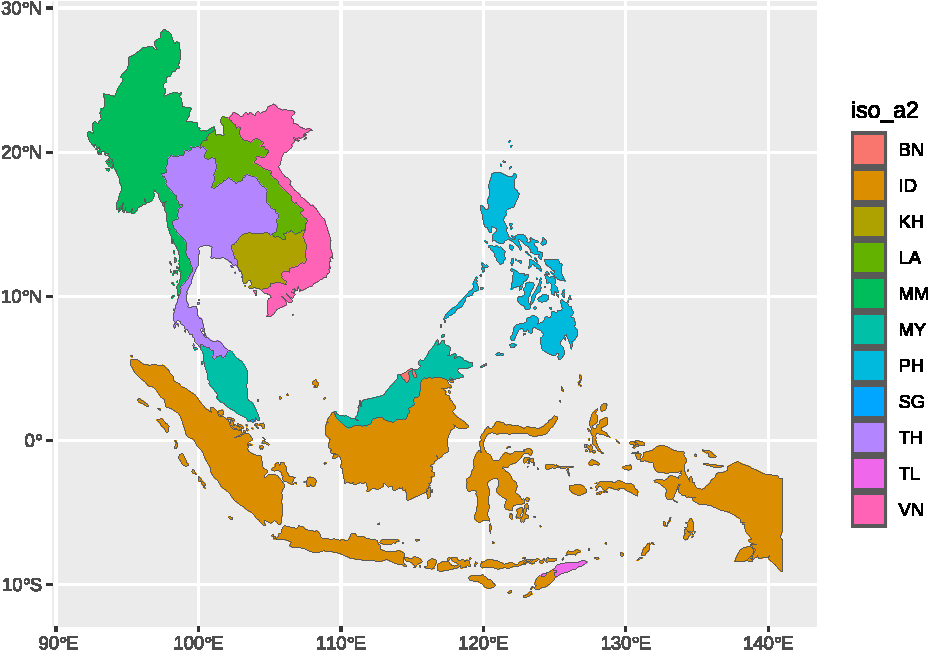
\includegraphics{03-first-example_files/figure-latex/unnamed-chunk-16-1.pdf}

これらは、世界全体の GPT における割合です。

どのようなことがわかりますか。

主要国で、60\%〜70\% を占めていることがわかります。それぞれの国や、幾つかの国の影響力も、ある程度みることができるように見えます。

気づいたこと、疑問に思ったことなどを、書き出してみてください。

GDP が大きな国と、小さな国があるのはわかりますが、それは、どのように分布しているのでしょうか。

\hypertarget{fig-5.-2021ux5e74ux306eux4e16ux754cux306eux56fdux306egdpux306eux5206ux5e03uxff11}{%
\subsubsection{Fig 5. 2021年の世界の国のGDPの分布(1)}\label{fig-5.-2021ux5e74ux306eux4e16ux754cux306eux56fdux306egdpux306eux5206ux5e03uxff11}}

\begin{Shaded}
\begin{Highlighting}[]
\NormalTok{df\_gdp }\SpecialCharTok{\%\textgreater{}\%} \FunctionTok{drop\_na}\NormalTok{(gdp) }\SpecialCharTok{\%\textgreater{}\%} 
  \FunctionTok{filter}\NormalTok{(year }\SpecialCharTok{==} \DecValTok{2021}\NormalTok{) }\SpecialCharTok{\%\textgreater{}\%} \FunctionTok{filter}\NormalTok{(region }\SpecialCharTok{!=} \StringTok{"Aggregates"}\NormalTok{) }\SpecialCharTok{\%\textgreater{}\%}
  \FunctionTok{ggplot}\NormalTok{(}\FunctionTok{aes}\NormalTok{(gdp)) }\SpecialCharTok{+} \FunctionTok{geom\_histogram}\NormalTok{()}
\CommentTok{\#\textgreater{} \textasciigrave{}stat\_bin()\textasciigrave{} using \textasciigrave{}bins = 30\textasciigrave{}. Pick better value with}
\CommentTok{\#\textgreater{} \textasciigrave{}binwidth\textasciigrave{}.}
\end{Highlighting}
\end{Shaded}

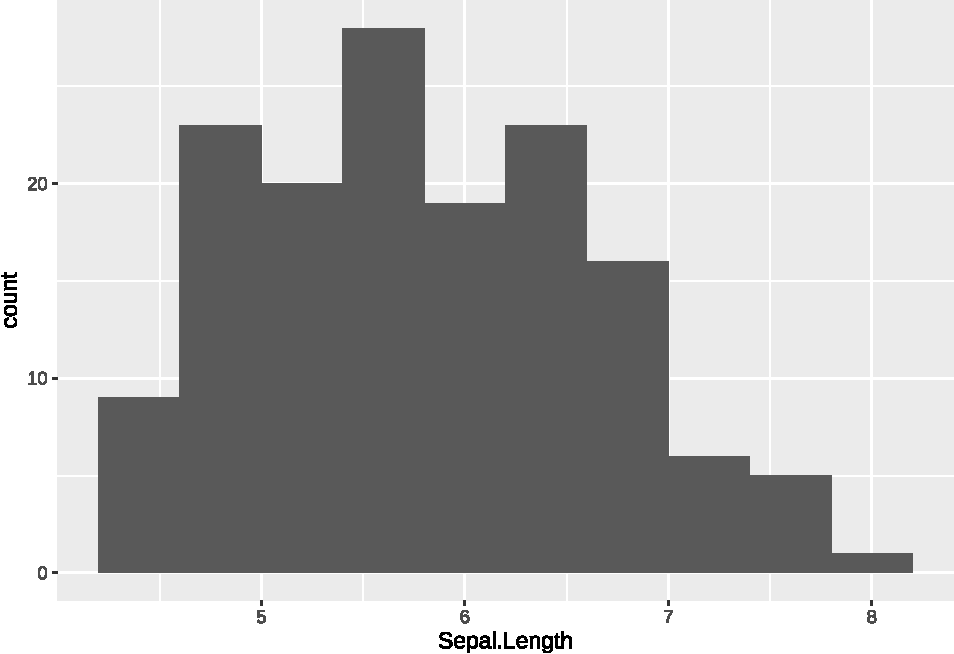
\includegraphics{03-first-example_files/figure-latex/unnamed-chunk-17-1.pdf}

小さいところに集中していることがわかりますが、\texttt{scale\_x\_log10()} を加え、対数軸をとってみます。

\(log10(1000) = 3\), \(log10(1000000) = 6\), \(log10(1000000000) = 9\) などになります。

\hypertarget{fig-6.-2021ux5e74ux306eux4e16ux754cux306eux56fdux306egdpux306eux5206ux5e03uxff12}{%
\subsubsection{Fig 6. 2021年の世界の国のGDPの分布(2)}\label{fig-6.-2021ux5e74ux306eux4e16ux754cux306eux56fdux306egdpux306eux5206ux5e03uxff12}}

\begin{Shaded}
\begin{Highlighting}[]
\NormalTok{df\_gdp }\SpecialCharTok{\%\textgreater{}\%} \FunctionTok{drop\_na}\NormalTok{(gdp) }\SpecialCharTok{\%\textgreater{}\%} 
  \FunctionTok{filter}\NormalTok{(year }\SpecialCharTok{==} \DecValTok{2021}\NormalTok{) }\SpecialCharTok{\%\textgreater{}\%} \FunctionTok{filter}\NormalTok{(region }\SpecialCharTok{!=} \StringTok{"Aggregates"}\NormalTok{) }\SpecialCharTok{\%\textgreater{}\%}
  \FunctionTok{ggplot}\NormalTok{(}\FunctionTok{aes}\NormalTok{(gdp)) }\SpecialCharTok{+} \FunctionTok{geom\_histogram}\NormalTok{() }\SpecialCharTok{+} \FunctionTok{scale\_x\_log10}\NormalTok{()}
\CommentTok{\#\textgreater{} \textasciigrave{}stat\_bin()\textasciigrave{} using \textasciigrave{}bins = 30\textasciigrave{}. Pick better value with}
\CommentTok{\#\textgreater{} \textasciigrave{}binwidth\textasciigrave{}.}
\end{Highlighting}
\end{Shaded}

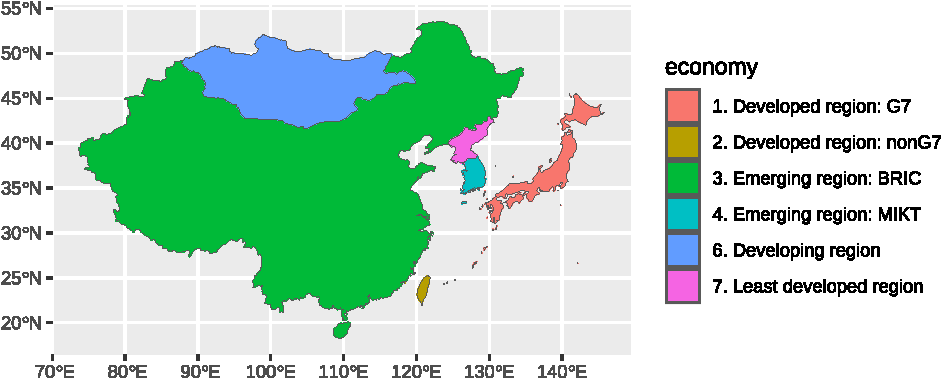
\includegraphics{03-first-example_files/figure-latex/unnamed-chunk-18-1.pdf}

幅を変更したり、分ける個数を変更するには \texttt{binwidth\ =\ 0.5} や、\texttt{bins\ =\ 20} を、\texttt{geom\_histogram()} のかっこの中に入れます。

\hypertarget{fig-7.-2021ux5e74ux306eux4e16ux754cux306eux56fdux306egdpux306eux5206ux5e03uxff13}{%
\subsubsection{Fig 7. 2021年の世界の国のGDPの分布(3)}\label{fig-7.-2021ux5e74ux306eux4e16ux754cux306eux56fdux306egdpux306eux5206ux5e03uxff13}}

また、密度曲線に変えるには、\texttt{geom\_density} を使います。

\begin{Shaded}
\begin{Highlighting}[]
\NormalTok{df\_gdp }\SpecialCharTok{\%\textgreater{}\%} \FunctionTok{drop\_na}\NormalTok{(gdp) }\SpecialCharTok{\%\textgreater{}\%} 
  \FunctionTok{filter}\NormalTok{(year }\SpecialCharTok{==} \DecValTok{2021}\NormalTok{) }\SpecialCharTok{\%\textgreater{}\%} \FunctionTok{filter}\NormalTok{(region }\SpecialCharTok{!=} \StringTok{"Aggregates"}\NormalTok{) }\SpecialCharTok{\%\textgreater{}\%}
  \FunctionTok{ggplot}\NormalTok{(}\FunctionTok{aes}\NormalTok{(gdp)) }\SpecialCharTok{+} \FunctionTok{geom\_density}\NormalTok{() }\SpecialCharTok{+} \FunctionTok{scale\_x\_log10}\NormalTok{()}
\end{Highlighting}
\end{Shaded}

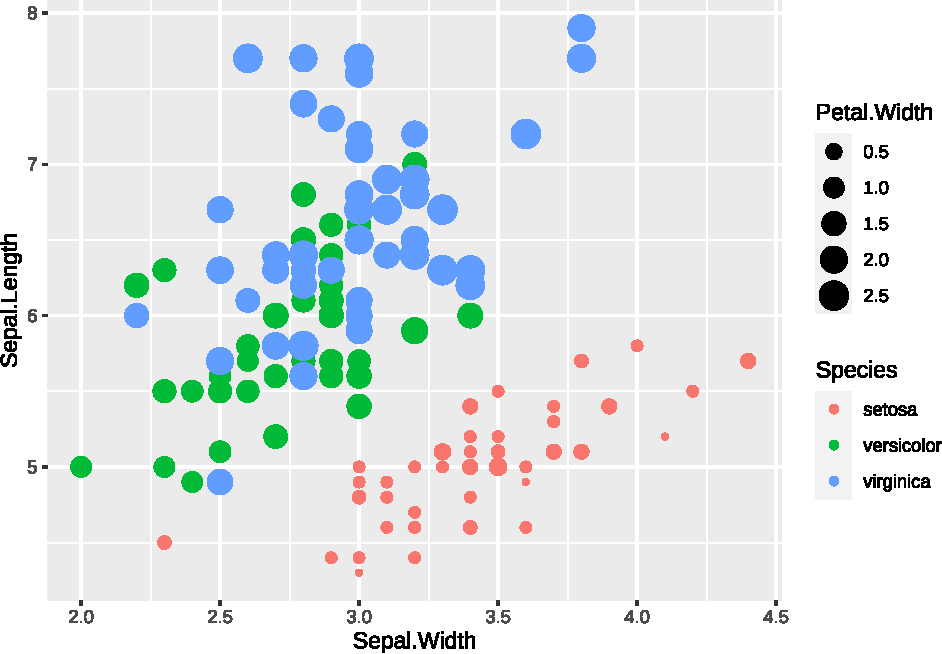
\includegraphics{03-first-example_files/figure-latex/unnamed-chunk-19-1.pdf}

\hypertarget{fig-8.-2021ux5e74ux306eux4e16ux754cux306eux56fdux306egdpux306eux5206ux5e03uxff14}{%
\subsubsection{Fig 8. 2021年の世界の国のGDPの分布(4)}\label{fig-8.-2021ux5e74ux306eux4e16ux754cux306eux56fdux306egdpux306eux5206ux5e03uxff14}}

これは、2021年のデータですが、density の変化を見てみます。alpha の値は透明度です。

\begin{Shaded}
\begin{Highlighting}[]
\NormalTok{df\_gdp }\SpecialCharTok{\%\textgreater{}\%} \FunctionTok{drop\_na}\NormalTok{(gdp) }\SpecialCharTok{\%\textgreater{}\%} 
  \FunctionTok{filter}\NormalTok{(year }\SpecialCharTok{\%in\%} \FunctionTok{c}\NormalTok{(}\DecValTok{1961}\NormalTok{, }\DecValTok{1971}\NormalTok{, }\DecValTok{1981}\NormalTok{, }\DecValTok{1991}\NormalTok{, }\DecValTok{2001}\NormalTok{, }\DecValTok{2011}\NormalTok{, }\DecValTok{2021}\NormalTok{)) }\SpecialCharTok{\%\textgreater{}\%}
  \FunctionTok{ggplot}\NormalTok{(}\FunctionTok{aes}\NormalTok{(gdp, }\AttributeTok{fill =} \FunctionTok{factor}\NormalTok{(year))) }\SpecialCharTok{+} \FunctionTok{geom\_density}\NormalTok{(}\AttributeTok{alpha =} \FloatTok{0.4}\NormalTok{) }\SpecialCharTok{+} \FunctionTok{scale\_x\_log10}\NormalTok{()}
\end{Highlighting}
\end{Shaded}

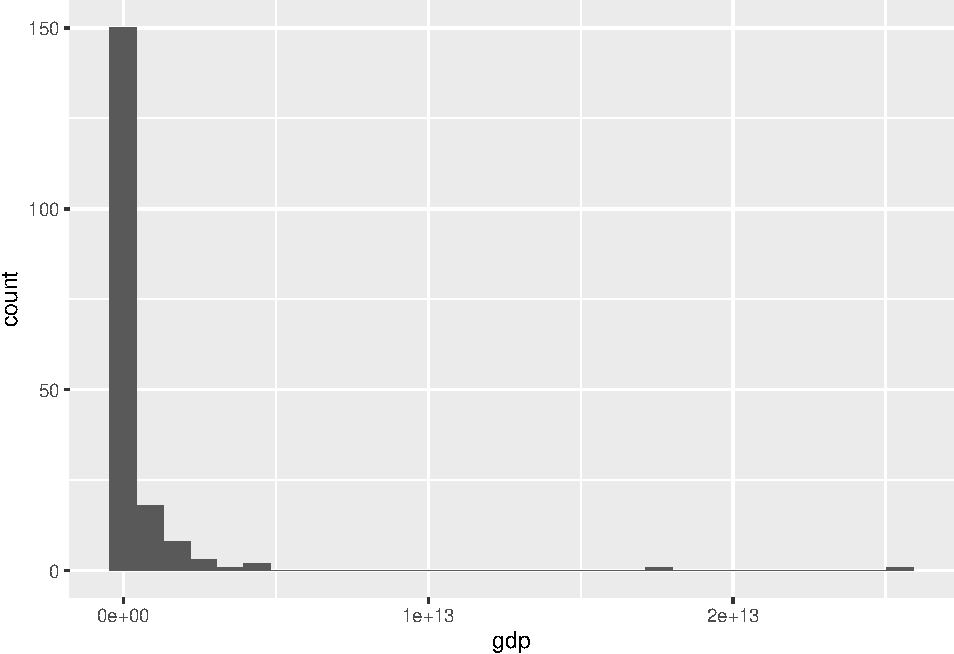
\includegraphics{03-first-example_files/figure-latex/unnamed-chunk-20-1.pdf}

\hypertarget{fig-9.-2021ux5e74ux306eux4e16ux754cux306eux56fdux306egdpux306eux5206ux5e03uxff15}{%
\subsubsection{Fig 9. 2021年の世界の国のGDPの分布(5)}\label{fig-9.-2021ux5e74ux306eux4e16ux754cux306eux56fdux306egdpux306eux5206ux5e03uxff15}}

少しみにくいので、分けてみます。

\begin{Shaded}
\begin{Highlighting}[]
\NormalTok{df\_gdp }\SpecialCharTok{\%\textgreater{}\%} \FunctionTok{drop\_na}\NormalTok{(gdp) }\SpecialCharTok{\%\textgreater{}\%} 
  \FunctionTok{filter}\NormalTok{(year }\SpecialCharTok{\%in\%} \FunctionTok{c}\NormalTok{(}\DecValTok{1971}\NormalTok{, }\DecValTok{1981}\NormalTok{, }\DecValTok{1991}\NormalTok{, }\DecValTok{2001}\NormalTok{, }\DecValTok{2011}\NormalTok{, }\DecValTok{2021}\NormalTok{)) }\SpecialCharTok{\%\textgreater{}\%}
  \FunctionTok{ggplot}\NormalTok{(}\FunctionTok{aes}\NormalTok{(gdp, }\AttributeTok{fill =} \FunctionTok{factor}\NormalTok{(year))) }\SpecialCharTok{+} 
  \FunctionTok{geom\_density}\NormalTok{() }\SpecialCharTok{+} \FunctionTok{scale\_x\_log10}\NormalTok{() }\SpecialCharTok{+} \FunctionTok{facet\_wrap}\NormalTok{(}\SpecialCharTok{\textasciitilde{}}\NormalTok{year)}
\end{Highlighting}
\end{Shaded}

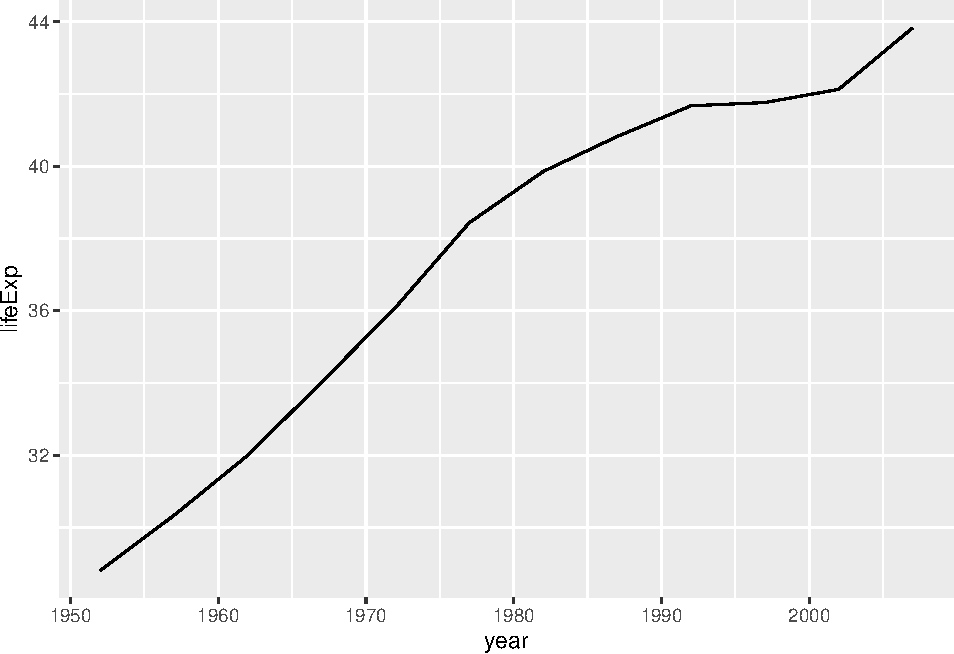
\includegraphics{03-first-example_files/figure-latex/unnamed-chunk-21-1.pdf}

\hypertarget{fig-10.-ux5730ux57dfux3054ux3068ux306e-gdp-ux306eux5206ux5e03}{%
\subsubsection{Fig 10. 地域ごとの GDP の分布}\label{fig-10.-ux5730ux57dfux3054ux3068ux306e-gdp-ux306eux5206ux5e03}}

いくつかのグループごとに分布をみてみることも可能です。それには、Boxplot が有効です。

\begin{Shaded}
\begin{Highlighting}[]
\NormalTok{df\_gdp }\SpecialCharTok{\%\textgreater{}\%} \FunctionTok{drop\_na}\NormalTok{(gdp) }\SpecialCharTok{\%\textgreater{}\%} \FunctionTok{filter}\NormalTok{(region }\SpecialCharTok{!=} \StringTok{"Aggregates"}\NormalTok{) }\SpecialCharTok{\%\textgreater{}\%}
  \FunctionTok{drop\_na}\NormalTok{(region) }\SpecialCharTok{\%\textgreater{}\%} \FunctionTok{filter}\NormalTok{(year }\SpecialCharTok{\%in\%} \FunctionTok{c}\NormalTok{(}\DecValTok{2021}\NormalTok{)) }\SpecialCharTok{\%\textgreater{}\%}
  \FunctionTok{ggplot}\NormalTok{(}\FunctionTok{aes}\NormalTok{(gdp, region, }\AttributeTok{fill =}\NormalTok{ region)) }\SpecialCharTok{+} 
  \FunctionTok{geom\_boxplot}\NormalTok{() }\SpecialCharTok{+} \FunctionTok{scale\_x\_log10}\NormalTok{() }\SpecialCharTok{+} \FunctionTok{labs}\NormalTok{(}\AttributeTok{y =} \StringTok{""}\NormalTok{) }\SpecialCharTok{+} 
  \FunctionTok{theme}\NormalTok{(}\AttributeTok{legend.position =} \StringTok{"none"}\NormalTok{)}
\end{Highlighting}
\end{Shaded}

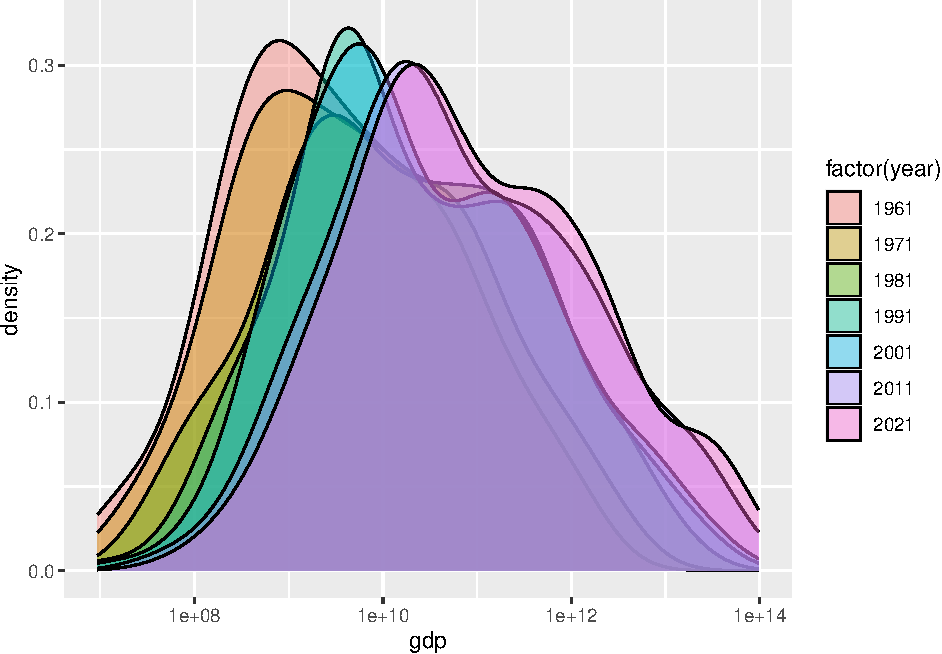
\includegraphics{03-first-example_files/figure-latex/unnamed-chunk-22-1.pdf}

\hypertarget{fig-11.-ux53ceux5165ux306eux591aux5be1ux306bux3088ux308bux5206ux985eux3054ux3068ux306e-gdp-ux5206ux5e03}{%
\subsubsection{Fig 11. 収入の多寡による分類ごとの GDP 分布}\label{fig-11.-ux53ceux5165ux306eux591aux5be1ux306bux3088ux308bux5206ux985eux3054ux3068ux306e-gdp-ux5206ux5e03}}

\begin{Shaded}
\begin{Highlighting}[]
\NormalTok{df\_gdp }\SpecialCharTok{\%\textgreater{}\%} \FunctionTok{drop\_na}\NormalTok{(gdp) }\SpecialCharTok{\%\textgreater{}\%} \FunctionTok{filter}\NormalTok{(region }\SpecialCharTok{!=} \StringTok{"Aggregates"}\NormalTok{) }\SpecialCharTok{\%\textgreater{}\%}
  \FunctionTok{drop\_na}\NormalTok{(income) }\SpecialCharTok{\%\textgreater{}\%} \FunctionTok{filter}\NormalTok{(year }\SpecialCharTok{\%in\%} \FunctionTok{c}\NormalTok{(}\DecValTok{2021}\NormalTok{)) }\SpecialCharTok{\%\textgreater{}\%}
  \FunctionTok{mutate}\NormalTok{(}\AttributeTok{level =} \FunctionTok{factor}\NormalTok{(income, }\FunctionTok{c}\NormalTok{(}\StringTok{"High income"}\NormalTok{, }\StringTok{"Upper middle income"}\NormalTok{, }\StringTok{"Lower middle income"}\NormalTok{, }\StringTok{"Low income"}\NormalTok{))) }\SpecialCharTok{\%\textgreater{}\%}
  \FunctionTok{ggplot}\NormalTok{(}\FunctionTok{aes}\NormalTok{(gdp, level, }\AttributeTok{fill =}\NormalTok{ income)) }\SpecialCharTok{+} 
  \FunctionTok{geom\_boxplot}\NormalTok{() }\SpecialCharTok{+} \FunctionTok{scale\_x\_log10}\NormalTok{() }\SpecialCharTok{+} \FunctionTok{labs}\NormalTok{(}\AttributeTok{y =} \StringTok{""}\NormalTok{) }\SpecialCharTok{+} 
  \FunctionTok{theme}\NormalTok{(}\AttributeTok{legend.position =} \StringTok{"none"}\NormalTok{)}
\end{Highlighting}
\end{Shaded}

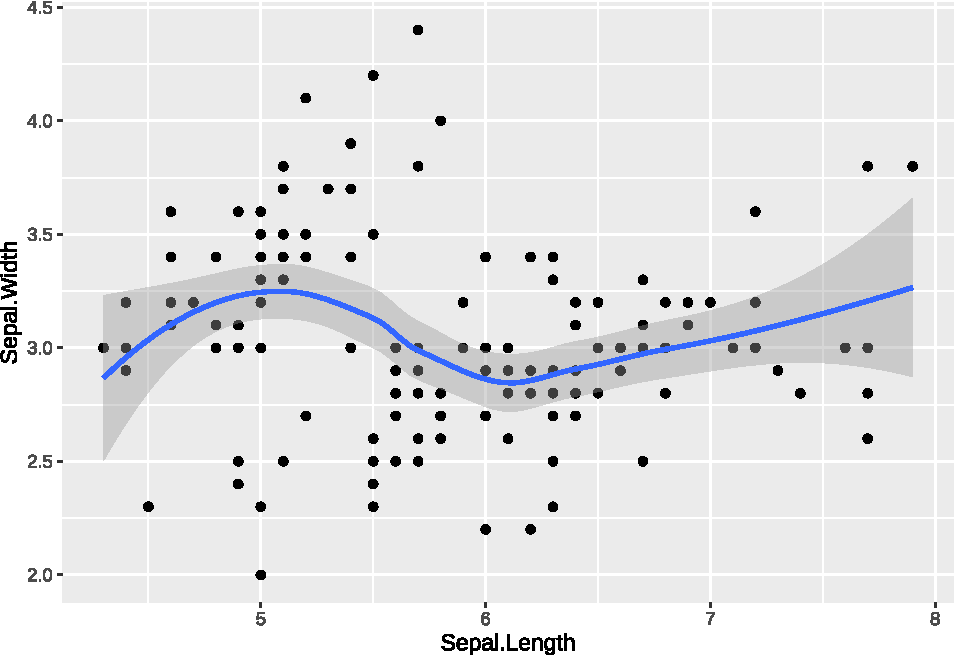
\includegraphics{03-first-example_files/figure-latex/unnamed-chunk-23-1.pdf}

これからも、いろいろなことがわかりますね。

\hypertarget{ux4e16ux754cux5730ux56f3ux306eux6e96ux5099}{%
\subsubsection{世界地図の準備}\label{ux4e16ux754cux5730ux56f3ux306eux6e96ux5099}}

地図で、国の income level をみてみましょう。

\begin{Shaded}
\begin{Highlighting}[]
\FunctionTok{library}\NormalTok{(maps)}
\NormalTok{gdp\_short }\OtherTok{\textless{}{-}}\NormalTok{ df\_gdp }\SpecialCharTok{\%\textgreater{}\%} \FunctionTok{filter}\NormalTok{(year }\SpecialCharTok{==} \DecValTok{2021}\NormalTok{, region }\SpecialCharTok{!=} \StringTok{"Aggregates"}\NormalTok{) }\SpecialCharTok{\%\textgreater{}\%}
  \FunctionTok{select}\NormalTok{(iso2c, gdp, income)}
\NormalTok{map\_world }\OtherTok{\textless{}{-}} \FunctionTok{map\_data}\NormalTok{(}\StringTok{\textquotesingle{}world\textquotesingle{}}\NormalTok{)}
\NormalTok{map\_gdp }\OtherTok{\textless{}{-}}\NormalTok{ map\_world }\SpecialCharTok{\%\textgreater{}\%} 
  \FunctionTok{mutate}\NormalTok{(}\AttributeTok{iso2c =} \FunctionTok{iso.alpha}\NormalTok{(region, }\AttributeTok{n=}\DecValTok{2}\NormalTok{)) }\SpecialCharTok{\%\textgreater{}\%} 
  \FunctionTok{left\_join}\NormalTok{(gdp\_short, }\AttributeTok{by =} \StringTok{"iso2c"}\NormalTok{) }
\FunctionTok{head}\NormalTok{(map\_gdp)}
\CommentTok{\#\textgreater{}        long      lat group order region subregion iso2c}
\CommentTok{\#\textgreater{} 1 {-}69.89912 12.45200     1     1  Aruba      \textless{}NA\textgreater{}    AW}
\CommentTok{\#\textgreater{} 2 {-}69.89571 12.42300     1     2  Aruba      \textless{}NA\textgreater{}    AW}
\CommentTok{\#\textgreater{} 3 {-}69.94219 12.43853     1     3  Aruba      \textless{}NA\textgreater{}    AW}
\CommentTok{\#\textgreater{} 4 {-}70.00415 12.50049     1     4  Aruba      \textless{}NA\textgreater{}    AW}
\CommentTok{\#\textgreater{} 5 {-}70.06612 12.54697     1     5  Aruba      \textless{}NA\textgreater{}    AW}
\CommentTok{\#\textgreater{} 6 {-}70.05088 12.59707     1     6  Aruba      \textless{}NA\textgreater{}    AW}
\CommentTok{\#\textgreater{}          gdp      income}
\CommentTok{\#\textgreater{} 1 3126019385 High income}
\CommentTok{\#\textgreater{} 2 3126019385 High income}
\CommentTok{\#\textgreater{} 3 3126019385 High income}
\CommentTok{\#\textgreater{} 4 3126019385 High income}
\CommentTok{\#\textgreater{} 5 3126019385 High income}
\CommentTok{\#\textgreater{} 6 3126019385 High income}
\end{Highlighting}
\end{Shaded}

\hypertarget{fig-12.-income-level-ux306bux3088ux308bux8272ux5206ux3051ux5730ux56f3}{%
\subsubsection{Fig 12. Income Level による色分け地図}\label{fig-12.-income-level-ux306bux3088ux308bux8272ux5206ux3051ux5730ux56f3}}

\begin{Shaded}
\begin{Highlighting}[]
\NormalTok{map\_gdp }\SpecialCharTok{\%\textgreater{}\%} \FunctionTok{mutate}\NormalTok{(}\AttributeTok{income\_level =} \FunctionTok{factor}\NormalTok{(income, }\AttributeTok{levels =} \FunctionTok{c}\NormalTok{(}\StringTok{"High income"}\NormalTok{, }\StringTok{"Upper middle income"}\NormalTok{, }\StringTok{"Lower middle income"}\NormalTok{, }\StringTok{"Low income"}\NormalTok{, }\StringTok{"Not classified"}\NormalTok{, }\ConstantTok{NA}\NormalTok{))) }\SpecialCharTok{\%\textgreater{}\%}
  \FunctionTok{ggplot}\NormalTok{() }\SpecialCharTok{+}
  \FunctionTok{geom\_map}\NormalTok{(}\FunctionTok{aes}\NormalTok{(long, lat, }\AttributeTok{map\_id =}\NormalTok{ region, }\AttributeTok{fill =}\NormalTok{ income\_level), }\AttributeTok{map =}\NormalTok{ map\_world, }\AttributeTok{col =} \StringTok{"black"}\NormalTok{, }\AttributeTok{size =} \FloatTok{0.1}\NormalTok{) }
\CommentTok{\#\textgreater{} Warning: Using \textasciigrave{}size\textasciigrave{} aesthetic for lines was deprecated in ggplot2}
\CommentTok{\#\textgreater{} 3.4.0.}
\CommentTok{\#\textgreater{} i Please use \textasciigrave{}linewidth\textasciigrave{} instead.}
\CommentTok{\#\textgreater{} This warning is displayed once every 8 hours.}
\CommentTok{\#\textgreater{} Call \textasciigrave{}lifecycle::last\_lifecycle\_warnings()\textasciigrave{} to see where}
\CommentTok{\#\textgreater{} this warning was generated.}
\CommentTok{\#\textgreater{} Warning in geom\_map(aes(long, lat, map\_id = region, fill =}
\CommentTok{\#\textgreater{} income\_level), : Ignoring unknown aesthetics: x and y}
\end{Highlighting}
\end{Shaded}

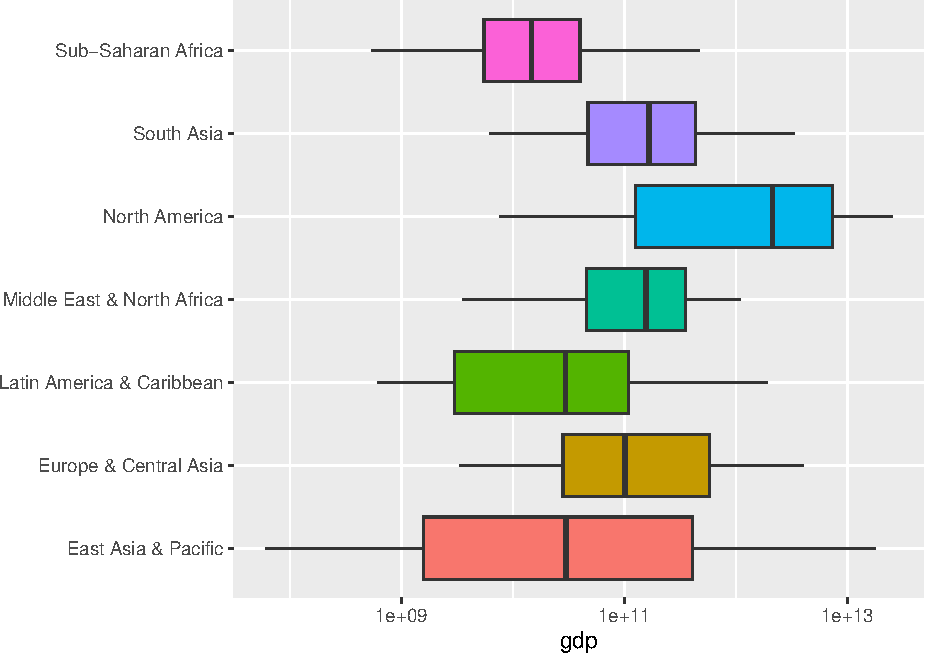
\includegraphics{03-first-example_files/figure-latex/unnamed-chunk-25-1.pdf}

\hypertarget{fig-13.-gdp-ux306bux3088ux308bux8272ux5206ux3051ux5730ux56f3}{%
\subsubsection{Fig 13. GDP による色分け地図}\label{fig-13.-gdp-ux306bux3088ux308bux8272ux5206ux3051ux5730ux56f3}}

\begin{Shaded}
\begin{Highlighting}[]
\NormalTok{map\_gdp }\SpecialCharTok{\%\textgreater{}\%}
  \FunctionTok{ggplot}\NormalTok{() }\SpecialCharTok{+}
  \FunctionTok{geom\_map}\NormalTok{(}\FunctionTok{aes}\NormalTok{(}\AttributeTok{x=}\NormalTok{long, }\AttributeTok{y=}\NormalTok{lat, }\AttributeTok{map\_id =}\NormalTok{ region, }\AttributeTok{fill =}\NormalTok{ gdp), }\AttributeTok{map =}\NormalTok{ map\_world, }\AttributeTok{col =} \StringTok{"black"}\NormalTok{, }\AttributeTok{size =} \FloatTok{0.1}\NormalTok{) }
\CommentTok{\#\textgreater{} Warning in geom\_map(aes(x = long, y = lat, map\_id = region,}
\CommentTok{\#\textgreater{} fill = gdp), : Ignoring unknown aesthetics: x and y}
\end{Highlighting}
\end{Shaded}

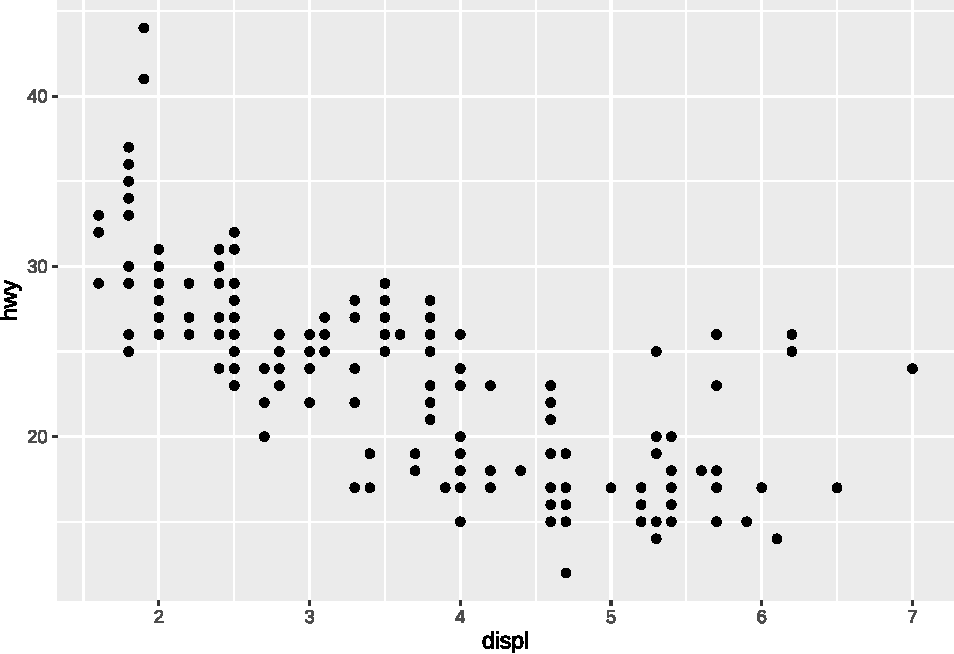
\includegraphics{03-first-example_files/figure-latex/unnamed-chunk-26-1.pdf}

\hypertarget{ux7df4ux7fd2}{%
\section{練習}\label{ux7df4ux7fd2}}

\begin{enumerate}
\def\labelenumi{\arabic{enumi}.}
\tightlist
\item
  それぞれのグラフから、わかったこと、問いなどを列挙してみましょう。
\item
  Fig 1 の Japan の部分を他の国や、グループ(World など)に変えてみてください。何がわかりますか。
\item
  Fig 3 の iso2c で選択する、国を変更してください。何がわかりますか。
\item
  Fig 4 または Fig 5 の iso2c の部分を他の国に変更してください。何がわかりますか。
\item
  Fig 5 または Fig 6 の、区間の幅や、数を 変更してみてください。何がわかりますか。
\item
  Fig 7, Fig 8, Fig 9 の年を変更してみてください。何がわかりますか。
\item
  Fig 12, Fig 13 の年を変更してみてください。何がわかりますか。
\end{enumerate}

\hypertarget{ux30d7ux30edux30b8ux30a7ux30afux30c8}{%
\section{プロジェクト}\label{ux30d7ux30edux30b8ux30a7ux30afux30c8}}

他のデータで、同様のことをしてみましょう。

\begin{enumerate}
\def\labelenumi{\arabic{enumi}.}
\tightlist
\item
  最初に、\texttt{gdp\ =\ "NY.GDP.MKTP.CD"} としましたが、GNI per capita, Atlas method (current US\$): NY.GNP.PCAP.CD に変えてみましょう。
\end{enumerate}

\begin{Shaded}
\begin{Highlighting}[]
\NormalTok{df\_gnppcap }\OtherTok{\textless{}{-}} \FunctionTok{WDI}\NormalTok{(}\AttributeTok{country =} \StringTok{"all"}\NormalTok{, }
              \AttributeTok{indicator =} \FunctionTok{c}\NormalTok{(}\AttributeTok{gnppcap =} \StringTok{"NY.GNP.PCAP.CD"}\NormalTok{), }
              \AttributeTok{extra =} \ConstantTok{TRUE}\NormalTok{)}
\end{Highlighting}
\end{Shaded}

\begin{enumerate}
\def\labelenumi{\arabic{enumi}.}
\setcounter{enumi}{1}
\tightlist
\item
  \href{https://datatopics.worldbank.org/world-development-indicators/}{World Development Indicators} のサイトの下にある、Data Themes(テーマ)から自分が調べたいテーマを選び、そのテーマから、データコードを取得して、同様の分析をしてみてください。データがあまりない場合もありますので、ある程度データが多いものを選択することをお勧めします。
\end{enumerate}

\hypertarget{ux307eux3068ux3081}{%
\section{まとめ}\label{ux307eux3068ux3081}}

今回は、経済指標である、GDP を使いました。データサイエンスについて少しずつ、学んでいきます。

コードの説明は、簡単にしかしていませんから、理解するのは難しいと思いますが、いくつかのことは、ご理解いただけると思います。

\begin{itemize}
\item
  それほど、長くはない、コードで、データを見ていく。R は対話型(interactive)のプログラミング言語と言われています。
\item
  コードに続けて、結果が表示されるので、コードと出力の対応が見やすい。また、コメントや説明も併記することができる。これは、RMarkdown という形式の中で、コードを書いていることによるものです。RMarkdown は、再現性(reproducibility)と、プログラム・コードの内容をコンピュータにわかるようにでなく、人間にもわかるように記述する(Literate Programming)を実現しています。
\item
  視覚化(Visualization)によって、わかることが色々とある。また、視覚化の方法もたくさんあり、いろいろな見方をすることで、データについての理解が深まっていく。
\item
  視覚化を通して、データを理解すること、問いを持ち、他の視覚化などを用いて、さらに、理解を深めることがたいせつ。
\item
  理解したことを元にして、さらに、そのデータ、または、他のデータを使って、新たな発見をしていく。
\end{itemize}

統計的な指標も用いますが、それらによって、新しい知識を生み出すとも表現しますが、そのような営み全体が、データサイエンスの核をなす部分だと思います。

\hypertarget{wdi-site}{%
\chapter{世界開発指標}\label{wdi-site}}

世界銀行(World Bank)の 世界開発指標(WDI)の中の、GDP を使いました。どのようなものか確認しておきましょう。

\hypertarget{ux4e16ux754cux9280ux884cworld-bank}{%
\section{\texorpdfstring{世界銀行(\href{https://www.worldbank.org/en/home}{World Bank})}{世界銀行(World Bank)}}\label{ux4e16ux754cux9280ux884cworld-bank}}

\begin{itemize}
\tightlist
\item
  \href{https://data.worldbank.org}{世界銀行オープンデータ}
\item
  \href{https://datacatalog.worldbank.org/home}{データカタログ}
\item
  \href{https://datatopics.worldbank.org/world-development-indicators/}{世界開発指標(WDI)}
\end{itemize}

世界開発指標は、世界銀行が提供している、オープンデータの一つで、他にも、たくさんのデータを提供しています。三つのサイトのリンクを書きました。一つ一つみていきましょう。

まず、英語を読むことが苦手な場合は、ブラウザー(Google Chrome, Edge, Safari などのホームページ閲覧ソフト)の自動翻訳機能を使うのも良いでしょう。しかし、自動翻訳機能を利用していると、リンク先に飛べなかったり、いくつかの機能が使えないこともありますので、ボタンを押しても、反応しないときは、自動翻訳機能を OFF にして利用してください。

\hypertarget{ux4e16ux754cux9280ux884cux30aaux30fcux30d7ux30f3ux30c7ux30fcux30bf}{%
\subsection{\texorpdfstring{\href{https://data.worldbank.org}{世界銀行オープンデータ}}{世界銀行オープンデータ}}\label{ux4e16ux754cux9280ux884cux30aaux30fcux30d7ux30f3ux30c7ux30fcux30bf}}

上の検索窓の下に、Country と Indicators と書いてあります。

\hypertarget{ux56fdux5225ux30b5ux30a4ux30c8}{%
\subsubsection{国別サイト}\label{ux56fdux5225ux30b5ux30a4ux30c8}}

Country(国別)のサイトを選択すると、国のリストが出てきます。

J のところに、Japan(日本)がありますから、選択すると、日本のさまざまな指標とグラフが出てきます。

Indicator(指標)、Most Recent Values(直近の値)、Trend(傾向)が表示されます。指標をクリックすると、大きなグラフが出てきます。その指標のサイトですから、そこで、その指標についての他の国の状況などを確認することができます。そこでは、選択した指標と似た指標が選択できたり、もっと詳しいことをしらべるデータバンクへのリンクもあります。このサイトから、データをダウンロードすることもできるようになっています。

また、国別サイトを開けると、右の方には、地域など、グループに分けてある箇所もあります。その一番下には、World (世界)もありますから、世界全体について見てみたり、収入の階級に分けたサイトの指標を見ることもできるようになっています。

\hypertarget{ux6307ux6a19ux5225ux30b5ux30a4ux30c8}{%
\subsubsection{指標別サイト}\label{ux6307ux6a19ux5225ux30b5ux30a4ux30c8}}

Indicators(指標)を選択すると、トピックに分けて、指標が並んでいます。

よく見ると、一番上に、Featured Indicators(特徴的な指標) と、All Indicators(すべての指標) となっていて、最初の開いているのは、特徴的な指標の方であることがわかります。すべての指標の方を開けると、たくさんの指標を見ることができます。

トピックは、以下のものに分かれています。

\begin{itemize}
\tightlist
\item
  Agriculture \& Rural Development 農業と農村開発
\item
  Aid Effectiveness 援助の有効性
\item
  Climate Change 気候変動
\item
  Economy \& Growth 経済と成長
\item
  Education 教育
\item
  Energy \& Mining エネルギーと鉱業
\item
  Environment 環境
\item
  External Debt 対外債務
\item
  Financial Sector 金融セクター
\item
  Gender 性別
\item
  Health 健康
\item
  Infrastructure インフラ
\item
  Poverty 貧困
\item
  Private Sector 民間部門
\item
  Public Sector 公共部門
\item
  Science \& Technology 科学技術
\item
  Social Development 社会開発
\item
  Social Protection \& Labor 社会的保護と労働
\item
  Trade 貿易
\item
  Urban Development 都市開発
\end{itemize}

それぞれの指標を選択すると、グラフが表示される画面が出てきます。それは、上で国別のところから選択したものと同じです。

Indicator Code (WDI コード)は、Details (詳細) を見ると、その指標の概要とともに、書いてあります。 そのデータコードは、そのページの上の URL にも表示されています。

\hypertarget{ux30c7ux30fcux30bfux30abux30bfux30edux30b0}{%
\subsection{\texorpdfstring{\href{https://datacatalog.worldbank.org/home}{データカタログ}}{データカタログ}}\label{ux30c7ux30fcux30bfux30abux30bfux30edux30b0}}

\hypertarget{ux4e16ux754cux958bux767aux6307ux6a19wdi}{%
\subsection{\texorpdfstring{\href{https://datatopics.worldbank.org/world-development-indicators/}{世界開発指標(WDI)}}{世界開発指標(WDI)}}\label{ux4e16ux754cux958bux767aux6307ux6a19wdi}}

また、オープンデータについて、世界銀行は、厳密な定義をしています。

\hypertarget{ux30aaux30fcux30d7ux30f3ux30c7ux30fcux30bfux306eux5b9aux7fa9open-data-defined}{%
\subsection{\texorpdfstring{オープンデータの定義(\href{http://opendatatoolkit.worldbank.org/en/essentials.html}{Open Data Defined})}{オープンデータの定義(Open Data Defined)}}\label{ux30aaux30fcux30d7ux30f3ux30c7ux30fcux30bfux306eux5b9aux7fa9open-data-defined}}

オープンデータという言葉は、厳密な意味を持っています。データまたはコンテンツは、出所が明示されオープンという性質が維持されれば、誰でも自由に利用、再利用、再配布できるものを言います。

\begin{enumerate}
\def\labelenumi{\arabic{enumi}.}
\item
  データは法的にオープンでなければなりません。つまり、パブリックドメインに置かれ、最小限の制限で自由に使用できなければなりません。
\item
  データは技術的にオープンでなければなりません。つまり、誰でも自由に使える一般的なソフトウェアツールを使ってデータにアクセスし、機械で読み取ることが可読な電子フォーマットで提供されていなければならなりません。パスワードやファイアウォールによる制限を受けずに、公共のサーバーで、だれでもアクセスできなければなりません。また、オープンデータを見つけやすくするために、さまざまな組織がオープンデータカタログを作成し管理してく必要があります。
\end{enumerate}

データはだれのものでしょうか? パブリックデータのパブリックとは?

\hypertarget{ux4e16ux754cux958bux767aux6307ux6a19wdi-1}{%
\section{世界開発指標(WDI)}\label{ux4e16ux754cux958bux767aux6307ux6a19wdi-1}}

\begin{itemize}
\tightlist
\item
  \href{https://datatopics.worldbank.org/world-development-indicators/}{World Development Indicators (WDI)} : 世界銀行が開発に関する各国間比較可能なデータの集大成である1400の時系列指標(the World Bank's premier compilation of cross-country comparable data on development; 1400 time series indicators)

  \begin{itemize}
  \tightlist
  \item
    テーマ別(Themes): 貧困と格差、人間、環境、経済、国家と市場、グローバルリンク集(Poverty and Inequality, People, Environment, Economy, States and Markets, Global Links)
  \item
    オープンデータとデータバンク(Open Data \& DataBank): Explore data, Query database
  \item
    Bulk Download: Excel, CSV
  \item
    API Documentation
  \end{itemize}
\end{itemize}

\hypertarget{ux4e16ux754cux306eux3055ux307eux3056ux307eux306aux8ab2ux984c}{%
\subsection{世界のさまざまな課題}\label{ux4e16ux754cux306eux3055ux307eux3056ux307eux306aux8ab2ux984c}}

\url{https://datatopics.worldbank.org/world-development-indicators/}

\begin{enumerate}
\def\labelenumi{\arabic{enumi}.}
\tightlist
\item
  貧困と不平等(Poverty and Inequality):貧困、繁栄、消費、所得分配
\item
  人々(People):人口動態、教育、労働、健康、ジェンダー
\item
  環境(Environment):農業、気候変動、エネルギー、生物多様性、水、衛生
\item
  経済(Economy):成長、経済構造、所得と貯蓄、貿易、労働生産性
\item
  国家と市場(States and Markets):ビジネス、株式市場、軍事、通信、輸送、テクノロジー
\item
  グローバルリンク(Global Links):債務、貿易、援助への依存、難民、観光、移住
\end{enumerate}

\hypertarget{ux30c0ux30c3ux30b7ux30e5ux30dcux30fcux30c9ux30c7ux30fcux30bfux306eux53d6ux5f97ux30c7ux30fcux30bfux30b3ux30fcux30c9}{%
\subsection{ダッシュボード・データの取得・データコード}\label{ux30c0ux30c3ux30b7ux30e5ux30dcux30fcux30c9ux30c7ux30fcux30bfux306eux53d6ux5f97ux30c7ux30fcux30bfux30b3ux30fcux30c9}}

さまざまな国際機関では、データを、Excel 形式や、CSV (Comma Separated Values)形式などで、提供する以外に、ダッシュボード形式で、グラフを生成するなどして、データを視覚化をある程度できるようにしています。さらに、コンピュータのアプリケーションでデータを直接取得できるように、API (Application Program Interface) を提供しています。

世界開発指標(WDI)は、これらを、すべて統一した形で提供しているために、非常に使いやすいデータベースになっています。また、上にリストしているように、1400余のさまざまなデータを提供しているために、最初に調べてみることをお勧めするデータベースです。

分析を考えると、Excel や、CSV でダウンロードして、それから、データを読み込むよりも、R で直接データを取得する方が、便利ですので、このコースでは、その方法を、説明しています。

データを探すことも、R の中ですることが可能ですが、データベースに慣れるためにも、WDI のホームページから、トピックを選択して、データを探し、説明も調べて、取得したいデータ・コードを調べることも非常に有効です。

いろいろなトピックに、どのような指標があるか調べて、興味のある、データ・コードをリストしてください。データの名前も同時に、記録しておくと良いでしょう。

\hypertarget{ux4e16ux754cux9280ux884cux4ee5ux5916ux306eux56fdux969bux6a5fux95a2ux306eux30d1ux30d6ux30eaux30c3ux30afux30c7ux30fcux30bf}{%
\section{世界銀行以外の国際機関のパブリックデータ}\label{ux4e16ux754cux9280ux884cux4ee5ux5916ux306eux56fdux969bux6a5fux95a2ux306eux30d1ux30d6ux30eaux30c3ux30afux30c7ux30fcux30bf}}

世界銀行以外にも、それぞれの機関がデータを提供しています。どれも、少しずつ使いやすくなってきています。少しずつ、いくつかのデータベースに、アクセスして、できれば、API の利用の仕方も、習得して、データを調べることに少しずつ慣れていっていただければと思います。

下のリストは、私が個人的に、何度か使ったことのある、データベースです。他にも、たくさんのデータベースがありますので、ぜひ、調べてみてください。

\begin{itemize}
\tightlist
\item
  国際連合 \href{https://data.un.org}{UNdata}
\item
  経済協力開発機構 \href{https://data.oecd.org}{OECD data}、
\item
  世界格差データベース(World Inequality Database)\href{https://wid.world}{WID}、
\item
  欧州連合の統計局 \href{https://ec.europa.eu/eurostat}{Eurostat}、
\item
  データで見る私たちの世界 \href{https://ourworldindata.org}{Our World in Data}
\end{itemize}

なども、同様の、ダッシュボードを備えており、データの提供もしている。

日本では、

\begin{itemize}
\tightlist
\item
  \href{https://www.e-stat.go.jp/}{e-Stat}、
\item
  \href{https://dashboard.e-stat.go.jp}{ダッシュボード}
\end{itemize}

\hypertarget{ux6301ux7d9aux7684ux958bux767aux76eeux6a19sdgs-ux30c7ux30fcux30bf}{%
\section{持続的開発目標(SDGs) データ}\label{ux6301ux7d9aux7684ux958bux767aux76eeux6a19sdgs-ux30c7ux30fcux30bf}}

\begin{itemize}
\tightlist
\item
  世界銀行:\url{https://databank.worldbank.org/source/sustainable-development-goals-(sdgs)}
\item
  国連:\url{https://unstats.un.org/sdgs/dataportal/database}
\item
  データで見る私たちの世界:Our World in Data SGD Tracker: \url{https://sdg-tracker.org/}
\item
  SDG Index: \url{https://dashboards.sdgindex.org/map}
\end{itemize}

\hypertarget{ux8ab2ux984c}{%
\section{課題}\label{ux8ab2ux984c}}

世界開発指標(WDI)の、データで、調べてみたい データコードをいくつか見つけて、書き出してください。

\hypertarget{part-part-i-public-data}{%
\part{PART I PUBLIC DATA}\label{part-part-i-public-data}}

\hypertarget{publicdata}{%
\chapter{Public Data}\label{publicdata}}

まずは、パブリックデータを見てみましょう。大きな機関のパグリックデータには、ダッシュボード(dashboard)と呼ばれている、パラメタを変更して、そのグラフを描くなどの機能が付いているものもあります。

\hypertarget{ux30aaux30fcux30d7ux30f3ux30c7ux30fcux30bf}{%
\section{オープンデータ}\label{ux30aaux30fcux30d7ux30f3ux30c7ux30fcux30bf}}

\hypertarget{open-government-data-toolkit-open-data-defined}{%
\subsection{\texorpdfstring{\href{http://opendatatoolkit.worldbank.org}{Open Government Data Toolkit}: \href{http://opendatatoolkit.worldbank.org/en/essentials.html}{Open Data Defined}}{Open Government Data Toolkit: Open Data Defined}}\label{open-government-data-toolkit-open-data-defined}}

The term \textbf{Open Data} has a very precise meaning. Data or content is open if anyone is free to use, re-use or redistribute it, subject at most to measures that preserve provenance and openness.

\begin{enumerate}
\def\labelenumi{\arabic{enumi}.}
\tightlist
\item
  The data must be \emph{legally open}, which means they must be placed in the public domain or under liberal terms of use with minimal restrictions.
\item
  The data must be \emph{technically open}, which means they must be published in electronic formats that are machine readable and non-proprietary, so that anyone can access and use the data using common, freely available software tools. Data must also be publicly available and accessible on a public server, without password or firewall restrictions. To make Open Data easier to find, most organizations create and manage Open Data catalogs.
\end{enumerate}

オープンデータの定義

\begin{enumerate}
\def\labelenumi{\arabic{enumi}.}
\item
  オープンデータという言葉は、非常に正確な意味を持っています。データまたはコンテンツは、誰でも自由に使用、再利用、再配布でき、せいぜい出所とオープン性を維持するための措置に従うだけであればオープンです。
\item
  データは法的にオープンでなければなりません。つまり、パブリックドメインに置かれるか、最小限の制限で自由な使用条件のもとに置かれなければなりません。 データは技術的にオープンでなければならない。つまり、誰でも自由に使える一般的なソフトウェアツールを使ってデータにアクセスし利用できるように、機械可読で非専有の電子フォーマットで公開されていなければならない。また、データは一般に公開され、パスワードやファイアウォールによる制限を受けずに、公共のサーバーでアクセスできなければなりません。オープンデータを見つけやすくするために、ほとんどの組織がオープンデータカタログを作成し管理しています。
\end{enumerate}

\hypertarget{ux65e5ux672cux304bux3089ux4e16ux754cux3092ux898bux308b}{%
\section{日本から世界を見る}\label{ux65e5ux672cux304bux3089ux4e16ux754cux3092ux898bux308b}}

以下では、世界銀行の、世界開発指標を利用するが、他にも、\href{https://data.un.org}{UNdata}、\href{https://data.oecd.org}{OECD data}、\href{https://wid.world}{WID}、\href{https://ec.europa.eu/eurostat}{Eurostat}、\href{https://ourworldindata.org}{Our World in Data} なども、同様の、ダッシュボードを備えており、データの提供もしている。日本では、\href{https://www.e-stat.go.jp/}{e-Stat}、\href{https://dashboard.e-stat.go.jp}{ダッシュボード}

\begin{itemize}
\tightlist
\item
  日本のデータはどうでしょうか。
\end{itemize}

\hypertarget{ux4e16ux754cux9280ux884cworld-bank-1}{%
\section{世界銀行(World Bank)}\label{ux4e16ux754cux9280ux884cworld-bank-1}}

\begin{itemize}
\tightlist
\item
  World Bank: \url{https://www.worldbank.org}
\item
  \href{https://www.worldbank.org/en/who-we-are}{Who we are}:

  \begin{itemize}
  \tightlist
  \item
    To end extreme poverty: By reducing the share of the global population that lives in extreme poverty to 3 percent by 2030.
  \item
    To promote shared prosperity: By increasing the incomes of the poorest 40 percent of people in every country.
  \end{itemize}
\item
  World Bank Open Data: \url{https://data.worldbank.org}

  \begin{itemize}
  \tightlist
  \item
    Data Bank, World Development Indicators, etc.
  \end{itemize}
\end{itemize}

\hypertarget{ux4e16ux754cux958bux767aux6307ux6570world-development-indicator-wdi}{%
\subsection{世界開発指数(World Development Indicator (WDI))}\label{ux4e16ux754cux958bux767aux6307ux6570world-development-indicator-wdi}}

\begin{itemize}
\tightlist
\item
  \href{https://datatopics.worldbank.org/world-development-indicators/}{World Development Indicators (WDI)} : the World Bank's premier compilation of cross-country comparable data on development; 1400 time series indicators

  \begin{itemize}
  \tightlist
  \item
    Themes: Poverty and Inequality, People, Environment, Economy, States and Markets, Global Links
  \item
    Open Data \& DataBank: Explore data, Query database
  \item
    Bulk Download: Excel, CSV
  \item
    API Documentation
  \end{itemize}
\end{itemize}

\hypertarget{world-bank-wdi---world-development-indicaters}{%
\subsection{World Bank: WDI - World Development Indicaters}\label{world-bank-wdi---world-development-indicaters}}

\begin{itemize}
\tightlist
\item
  世界銀行(World Bank): \url{https://www.worldbank.org}
\item
  \href{https://www.worldbank.org/en/who-we-are}{世界銀行について(Who we are)}:

  \begin{itemize}
  \tightlist
  \item
    極度の貧困状態の削減(To end extreme poverty): 2030年までに、極度の貧困状態にある世界人口の割合を3\%に削減する。By reducing the share of the global population that lives in extreme poverty to 3 percent by 2030.
  \item
    繁栄を共に享受(To promote shared prosperity): すべての国の最貧困層の40%の人々の所得を増加させることによって共栄を促進。By increasing the incomes of the poorest 40 percent of people in every country.
  \end{itemize}
\item
  世界銀行オープンデータ(World Bank Open Data): \url{https://data.worldbank.org}

  \begin{itemize}
  \tightlist
  \item
    Data Bank, World Development Indicators, etc.
  \end{itemize}
\end{itemize}

日本について:\url{https://data.worldbank.org/country/japan?view=chart}

\hypertarget{ux4e16ux754cux958bux767aux6307ux6a19world-development-indicator}{%
\subsection{世界開発指標(World Development Indicator)}\label{ux4e16ux754cux958bux767aux6307ux6a19world-development-indicator}}

\begin{itemize}
\tightlist
\item
  \href{https://datatopics.worldbank.org/world-development-indicators/}{World Development Indicators (WDI)} : 世界銀行が開発に関する各国間比較可能なデータの集大成である1400の時系列指標(the World Bank's premier compilation of cross-country comparable data on development; 1400 time series indicators)

  \begin{itemize}
  \tightlist
  \item
    テーマ別(Themes): 貧困と格差、人間、環境、経済、国家と市場、グローバルリンク集(Poverty and Inequality, People, Environment, Economy, States and Markets, Global Links)
  \item
    オープンデータとデータバンク(Open Data \& DataBank): Explore data, Query database
  \item
    Bulk Download: Excel, CSV
  \item
    API Documentation
  \end{itemize}
\end{itemize}

\hypertarget{ux4f8b}{%
\subsection{例}\label{ux4f8b}}

\hypertarget{gdp-per-capita-constant-2015-us}{%
\subsubsection{GDP per capita (constant 2015 US\$)}\label{gdp-per-capita-constant-2015-us}}

実質GDP(2015年を基準にしたもの)を、総人口で割った値。アメリカ合衆国、英国、ドイツ、フランス、日本、中国、日本、ロシア、ウクライナの2021年における比較棒グラフ - \href{https://data.worldbank.org/indicator/NY.GDP.PCAP.KD?locations=JP-GB-RU-FR-CN-US-UA-DE\&start=2021\&end=2021\&view=bar}{リンク}

年次変化を示す折線グラフ -

\hypertarget{central-government-debt-total-of-gdp}{%
\subsubsection{Central government debt, total (\% of GDP)}\label{central-government-debt-total-of-gdp}}

2020年の政府の負債(GDP の百分率)- \href{https://data.worldbank.org/indicator/GC.DOD.TOTL.GD.ZS?locations=JP-GB-RU-FR-CN-US-UA-DE\&start=2020\&end=2020\&view=bar}{リンク}

政府の負債(GDP の百分率)の年次変化を示す折線グラフ

\hypertarget{co2-emissions-metric-tons-per-capita}{%
\subsubsection{CO2 emissions (metric tons per capita)}\label{co2-emissions-metric-tons-per-capita}}

CO2 排出量 (1 人あたりのメートル トン) - \href{https://data.worldbank.org/indicator/EN.ATM.CO2E.PC?locations=JP-GB-RU-FR-CN-US-UA-DE\&start=2019\&end=2019\&view=bar}{リンク}

CO2 排出量 (1 人あたりのメートル トン) の年次変化の折線グラフ

\hypertarget{military-expenditure-of-gdp}{%
\subsubsection{Military expenditure (\% of GDP)}\label{military-expenditure-of-gdp}}

2021年の軍事費 (GDP の \%) - \href{https://data.worldbank.org/indicator/MS.MIL.XPND.GD.ZS?locations=JP-GB-RU-FR-CN-UA\&start=2021\&end=2021\&view=bar}{リンク}

軍事費 (GDP の \%) の年次変化

\hypertarget{military-expenditure-current-usd}{%
\subsubsection{Military expenditure (current USD)}\label{military-expenditure-current-usd}}

2021年の軍事費 (現在の米ドル)

軍事費の年次変化

\hypertarget{proportion-of-seats-held-by-women-in-natinal-parliaments}{%
\subsubsection{Proportion of seats held by women in natinal parliaments (\%)}\label{proportion-of-seats-held-by-women-in-natinal-parliaments}}

2021年、国会で女性が占める議席の割合 (\%) - \href{https://data.worldbank.org/indicator/SG.GEN.PARL.ZS?locations=JP-GB-RU-FR-CN-US-UA-DE\&start=2021\&end=2021\&view=bar}{リンク}

国会で女性が占める議席の割合 (\%) の年次変化

\hypertarget{ux4e16ux754cux306eux3055ux307eux3056ux307eux306aux8ab2ux984cux304bux3089ux898bux308b}{%
\section{世界のさまざまな課題から見る}\label{ux4e16ux754cux306eux3055ux307eux3056ux307eux306aux8ab2ux984cux304bux3089ux898bux308b}}

\hypertarget{oecd}{%
\section{OECD}\label{oecd}}

OECD Data: \url{https://data.oecd.org/}

\hypertarget{un-data}{%
\section{UN Data}\label{un-data}}

UNdata: \url{https://data.un.org}

\hypertarget{our-world-in-data}{%
\section{Our World in Data}\label{our-world-in-data}}

owid: \url{https://ourworldindata.org/}

\hypertarget{eurostat}{%
\section{Eurostat}\label{eurostat}}

eurostat: \url{https://ec.europa.eu/eurostat}

\hypertarget{part-part-ii-basics}{%
\part{PART II BASICS}\label{part-part-ii-basics}}

\hypertarget{ronrstudio}{%
\chapter{R Studio で R}\label{ronrstudio}}

\hypertarget{ux306fux3058ux3081ux306b}{%
\section{はじめに}\label{ux306fux3058ux3081ux306b}}

この章では、R と R Studio をインストールし、正常に動作しているかを、確認することを目標とします。実際の、使い方は、次の章以下で、述べます。

また、Posit Cloud など、R Studio 以外で、R を使う方法も、最後に述べます。特に、Posit Cloud は、一定の制限はあるものの、基本的には、R Studio で R を使うのと、同様のことが可能な、Cloud 環境ですので、R と R Studio のインストールに成功した場合も、利用方法を確認してください。

確認の段階で、エラーが出てしまった場合の解決方法も、下に書きますが、まずは、Posit Cloud など、他の方法でR を使えるようにして、時間のあるときに、解決を試みてください。

\hypertarget{r-ux3068-r-studio}{%
\section{R と R Studio}\label{r-ux3068-r-studio}}

\begin{quote}
R is a free software environment for statistical computing and graphics. It compiles and runs on a wide variety of UNIX platforms, Windows and MacOS. \url{https://www.r-project.org}
\end{quote}

\begin{quote}
R は、無償で提供されている、統計解析ともに、データサイエンスにおいてたいせつな可視化のためのグラフを描写する環境でもあります。Windows、MacOS や、Linux で利用することが可能です。
\end{quote}

\begin{quote}
RStudio is an integrated development environment (IDE) for R and Python. It includes a console, syntax-highlighting editor that supports direct code execution, and tools for plotting, history, debugging, and workspace management. RStudio is available in open source and commercial editions and runs on the desktop (Windows, Mac, and Linux). \url{https://posit.co/products/open-source/rstudio/}
\end{quote}

\begin{quote}
RStudio は、R と Python のための、総合開発環境(IDE)です。RStudio には、プログラムを実行したり、制御やジョブ管理のための、コンソール(console)、コードを書いたり、実行したりする、文書の編集をする、エディター(Editor)とともに、グラフを表示したり、履歴や、プログラムを修正するなどのための、さまざまなツールが付属しています。RStudio はオープンソースで提供され、Windows、Mac および、Linux で利用可能で、有償版のサービスと無償版を提供しています。
\end{quote}

R は、統計解析のためのシステムで、R Studio は、R(および Python)を利用するための、総合開発環境です。そこで、「R Studio で R を利用する」という表現をします。

\hypertarget{r-ux3068-r-studio-ux306eux30a4ux30f3ux30b9ux30c8ux30fcux30eb}{%
\section{R と R Studio のインストール}\label{r-ux3068-r-studio-ux306eux30a4ux30f3ux30b9ux30c8ux30fcux30eb}}

R と R Studio をインストールします。

両方とも、インストールすることが必要です。

今後のために、動作確認を、RNotebook を使って行います。

\textbf{注意}

以下は、自分のコンピュータ、すなわち、管理者権限があるコンピュータにインストールすることを前提に書きます。

家族で、コンピュータを共有していて、管理者権限がない場合は、管理者権限のあるかたに、R と RStudio をインストールしてもらってください。そうすれば、そのコンピュータの他のアカウントでも利用することができます。

ある制約がかかるとメッセージが出ますが、管理者権限なしで、インストールすることも可能です。特別の事情があり、管理者権限なしで、インストールする場合は、\href{https://icu-hsuzuki.github.io/myds/techmemo.html\#\%E9\%9D\%9E\%E7\%AE\%A1\%E7\%90\%86\%E8\%80\%85\%E3\%81\%A8\%E3\%81\%97\%E3\%81\%A6-r-\%E3\%81\%A8-rstudio-\%E3\%82\%92\%E3\%82\%A4\%E3\%83\%B3\%E3\%82\%B9\%E3\%83\%88\%E3\%83\%BC\%E3\%83\%AB}{こちら}を参照してください。

\hypertarget{r-ux306eux30a4ux30f3ux30b9ux30c8ux30fcux30eb}{%
\subsection{R のインストール}\label{r-ux306eux30a4ux30f3ux30b9ux30c8ux30fcux30eb}}

\url{https://cloud.r-project.org}

上のリンクから、Windows、macOS または、Linux を選択して、インストールしてください。

Windows の場合は、base - install R for the first time を選択してください。

macOS の場合は、M1, M2 など、最近の Apple Silicon の CPU で動くコンピュータか、以前の、Intel の CPU で動くものか、選択してください。Mac の左上の、りんごマークの、このコンピュータについてから、確認できます。

不明の場合は、「R のインストール」と検索してみてください。

\hypertarget{r-studio-ux306e-ux30a4ux30f3ux30b9ux30c8ux30fcux30eb}{%
\subsection{R Studio の インストール}\label{r-studio-ux306e-ux30a4ux30f3ux30b9ux30c8ux30fcux30eb}}

\url{http://www.rstudio.com/download}

上のリンクから、Windows 10/11 または、macOS 11+ を 選択してください。これら以外の、古いシステムのコンピュータの場合は、 下のサイトから、探してください。

\url{https://docs.posit.co/previous-versions/}

不明の場合は、「RStudio のインストール」と検索してみてください。

\hypertarget{ux52d5ux4f5cux78baux8a8d}{%
\subsection{動作確認}\label{ux52d5ux4f5cux78baux8a8d}}

動作確認のための、一連の流れを書き、その下に、問題が起こった場合の対処を書きます。

R Studio はこれまでも使っていたが、R Notebook は使ったことがないという方も、同様の確認をしてください。

\begin{enumerate}
\def\labelenumi{\arabic{enumi}.}
\tightlist
\item
  RStudio を立ち上げます。
\item
  上のメニューの File から、New Project を選択します。
\item
  Project の名前を(test とか、firstproject など)つけて、Create ボタンを押します。
\item
  上のメニューの File から、New File の R Notebook を選択します。

  \begin{itemize}
  \tightlist
  \item
    Package が必要なので、Install するかと聞かれますから、インストールを選んでください\footnote{次のステップ5でインストールする場合もあるかもしれません。}。
  \end{itemize}
\item
  File から、Save as を選んで、名前を(test0, rnotebook など)とつけ、Preview ボタンを押すと、内容が現れます。
\item
  Preview ボタンの右の、三角印を押すと、Knit PDF と現れますから、それを選択

  \begin{itemize}
  \tightlist
  \item
    すでに、TeX というシステムを使っておられる方は、PDF が作成されますが、それ以外の方は、なにやらメッセージが出て、TeX システムが無いと出ると思います。
  \item
    左下の、Console タブに、\texttt{tinytex::install\_tinytex()} をコピーして、入力し、Enter または、Return キーを押し実行します。
  \item
    もう一度、Kit PDF を(今度は、Preview ボタンが、Knit となっていると思います。その右の三角から Knit PDF を選択し)押し実行します。
  \end{itemize}
\end{enumerate}

この一連の作業で、最後に、PDF が現れれば、動作確認終了です。クラウド Posit Cloud の項目に進んでください。

ステップ5まで終了すれば、PDF を作成しない限り、問題はありませんので、あとは、時間のあるときに、対応することも可能です。

\hypertarget{ux30c8ux30e9ux30d6ux30ebux30b7ux30e5ux30fcux30c6ux30a3ux30f3ux30b0uxff11}{%
\subsection{トラブル・シューティング(1)}\label{ux30c8ux30e9ux30d6ux30ebux30b7ux30e5ux30fcux30c6ux30a3ux30f3ux30b0uxff11}}

動作確認のステップ 4 (またはステップ5で要求されるパッケージのインストール時点)または、6 でエラーが出る場合があります。

\begin{itemize}
\item
  動作確認の ステップ 4で、パッケージをたくさんインストールしますが、この段階で、エラーが出る場合があります。そのときは、まず、RStudio の上のメニューの、Tools の一番下の、Global Options を開き、左のメニューから、Packages を選び、Primary CRAN Repository を Change として、CRAN mirror から、Japan: The Institute of Statistical Mathematics, Tokyo を選択してください\footnote{理由は不明ですが、特定のミラーサイトが理由ではなく、https を能動的に設定することで解決が図れるのかなと思います。}。

  \begin{itemize}
  \tightlist
  \item
    解決しない場合は、下の、\textbf{解決しない場合}はに進んでください。
  \end{itemize}
\item
  動作確認のステップ 4では、問題なく、パッケージのインストールが完了したが、6で、エラーが出た場合には、Windows の日本語アカウント名の問題の可能性が高いと思います。OneDrive の問題の可能性もないとは言えませんが、次を試してみてください。

  \begin{enumerate}
  \def\labelenumi{\arabic{enumi}.}
  \tightlist
  \item
    TinyTeX のアンインストール:\texttt{tinytex::unstall\_tinytex()} を コンソールで実行
  \item
    Windowsの自分のアカウントからサインアウトし、サインインしなおす
  \item
    TinyTeX をディレクトリを指定してインストール:\texttt{tinytex::install\_tinytex(dir\ =\ "C:/myTinyTeX")} を コンソールで実行
  \item
    サインアウトし、サインインしなおす
  \item
    上の動作確認のステップ6、R Notebook から knit PDF を利用して、PDF を作成する。
  \end{enumerate}

  \begin{itemize}
  \tightlist
  \item
    解決しない場合は、下の、\textbf{解決しない場合は}に進んでください。
  \end{itemize}
\item
  \textbf{解決しない場合は}、下の囲みの中を読んでください。Windows の、OneDrive 関連の問題の可能性が高いかと思います。

  \begin{itemize}
  \tightlist
  \item
    その後に書いてあるように、R と RStudio を一度、アンインストールします。(この作業はしなくても、おそらく問題ないと思いますが、安全のためにアンインストールします。)
  \item
    もう一つ別の管理者権限のあるアカウントを(半角ローマ字名で)下の指示に従って作成して、そのアカウントにサインインして、上の、1から6を試してください。
  \item
    問題なく、1から6が完了したら、しばらく、そちらのアカウントを利用してください。それ以降については、また下に書きます。
  \end{itemize}
\item
  別のアカウントでも、問題が解決しない場合は、コンピュータに詳しい方に相談してください。わたしのホームページにある、メールアドレスから、わたしに相談するときは、次の三つの情報をコピー・ペーストして、教えてください。

  \begin{itemize}
  \tightlist
  \item
    上の手順のどこでどのような問題が生じたか、そのときの、エラーメッセージ
  \item
    \texttt{Sys.getenv()} の出力
  \item
    Windows の場合、コマンド・プロンプトから、\texttt{systeminfo} と入力したときの出力
  \end{itemize}
\end{itemize}

\textbf{注意}:Windows における既知の不具合について

\texttt{Sys.getenv(\textquotesingle{}HOME\textquotesingle{})} と、\texttt{Sys.getenv(\textquotesingle{}R\_LIBS\_USER\textquotesingle{})} をそれぞれ、コピーして、RStudio 左下の窓枠の Console タブに、ペーストして、エンターして、???? や、カタカナ、漢字や、OneDrive という文字列が現れるか確認してください。\texttt{Sys.getenv()} とすれば、すべての環境変数を確認することもできます\footnote{エクスプローラからユーザ(\texttt{C:\textbackslash{}Users})を見ると漢字になっているかどうかの確認ができます。}。

Windows の日本語システムで、アカウント名に日本語を使っておられる方、または、OneDrive を使っていて、Documents(書類)ディレクトリーのすべてをバックアップしておられる方は、ファイルを作成したり、パッケージをインストールするときに、問題が発生する可能性があります。

カタカナや漢字のユーザネームを使っている場合は、RMarkdown で、文書を作成し、PDF で出力するときには、問題が起こります\footnote{PDF の作成には、内部で TeX というプログラムを使っていますが、この TeX システムは、カタカナや漢字が入っているディレクトリには、インストールすることができません。}。解決方法は上に書いたように、一つの解決方法として、TinyTeX を、Home とは異なるところにインストールしています\footnote{別のアカウントを作成して、そこに、TeXLive を インストールする方法もあります。\href{https://icu-hsuzuki.github.io/myds/techmemo.html\#windows-installation-of-r-rstudio-tex}{リンク} を参照。}。

OneDrive で、ドキュメントフォルダ全体のバックアップをとっている場合も、問題が起こる可能性がありますが、一般的には書けませんので、困ったときは、下に書く方法を参照してください\footnote{パッケージのインストールや、R Markdown で文書を生成するときには、一時的なファイルを作成して、問題がある場合はレポートする仕組みになっています。そして、問題なくその作業が終了すると、それらのファイルを消去しています。詳細は不明ですが、この作業で、OneDrive でバックアップする作業が入ると、エラーが起きるのではないかと思われます。}。

\hypertarget{ux30c8ux30e9ux30d6ux30ebux30b7ux30e5ux30fcux30c6ux30a3ux30f3ux30b0uxff12}{%
\subsubsection{トラブル・シューティング(2)}\label{ux30c8ux30e9ux30d6ux30ebux30b7ux30e5ux30fcux30c6ux30a3ux30f3ux30b0uxff12}}

トラブル・シューティング(1)では解決できない場合の対処法を書きます。わたしは、MacOS では、動作確認の1から6で、問題が起こったと聞いたことがないので、以下では主として、Windows に限って書きます。

実際には、さまざまな理由がありますから、以下の方法では対処できないかもしれません。まず、エラーメッセージを丁寧に見ることが大切ですが、簡単には理解できない場合が多いかと思います。そこで、まず、試してみる方法を以下に書きます。

\hypertarget{r-ux304aux3088ux3073-rstudio-ux306eux30a2ux30f3ux30a4ux30f3ux30b9ux30c8ux30fcux30eb}{%
\paragraph{R および RStudio のアンインストール}\label{r-ux304aux3088ux3073-rstudio-ux306eux30a2ux30f3ux30a4ux30f3ux30b9ux30c8ux30fcux30eb}}

どのようなアプリも、本来はインストールと同時に、アンインストール(アプリを削除)する方法を知っておくことは大切です。

\begin{itemize}
\tightlist
\item
  \textbf{Windows}: 設定から、アプリを選び、アンインストール(削除)したいものを選択して、実行。
\item
  \textbf{Mac}: アプリケーションフォルダーから、アプリをみつけ、ゴミ箱へ。
\end{itemize}

\textbf{備考}:環境変数のPath について

上記の方法で、残ってしまうものがあります。それは、環境変数 Path の設定です。 アンインストールなどをしたときは、一旦、サインアウトをして、もう一度、サインインしてから確認してください。

Mac は、システムのベースにあるのは、Linux などと同じ、Unix なので、アプリケーションの、ユーティリティ(Utilities)から、Terminal を立ち上げ、 \texttt{echo\ \$PATH} とすると、確認できます。RStudio の左下の窓枠にも Terminal があり、そこからでも、同じように確認できます。

Windows の場合は、対応するものには、コマンド・プロンプト(Command Prompt)と、パワーシェル(PowerShell)があります。初期設定\footnote{Tools から Global Option を選択して変更することも可能です。}では、RStudio の左下の窓枠には、コマンド・プロンプトが出ていると思います。そこで、\texttt{echo\ \%PATH\%} とします。PowerShell の場合は \texttt{echo\ \$Env:Path} とすれば、表示できます。

Windows の場合、「設定」から、「環境変数の編集」を検索して、選択すると、Path を見ることができます。上の枠が、ユーザの環境変数、下の枠が、システム環境変数です。ユーザの環境変数の中の、Path(他には、TEMP, TMP もあるかと思います。)をコピーしておくと良いでしょう。Path をダブルクリックして、編集することも可能です。ただし、十分理解しないで、Path を変更すると、問題が起こる可能性がありますので、注意してください。

\hypertarget{ux5225ux306eux30a2ux30abux30a6ux30f3ux30c8ux3092ux4f5cux6210ux3057ux3066ux30a4ux30f3ux30b9ux30c8ux30fcux30eb}{%
\paragraph{別のアカウントを作成してインストール}\label{ux5225ux306eux30a2ux30abux30a6ux30f3ux30c8ux3092ux4f5cux6210ux3057ux3066ux30a4ux30f3ux30b9ux30c8ux30fcux30eb}}

Windows に、もう一つ、アカウントを作成します。

\begin{enumerate}
\def\labelenumi{\arabic{enumi}.}
\item
  {[}スタート{]} \(>\) {[}設定{]} \(>\) {[}アカウント{]} の順に選択し、{[}ファミリとその他のユーザー{]} を選択し、{[}アカウントの追加{]} から作成します。
\item
  どのようにサインインしますかと出ますから、下にある、「このユーザーのサインイン 情報がありません」を選択します。{[}次へ{]}
\item
  つぎに、アカウントを作成しましょうとでますから、特に、なにも入力せず、「Microsoft ア カウントを持たないユーザーを追加する」を選択します。{[}次へ{]}
\item
  アカウント設定、名前とパスワード、名前は、ローマ字と数字の半角で作成。パスワードは2回入れる。アカウントの名前と、パスワードは記録しておくこと。
\item
  その下の三つの質問とその答えを記入します。これも、おぼられるものにするか、記録すること。{[}次へ{]}
\item
  アカウントが作成されるが、そのアカウントを選択すると、「アカウントの種類の変更」が選択できるので、「管理者」に変更。{[}OK{]} をクリックして終了。
\end{enumerate}

アカウント名をローマ字にします。このアカウントから、インストールしてください。元の日本語アカウントとファイルを共有したいときは、C ドライブのユーザーにあるパブリック(共有)ディレクトリーにコピーしてください。

\hypertarget{ux3053ux306eux3042ux3068ux306eux4f7fux3044ux65b9ux306bux3064ux3044ux3066}{%
\paragraph{このあとの使い方について}\label{ux3053ux306eux3042ux3068ux306eux4f7fux3044ux65b9ux306bux3064ux3044ux3066}}

他のアカウントに、R と RStudio をインストールしても、自分のアカウントでも、R と RStudio を利用することが可能です。しかし、漢字やカタカナのアカウント名や、OneDrive の問題は、解決しません。アカウント名を修正することは可能ですが、間違えると、コンピュータ自体が動かなくなりますから、ここでは、説明しませんが、興味のあるかたは、\href{https://yukiyanai.github.io/jp/resources/docs/install-R_windows.pdf}{矢内勇生さんのスライド} を参照してください。

OneDrive は、どのように使われているかによって、対応が変わりますので、一般的な対応方法は書けません。OneDrive は、Microsoft が提供するクラウドサービスで、5GB までは、無料で使えることもあり、コンピュータを使い始めるときに\footnote{Microsoft アカウントを設定すると}、利用を促されます。5GB を超える場合は、課金されます。十分な容量を有料で確保していると、すべて、OneDrive にバックアップすることになり、Home も、OneDrive の管理下に置かれて、上に述べたような、ファイルを書いたり消去したりを頻繁に行うプログラムの場合には、問題が起こるようです。

ただし、バックアップを取ること自体は、とても有効なことですので、設定を変える場合は、十分検討してから行ってください。

個人的には、簡単設定で設定される、デスクトップと、ドキュメントと、フォトのうち、ドキュメントについては、OneDrive バックアップを停止し、ドキュメントの中に、バックアップ用のフォリダーを作成し、その中のもののみ、バックアップするのが良いのではないかと思います。それには、ドキュメントのバックアップを外し、OneDrive の中に、フォルダーを作成して、そこに、バックアップするファイルを移動させます。しかし、使い方などによって、状況が異なりますので、コンピュータに詳しいかたに相談することをお勧めします。

その上で、RStudio のプロジェクトを作成するときは、OneDrive でバックアップをとっていないフォルダーに作成します。

詳細は、下のリンクなどを参照してください。

\href{https://icu-hsuzuki.github.io/myds/techmemo.html\#windows-installation-of-r-rstudio-tex}{参照リンク}

\hypertarget{positcloud}{%
\section{クラウド - Posit Cloud}\label{positcloud}}

Posit(RStudio)Cloudは、誰でもオンラインでデータサイエンスを行い、共有し、教え、学ぶことができる、軽量でクラウドベースのソリューションです。2022年11月に、会社名が、RStuio から Posit に変更になったので、Posit Cloud となっていますが、まだ、RStudio Cloud と表示されている箇所もあります。

\hypertarget{ux30afux30e9ux30a6ux30c9ux30b5ux30fcux30d3ux30b9-how-to-start-posit-cloud}{%
\subsection{クラウドサービス How to Start Posit Cloud}\label{ux30afux30e9ux30a6ux30c9ux30b5ux30fcux30d3ux30b9-how-to-start-posit-cloud}}

まず、サインアップして、使ってください。一ヶ月の利用時間の限度など、設定されていますが、どこからでも、インターネットにつながっていれば使えるので、わたしは、いつくかアカウントを持って、活用しています。

\begin{enumerate}
\def\labelenumi{\arabic{enumi}.}
\tightlist
\item
  \href{https://posit.cloud/}{Posit Cloud} にアクセスします。Go to \url{https://posit.cloud/}
\item
  Get Started または、右上から、Sign UP を選択します。Sign Up: top right
\item
  Email address or Google account
\item
  New Project: Project Name
\end{enumerate}

\textbf{特徴:制限など(Key Features)}

\begin{itemize}
\tightlist
\item
  プロジェクト数の上限は50。Up to 50 projects total
\item
  共有スペースは一つのみ(5人までのメンバーが10個のプロジェクトまで共有できます) 1 shared space (5 members and 10 projects max)
\item
  コンピュータ時間としては月間最大25時間\footnote{右の\texttt{i}マークを押すと詳細な条件を確認できます。}。25 compute hours per month
\item
  各プロジェクトについて最大 1GB のRAM(Read Access Memory)。Up to 1 GB RAM per project
\item
  各プロジェクトについて 1 CPU。Up to 1 CPU per project
\item
  背後で実行する作業は1時間が上限。Up to 1 hour background execution time
\end{itemize}

大学で課題などに取り組むと、まず、月間25時間の制限に引っかかり、次のようなメッセージが表示されます。

Your account exceeded its compute hour limit. You can continue to open projects in your account until \emph{such and such time}, or until you have used at total of 40 compute hours. After that you will be unable to open projects in space owned by your account until your next usage period begins on \emph{such and such day}.

わたしは、このようなメッセージが出たら、重要度にもよりますが、まずは、プロジェクトをダウンロードし、いつでも、自分のコンピュータで使えるようにしてから、他の、アカウントに引っ越して、作業を続けています。その方法を追記しておきます。

\textbf{TIPs:}

\textbf{プロジェクトをダウンロード:}

プロジェクトのダウンロード:自分のコンピュータに R と R Studio が使える場合は、必要なプロジェクトをダンロードします。ダウンロードするには、左上の3本線から、自分の Workspace にもどり、プロジェクトの右についている、ダウンロードボタンを押します。これは、プロジェクトとして、RStudio から開くことができます。

If you have installed R Studio and R on your computer, From the three lines on the top left, go back to your workspace. Then there is a download button on the right of your project. You can open it on your computer.

\textbf{他のアカウントとの共有:}

\begin{enumerate}
\def\labelenumi{\arabic{enumi}.}
\tightlist
\item
  異なる電子メールアドレスで別の Posit Cloud アカウントを作成します。(create another Posit Cloud account with another email address.)
\item
  使っていたプロジェクトを開き、右上のギアマークから、Change Access を、\texttt{You} から、\texttt{everyone} に変更します。(In your current project, open the gear mark on the top right, and change access from \texttt{You} to \texttt{everyone}.)
\item
  使っていたプロジェクトのアカウント名の隣にある、三つの点が丸で囲まれているものを選び、\texttt{Share\ Link} を、別のアカウントを作成したアドレスに送ります。(In your currentproject, next to your account name, there is a circle with three dots. Share the link and send the email to another account.)
\item
  使っていた、元のアカウントからログアウトし、新しいアカウントを開き、送られてきたアドレスクリック、またはコードを入れると、使っていたプロジェクトが開き、Temporary Copy と出ます。編集して使いたい時は、それを Permanent Copy にすると、新しいアカウントで編集し、使うことができます。(Then, you can get an access code to your current project. Log out from the existing account, log in to your new account, and then use the link. Then you can see the temporary file containing everything in your old account and use it for a permanent project.)
\end{enumerate}

\hypertarget{positcloud-shared-project}{%
\subsection{PositCloud Shared Project}\label{positcloud-shared-project}}

わたしのプロジェクトを一つ共有してありますので、興味のある方はご覧ください、

\begin{enumerate}
\def\labelenumi{\arabic{enumi}.}
\tightlist
\item
  まず、自分の、PositCloud アカウントにログインする。
\item
  \href{https://posit.cloud/content/5539763}{リンク} をクリック
\item
  上に、Temporary Copy と出ています。このままでの、右下の、窓枠から、Files を選び、開いて中身を見たり、Code Chunk を実行したり、Preview や、knit をすることも可能です。Try Again と表示されますが、それをクリックすると、表示されます。R Markdown などの詳細は、R Markdown の章をみてください。
\item
  上に、Save a Permanent Copy とあります。これを、クリックすると、自分の、プロジェクトとすることができ、編集も可能になります。
\end{enumerate}

\hypertarget{posit-primers-and-cheat-sheet}{%
\subsection{Posit Primers and Cheat Sheet}\label{posit-primers-and-cheat-sheet}}

Posit Primers の左の帯(表示されていない場合は、左上の3本線をクリックしてください)をみると、いろいろな機能があることがわかります。特に、Primers は、基本的な練習をするプログラムで、あとからも、紹介しますが、答えを入力している形の練習問題になっています。とても有用です。

Cheat Sheet は、いくつもの、機能の一覧が、早見表の形式で載っています。使い方などをぼえておくことはできないので、わたしも、よく使っています。

\hypertarget{r-ux306eux305dux306eux4ed6ux306eux5229ux7528ux65b9ux6cd5}{%
\section{R のその他の利用方法}\label{r-ux306eux305dux306eux4ed6ux306eux5229ux7528ux65b9ux6cd5}}

R Studio または、RStudio Cloud(Posit Cloud) 以外で、R を使われる方のために、少しだけ書いておきます。個人的には、\href{https://colab.research.google.com}{Google colab} と、\href{https://cocalc.com}{Cocalc} を利用しています。

Google colab は、Google アカウントの作成、Cocalc は、Cocalc アカウントの作成、または、Google アカウントか、GitHub アカウントのリンクが必要です。

Google アカウントをお持ちの方は多いと思うので、Google colab について、最低限のことのみ、書いておきます。

\hypertarget{google-colab-ux3067-r}{%
\subsection{Google colab で R}\label{google-colab-ux3067-r}}

基本的に、\texttt{python} 開発環境として構築されているものですが、R でも使うことができます。

\begin{enumerate}
\def\labelenumi{\arabic{enumi}.}
\tightlist
\item
  Google アカウントにログインします。
\item
  \href{https://colab.research.google.com/\#create=true\&language=r}{ここ} をクリックして起動します。
\item
  一番上に、ノートブック名が \texttt{Untitled0.ipynb} などと表示されますから、適当に変更します。
\item
  +コード、+テキスト とあり、最初のコードの1行が表示されていますから、たとえば、\texttt{head(cars)} と入れて、左の三角を押します。すると、最初だけ少し時間がかかりますが、その下に結果がでます。
\item
  次に、上や、最後の行の直下に、表示される、+コード、+テキスト をクリックして、あたらしい、コード・チャンクか、テキスト・チャンクを書き入れていきます。
\item
  \texttt{tidyverse} などは、すでにインストールされていますが、使いたいときは、\texttt{library(tidyverse)} とし、インストールされていないときは、\texttt{install.packages("WDI")} などとします。
\end{enumerate}

ノートを、保存、印刷、ダウンロードなど可能です。

フォルダーを作成して、外部ファイルを読み込んだり、書き出したりすることも可能です。

\hypertarget{ux53c2ux8003-2}{%
\subsubsection{参考}\label{ux53c2ux8003-2}}

\begin{itemize}
\tightlist
\item
  \href{https://towardsdatascience.com/how-to-use-r-in-google-colab-b6e02d736497}{How to use R in Google Colab:}
\end{itemize}

\hypertarget{cocalc-ux3067-r-ux3068-rmarkdown}{%
\subsection{CoCalc で R と RMarkdown}\label{cocalc-ux3067-r-ux3068-rmarkdown}}

\href{https://cocalc.com}{Cocalc リンク}

無償版は、スピードが遅いですが、個人的には、有用なクラウドサービスとして、活用しています。グループでプロジェクトを共有することも簡単にできます。

\begin{enumerate}
\def\labelenumi{\arabic{enumi}.}
\tightlist
\item
  最初は、上のリンクの下にある、SinUp から、アカウントを作成します。
\end{enumerate}

\begin{itemize}
\tightlist
\item
  Email アドレス、または、Google などのアカウントにリンクさせて、アカウントを作成することが可能です。
\end{itemize}

\begin{enumerate}
\def\labelenumi{\arabic{enumi}.}
\setcounter{enumi}{1}
\tightlist
\item
  Create a New Project から、プロジェクトを作成します。
\item
  使い方
\end{enumerate}

\begin{itemize}
\tightlist
\item
  New から、Sage Worksheet を選択して、\texttt{\%default\_mode\ r} と最初に書けば、そのあと、R のコマンドを実行できます。
\item
  New から、RMarkdown を選択すると、RMarkdown 文書を作成することができます。
\item
  他にも、TeX や、Python Notebook (Jupyter Notebook) など、さまざまな道具が提供されています。
\item
  Maxima と呼ばれる、Maathematica の Free のバージョンから改良した、SageMath からスタートしたサイトです。
\end{itemize}

\hypertarget{rmarkdown}{%
\chapter{R Markdown}\label{rmarkdown}}

\hypertarget{reproducible-and-literate-programming}{%
\section{Reproducible and Literate Programming}\label{reproducible-and-literate-programming}}

データサイエンスは、サイエンス(科学)ということばもついていますが、特に、根拠に基づいた(evidence based)とか、データに基づいた(data based)ということばを使うときには、なおさら、再現可能性(reproducibility)や、コードの内容の説明などのコミュニケーションにも注力する必要があります。このことを心がけて、データサイエンスを学んでいきましょう。

表題にある、``Reproducible and Literate Programming'' は、Reproducible (再現可能)かつ、Literate な(理解できるように記述した)Program(プログラム・コード)を共有することをたいせつにしましょうということです。

\hypertarget{ux76eeux7684ux554fux3044ux306aux3069}{%
\subsection{目的、問いなど}\label{ux76eeux7684ux554fux3044ux306aux3069}}

プロジェクトの目的、問いなどは、途中で変わっていくこともありますが、その都度に、メモをしておくと良いでしょう。

\hypertarget{ux30c7ux30fcux30bfux306bux3064ux3044ux3066}{%
\subsection{データについて}\label{ux30c7ux30fcux30bfux306bux3064ux3044ux3066}}

どのようなデータをどのように取得してきたかを、記録し、伝えられるようにすることが、必要です。データを取得するときから、取得方法や、それを伝える方法にも常に気をつけましょう。

\hypertarget{ux30b3ux30fcux30c9ux306bux3064ux3044ux3066}{%
\subsection{コードについて}\label{ux30b3ux30fcux30c9ux306bux3064ux3044ux3066}}

どのようなコードでそのグラフ(chart)などが得られたかも、単にコードを記述するだけでなく、それぞれの部分に、説明を付与することも有効です。

\hypertarget{ux30b0ux30e9ux30d5ux306bux3064ux3044ux3066}{%
\subsection{グラフについて}\label{ux30b0ux30e9ux30d5ux306bux3064ux3044ux3066}}

視覚化(visualization)は、とても有効です。そこで、見て理解したこと、観察したこと(observations)などは、簡単でも構いませんから、必ず、記録しておきましょう。

\hypertarget{ux307eux3068ux3081r-markdown-ux306eux76eeux7684}{%
\subsection{まとめ:R Markdown の目的}\label{ux307eux3068ux3081r-markdown-ux306eux76eeux7684}}

まさに、このようなことを可能にするのが、R Markdown です。少しずつ学んでいきましょう。

\hypertarget{ux6e96ux5099ux30d1ux30c3ux30b1ux30fcux30b8ux306eux30a4ux30f3ux30b9ux30c8ux30fcux30eb}{%
\section{準備:パッケージのインストール}\label{ux6e96ux5099ux30d1ux30c3ux30b1ux30fcux30b8ux306eux30a4ux30f3ux30b9ux30c8ux30fcux30eb}}

Rパッケージは、Rの拡張機能で、コード、データ、ドキュメントを標準化されたコレクション形式で含んでおり、標準的なものは、R Studio の Top Bar の Tool \textgreater{} Install Packages からインストールできます。

\begin{itemize}
\tightlist
\item
  \texttt{tidyverse}
\item
  \texttt{rmarkdown}
\item
  \texttt{tinytex}
\end{itemize}

インストールを複数回しても問題はありませんが、インストールされているかどうかは、Packages タブから確認することができます。

インストールは一回だけ。ときどき、Tools \textgreater{} Check for Package Update をつかって、Update しておくと良いでしょう。

\hypertarget{r-notebook}{%
\section{R Notebook}\label{r-notebook}}

R Markdownはデータサイエンスのためのオーサリングフレームワーク。

コード(プログラム)とその実行結果、を記録・表示し、高品質のレポートの作成を可能にします。

R Notebook は、独立してインタラクティブに実行できるチャンクを持つR Markdownドキュメントの一つの形式で、入力のすぐ下に出力が表示することができます。

\begin{enumerate}
\def\labelenumi{\arabic{enumi}.}
\tightlist
\item
  File \textgreater{} New File \textgreater{} R Notebook
\item
  Save with a file name, say, test-notebook
\item
  Preview by {[}Preview{]} button
\item
  Run Code Chunk plot(cars) and then Preview again.
\end{enumerate}

\hypertarget{ux65e5ux672cux8a9eux306eux30c6ux30f3ux30d7ux30ecux30fcux30c8}{%
\section{日本語のテンプレート}\label{ux65e5ux672cux8a9eux306eux30c6ux30f3ux30d7ux30ecux30fcux30c8}}

下のリンクを開き、右上の Code ボタンから、Download Rmd を選択すると、ダウンロードできますから、ダインロードしたものを、プロジェクト・フォールダーに移動またはコピーしてください。ダウンロードできないときは、Ctrl を押しながら、Download Rmd をクリックすると、Save As で保存できると思います。ブラウザーによって仕様が異なりますから、適切な方法を選んでください。

\begin{itemize}
\tightlist
\item
  \url{https://ds-sl.github.io/intro2r/RNotebook-J.nb.html}
\item
  \url{https://ds-sl.github.io/intro2r/Rmarkdown-J.nb.html}
\end{itemize}

Windows でも、Mac でも提供されている、Google Chrome の場合には、Code ボタンから、ダンロードされるはずです。

RNotebook の新しいファイルを作成し、下のサイトを表示させて、コピー・ペーストで、書き換えることも可能です。

\begin{itemize}
\tightlist
\item
  \url{https://ds-sl.github.io/intro2r/RNotebook-J.html}
\item
  \url{https://ds-sl.github.io/intro2r/Rmarkdown-J.html}
\end{itemize}

\hypertarget{r-markdown-ux3044ux304fux3064ux304bux306e-output}{%
\section{R Markdown いくつかの Output}\label{r-markdown-ux3044ux304fux3064ux304bux306e-output}}

\begin{verbatim}
---
title: "Testing R Markdown Formats"
author: "ID Your Name"
header-includes:
  - \usepackage{ctex}
output:
  html_notebook: default
  html_document: default
  pdf_document: default
    latex_engine: xelatex
  word_document: default
  powerpoint_presentation: default
  ioslides_presentation: default
---
\end{verbatim}

\textbf{PDFでエラー?} コンソールで \texttt{tinytex::install\_tinytex()}

\begin{itemize}
\tightlist
\item
  TeX システムがインストールされている場合は不要
\end{itemize}

エラーの例を書いておきます。\texttt{tinytex::install\_tinytex()} おらず、他の TeX システムもインストールしていない環境で、上に引用した、\texttt{RNotebook-J} から、PDF を作成したときに生じたエラーです。ここに

\begin{verbatim}
If you are not sure, you may install TinyTeX in R: tinytex::install_tinytex()
\end{verbatim}

「よくわからない場合は、RでTinyTeXをインストールすることもできます: \texttt{tinytex::install\_tinytex()}」

と書いてあります。

\textbf{エラーメッセージの例}

\begin{verbatim}
processing file: RNotebook-J.Rmd

“C:/Program Files/RStudio/bin/quarto/bin/tools/pandoc” +RTS -K512m -RTS RNotebook-J.knit.md –to latex –from markdown+autolink_bare_uris+tex_math_single_backslash –output RNotebook-J.tex –lua-filter “C:000117x-library\4.2.lua” –lua-filter “C:000117x-library\4.2-div.lua” –embed-resources –standalone –highlight-style tango –pdf-engine pdflatex –variable graphics –variable “geometry:margin=1in” output file: RNotebook-J.knit.md

Error: LaTeX failed to compile RNotebook-J.tex. See https://yihui.org/tinytex/r/#debugging for debugging tips. In addition: Warning message: In system2(…, stdout = if (use_file_stdout()) f1 else FALSE, stderr = f2) : ‘“pdflatex”’ not found Execution halted

No LaTeX installation detected (LaTeX is required to create PDF output). You should install a LaTeX distribution for your platform: https://www.latex-project.org/get/

If you are not sure, you may install TinyTeX in R: tinytex::install_tinytex()

Otherwise consider MiKTeX on Windows - http://miktex.org

MacTeX on macOS - https://tug.org/mactex/ (NOTE: Download with Safari rather than Chrome strongly recommended)

Linux: Use system package manager
\end{verbatim}

\hypertarget{youtube-video---rmarkdown}{%
\section{YouTube Video - rmarkdown}\label{youtube-video---rmarkdown}}

\hypertarget{rmarkdown-ux3067-pdf-ux3092ux4f5cux6210ux3059ux308bux3068ux304dux306eux6ce8ux610f}{%
\subsection{RMarkdown で PDF を作成するときの注意}\label{rmarkdown-ux3067-pdf-ux3092ux4f5cux6210ux3059ux308bux3068ux304dux306eux6ce8ux610f}}

RMarkdown では、\texttt{tinytex} パッケージというとても素晴らしいものが提供されています。これは、TeXLive というシステムを扱うためのものですが、LiveTeX 全体は、3GB 程度ありますが、非常に小さなファイルで、必要なものだけ、導入できるようになっています。

\TeX システムを、使われる方は、TeXLive が、インストールされているかと思いますので、それを使うことが狩野樹になっています。

一応、TeXLive がインストールされていて、そのあとに、TinyTeX をインストールしようとすると、拒否されますが、インストール、アンインストールなどをしていると、Path も変更になるため、問題が起こり、PDF が作成できなくなる場合もあります。

その場合の対処も含めて、下に書きます。

アカウントに漢字やカタカナが入っていると、PDF が作成できません。

\hypertarget{tinytex-ux306bux3088ux308bux30a4ux30f3ux30b9ux30c8ux30fcux30ebux65b9ux6cd5}{%
\subsubsection{\texorpdfstring{\texttt{tinytex} によるインストール方法}{tinytex によるインストール方法}}\label{tinytex-ux306bux3088ux308bux30a4ux30f3ux30b9ux30c8ux30fcux30ebux65b9ux6cd5}}

\begin{itemize}
\tightlist
\item
  tinytex::install\_tinytex(dir = ``C:/TTeX'')
\item
  環境変数の設定:

  \begin{itemize}
  \tightlist
  \item
    \texttt{Path=C:\textbackslash{}**UserName**\textbackslash{}AppData\textbackslash{}Local\textbackslash{}Microsoft\textbackslash{}WindowsApps;C:\textbackslash{}TTeX\textbackslash{}bin\textbackslash{}windows}
  \item
    UserName の部分は、ご自分のユーザネームに変更 ~は日本語システムでは、¥ と表示されているかもしれません。
  \end{itemize}
\end{itemize}

これで解決しない場合は、Windows に、もう一つ、アカウントを作成し\footnote{{[}スタート{]} \textgreater{} {[}設定{]} \textgreater{} {[}アカウント{]} の順に選択し、{[}ファミリとその他のユーザー{]} を選択し、{[}アカウントの追加{]} から作成。}、アカウント名を英語にして、そちらから、インストールしてください。元の日本語アカウントとファイルを共有したいときは、共有ディレクトリーにコピーしてください。

すべての状況は確認できませんので、ここまでとします\footnote{元のアカウントから、利用したり、Home を変更したりなど、いろいろな方法で、解決することも可能ですが、自信がない場合には、上の方法で、別のアカウントから、利用してください。}。Chat GPT に確認したやりとりは、\href{https://icu-hsuzuki.github.io/ds_education/chatgpt.html\#chatgpt}{ここ}にあります。自分で確認をして、HOME の変更などをしてみても良いですが、問題が生じた時に、サポートできませんから、一般的な方法としては、書かないことにします。

注:矢内勇生さんの\href{https://yukiyanai.github.io/jp/resources/docs/install-R_windows.pdf}{サイト}には、詳細な説明があります。

\hypertarget{rbasics}{%
\chapter{R Basics}\label{rbasics}}

\hypertarget{ux30d7ux30edux30b8ux30a7ux30afux30c8---project}{%
\section{プロジェクト - Project}\label{ux30d7ux30edux30b8ux30a7ux30afux30c8---project}}

RStudio で R を利用する場合には、プロジェクトを作成することを強く勧めます。

\begin{enumerate}
\def\labelenumi{\arabic{enumi}.}
\item
  まず、R Studio を起動します。
\item
  上のメニューの、File から、New Project を選択します。New Directory(新しいディレクトリー)を選択し、プロジェクトを作成する Directory を決めて、名前をつけます。その名前が、プロジェクト名になります。
\end{enumerate}

\begin{itemize}
\tightlist
\item
  Directory(フォルダー)を指定してその名前をつけて、プロジェクトを作成します。
\item
  Directory が階層に分かれているときは、どこに作成するかを選択してから、名前をつけて、作成します。
\end{itemize}

\begin{enumerate}
\def\labelenumi{\arabic{enumi}.}
\setcounter{enumi}{2}
\item
  一旦、R Studio を終了してみましょう。
\item
  プロジェクトの起動には、いくつかの方法があります。
\end{enumerate}

\begin{itemize}
\tightlist
\item
  まず、R Studio を起動。一つしかプロジェクトがない場合は、そのプロジェクトが起動すると思います、。上に、プロジェクト名が掲載されていれば、問題ありません。
\item
  File から、Open Project を選択し、起動したい、プロジェクトの Directory(フォルダー)を選択して起動します。
\item
  File から、Recent Project(最近使ったプロジェクト)を選択すると、プロジェクト名が表示されますから、選択すると起動することができます。
\item
  コンピュータのプロジェクト入っているディレクトリー(フォルダー)をさがし、そこに、プロジェクト名.Rproj とあるものを見つけて、それを開くと、そのプロジェクトが起動します。
\end{itemize}

\begin{enumerate}
\def\labelenumi{\arabic{enumi}.}
\setcounter{enumi}{4}
\tightlist
\item
  作業後は、保存しますかと聞かれますから、保存して終了してください。
\end{enumerate}

\hypertarget{ux30b3ux30f3ux30bdux30fcux30ebux3067ux5b9fux884c---run-in-console}{%
\section{コンソールで実行 - Run in Console}\label{ux30b3ux30f3ux30bdux30fcux30ebux3067ux5b9fux884c---run-in-console}}

プログラム(コード)の実行には、いくつかの方法がありますが、一番、基本的な、コンソール(Console)での実行について、説明します。Console は、R Studio の左下にあります。(左の枠が一つになっているかもしれません。その一番左のタブが Console です。選択されていない場合は、Console を選択してください。)

\hypertarget{ux6700ux521dux306eux56dbux3064}{%
\subsection{最初の四つ}\label{ux6700ux521dux306eux56dbux3064}}

下の、四つを、一つずつ、一番下の、\textgreater{} マークの次に書き(または、コピー・ペーストして)Return または、Enter キーを押してください。実行結果が、その下に出ます。最後の、\texttt{plot(cars)} は、\texttt{cars} というデータの、散布図が右下の、Plots タブに表示されます。

\begin{itemize}
\tightlist
\item
  \texttt{head(cars)}
\item
  \texttt{str(cars)}
\item
  \texttt{summary(cars)}
\item
  \texttt{plot(cars)}
\end{itemize}

エラーが表示されたら、もう一度、スペルを確認して、入力してみてください。

次のような、結果が表示されると思います。簡単な説明をつけます。

\begin{Shaded}
\begin{Highlighting}[]
\FunctionTok{head}\NormalTok{(cars)}
\CommentTok{\#\textgreater{}   speed dist}
\CommentTok{\#\textgreater{} 1     4    2}
\CommentTok{\#\textgreater{} 2     4   10}
\CommentTok{\#\textgreater{} 3     7    4}
\CommentTok{\#\textgreater{} 4     7   22}
\CommentTok{\#\textgreater{} 5     8   16}
\CommentTok{\#\textgreater{} 6     9   10}
\end{Highlighting}
\end{Shaded}

\texttt{head(cars)} は、\texttt{cars} という、R に付属している、データの、最初(頭 head)の6行を、表示します。

\begin{Shaded}
\begin{Highlighting}[]
\FunctionTok{str}\NormalTok{(cars)}
\CommentTok{\#\textgreater{} \textquotesingle{}data.frame\textquotesingle{}:    50 obs. of  2 variables:}
\CommentTok{\#\textgreater{}  $ speed: num  4 4 7 7 8 9 10 10 10 11 ...}
\CommentTok{\#\textgreater{}  $ dist : num  2 10 4 22 16 10 18 26 34 17 ...}
\end{Highlighting}
\end{Shaded}

\texttt{str(cars)} は、\texttt{cars} という、R に付属している、データの構造(structure)を表示します。\texttt{data.frame} とありますが、これは、矩形になったデータ(各列の長さがおなじ)の一番簡単なクラスの名前で、2変数、それぞれが、50 個の数値データ(numerical data) からなっていることがわかります。

\texttt{head(cars)} では、縦に表示されていたものが、横に表示されています。\texttt{\$speed}、\texttt{\$dist} とありますが、\texttt{cars\$speed}, \texttt{cars\$dist} は、\texttt{cars} データの、それぞれの列を意味します。

\begin{Shaded}
\begin{Highlighting}[]
\FunctionTok{summary}\NormalTok{(cars)}
\CommentTok{\#\textgreater{}      speed           dist       }
\CommentTok{\#\textgreater{}  Min.   : 4.0   Min.   :  2.00  }
\CommentTok{\#\textgreater{}  1st Qu.:12.0   1st Qu.: 26.00  }
\CommentTok{\#\textgreater{}  Median :15.0   Median : 36.00  }
\CommentTok{\#\textgreater{}  Mean   :15.4   Mean   : 42.98  }
\CommentTok{\#\textgreater{}  3rd Qu.:19.0   3rd Qu.: 56.00  }
\CommentTok{\#\textgreater{}  Max.   :25.0   Max.   :120.00}
\end{Highlighting}
\end{Shaded}

\texttt{cars} データの概要(summary)が表示されます。各列(変数)について、最小値(Minimum)、小さい方から、4分の1を切り捨てたときの最小の値(1st Quadrant)、中央値(Median)、平均(Mean)、大きい方から、4分の1を切り捨てたときの最大の値(3rd Quadrant)、最大値(Maximum)が表示されます。

\begin{Shaded}
\begin{Highlighting}[]
\FunctionTok{plot}\NormalTok{(cars)}
\end{Highlighting}
\end{Shaded}

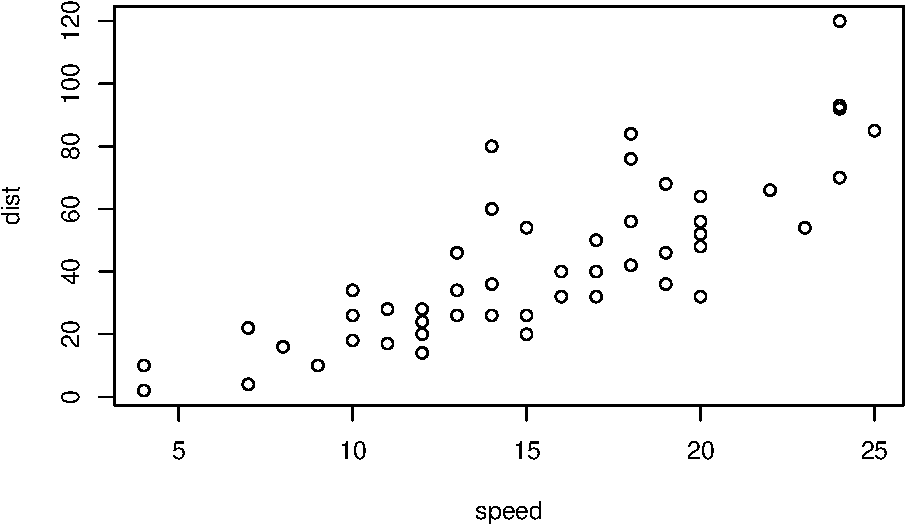
\includegraphics{24-rbasics_files/figure-latex/unnamed-chunk-4-1.pdf}

右下の、窓枠の、Plots に、上のグラフ(散布図)が表示されると思います。Export と書いてある、プルダウンメニューがあり、そこから、画像として保存することも、可能です。

以前は、このように取り出した画像を、Word などに貼り付けて、使っていました。現在でも、そのような方法を知っていることは有効だと思います。

\hypertarget{ux30a2ux30b5ux30a4ux30f3ux30e1ux30f3ux30c8ux30d8ux30ebux30d7}{%
\subsection{アサインメント、ヘルプ}\label{ux30a2ux30b5ux30a4ux30f3ux30e1ux30f3ux30c8ux30d8ux30ebux30d7}}

コンソールで次のそれぞれを、試してみてください。

\begin{itemize}
\tightlist
\item
  \texttt{df\ \textless{}-\ cars}
\end{itemize}

\texttt{df} に、\texttt{cars} をアサインします。すなわち、\texttt{df} が、\texttt{cars} の内容に置き換わります。\texttt{cars} はデータですが、データを含む、オブジェクトの名前を設定するためにも使います。オブジェクト名は。英文字から始まれば、かなりの自由度がありますが、わたしは、英文字と数字と \texttt{\_}(underscore) 程度しか使わないようにしています。

\begin{itemize}
\tightlist
\item
  \texttt{head(df)}
\end{itemize}

\texttt{head(df)} は、\texttt{head(cars)} と同じ出力が得られます。

\begin{itemize}
\tightlist
\item
  \texttt{View(cars)}
\end{itemize}

左上の、窓枠が開き、\texttt{cars} というデータ の内容が表示されます。列名のところには、三角形も表示され、それを用いると、大きい順、小さい順などに、並び替えることも可能です。また、フィルター機能も使えます。

\begin{itemize}
\tightlist
\item
  \texttt{?cars}
\end{itemize}

右下の、窓枠の Help タブに、\texttt{cars} の情報が表示されます。Help タブにある、虫眼鏡がついた、検索窓(search window)に、\texttt{cars} といれても、同じ結果が得られます。 内容を確認してください。

一番上には \texttt{cars\ \{datasets\}} とありますが、これは、\texttt{datasets} というパッケージの、\texttt{cars} だという意味です。そこで、\texttt{datasets} を調べてみましょう。

\begin{itemize}
\tightlist
\item
  \texttt{?datasets}
\end{itemize}

``The R Datasets Package'' だと書かれていて、さらに、

This package contains a variety of datasets. For a complete list, use library(help = ``datasets'').

さまざまなデータが含まれています。全てのリストをみるには、\texttt{library(help\ =\ "datasets")} を使ってください。

とありますから、\texttt{library(help\ =\ "datasets")} をコンソールに入力してみてください。

\begin{itemize}
\tightlist
\item
  \texttt{library(help\ =\ "datasets")}
\end{itemize}

左上の窓枠に、リストが表示されます。古いデータばかりですが、例として使うには、十分すぎるぐらいの、数のデータがあります。これらは、Toy Data(おもちゃのデータ)と呼ばれることもあります。

\texttt{cars} も見つかりましたか。

\hypertarget{ux304aux3059ux3059ux3081}{%
\subsection{おすすめ}\label{ux304aux3059ux3059ux3081}}

コンピュータのシステムが、日本語であると、R の言語も日本語になっているはずです。そこで、エラーが発生すると、一部、日本語で表示されます。しかし、ネット上などで、そのエラーの対応を検索するときは、英語のエラーメッセージで検索した方が、解決方法が得られる可能性が圧倒的に高いので、わたしは、英語に設定しています。英語にするには、Console で次のようにします。

言語を英語に設定:\texttt{Sys.setenv(LANG\ =\ "en")}

RStudio を終了して、もう一度起動すると、日本語に戻っていると思います。ですから、作業の最初、または、エラーが出たら、変更することをお勧めします。

日本語に戻したいときは、次のようにします。

言語を日本語に設定:\texttt{Sys.setenv(LANG\ =\ "ja")}

さまざまな Help なども、すべて日本語で表示されれば日本語を使うのは有効かもしれませんが、すくなくとも、現在は、そうではないので、上に説明したことから、英語に設定することをお勧めします。

\hypertarget{ux7df4ux7fd2-1}{%
\subsection{練習}\label{ux7df4ux7fd2-1}}

\begin{enumerate}
\def\labelenumi{\arabic{enumi}.}
\tightlist
\item
  \texttt{head(cars,\ 10L)} は何が出力されますか。\texttt{head(cars,\ n=10L)} と同じですか。
\item
  \texttt{?head} または、Help の検索窓に \texttt{head} と入力して、説明を見てみてください。\texttt{head(cars,\ n=10L)} などについて、書いてありましたか。他には、どのようなことが分かりましたか。
\item
  \texttt{datasets} のデータのいくつかについて、そのデータの help や、\texttt{head}, \texttt{str}, \texttt{summary} などを使ってみてください。これらで表示できない場合はありますか。データについては、最初に、これら、三つを試してみることをお勧めします。わかったことをメモしておくと良いでしょう。\texttt{datasets} のリストをみるには、\texttt{library(help\ =\ "datasets")} でしたね。
\end{enumerate}

\hypertarget{rstudio-ux306bux3064ux3044ux3066}{%
\section{RStudio について}\label{rstudio-ux306bux3064ux3044ux3066}}

RStudio は多くの機能を持っています。

\hypertarget{ux56dbux3064ux306eux7a93ux67a0ux3068ux30bfux30d6-four-panes-and-tabs}{%
\subsection{四つの窓枠とタブ Four Panes and Tabs}\label{ux56dbux3064ux306eux7a93ux67a0ux3068ux30bfux30d6-four-panes-and-tabs}}

\begin{itemize}
\tightlist
\item
  左上(Top Left): スクリプトや文書、データなどの編集(Source Editor)
\item
  右上(Top Right): 環境変数(Environment), 履歴(History) など(etc.)
\item
  左下(Bottom Left): コードの実行・実行結果などを表示するコンソール(Console), コンピュータシステムの端末(Terminal), 文書の機械語翻訳(Render), 背後での作業(Background Jobs)
\item
  右下(Bottom Right): ファイル(Files), 描画(Plots), パッケージ(Packages), ヘルプ(Help), 文書などの表示窓(Viewer), R Markdown の HTML, PDF 表示(Presentation\footnote{Viewerへの表示を使っており、Presentationへの表示を使っておらず不明})
\end{itemize}

\hypertarget{r-script-ux5b9fux884cux8a18ux9332}{%
\section{R Script 実行記録}\label{r-script-ux5b9fux884cux8a18ux9332}}

R Script を使って、コードを実行すると、その記録を残すことができます。

\hypertarget{r-script-ux306eux4f5cux6210}{%
\subsection{R Script の作成}\label{r-script-ux306eux4f5cux6210}}

\begin{itemize}
\tightlist
\item
  RStudio の上のメニュー・バーからFile \textgreater{} New File \textgreater{} R Script を選択します。
\item
  File \textgreater{} Save As で、名前をつけて保存します。\{file\_name\}.R が作成されます。

  \begin{itemize}
  \tightlist
  \item
    右下の、Files から、ファイルを確認してください。
  \end{itemize}
\item
  \texttt{head(cars)}, \texttt{str(cars)}, \texttt{summary(cars)}, \texttt{plot(cars)} などと改行をしながらコードを書きます。
\item
  実行するには、カーソルの場所で Ctrl+Shift+Enter (Win) または Cmd+Shift+Enter (Mac) とすると、カーソルのある行か、その下の行で、最初のコードが実行されます。

  \begin{itemize}
  \tightlist
  \item
    R Script エディターの上にある、Run ボタンを押しても、同様に実行されます。
  \item
    Run ボタンの右の、Source ボタンを押すと、そのスクリプトの、最初からすべてが実行されます。
  \end{itemize}
\item
  最後には保存しておきましょう。たとえば、\texttt{myfirstscript} などとすると、File のところに、\texttt{myfirstscript.R} というファイルができていることを確認できます。
\end{itemize}

\hypertarget{r-script-ux306bux3088ux308bux5b9fux884c}{%
\subsection{R Script による実行}\label{r-script-ux306bux3088ux308bux5b9fux884c}}

新しく、R Script を作成し、この下の、コード(ハイライトされている部分)をコピー・ペーストして、保存し、実行してみてください。

それぞれ、どのようなことをしているでしょうか。

\hypertarget{ux30b9ux30afux30eaux30d7ux30c81-basics.r}{%
\subsubsection{\texorpdfstring{スクリプト1: \texttt{basics.R}}{スクリプト1: basics.R}}\label{ux30b9ux30afux30eaux30d7ux30c81-basics.r}}

\begin{Shaded}
\begin{Highlighting}[]
\DocumentationTok{\#\#\#\#\#\#\#\#\#\#\#\#\#\#\#\#\#}
\CommentTok{\#}
\CommentTok{\# basics.R}
\CommentTok{\#}
\DocumentationTok{\#\#\#\#\#\#\#\#\#\#\#\#\#\#\#\#}
\CommentTok{\# \textquotesingle{}Quick R\textquotesingle{} by DataCamp may be a handy reference: }
\CommentTok{\#     https://www.statmethods.net/management/index.html}
\CommentTok{\# Cheat Sheet at RStudio: https://www.rstudio.com/resources/cheatsheets/}
\CommentTok{\# Base R Cheat Sheet: https://github.com/rstudio/cheatsheets/raw/main/base{-}r.pdf}
\CommentTok{\# To execute the line: Control + Enter (Window and Linux), Command + Enter (Mac)}
\DocumentationTok{\#\# try your experiments on the console}

\DocumentationTok{\#\# calculator}

\DecValTok{3} \SpecialCharTok{+} \DecValTok{7}

\DocumentationTok{\#\#\# +, {-}, *, /, \^{} (or **), \%\%, \%/\%}

\DecValTok{3} \SpecialCharTok{+} \DecValTok{10} \SpecialCharTok{/} \DecValTok{2}

\DecValTok{3}\SpecialCharTok{\^{}}\DecValTok{2}

\DecValTok{2}\SpecialCharTok{\^{}}\DecValTok{3}

\DecValTok{2}\SpecialCharTok{*}\DecValTok{2}\SpecialCharTok{*}\DecValTok{2}

\DocumentationTok{\#\#\# assignment: \textless{}{-}, (=, {-}\textgreater{}, assign()) }

\NormalTok{x }\OtherTok{\textless{}{-}} \DecValTok{5}

\NormalTok{x }

\DocumentationTok{\#\#\#\# object\_name \textless{}{-} value, \textquotesingle{}\textless{}{-}\textquotesingle{} shortcut: Alt (option) + \textquotesingle{}{-}\textquotesingle{} (hyphen or minus) }
\DocumentationTok{\#\#\#\# Object names must start with a letter and can only contain letter, numbers, \_ and .}

\NormalTok{this\_is\_a\_long\_name }\OtherTok{\textless{}{-}} \DecValTok{5}\SpecialCharTok{\^{}}\DecValTok{3}

\NormalTok{this\_is\_a\_long\_name}

\NormalTok{char\_name }\OtherTok{\textless{}{-}} \StringTok{"What is your name?"}

\NormalTok{char\_name}

\DocumentationTok{\#\#\#\# Use \textquotesingle{}tab completion\textquotesingle{} and \textquotesingle{}up arrow\textquotesingle{}}

\DocumentationTok{\#\#\# ls(): list of all assignments}

\FunctionTok{ls}\NormalTok{()}
\FunctionTok{ls.str}\NormalTok{()}

\DocumentationTok{\#\#\#\# check Environment in the upper right pane}

\DocumentationTok{\#\#\# (atomic) vectors}

\DecValTok{5}\SpecialCharTok{:}\DecValTok{10}

\NormalTok{a }\OtherTok{\textless{}{-}} \FunctionTok{seq}\NormalTok{(}\DecValTok{5}\NormalTok{,}\DecValTok{10}\NormalTok{)}

\NormalTok{a}

\NormalTok{b }\OtherTok{\textless{}{-}} \DecValTok{5}\SpecialCharTok{:}\DecValTok{10}

\FunctionTok{identical}\NormalTok{(a,b)}

\FunctionTok{seq}\NormalTok{(}\DecValTok{5}\NormalTok{,}\DecValTok{10}\NormalTok{,}\DecValTok{2}\NormalTok{) }\CommentTok{\# same as seq(from = 5, to = 10, by = 2)}

\NormalTok{c1 }\OtherTok{\textless{}{-}} \FunctionTok{seq}\NormalTok{(}\DecValTok{0}\NormalTok{,}\DecValTok{100}\NormalTok{, }\AttributeTok{by =} \DecValTok{10}\NormalTok{)}

\NormalTok{c2 }\OtherTok{\textless{}{-}} \FunctionTok{seq}\NormalTok{(}\DecValTok{0}\NormalTok{,}\DecValTok{100}\NormalTok{, }\AttributeTok{length.out =} \DecValTok{10}\NormalTok{)}

\NormalTok{c1}

\NormalTok{c2}

\FunctionTok{length}\NormalTok{(c1)}

\DocumentationTok{\#\#\#\# ? seq   ? length   ? identical}

\NormalTok{(die }\OtherTok{\textless{}{-}} \DecValTok{1}\SpecialCharTok{:}\DecValTok{6}\NormalTok{)}

\NormalTok{zero\_one }\OtherTok{\textless{}{-}} \FunctionTok{c}\NormalTok{(}\DecValTok{0}\NormalTok{,}\DecValTok{1}\NormalTok{) }\CommentTok{\# same as 0:1}

\NormalTok{die }\SpecialCharTok{+}\NormalTok{ zero\_one }\CommentTok{\# c(1,2,3,4,5,6) + c(0,1). re{-}use}

\NormalTok{d1 }\OtherTok{\textless{}{-}} \FunctionTok{rep}\NormalTok{(}\DecValTok{1}\SpecialCharTok{:}\DecValTok{3}\NormalTok{,}\DecValTok{2}\NormalTok{) }\CommentTok{\# repeat}


\NormalTok{d1}

\NormalTok{die }\SpecialCharTok{==}\NormalTok{ d1}

\NormalTok{d2 }\OtherTok{\textless{}{-}} \FunctionTok{as.character}\NormalTok{(die }\SpecialCharTok{==}\NormalTok{ d1)}

\NormalTok{d2}

\NormalTok{d3 }\OtherTok{\textless{}{-}} \FunctionTok{as.numeric}\NormalTok{(die }\SpecialCharTok{==}\NormalTok{ d1)}

\NormalTok{d3}

\DocumentationTok{\#\#\# class() for class and typeof() for mode}
\DocumentationTok{\#\#\# class of vectors: numeric, charcters, logical}
\DocumentationTok{\#\#\# types of vectors: doubles, integers, characters, logicals (complex and raw)}

\FunctionTok{typeof}\NormalTok{(d1); }\FunctionTok{class}\NormalTok{(d1)}

\FunctionTok{typeof}\NormalTok{(d2); }\FunctionTok{class}\NormalTok{(d2)}

\FunctionTok{typeof}\NormalTok{(d3); }\FunctionTok{class}\NormalTok{(d3)}

\FunctionTok{sqrt}\NormalTok{(}\DecValTok{2}\NormalTok{)}

\FunctionTok{sqrt}\NormalTok{(}\DecValTok{2}\NormalTok{)}\SpecialCharTok{\^{}}\DecValTok{2}

\FunctionTok{sqrt}\NormalTok{(}\DecValTok{2}\NormalTok{)}\SpecialCharTok{\^{}}\DecValTok{2} \SpecialCharTok{{-}} \DecValTok{2}

\FunctionTok{typeof}\NormalTok{(}\FunctionTok{sqrt}\NormalTok{(}\DecValTok{2}\NormalTok{))}

\FunctionTok{typeof}\NormalTok{(}\DecValTok{2}\NormalTok{)}

\FunctionTok{typeof}\NormalTok{(2L)}

\DecValTok{5} \SpecialCharTok{==} \FunctionTok{c}\NormalTok{(}\DecValTok{5}\NormalTok{)}

\FunctionTok{length}\NormalTok{(}\DecValTok{5}\NormalTok{)}

\DocumentationTok{\#\#\# Subsetting}

\NormalTok{(A\_Z }\OtherTok{\textless{}{-}}\NormalTok{ LETTERS)}

\NormalTok{A\_F }\OtherTok{\textless{}{-}}\NormalTok{ A\_Z[}\DecValTok{1}\SpecialCharTok{:}\DecValTok{6}\NormalTok{]}

\NormalTok{A\_F}

\NormalTok{A\_F[}\DecValTok{3}\NormalTok{]}

\NormalTok{A\_F[}\FunctionTok{c}\NormalTok{(}\DecValTok{3}\NormalTok{,}\DecValTok{5}\NormalTok{)]}

\NormalTok{large }\OtherTok{\textless{}{-}}\NormalTok{ die }\SpecialCharTok{\textgreater{}} \DecValTok{3}

\NormalTok{large}

\NormalTok{even }\OtherTok{\textless{}{-}}\NormalTok{ die }\SpecialCharTok{\%in\%} \FunctionTok{c}\NormalTok{(}\DecValTok{2}\NormalTok{,}\DecValTok{4}\NormalTok{,}\DecValTok{6}\NormalTok{)}

\NormalTok{even}

\NormalTok{A\_F[large]}

\NormalTok{A\_F[even]}

\NormalTok{A\_F[die }\SpecialCharTok{\textless{}} \DecValTok{4}\NormalTok{]}

\DocumentationTok{\#\#\# Compare df with df1 \textless{}{-} data.frame(number = die, alphabet = A\_F)}
\NormalTok{df }\OtherTok{\textless{}{-}} \FunctionTok{data.frame}\NormalTok{(}\AttributeTok{number =}\NormalTok{ die, }\AttributeTok{alphabet =}\NormalTok{ A\_F, }\AttributeTok{stringsAsFactors =} \ConstantTok{FALSE}\NormalTok{)}

\NormalTok{df}

\NormalTok{df}\SpecialCharTok{$}\NormalTok{number}

\NormalTok{df}\SpecialCharTok{$}\NormalTok{alphabet}

\NormalTok{df[}\DecValTok{3}\NormalTok{,}\DecValTok{2}\NormalTok{]}

\NormalTok{df[}\DecValTok{4}\NormalTok{,}\DecValTok{1}\NormalTok{]}

\NormalTok{df[}\DecValTok{1}\NormalTok{]}

\FunctionTok{class}\NormalTok{(df[}\DecValTok{1}\NormalTok{])}

\FunctionTok{class}\NormalTok{(df[[}\DecValTok{1}\NormalTok{]])}

\FunctionTok{identical}\NormalTok{(df[[}\DecValTok{1}\NormalTok{]], die)}

\FunctionTok{identical}\NormalTok{(df[}\DecValTok{1}\NormalTok{],die)}

\DocumentationTok{\#\#\#\#\#\#\#\#\#\#\#\#\#\#\#\#\#\#\#\#}
\CommentTok{\# The First Example}
\DocumentationTok{\#\#\#\#\#\#\#\#\#\#\#\#\#\#\#\#\#\#\#\#}

\FunctionTok{plot}\NormalTok{(cars)}

\CommentTok{\# Help}

\NormalTok{? cars}

\CommentTok{\# cars is in the \textquotesingle{}datasets\textquotesingle{} package}

\FunctionTok{data}\NormalTok{()}

\CommentTok{\# help(cars) does the same as ? cars}
\CommentTok{\# You can use Help tab in the right bottom pane}

\FunctionTok{help}\NormalTok{(plot)}
\NormalTok{? par}

\FunctionTok{head}\NormalTok{(cars)}

\FunctionTok{str}\NormalTok{(cars)}

\FunctionTok{summary}\NormalTok{(cars)}

\NormalTok{x }\OtherTok{\textless{}{-}}\NormalTok{ cars}\SpecialCharTok{$}\NormalTok{speed}
\NormalTok{y }\OtherTok{\textless{}{-}}\NormalTok{ cars}\SpecialCharTok{$}\NormalTok{dist}

\FunctionTok{min}\NormalTok{(x)}
\FunctionTok{mean}\NormalTok{(x)}
\FunctionTok{quantile}\NormalTok{(x)}

\FunctionTok{plot}\NormalTok{(cars)}

\FunctionTok{abline}\NormalTok{(}\FunctionTok{lm}\NormalTok{(cars}\SpecialCharTok{$}\NormalTok{dist }\SpecialCharTok{\textasciitilde{}}\NormalTok{ cars}\SpecialCharTok{$}\NormalTok{speed))}

\FunctionTok{summary}\NormalTok{(}\FunctionTok{lm}\NormalTok{(cars}\SpecialCharTok{$}\NormalTok{dist }\SpecialCharTok{\textasciitilde{}}\NormalTok{ cars}\SpecialCharTok{$}\NormalTok{speed))}

\FunctionTok{boxplot}\NormalTok{(cars)}

\FunctionTok{hist}\NormalTok{(cars}\SpecialCharTok{$}\NormalTok{speed)}
\FunctionTok{hist}\NormalTok{(cars}\SpecialCharTok{$}\NormalTok{dist)}
\FunctionTok{hist}\NormalTok{(cars}\SpecialCharTok{$}\NormalTok{dist, }\AttributeTok{breaks =} \FunctionTok{seq}\NormalTok{(}\DecValTok{0}\NormalTok{,}\DecValTok{120}\NormalTok{, }\DecValTok{10}\NormalTok{))}
\end{Highlighting}
\end{Shaded}

\hypertarget{ux30b9ux30afux30eaux30d7ux30c82-coronavirus.r}{%
\subsubsection{\texorpdfstring{スクリプト2: \texttt{coronavirus.R}}{スクリプト2: coronavirus.R}}\label{ux30b9ux30afux30eaux30d7ux30c82-coronavirus.r}}

\begin{Shaded}
\begin{Highlighting}[]
\CommentTok{\# https://coronavirus.jhu.edu/map.html}
\CommentTok{\# JHU Covid{-}19 global time series data}
\CommentTok{\# See R package coronavirus at: https://github.com/RamiKrispin/coronavirus}
\CommentTok{\# Data taken from: https://github.com/RamiKrispin/coronavirus/tree/master/csv}
\CommentTok{\# Last Updated}
\FunctionTok{Sys.Date}\NormalTok{()}

\DocumentationTok{\#\# Download and read csv (comma separated value) file}
\NormalTok{coronavirus }\OtherTok{\textless{}{-}} \FunctionTok{read.csv}\NormalTok{(}\StringTok{"https://github.com/RamiKrispin/coronavirus/raw/master/csv/coronavirus.csv"}\NormalTok{)}
\CommentTok{\# write.csv(coronavirus, "data/coronavirus.csv")}

\DocumentationTok{\#\# Summaries and structures of the data}
\FunctionTok{head}\NormalTok{(coronavirus)}
\FunctionTok{str}\NormalTok{(coronavirus)}
\NormalTok{coronavirus}\SpecialCharTok{$}\NormalTok{date }\OtherTok{\textless{}{-}} \FunctionTok{as.Date}\NormalTok{(coronavirus}\SpecialCharTok{$}\NormalTok{date)}
\FunctionTok{str}\NormalTok{(coronavirus)}

\FunctionTok{range}\NormalTok{(coronavirus}\SpecialCharTok{$}\NormalTok{date)}
\FunctionTok{unique}\NormalTok{(coronavirus}\SpecialCharTok{$}\NormalTok{country)}
\FunctionTok{unique}\NormalTok{(coronavirus}\SpecialCharTok{$}\NormalTok{type)}

\DocumentationTok{\#\# Set Country}
\NormalTok{COUNTRY }\OtherTok{\textless{}{-}} \StringTok{"Japan"}
\NormalTok{df0 }\OtherTok{\textless{}{-}}\NormalTok{ coronavirus[coronavirus}\SpecialCharTok{$}\NormalTok{country }\SpecialCharTok{==}\NormalTok{ COUNTRY,]}
\FunctionTok{head}\NormalTok{(df0)}
\FunctionTok{tail}\NormalTok{(df0)}
\NormalTok{(pop }\OtherTok{\textless{}{-}}\NormalTok{ df0}\SpecialCharTok{$}\NormalTok{population[}\DecValTok{1}\NormalTok{])}
\NormalTok{df }\OtherTok{\textless{}{-}}\NormalTok{ df0[}\FunctionTok{c}\NormalTok{(}\DecValTok{1}\NormalTok{,}\DecValTok{6}\NormalTok{,}\DecValTok{7}\NormalTok{,}\DecValTok{13}\NormalTok{)]}
\FunctionTok{str}\NormalTok{(df)}
\FunctionTok{head}\NormalTok{(df)}
\DocumentationTok{\#\#\# alternatively,}
\FunctionTok{head}\NormalTok{(df0[}\FunctionTok{c}\NormalTok{(}\StringTok{"date"}\NormalTok{, }\StringTok{"type"}\NormalTok{, }\StringTok{"cases"}\NormalTok{, }\StringTok{"population"}\NormalTok{)])}
\DocumentationTok{\#\#\#}

\DocumentationTok{\#\# Set types}
\NormalTok{df\_confirmed }\OtherTok{\textless{}{-}}\NormalTok{ df[df}\SpecialCharTok{$}\NormalTok{type }\SpecialCharTok{==} \StringTok{"confirmed"}\NormalTok{,]}
\NormalTok{df\_death }\OtherTok{\textless{}{-}}\NormalTok{ df[df}\SpecialCharTok{$}\NormalTok{type }\SpecialCharTok{==} \StringTok{"death"}\NormalTok{,]}
\NormalTok{df\_recovery }\OtherTok{\textless{}{-}}\NormalTok{ df[df}\SpecialCharTok{$}\NormalTok{data\_type }\SpecialCharTok{==} \StringTok{"recovery"}\NormalTok{,]}
\FunctionTok{head}\NormalTok{(df\_confirmed)}
\FunctionTok{head}\NormalTok{(df\_death)}
\FunctionTok{head}\NormalTok{(df\_recovery)}

\DocumentationTok{\#\# Histogram}
\FunctionTok{plot}\NormalTok{(df\_confirmed}\SpecialCharTok{$}\NormalTok{date, df\_confirmed}\SpecialCharTok{$}\NormalTok{cases, }\AttributeTok{type =} \StringTok{"h"}\NormalTok{)}
\FunctionTok{plot}\NormalTok{(df\_death}\SpecialCharTok{$}\NormalTok{date, df\_death}\SpecialCharTok{$}\NormalTok{cases, }\AttributeTok{type =} \StringTok{"h"}\NormalTok{)}
\CommentTok{\# plot(df\_recovered$date, df\_recovered$cases, type = "h") \# no data for recovery}

\DocumentationTok{\#\# Scatter plot and correlation}
\FunctionTok{plot}\NormalTok{(df\_confirmed}\SpecialCharTok{$}\NormalTok{cases, df\_death}\SpecialCharTok{$}\NormalTok{cases, }\AttributeTok{type =} \StringTok{"p"}\NormalTok{)}
\FunctionTok{cor}\NormalTok{(df\_confirmed}\SpecialCharTok{$}\NormalTok{cases, df\_death}\SpecialCharTok{$}\NormalTok{cases)}


\DocumentationTok{\#\# In addition set a period}
\NormalTok{start\_date }\OtherTok{\textless{}{-}} \FunctionTok{as.Date}\NormalTok{(}\StringTok{"2022{-}07{-}01"}\NormalTok{)}
\NormalTok{end\_date }\OtherTok{\textless{}{-}} \FunctionTok{Sys.Date}\NormalTok{() }
\NormalTok{df\_date }\OtherTok{\textless{}{-}}\NormalTok{ df[df}\SpecialCharTok{$}\NormalTok{date }\SpecialCharTok{\textgreater{}=}\NormalTok{start\_date }\SpecialCharTok{\&}\NormalTok{ df}\SpecialCharTok{$}\NormalTok{date }\SpecialCharTok{\textless{}=}\NormalTok{ end\_date,]}
\DocumentationTok{\#\#}

\DocumentationTok{\#\# Set types}
\NormalTok{df\_date\_confirmed }\OtherTok{\textless{}{-}}\NormalTok{ df\_date[df\_date}\SpecialCharTok{$}\NormalTok{type }\SpecialCharTok{==} \StringTok{"confirmed"}\NormalTok{,]}
\NormalTok{df\_date\_death }\OtherTok{\textless{}{-}}\NormalTok{ df\_date[df\_date}\SpecialCharTok{$}\NormalTok{type }\SpecialCharTok{==} \StringTok{"death"}\NormalTok{,]}
\NormalTok{df\_date\_recovery }\OtherTok{\textless{}{-}}\NormalTok{ df\_date[df\_date}\SpecialCharTok{$}\NormalTok{data\_type }\SpecialCharTok{==} \StringTok{"recovery"}\NormalTok{,]}
\FunctionTok{head}\NormalTok{(df\_date\_confirmed)}
\FunctionTok{head}\NormalTok{(df\_date\_death)}
\FunctionTok{head}\NormalTok{(df\_date\_recovery)}

\DocumentationTok{\#\# Histogram}
\FunctionTok{plot}\NormalTok{(df\_date\_confirmed}\SpecialCharTok{$}\NormalTok{date, df\_date\_confirmed}\SpecialCharTok{$}\NormalTok{cases, }\AttributeTok{type =} \StringTok{"h"}\NormalTok{)}
\FunctionTok{plot}\NormalTok{(df\_date\_death}\SpecialCharTok{$}\NormalTok{date, df\_date\_death}\SpecialCharTok{$}\NormalTok{cases, }\AttributeTok{type =} \StringTok{"h"}\NormalTok{)}
\CommentTok{\# plot(df\_date\_recovered$date, df\_date\_recovered$cases, type = "h") \# no data for recovery}

\FunctionTok{plot}\NormalTok{(df\_date\_confirmed}\SpecialCharTok{$}\NormalTok{cases, df\_date\_death}\SpecialCharTok{$}\NormalTok{cases, }\AttributeTok{type =} \StringTok{"p"}\NormalTok{)}
\FunctionTok{cor}\NormalTok{(df\_date\_confirmed}\SpecialCharTok{$}\NormalTok{cases, df\_date\_death}\SpecialCharTok{$}\NormalTok{cases)}

\DocumentationTok{\#\#\#\# Extra}
\FunctionTok{plot}\NormalTok{(df\_confirmed}\SpecialCharTok{$}\NormalTok{date, df\_confirmed}\SpecialCharTok{$}\NormalTok{cases, }\AttributeTok{type =} \StringTok{"h"}\NormalTok{, }
     \AttributeTok{main =} \FunctionTok{paste}\NormalTok{(}\StringTok{"Comfirmed Cases in"}\NormalTok{,COUNTRY), }
     \AttributeTok{xlab =} \StringTok{"Date"}\NormalTok{, }\AttributeTok{ylab =} \StringTok{"Number of Cases"}\NormalTok{)}
\end{Highlighting}
\end{Shaded}

\hypertarget{ux7df4ux7fd2-2}{%
\subsection{練習}\label{ux7df4ux7fd2-2}}

上の、\texttt{coronavirus.R} について

\begin{enumerate}
\def\labelenumi{\arabic{enumi}.}
\tightlist
\item
  \texttt{COUNTRY\ \textless{}-\ "Japan"} の Japan を他の国に変えてみましょう。
\item
  \texttt{start\_date\ \textless{}-\ as.Date("2022-07-01")} の日付を、他の日付に変えてみましょう。
\item
  \texttt{df\_confirmed\$cases} と \texttt{df\_death\$cases} についてどんなことがわかりますか。
\item
  発見や、問いがあれば、書き出してみましょう。
\end{enumerate}

\hypertarget{tips}{%
\subsection{Tips}\label{tips}}

キーボード・ショートカットと言われる、さまざまな機能があります。

\begin{itemize}
\tightlist
\item
  上のメニュー・バー: Help \textgreater{} Keyboard Short Cut Help 確認してみてください。
\item
  右下の窓枠: Files タブから、ファイルの確認ができます。
\end{itemize}

\hypertarget{ux30d1ux30c3ux30b1ux30fcux30b8---packages}{%
\section{パッケージ - Packages}\label{ux30d1ux30c3ux30b1ux30fcux30b8---packages}}

\begin{quote}
R packages are extensions to the R statistical programming language containing code, data, and documentation in a standardised collection format that can be installed by users of R using Tool \textgreater{} Install Packages in the top menu bar of R Studio. \url{https://en.wikipedia.org/wiki/R_package}
\end{quote}

\begin{quote}
Rパッケージは、Rの拡張機能で、コード、データ、ドキュメントを標準化されたコレクション形式で含んでおり、標準的なものは、R Studio の Top Bar の Tool \textgreater{} Install Packages からインストールできます。
\end{quote}

\hypertarget{ux30d1ux30c3ux30b1ux30fcux30b8ux306eux30a4ux30f3ux30b9ux30c8ux30fcux30eb}{%
\subsection{パッケージのインストール}\label{ux30d1ux30c3ux30b1ux30fcux30b8ux306eux30a4ux30f3ux30b9ux30c8ux30fcux30eb}}

いずれ使いますので、まずは、三つのパッケージをインストールしてみましょう。

\begin{itemize}
\tightlist
\item
  \texttt{tidyverse}
\item
  \texttt{rmarkdown}
\item
  \texttt{tinytex}
\end{itemize}

インストール方法はいくつかあります。

一つ目は、上のメニューバーの Tool から、Install Packages \ldots{} を選択します。そして、パッケージーズにインストールしたい、パッケージ名を入力します。そのパッケージ名が下にも出れば、Install ボタンを押してください。入力した名前の下にパッケージ名が出ない場合は、スペルが間違っている可能性がありますから、確認して、入れ直してください。

Console に、\texttt{install.packages("tidyverse")} などと表示され、たくさんメッセージが出ます。終了すると、\textgreater{} のマークがでます。

二つ目は、\texttt{install.packages("tidyverse")} のような書式で書いて、Console に入れる方法です。

三つ目は、右下の窓枠の Packages のタブにある、Install というボタンを押す方法です。すると、一番目の方法に、戻り、パッケージ名を入力できるようになります。

この Packages タブにある、ものが、すでに、インストールされているパッケージです。そのなかで、\texttt{base} や、\texttt{datasets} などいくつかに、チェックがついていると思いますが、それらは、ロードされていて、いつでも、使える状態になっていることを意味しています。ロードは、たとえば、\texttt{library(tidyverse)} のようにしますが、それは、いずれもう一度説明します。

インストールは一回だけ。ときどき、Tools \textgreater{} Check for Package Update をつかって、Update しておくと良いでしょう。

パッケージのインストールで問題が生じることがあります。特に、Windows の日本語システムの場合です。(4.3.2 R Studio の インストール の下に書いてある部分を参照してください。)

回避方法もいくつかあるようですが、混乱をさけるため、その場合は、Posit Cloud(旧:RStudio Cloud)を使うと良いでしょう。それを見越して、最初は、Posit Cloud ではじめることを、わたしはお薦めしています。自分のコンピュータで、R が RStudio 上で問題なく動いていても、Cloud 上にアカウントを持っていて、実行できることは有効ですし、全員が、同じ環境で作業できることもたいせつなことです。他にも、すぐ、Cheat Sheets(早見表)や、Posit Primers という練習問題(Tutorial)を利用できたり、プロジェクトを共有したりなど、さまざまなメリットがあります。

\hypertarget{ux5099ux8003}{%
\subsection{備考}\label{ux5099ux8003}}

Package によっては、Source から Compile するかと聞いてくる場合があります。どちらでも、良いのですが、特に、問題が起こっていなければ、No でよいと思います。コンピュータにあった形でインストールすることが必要な場合は、Yes とします。

同じパッケージをもう一度、インストールしたり、または、関連するパッケージがあるような場合、R をリスタートするかと聞いてくることがあります。特に問題が起こらなければ、No で構いません。ただ、エラーが起こって、それに関連して、特別なパッケージをインストールする必要がある場合がありますが、そのときは、Yes としてください。

\hypertarget{ux7df4ux7fd2ux554fux984c-posit-primers}{%
\section{練習問題 Posit Primers}\label{ux7df4ux7fd2ux554fux984c-posit-primers}}

Posit Primers \url{https://posit.cloud/learn/primers}

教科書 \href{https://r4ds.had.co.nz}{``R for Data Science''} は、\texttt{tidyverse} パッケージを中心に、データサイエンスについて解説したものですが、Posit Primers は、演習問題をしながら、教科書の内容を理解できるように構成されています。

Posit Cloud からは、左のメニュー(隠れている場合は左上の3本線をクリックして表示させて)から選ぶことができます。そうでない場合は、直接、上のリンクから、利用してください。

\hypertarget{ux6700ux521dux306eux6f14ux7fd2-the-basics-r4ds-explore-i}{%
\subsection{最初の演習 The Basics -- r4ds: Explore, I}\label{ux6700ux521dux306eux6f14ux7fd2-the-basics-r4ds-explore-i}}

\begin{itemize}
\tightlist
\item
  \href{https://rstudio.cloud/learn/primers/1.1}{Visualization Basics}
\item
  \href{https://rstudio.cloud/learn/primers/1.2}{Programming Basics}
\end{itemize}

ぜひこれら二つの演習問題を、トライしてください。解説を読んでいただけでは、データサイエンスは身につきません。

\hypertarget{ux53c2ux8003ux6587ux732e-references}{%
\section{参考文献 References}\label{ux53c2ux8003ux6587ux732e-references}}

一番目は、すでに紹介した、教科書です。二番目は、この文書を作成している、Bookdown というパッケージのサイトですが、そこに、たくさんの本が、無償で公開されています。素晴らしい本がたくさん含まれています。

\begin{itemize}
\tightlist
\item
  R For Data Science, by H. Wickham: \url{https://r4ds.had.co.nz}

  \begin{itemize}
  \tightlist
  \item
    Introduction: \url{https://r4ds.had.co.nz/explore-intro.html\#explore-intro}
  \end{itemize}
\item
  Bookdown: \url{https://bookdown.org}, \href{https://bookdown.org/home/archive/}{Archive}
\end{itemize}

下の一番目は、R 入門を、2時限の講義でしたときのものです。二番目と三番目は、講義で使ったものを、まとめたものです。教科書のようには、できていませんが、参考になる部分もあるかと思いますので、紹介しておきます。

\begin{itemize}
\tightlist
\item
  \href{https://ds-sl.github.io/intro2r/intro2r.nb.html}{Introducton to R}
\item
  \href{https://icu-hsuzuki.github.io/da4r2022/}{Data Analysis for Researchers 2022}
\item
  \href{https://icu-hsuzuki.github.io/da4r2021/}{Data Analysis for Researchers 2021}
\end{itemize}

\hypertarget{youtube-video---getstarted}{%
\section{YouTube Video - getstarted}\label{youtube-video---getstarted}}

\begin{itemize}
\tightlist
\item
  ファイル:\url{https://ds-sl.github.io/intro2r/getstarted.html}
\end{itemize}

\hypertarget{part-part-iii-institutional-data}{%
\part{PART III INSTITUTIONAL DATA}\label{part-part-iii-institutional-data}}

\hypertarget{worldbank}{%
\chapter{World Bank}\label{worldbank}}

\hypertarget{world-development-indicator-wdi}{%
\section{World Development Indicator (WDI)}\label{world-development-indicator-wdi}}

パッケージ と \texttt{tidyverse} と \texttt{WDI} を使いますから、下のコードによって、ロードします。

\begin{Shaded}
\begin{Highlighting}[]
\FunctionTok{library}\NormalTok{(tidyverse)}
\CommentTok{\#\textgreater{} {-}{-} Attaching core tidyverse packages {-}{-}{-}{-} tidyverse 2.0.0 {-}{-}}
\CommentTok{\#\textgreater{} v dplyr     1.1.2     v readr     2.1.4}
\CommentTok{\#\textgreater{} v forcats   1.0.0     v stringr   1.5.0}
\CommentTok{\#\textgreater{} v ggplot2   3.4.2     v tibble    3.2.1}
\CommentTok{\#\textgreater{} v lubridate 1.9.2     v tidyr     1.3.0}
\CommentTok{\#\textgreater{} v purrr     1.0.1     }
\CommentTok{\#\textgreater{} {-}{-} Conflicts {-}{-}{-}{-}{-}{-}{-}{-}{-}{-}{-}{-}{-}{-}{-}{-}{-}{-}{-}{-}{-}{-} tidyverse\_conflicts() {-}{-}}
\CommentTok{\#\textgreater{} x dplyr::filter() masks stats::filter()}
\CommentTok{\#\textgreater{} x dplyr::lag()    masks stats::lag()}
\CommentTok{\#\textgreater{} i Use the conflicted package (\textless{}http://conflicted.r{-}lib.org/\textgreater{}) to force all conflicts to become errors}
\FunctionTok{library}\NormalTok{(WDI)}
\end{Highlighting}
\end{Shaded}

まず、三つの例を見てみましょう。なにをしているかわかりますか。考えて見てください。

\begin{Shaded}
\begin{Highlighting}[]
\FunctionTok{WDI}\NormalTok{(}\AttributeTok{country =} \StringTok{"all"}\NormalTok{, }\AttributeTok{indicator =} \FunctionTok{c}\NormalTok{(}\AttributeTok{gdp =} \StringTok{"NY.GDP.MKTP.CD"}\NormalTok{),}
    \AttributeTok{extra=}\ConstantTok{TRUE}\NormalTok{) }\SpecialCharTok{\%\textgreater{}\%} \FunctionTok{drop\_na}\NormalTok{(gdp) }\SpecialCharTok{\%\textgreater{}\%}
  \FunctionTok{filter}\NormalTok{(year}\SpecialCharTok{==}\FunctionTok{max}\NormalTok{(year), income }\SpecialCharTok{!=}\StringTok{"Aggregates"}\NormalTok{) }\SpecialCharTok{\%\textgreater{}\%} 
  \FunctionTok{drop\_na}\NormalTok{(region) }\SpecialCharTok{\%\textgreater{}\%} \FunctionTok{arrange}\NormalTok{(}\FunctionTok{desc}\NormalTok{(gdp))}
\end{Highlighting}
\end{Shaded}

\begin{verbatim}
#> Rows: 16492 Columns: 13
#> -- Column specification ------------------------------------
#> Delimiter: ","
#> chr  (7): country, iso2c, iso3c, region, capital, income...
#> dbl  (4): year, gdp, longitude, latitude
#> lgl  (1): status
#> date (1): lastupdated
#> 
#> i Use `spec()` to retrieve the full column specification for this data.
#> i Specify the column types or set `show_col_types = FALSE` to quiet this message.
#> # A tibble: 196 x 13
#>    country      iso2c iso3c  year     gdp status lastupdated
#>    <chr>        <chr> <chr> <dbl>   <dbl> <lgl>  <date>     
#>  1 United Stat~ US    USA    2021 2.33e13 NA     2022-12-22 
#>  2 China        CN    CHN    2021 1.77e13 NA     2022-12-22 
#>  3 Japan        JP    JPN    2021 4.94e12 NA     2022-12-22 
#>  4 Germany      DE    DEU    2021 4.26e12 NA     2022-12-22 
#>  5 India        IN    IND    2021 3.18e12 NA     2022-12-22 
#>  6 United King~ GB    GBR    2021 3.13e12 NA     2022-12-22 
#>  7 France       FR    FRA    2021 2.96e12 NA     2022-12-22 
#>  8 Italy        IT    ITA    2021 2.11e12 NA     2022-12-22 
#>  9 Canada       CA    CAN    2021 1.99e12 NA     2022-12-22 
#> 10 Korea, Rep.  KR    KOR    2021 1.81e12 NA     2022-12-22 
#> # i 186 more rows
#> # i 6 more variables: region <chr>, capital <chr>,
#> #   longitude <dbl>, latitude <dbl>, income <chr>,
#> #   lending <chr>
\end{verbatim}

\begin{Shaded}
\begin{Highlighting}[]
\FunctionTok{WDI}\NormalTok{(}\AttributeTok{country =} \FunctionTok{c}\NormalTok{(}\StringTok{"CN"}\NormalTok{,}\StringTok{"GB"}\NormalTok{,}\StringTok{"JP"}\NormalTok{,}\StringTok{"IN"}\NormalTok{,}\StringTok{"US"}\NormalTok{,}\StringTok{"DE"}\NormalTok{), }\AttributeTok{indicator =} \FunctionTok{c}\NormalTok{(}\AttributeTok{gdp =} \StringTok{"NY.GDP.MKTP.CD"}\NormalTok{), }\AttributeTok{extra=}\ConstantTok{TRUE}\NormalTok{) }\SpecialCharTok{\%\textgreater{}\%} \FunctionTok{drop\_na}\NormalTok{(gdp) }\SpecialCharTok{\%\textgreater{}\%} 
  \FunctionTok{ggplot}\NormalTok{(}\FunctionTok{aes}\NormalTok{(year, gdp, }\AttributeTok{col =}\NormalTok{ country)) }\SpecialCharTok{+} \FunctionTok{geom\_line}\NormalTok{() }\SpecialCharTok{+}
  \FunctionTok{labs}\NormalTok{(}\AttributeTok{title =} \StringTok{"WDI NY.GDP.MKTP.CD: gdp"}\NormalTok{)}
\end{Highlighting}
\end{Shaded}

\begin{verbatim}
#> Rows: 372 Columns: 13
#> -- Column specification ------------------------------------
#> Delimiter: ","
#> chr  (7): country, iso2c, iso3c, region, capital, income...
#> dbl  (4): year, gdp, longitude, latitude
#> lgl  (1): status
#> date (1): lastupdated
#> 
#> i Use `spec()` to retrieve the full column specification for this data.
#> i Specify the column types or set `show_col_types = FALSE` to quiet this message.
\end{verbatim}

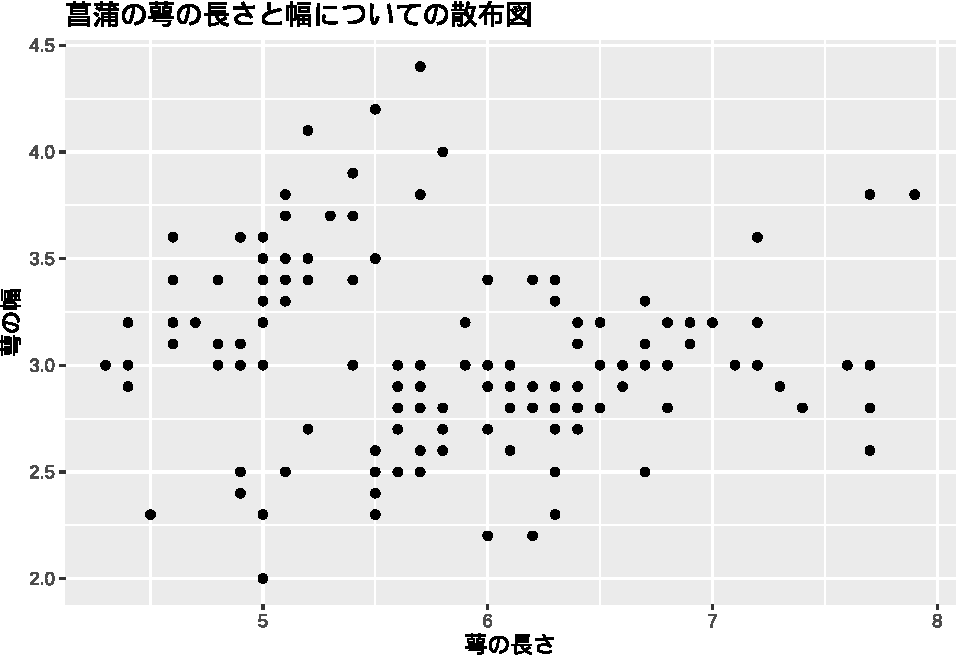
\includegraphics{31-worldbank_files/figure-latex/unnamed-chunk-8-1.pdf}

\begin{Shaded}
\begin{Highlighting}[]
\FunctionTok{WDI}\NormalTok{(}\AttributeTok{country =} \FunctionTok{c}\NormalTok{(}\StringTok{"CN"}\NormalTok{,}\StringTok{"IN"}\NormalTok{,}\StringTok{"JP"}\NormalTok{,}\StringTok{"US"}\NormalTok{), }
    \AttributeTok{indicator =} \FunctionTok{c}\NormalTok{(}\AttributeTok{gdp\_growth\_rate =} \StringTok{"NY.GDP.MKTP.KD.ZG"}\NormalTok{), }\AttributeTok{extra=}\ConstantTok{TRUE}\NormalTok{) }\SpecialCharTok{\%\textgreater{}\%}
  \FunctionTok{drop\_na}\NormalTok{(gdp\_growth\_rate) }\SpecialCharTok{\%\textgreater{}\%} 
  \FunctionTok{ggplot}\NormalTok{(}\FunctionTok{aes}\NormalTok{(year, gdp\_growth\_rate, }\AttributeTok{col =}\NormalTok{ country)) }\SpecialCharTok{+} \FunctionTok{geom\_line}\NormalTok{() }\SpecialCharTok{+}
  \FunctionTok{labs}\NormalTok{(}\AttributeTok{title =} \FunctionTok{paste}\NormalTok{(}\StringTok{"WDI NY.GDP.MKTP.KD.ZG: gdp growth rate"}\NormalTok{))}
\end{Highlighting}
\end{Shaded}

\begin{verbatim}
#> Rows: 248 Columns: 13
#> -- Column specification ------------------------------------
#> Delimiter: ","
#> chr  (7): country, iso2c, iso3c, region, capital, income...
#> dbl  (4): year, gdp_growth_rate, longitude, latitude
#> lgl  (1): status
#> date (1): lastupdated
#> 
#> i Use `spec()` to retrieve the full column specification for this data.
#> i Specify the column types or set `show_col_types = FALSE` to quiet this message.
\end{verbatim}

\includegraphics{31-worldbank_files/figure-latex/unnamed-chunk-11-1.pdf}

まず、世界の国々の、GDP(gross domestic product 国内総生産)のデータを、取得して、2021年の GDP を大きな順に並べています。

値は、たとえば、\(2.331508e+13\) のように書かれていますが、これは、科学的記法と呼ばれるもので、\(2.331508 \times 10^{13}\) を意味しています。約23兆ドルです。

次に、3兆ドル以上の、6カ国を選択し、その、iso2c と呼ばれるコードを使って、それらの国のデータをもう一度取得し、年次変化をあらわすグラフを描いています。

さらにその中から、4カ国を選んで、今度は、GDP の年次変化率を描いています。単位は、パーセントです。

これは、ひとつの例ですが、ここで使われているのが、WDI World Development Indicator というもので、世界銀行が、いくつかの指標を定めて、編纂しているものです。

\hypertarget{ux6307ux6a19-indicators-wdi}{%
\subsection{指標 Indicators (WDI)}\label{ux6307ux6a19-indicators-wdi}}

上の例では、次の二つの指標のコード Indicator Code (WDI Code) が使われました。

\begin{itemize}
\tightlist
\item
  NY.GDP.MKTP.CD: GDP (current US\$)
\item
  NY.GDP.MKTP.KD.ZG: GDP growth (annual \%)
\end{itemize}

\hypertarget{ux6307ux6a19-wdi-world-development-indicators}{%
\subsection{指標 WDI (World Development Indicators)}\label{ux6307ux6a19-wdi-world-development-indicators}}

\begin{quote}
The World Development Indicators is a compilation of relevant, high-quality, and internationally comparable statistics about global development and the fight against poverty. The database contains 1,400 time series indicators for 217 economies and more than 40 country groups, with data for many indicators going back more than 50 years.
\end{quote}

\begin{quote}
WDIは、世界の開発状況と、貧困との戦いに関する、適切で上質、かつ、国際的に比較可能な時系列の統計データを編纂したものです。このデータベースは、217の経済と40以上の国グループについて1,400の時系列指標を含み、指標のデータの多くは50年以上前に遡ることができます。
\end{quote}

\begin{itemize}
\tightlist
\item
  世界銀行(World Bank): \url{https://www.worldbank.org}
\item
  World Bank Open Data: \url{https://data.worldbank.org}

  \begin{itemize}
  \tightlist
  \item
    Country / Indicator \textgreater{} Featured \& All \textgreater{} Details
  \end{itemize}
\item
  \href{https://datatopics.worldbank.org/world-development-indicators/}{World Development Indicators (WDI)} :

  \begin{itemize}
  \tightlist
  \item
    Themes: Poverty and Inequality, People, Environment, Economy, States and Markets, Global Links
  \item
    Open Data \& DataBank: Explore data, Query database
  \end{itemize}
\end{itemize}

\hypertarget{ux6307ux6a19-ux306eux30b3ux30fcux30c9wdi-code-ux3092ux63a2ux3057ux3066ux307fux3088ux3046}{%
\subsection{指標 のコード、WDI code を探してみよう}\label{ux6307ux6a19-ux306eux30b3ux30fcux30c9wdi-code-ux3092ux63a2ux3057ux3066ux307fux3088ux3046}}

いくつかの探し方があります。まず、ここでは、World Bank のサイトから探す方法を説明しましょう。

ふた通りあります。

\begin{enumerate}
\def\labelenumi{\arabic{enumi}.}
\item
  \href{https://data.worldbank.org}{World Bank Open Data} にいくと、表題の下の検索窓の下に、 Country / Indicator とありますから、Indicator を選択します。すると、そこに、項目のリストが、Featured と All という二つのタブに分かれて出ています。かなり膨大です。それを選択すると、その項目のサイトに行きます。それが、指標のサイトです。図などの、右上に、Details とありますから、それを選択すると、その中に、Indicator が書かれています。 実は、指標のサイトのアドレス(URL)を見ると、そこにも、この Indicator が書かれていることがわかります。
\item
  \href{https://datatopics.worldbank.org/world-development-indicators/}{World Development Indicators (WDI)} にいくと、下のようなテーマに分かれています。
\end{enumerate}

Themes: Poverty and Inequality, People, Environment, Economy, States and Markets, Global Links

その中から、選択して、スクロールすると、そこに、指標が書かれています。

Indicator, Code, Time coverage, Region coverage, Get data

とあり、Code が、指標のコードです。実は、すべての年や、すべての地域のデータが揃っているわけではないので、この情報を見ておくことはとても重要です。ほとんど、データがない場合もあります。

一番右端の Get data からは、CSV や、データバンク(Data Bank)へのリンクがあります。

それぞれの方法で、上で使った、二つの指標およびそのコードは見つかりましたか。

1 の方法の途中に出てきた、検索窓から検索することも可能です。

\hypertarget{ux6307ux6a19-wdiux306eux4f8b}{%
\subsection{指標 WDIの例}\label{ux6307ux6a19-wdiux306eux4f8b}}

このあとの、例で使う指標を書いておきます。

\begin{itemize}
\tightlist
\item
  NY.GDP.MKTP.CD: GDP (current US\$)
\item
  NY.GDP.DEFL.KD.ZG: Inflation, GDP deflator (annual \%)
\item
  SL.UEM.TOTL.NE.ZS: Unemployment, total (\% of total labor force) (national estimate)
\item
  CPTOTNSXN: CPI Price, nominal
\item
  SL.TLF.CACT.MA.NE.ZS: Labor force participation rate, male (\% of male population ages 15+) (national estimate)
\item
  SL.TLF.CACT.FE.NE.ZS: Labor force participation rate, female (\% of male population ages 15+) (national estimate)
\end{itemize}

\hypertarget{ux7df4ux7fd2-1.---ux8abfux3079ux3066ux307fux305fux3044-wdi-ux6307ux6a19ux3068ux305dux306eux30b3ux30fcux30c9}{%
\subsection{練習 1. - 調べてみたい WDI 指標とそのコード}\label{ux7df4ux7fd2-1.---ux8abfux3079ux3066ux307fux305fux3044-wdi-ux6307ux6a19ux3068ux305dux306eux30b3ux30fcux30c9}}

いくつか、リストしてみましょう。

\hypertarget{wdi-ux30d1ux30c3ux30b1ux30fcux30b8}{%
\section{WDI パッケージ}\label{wdi-ux30d1ux30c3ux30b1ux30fcux30b8}}

\texttt{WDI} パッケージ の使い方を紹介します。

\texttt{WDI} パッケージで、データをダウンロードしたり、探したり、詳細情報を得たりできます。

\hypertarget{ux6307ux6a19-wdi-ux691cux7d22}{%
\subsection{指標 WDI 検索}\label{ux6307ux6a19-wdi-ux691cux7d22}}

まず、検索です。上で、サイトから調べる方法を紹介しましたが、\texttt{WDI} パッケージの、\texttt{WDIsearch} でも探すことができます。詳細は、右下の窓枠の Help タブの検索窓に、WDIsearch といれて調べて見てください。ここでは、二種類の検索方法を紹介します。

\hypertarget{ux691cux7d22ux4f8b-1wdiux540d}{%
\subsubsection{検索例 1(WDI名)}\label{ux691cux7d22ux4f8b-1wdiux540d}}

WDI 名に、ある文字列が含まれているものを検索します。検索文字列は、大文字・小文字は関係ありません。

\begin{Shaded}
\begin{Highlighting}[]
\FunctionTok{WDIsearch}\NormalTok{(}\AttributeTok{string =} \StringTok{"gdp"}\NormalTok{, }\AttributeTok{field =} \StringTok{"name"}\NormalTok{, }\AttributeTok{short =} \ConstantTok{TRUE}\NormalTok{, }\AttributeTok{cache =} \ConstantTok{NULL}\NormalTok{) }\SpecialCharTok{\%\textgreater{}\%}
  \FunctionTok{as\_tibble}\NormalTok{()}
\CommentTok{\#\textgreater{} \# A tibble: 540 x 2}
\CommentTok{\#\textgreater{}    indicator            name                                }
\CommentTok{\#\textgreater{}    \textless{}chr\textgreater{}                \textless{}chr\textgreater{}                               }
\CommentTok{\#\textgreater{}  1 5.51.01.10.gdp       "Per capita GDP growth"             }
\CommentTok{\#\textgreater{}  2 6.0.GDP\_current      "GDP (current $)"                   }
\CommentTok{\#\textgreater{}  3 6.0.GDP\_growth       "GDP growth (annual \%)"             }
\CommentTok{\#\textgreater{}  4 6.0.GDP\_usd          "GDP (constant 2005 $)"             }
\CommentTok{\#\textgreater{}  5 6.0.GDPpc\_constant   "GDP per capita, PPP (constant 2011\textasciitilde{}}
\CommentTok{\#\textgreater{}  6 BG.GSR.NFSV.GD.ZS    "Trade in services (\% of GDP)"      }
\CommentTok{\#\textgreater{}  7 BG.KAC.FNEI.GD.PP.ZS "Gross private capital flows (\% of \textasciitilde{}}
\CommentTok{\#\textgreater{}  8 BG.KAC.FNEI.GD.ZS    "Gross private capital flows (\% of \textasciitilde{}}
\CommentTok{\#\textgreater{}  9 BG.KLT.DINV.GD.PP.ZS "Gross foreign direct investment (\%\textasciitilde{}}
\CommentTok{\#\textgreater{} 10 BG.KLT.DINV.GD.ZS    "Gross foreign direct investment (\%\textasciitilde{}}
\CommentTok{\#\textgreater{} \# ... with 530 more rows}
\end{Highlighting}
\end{Shaded}

なんと、500件以上出てきました。Indicator(指標コード)と、Name(指標名)が列挙されます。すべてに、GDP という文字列が入っていることを確認できると思います。

\hypertarget{ux691cux7d22ux4f8b-2wdi}{%
\subsubsection{検索例 2(WDI)}\label{ux691cux7d22ux4f8b-2wdi}}

Indicator(指標コード)から、Name(指標名)を検索します。

\begin{Shaded}
\begin{Highlighting}[]
\FunctionTok{WDIsearch}\NormalTok{(}\AttributeTok{string =} \StringTok{"NY.GDP.MKTP.CD"}\NormalTok{, }\AttributeTok{field =} \StringTok{"indicator"}\NormalTok{, }\AttributeTok{short =} \ConstantTok{TRUE}\NormalTok{, }\AttributeTok{cache =} \ConstantTok{NULL}\NormalTok{)}
\CommentTok{\#\textgreater{}               indicator}
\CommentTok{\#\textgreater{} 11410    NY.GDP.MKTP.CD}
\CommentTok{\#\textgreater{} 11411 NY.GDP.MKTP.CD.XD}
\CommentTok{\#\textgreater{}                                             name}
\CommentTok{\#\textgreater{} 11410                          GDP (current US$)}
\CommentTok{\#\textgreater{} 11411 GDP deflator, index (2000=100; US$ series)}
\end{Highlighting}
\end{Shaded}

二件出てきました。

\hypertarget{ux7df4ux7fd2-2.---ux691cux7d22short}{%
\subsubsection{練習 2. - 検索(short)}\label{ux7df4ux7fd2-2.---ux691cux7d22short}}

名前で検索(``\,'' の間に、(なるべく簡単な)検索文字列を入れてください。)

\begin{Shaded}
\begin{Highlighting}[]
\FunctionTok{WDIsearch}\NormalTok{(}\AttributeTok{string =} \StringTok{""}\NormalTok{, }\AttributeTok{field =} \StringTok{"name"}\NormalTok{, }\AttributeTok{short =} \ConstantTok{TRUE}\NormalTok{, }\AttributeTok{cache =} \ConstantTok{NULL}\NormalTok{)}
\end{Highlighting}
\end{Shaded}

Indicator で検索(``\,'' の間に、調べたい indicator を入れてください。)

\begin{Shaded}
\begin{Highlighting}[]
\FunctionTok{WDIsearch}\NormalTok{(}\AttributeTok{string =} \StringTok{""}\NormalTok{, }\AttributeTok{field =} \StringTok{"indicator"}\NormalTok{, }\AttributeTok{short =} \ConstantTok{TRUE}\NormalTok{, }\AttributeTok{cache =} \ConstantTok{NULL}\NormalTok{)}
\end{Highlighting}
\end{Shaded}

\hypertarget{ux8a73ux3057ux3044ux60c5ux5831ux3092ux5f97ux308bux306bux306f}{%
\subsubsection{詳しい情報を得るには}\label{ux8a73ux3057ux3044ux60c5ux5831ux3092ux5f97ux308bux306bux306f}}

上では、Indicator(指標コード)と、Name(指標名)だけでしたが、Description(説明) なども得ることができます。

それには、\texttt{short\ =\ FALSE} とします。

一回一回、World Bank にアクセスして調べるのは、時間もかかりますから、Indicator と、名前などの情報をもったファイルを手元に持っておくことにします。それには、次のようにします。

\begin{Shaded}
\begin{Highlighting}[]
\NormalTok{wdi\_cache }\OtherTok{\textless{}{-}} \FunctionTok{WDIcache}\NormalTok{()}
\end{Highlighting}
\end{Shaded}

これは、series と、country の二つのデータ・フレームからなっているリストです。

右上の窓枠(pane)から、\texttt{wdi\_cache} を探して、中身を見てみましょう。三角印や、右から二番目の巻物のようなアイコンをクリックすると中身が見えます。

series には、すべての指標がリストされ、その情報が書かれています。

また、country には、それぞれについて、さまざまな情報が書かれています。これは、とても、たいせつな情報です。国名と、iso2c, iso3c のようなコードもありますし、地域(region)や、その国が、どの income level(収入の階級)に入るかも書かれています。また、国だけではなく、地域など、グループの名称も含まれています。

今後、さまざまに利用していきたいと思います。

\hypertarget{ux691cux7d22ux4f8b-3wdiux540d}{%
\subsubsection{検索例 3(WDI名)}\label{ux691cux7d22ux4f8b-3wdiux540d}}

\texttt{short\ =\ FALSE} として、検索してみましょう。文字列が入っている、指標名を検索します。

\begin{Shaded}
\begin{Highlighting}[]
\FunctionTok{WDIsearch}\NormalTok{(}\AttributeTok{string =} \StringTok{"CPI Price"}\NormalTok{, }\AttributeTok{field =} \StringTok{"name"}\NormalTok{, }\AttributeTok{short =} \ConstantTok{FALSE}\NormalTok{, }\AttributeTok{cache =}\NormalTok{ wdi\_cache)}
\CommentTok{\#\textgreater{}         indicator}
\CommentTok{\#\textgreater{} 2586    CPTOTNSXN}
\CommentTok{\#\textgreater{} 2587 CPTOTSAXMZGY}
\CommentTok{\#\textgreater{} 2588    CPTOTSAXN}
\CommentTok{\#\textgreater{} 2589 CPTOTSAXNZGY}
\CommentTok{\#\textgreater{}                                                 name}
\CommentTok{\#\textgreater{} 2586                              CPI Price, nominal}
\CommentTok{\#\textgreater{} 2587 CPI Price, \% y{-}o{-}y, median weighted, seas. adj.}
\CommentTok{\#\textgreater{} 2588                  CPI Price, nominal, seas. adj.}
\CommentTok{\#\textgreater{} 2589         CPI Price, \% y{-}o{-}y, nominal, seas. adj.}
\CommentTok{\#\textgreater{}                                                                                                                                                                                                                  description}
\CommentTok{\#\textgreater{} 2586                                                                The consumer price index reflects the change in prices for the average consumer of a constant basket of consumer goods. Data is not seasonally adjusted.}
\CommentTok{\#\textgreater{} 2587                                                                Median inflation rate calculated for geographical aggregates (regions, world, etc) of the annual percent change of the CPI. Data is seasonally adjusted.}
\CommentTok{\#\textgreater{} 2588                                               The consumer price index reflects the change in prices for the average consumer of a constant basket of consumer goods. Data is in nominal terms and seasonally adjusted.}
\CommentTok{\#\textgreater{} 2589 The consumer price index reflects the change in prices for the average consumer of a constant basket of consumer goods. Data is in nominal percentage terms, measured on a year{-}on{-}year basis, and seasonally adjusted.}
\CommentTok{\#\textgreater{}               sourceDatabase}
\CommentTok{\#\textgreater{} 2586 Global Economic Monitor}
\CommentTok{\#\textgreater{} 2587 Global Economic Monitor}
\CommentTok{\#\textgreater{} 2588 Global Economic Monitor}
\CommentTok{\#\textgreater{} 2589 Global Economic Monitor}
\CommentTok{\#\textgreater{}                                           sourceOrganization}
\CommentTok{\#\textgreater{} 2586 World Bank staff calculations based on Datastream data.}
\CommentTok{\#\textgreater{} 2587 World Bank staff calculations based on Datastream data.}
\CommentTok{\#\textgreater{} 2588 World Bank staff calculations based on Datastream data.}
\CommentTok{\#\textgreater{} 2589 World Bank staff calculations based on Datastream data.}
\end{Highlighting}
\end{Shaded}

\begin{itemize}
\tightlist
\item
  CPTOTNSXN: CPI Price, nominal

  \begin{itemize}
  \tightlist
  \item
    The consumer price index reflects the change in prices for the average consumer of a constant basket of consumer goods. Data is not seasonally adjusted.
  \end{itemize}
\end{itemize}

\hypertarget{ux691cux7d22ux4f8b-4wdi}{%
\subsubsection{検索例 4(WDI)}\label{ux691cux7d22ux4f8b-4wdi}}

指標コードから、詳細情報を得ます。

\begin{Shaded}
\begin{Highlighting}[]
\FunctionTok{WDIsearch}\NormalTok{(}\AttributeTok{string =} \StringTok{"NY.GDP.MKTP.KD.ZG"}\NormalTok{, }\AttributeTok{field =} \StringTok{"indicator"}\NormalTok{, }\AttributeTok{short =} \ConstantTok{FALSE}\NormalTok{, }\AttributeTok{cache =}\NormalTok{ wdi\_cache)}
\CommentTok{\#\textgreater{}               indicator                  name}
\CommentTok{\#\textgreater{} 12114 NY.GDP.MKTP.KD.ZG GDP growth (annual \%)}
\CommentTok{\#\textgreater{}                                                                                                                                                                                                                                                                                                                                                                                                                                                                           description}
\CommentTok{\#\textgreater{} 12114 Annual percentage growth rate of GDP at market prices based on constant local currency. Aggregates are based on constant 2015 prices, expressed in U.S. dollars. GDP is the sum of gross value added by all resident producers in the economy plus any product taxes and minus any subsidies not included in the value of the products. It is calculated without making deductions for depreciation of fabricated assets or for depletion and degradation of natural resources.}
\CommentTok{\#\textgreater{}                     sourceDatabase}
\CommentTok{\#\textgreater{} 12114 World Development Indicators}
\CommentTok{\#\textgreater{}                                                              sourceOrganization}
\CommentTok{\#\textgreater{} 12114 World Bank national accounts data, and OECD National Accounts data files.}
\end{Highlighting}
\end{Shaded}

\hypertarget{ux7df4ux7fd2-2---ux691cux7d22long-w-cache}{%
\subsubsection{練習 2 - 検索(long w/ cache)}\label{ux7df4ux7fd2-2---ux691cux7d22long-w-cache}}

\texttt{string} と、\texttt{field} を、ふたつとも入れてください。

\begin{Shaded}
\begin{Highlighting}[]
\FunctionTok{WDIsearch}\NormalTok{(}\AttributeTok{string =} \StringTok{""}\NormalTok{, }\AttributeTok{field =} \StringTok{""}\NormalTok{, }\AttributeTok{short =} \ConstantTok{FALSE}\NormalTok{, }\AttributeTok{cache =}\NormalTok{ wdi\_cache)}
\end{Highlighting}
\end{Shaded}

\hypertarget{ux6307ux6a19-wdi-ux30c7ux30fcux30bfux306eux30c0ux30a6ux30f3ux30edux30fcux30c9}{%
\subsection{指標 WDI データのダウンロード}\label{ux6307ux6a19-wdi-ux30c7ux30fcux30bfux306eux30c0ux30a6ux30f3ux30edux30fcux30c9}}

Indicator が決まったら、ダウンロードします。右下の窓枠の Help タブの検索枠に、\texttt{WDI} と入れて確認しましょう。

\begin{verbatim}
WDI(
  country = "all",
  indicator = "NY.GDP.PCAP.KD",
  start = 1960,
  end = NULL,
  extra = FALSE,
  cache = NULL,
  latest = NULL,
  language = "en"
)
\end{verbatim}

上が基本的な用法ですが、\texttt{start} 以下は、Default(初期値)が書かれていますから、たいせつなのは、最初の二つ、country と、indicator です。

\hypertarget{ux30c0ux30a6ux30f3ux30edux30fcux30c9ux4f8b-1-1}{%
\subsubsection{ダウンロード例 1-1}\label{ux30c0ux30a6ux30f3ux30edux30fcux30c9ux4f8b-1-1}}

country は、初期値も、``all'' となっていますから、最も簡単なのは、indicator に、指標コードを入れることです。引用符を忘れずに。

\begin{Shaded}
\begin{Highlighting}[]
\NormalTok{df\_gdp1 }\OtherTok{\textless{}{-}} \FunctionTok{WDI}\NormalTok{(}\AttributeTok{country =} \StringTok{"all"}\NormalTok{, }\AttributeTok{indicator =} \StringTok{"NY.GDP.MKTP.CD"}\NormalTok{)}
\NormalTok{df\_gdp1}
\end{Highlighting}
\end{Shaded}

\begin{verbatim}
#> Rows: 16492 Columns: 5
#> -- Column specification ------------------------------------
#> Delimiter: ","
#> chr (3): country, iso2c, iso3c
#> dbl (2): year, NY.GDP.MKTP.CD
#> 
#> i Use `spec()` to retrieve the full column specification for this data.
#> i Specify the column types or set `show_col_types = FALSE` to quiet this message.
#> # A tibble: 16,492 x 5
#>    country                  iso2c iso3c  year NY.GDP.MKTP.CD
#>    <chr>                    <chr> <chr> <dbl>          <dbl>
#>  1 Africa Eastern and Sout~ ZH    AFE    2021        1.08e12
#>  2 Africa Eastern and Sout~ ZH    AFE    2020        9.27e11
#>  3 Africa Eastern and Sout~ ZH    AFE    2019        1.00e12
#>  4 Africa Eastern and Sout~ ZH    AFE    2018        1.01e12
#>  5 Africa Eastern and Sout~ ZH    AFE    2017        1.02e12
#>  6 Africa Eastern and Sout~ ZH    AFE    2016        8.83e11
#>  7 Africa Eastern and Sout~ ZH    AFE    2015        9.25e11
#>  8 Africa Eastern and Sout~ ZH    AFE    2014        1.00e12
#>  9 Africa Eastern and Sout~ ZH    AFE    2013        9.83e11
#> 10 Africa Eastern and Sout~ ZH    AFE    2012        9.73e11
#> # i 16,482 more rows
\end{verbatim}

これでも良いのですが、利用するには、指標コードではわかりにくいので、それを簡単な名前に置き換えて、データを読み込むこができます。

\hypertarget{ux30c0ux30a6ux30f3ux30edux30fcux30c9ux4f8b-1-2}{%
\subsubsection{ダウンロード例 1-2}\label{ux30c0ux30a6ux30f3ux30edux30fcux30c9ux4f8b-1-2}}

\begin{Shaded}
\begin{Highlighting}[]
\NormalTok{df\_gdp2 }\OtherTok{\textless{}{-}} \FunctionTok{WDI}\NormalTok{(}\AttributeTok{country =} \StringTok{"all"}\NormalTok{, }\AttributeTok{indicator =} \FunctionTok{c}\NormalTok{(}\AttributeTok{gdp =} \StringTok{"NY.GDP.MKTP.CD"}\NormalTok{))}
\NormalTok{df\_gdp2}
\end{Highlighting}
\end{Shaded}

\begin{verbatim}
#> Rows: 16492 Columns: 5
#> -- Column specification ------------------------------------
#> Delimiter: ","
#> chr (3): country, iso2c, iso3c
#> dbl (2): year, gdp
#> 
#> i Use `spec()` to retrieve the full column specification for this data.
#> i Specify the column types or set `show_col_types = FALSE` to quiet this message.
#> # A tibble: 16,492 x 5
#>    country                     iso2c iso3c  year     gdp
#>    <chr>                       <chr> <chr> <dbl>   <dbl>
#>  1 Africa Eastern and Southern ZH    AFE    2021 1.08e12
#>  2 Africa Eastern and Southern ZH    AFE    2020 9.27e11
#>  3 Africa Eastern and Southern ZH    AFE    2019 1.00e12
#>  4 Africa Eastern and Southern ZH    AFE    2018 1.01e12
#>  5 Africa Eastern and Southern ZH    AFE    2017 1.02e12
#>  6 Africa Eastern and Southern ZH    AFE    2016 8.83e11
#>  7 Africa Eastern and Southern ZH    AFE    2015 9.25e11
#>  8 Africa Eastern and Southern ZH    AFE    2014 1.00e12
#>  9 Africa Eastern and Southern ZH    AFE    2013 9.83e11
#> 10 Africa Eastern and Southern ZH    AFE    2012 9.73e11
#> # i 16,482 more rows
\end{verbatim}

\hypertarget{ux30c0ux30a6ux30f3ux30edux30fcux30c9ux4f8b-1-3}{%
\subsubsection{\texorpdfstring{ダウンロード例 1-3\\
}{ダウンロード例 1-3 }}\label{ux30c0ux30a6ux30f3ux30edux30fcux30c9ux4f8b-1-3}}

今度は、\texttt{extra\ =\ TRUE} として、読み込みましょう。先ほど、読み込んである、\texttt{wdi\_cache} を使います。

\begin{Shaded}
\begin{Highlighting}[]
\NormalTok{df\_gdp3 }\OtherTok{\textless{}{-}} \FunctionTok{WDI}\NormalTok{(}\AttributeTok{country =} \StringTok{"all"}\NormalTok{, }\AttributeTok{indicator =} \FunctionTok{c}\NormalTok{(}\AttributeTok{gdp =} \StringTok{"NY.GDP.MKTP.CD"}\NormalTok{), }
               \AttributeTok{extra=}\ConstantTok{TRUE}\NormalTok{, }\AttributeTok{cache=}\NormalTok{wdi\_cache)}
\NormalTok{df\_gdp3}
\end{Highlighting}
\end{Shaded}

\begin{verbatim}
#> Rows: 16492 Columns: 13
#> -- Column specification ------------------------------------
#> Delimiter: ","
#> chr  (7): country, iso2c, iso3c, region, capital, income...
#> dbl  (4): year, gdp, longitude, latitude
#> lgl  (1): status
#> date (1): lastupdated
#> 
#> i Use `spec()` to retrieve the full column specification for this data.
#> i Specify the column types or set `show_col_types = FALSE` to quiet this message.
#> # A tibble: 16,492 x 13
#>    country     iso2c iso3c  year      gdp status lastupdated
#>    <chr>       <chr> <chr> <dbl>    <dbl> <lgl>  <date>     
#>  1 Afghanistan AF    AFG    2021  1.48e10 NA     2022-12-22 
#>  2 Afghanistan AF    AFG    2020  2.01e10 NA     2022-12-22 
#>  3 Afghanistan AF    AFG    2019  1.89e10 NA     2022-12-22 
#>  4 Afghanistan AF    AFG    2018  1.84e10 NA     2022-12-22 
#>  5 Afghanistan AF    AFG    2017  1.89e10 NA     2022-12-22 
#>  6 Afghanistan AF    AFG    2016  1.80e10 NA     2022-12-22 
#>  7 Afghanistan AF    AFG    2015  2.00e10 NA     2022-12-22 
#>  8 Afghanistan AF    AFG    2014  2.06e10 NA     2022-12-22 
#>  9 Afghanistan AF    AFG    2013  2.06e10 NA     2022-12-22 
#> 10 Afghanistan AF    AFG    2012  2.02e10 NA     2022-12-22 
#> # i 16,482 more rows
#> # i 6 more variables: region <chr>, capital <chr>,
#> #   longitude <dbl>, latitude <dbl>, income <chr>,
#> #   lending <chr>
\end{verbatim}

右上の三角印を使って、どのような詳細情報が付加されたか見て見ましょう。どんなことがわかりますか。

\hypertarget{ux30c0ux30a6ux30f3ux30edux30fcux30c9ux4f8b-1-4}{%
\subsubsection{ダウンロード例 1-4}\label{ux30c0ux30a6ux30f3ux30edux30fcux30c9ux4f8b-1-4}}

国名を指定します。\texttt{WDI} では、iso2c コードを使って、国名を指定します。上で見たように、Envoronment から、\texttt{wdi\_cache} を選択すると、国名と、iso2c コード両方を見ることができました。iso2c や、iso3c は、よく使われるので、web 検索でも簡単にみつけることができます。最初に紹介した例ですから、どの国かはわかりますね、

\begin{Shaded}
\begin{Highlighting}[]
\NormalTok{df\_gdp4 }\OtherTok{\textless{}{-}} \FunctionTok{WDI}\NormalTok{(}\AttributeTok{country =} \FunctionTok{c}\NormalTok{(}\StringTok{"CN"}\NormalTok{,}\StringTok{"GB"}\NormalTok{,}\StringTok{"JP"}\NormalTok{,}\StringTok{"IN"}\NormalTok{,}\StringTok{"US"}\NormalTok{,}\StringTok{"DE"}\NormalTok{), }
               \AttributeTok{indicator =} \FunctionTok{c}\NormalTok{(}\AttributeTok{gdp =} \StringTok{"NY.GDP.MKTP.CD"}\NormalTok{), }\AttributeTok{extra=}\ConstantTok{TRUE}\NormalTok{, }\AttributeTok{cache=}\NormalTok{wdi\_cache)}
\NormalTok{df\_gdp4}
\end{Highlighting}
\end{Shaded}

\begin{verbatim}
#> Rows: 372 Columns: 13
#> -- Column specification ------------------------------------
#> Delimiter: ","
#> chr  (7): country, iso2c, iso3c, region, capital, income...
#> dbl  (4): year, gdp, longitude, latitude
#> lgl  (1): status
#> date (1): lastupdated
#> 
#> i Use `spec()` to retrieve the full column specification for this data.
#> i Specify the column types or set `show_col_types = FALSE` to quiet this message.
#> # A tibble: 372 x 13
#>    country iso2c iso3c  year     gdp status lastupdated
#>    <chr>   <chr> <chr> <dbl>   <dbl> <lgl>  <date>     
#>  1 China   CN    CHN    2021 1.77e13 NA     2022-12-22 
#>  2 China   CN    CHN    2020 1.47e13 NA     2022-12-22 
#>  3 China   CN    CHN    2019 1.43e13 NA     2022-12-22 
#>  4 China   CN    CHN    2018 1.39e13 NA     2022-12-22 
#>  5 China   CN    CHN    2017 1.23e13 NA     2022-12-22 
#>  6 China   CN    CHN    2016 1.12e13 NA     2022-12-22 
#>  7 China   CN    CHN    2015 1.11e13 NA     2022-12-22 
#>  8 China   CN    CHN    2014 1.05e13 NA     2022-12-22 
#>  9 China   CN    CHN    2013 9.57e12 NA     2022-12-22 
#> 10 China   CN    CHN    2012 8.53e12 NA     2022-12-22 
#> # i 362 more rows
#> # i 6 more variables: region <chr>, capital <chr>,
#> #   longitude <dbl>, latitude <dbl>, income <chr>,
#> #   lending <chr>
\end{verbatim}

\hypertarget{ux30c0ux30a6ux30f3ux30edux30fcux30c9ux4f8b-2-1}{%
\subsubsection{ダウンロード例 2-1}\label{ux30c0ux30a6ux30f3ux30edux30fcux30c9ux4f8b-2-1}}

二つの、指標コードを使って、同時に読み込むこともできます。そのときは、\texttt{c()} (combine) を使います。

\begin{itemize}
\tightlist
\item
  NY.GDP.DEFL.KD.ZG: Inflation, GDP deflator (annual \%)
\item
  CPTOTNSXN: CPI Price, nominal
\end{itemize}

\begin{Shaded}
\begin{Highlighting}[]
\NormalTok{df\_gdp21 }\OtherTok{\textless{}{-}} \FunctionTok{WDI}\NormalTok{(}\AttributeTok{country =} \StringTok{"all"}\NormalTok{, }
                \AttributeTok{indicator =} \FunctionTok{c}\NormalTok{(}\AttributeTok{gdp\_deflator =} \StringTok{"NY.GDP.DEFL.KD.ZG"}\NormalTok{, }
                              \AttributeTok{cpi\_price =} \StringTok{"CPTOTNSXN"}\NormalTok{), }
                \AttributeTok{extra=}\ConstantTok{TRUE}\NormalTok{, }\AttributeTok{cache=}\NormalTok{wdi\_cache)}
\NormalTok{df\_gdp21}
\end{Highlighting}
\end{Shaded}

\begin{verbatim}
#> Rows: 23972 Columns: 14
#> -- Column specification ------------------------------------
#> Delimiter: ","
#> chr  (7): country, iso2c, iso3c, region, capital, income...
#> dbl  (5): year, gdp_deflator, cpi_price, longitude, lati...
#> lgl  (1): status
#> date (1): lastupdated
#> 
#> i Use `spec()` to retrieve the full column specification for this data.
#> i Specify the column types or set `show_col_types = FALSE` to quiet this message.
#> # A tibble: 23,972 x 14
#>    country iso2c iso3c  year status lastupdated gdp_deflator
#>    <chr>   <chr> <chr> <dbl> <lgl>  <date>             <dbl>
#>  1 Advanc~ AME   <NA>   1987 NA     2020-07-27            NA
#>  2 Advanc~ AME   <NA>   1988 NA     2020-07-27            NA
#>  3 Advanc~ AME   <NA>   1989 NA     2020-07-27            NA
#>  4 Advanc~ AME   <NA>   1990 NA     2020-07-27            NA
#>  5 Advanc~ AME   <NA>   1991 NA     2020-07-27            NA
#>  6 Advanc~ AME   <NA>   1992 NA     2020-07-27            NA
#>  7 Advanc~ AME   <NA>   1993 NA     2020-07-27            NA
#>  8 Advanc~ AME   <NA>   1994 NA     2020-07-27            NA
#>  9 Advanc~ AME   <NA>   1995 NA     2020-07-27            NA
#> 10 Advanc~ AME   <NA>   1996 NA     2020-07-27            NA
#> # i 23,962 more rows
#> # i 7 more variables: cpi_price <dbl>, region <chr>,
#> #   capital <chr>, longitude <dbl>, latitude <dbl>,
#> #   income <chr>, lending <chr>
\end{verbatim}

NA (not available) つまり、データがないものが多いことがわかります。もう少し、データをよく見て見ましょう。

\begin{Shaded}
\begin{Highlighting}[]
\FunctionTok{str}\NormalTok{(df\_gdp21)}
\CommentTok{\#\textgreater{} spc\_tbl\_ [23,972 x 14] (S3: spec\_tbl\_df/tbl\_df/tbl/data.frame)}
\CommentTok{\#\textgreater{}  $ country     : chr [1:23972] "Advanced Economies" "Advanced Economies" "Advanced Economies" "Advanced Economies" ...}
\CommentTok{\#\textgreater{}  $ iso2c       : chr [1:23972] "AME" "AME" "AME" "AME" ...}
\CommentTok{\#\textgreater{}  $ iso3c       : chr [1:23972] NA NA NA NA ...}
\CommentTok{\#\textgreater{}  $ year        : num [1:23972] 1987 1988 1989 1990 1991 ...}
\CommentTok{\#\textgreater{}  $ status      : logi [1:23972] NA NA NA NA NA NA ...}
\CommentTok{\#\textgreater{}  $ lastupdated : Date[1:23972], format: "2020{-}07{-}27" ...}
\CommentTok{\#\textgreater{}  $ gdp\_deflator: num [1:23972] NA NA NA NA NA NA NA NA NA NA ...}
\CommentTok{\#\textgreater{}  $ cpi\_price   : num [1:23972] 58.7 60.5 63 66 69.1 ...}
\CommentTok{\#\textgreater{}  $ region      : chr [1:23972] NA NA NA NA ...}
\CommentTok{\#\textgreater{}  $ capital     : chr [1:23972] NA NA NA NA ...}
\CommentTok{\#\textgreater{}  $ longitude   : num [1:23972] NA NA NA NA NA NA NA NA NA NA ...}
\CommentTok{\#\textgreater{}  $ latitude    : num [1:23972] NA NA NA NA NA NA NA NA NA NA ...}
\CommentTok{\#\textgreater{}  $ income      : chr [1:23972] NA NA NA NA ...}
\CommentTok{\#\textgreater{}  $ lending     : chr [1:23972] NA NA NA NA ...}
\CommentTok{\#\textgreater{}  {-} attr(*, "spec")=}
\CommentTok{\#\textgreater{}   .. cols(}
\CommentTok{\#\textgreater{}   ..   country = col\_character(),}
\CommentTok{\#\textgreater{}   ..   iso2c = col\_character(),}
\CommentTok{\#\textgreater{}   ..   iso3c = col\_character(),}
\CommentTok{\#\textgreater{}   ..   year = col\_double(),}
\CommentTok{\#\textgreater{}   ..   status = col\_logical(),}
\CommentTok{\#\textgreater{}   ..   lastupdated = col\_date(format = ""),}
\CommentTok{\#\textgreater{}   ..   gdp\_deflator = col\_double(),}
\CommentTok{\#\textgreater{}   ..   cpi\_price = col\_double(),}
\CommentTok{\#\textgreater{}   ..   region = col\_character(),}
\CommentTok{\#\textgreater{}   ..   capital = col\_character(),}
\CommentTok{\#\textgreater{}   ..   longitude = col\_double(),}
\CommentTok{\#\textgreater{}   ..   latitude = col\_double(),}
\CommentTok{\#\textgreater{}   ..   income = col\_character(),}
\CommentTok{\#\textgreater{}   ..   lending = col\_character()}
\CommentTok{\#\textgreater{}   .. )}
\CommentTok{\#\textgreater{}  {-} attr(*, "problems")=\textless{}externalptr\textgreater{}}
\end{Highlighting}
\end{Shaded}

\begin{Shaded}
\begin{Highlighting}[]
\FunctionTok{summary}\NormalTok{(df\_gdp21)}
\CommentTok{\#\textgreater{}    country             iso2c              iso3c          }
\CommentTok{\#\textgreater{}  Length:23972       Length:23972       Length:23972      }
\CommentTok{\#\textgreater{}  Class :character   Class :character   Class :character  }
\CommentTok{\#\textgreater{}  Mode  :character   Mode  :character   Mode  :character  }
\CommentTok{\#\textgreater{}                                                          }
\CommentTok{\#\textgreater{}                                                          }
\CommentTok{\#\textgreater{}                                                          }
\CommentTok{\#\textgreater{}                                                          }
\CommentTok{\#\textgreater{}       year       status         lastupdated        }
\CommentTok{\#\textgreater{}  Min.   :1960   Mode:logical   Min.   :2020{-}07{-}27  }
\CommentTok{\#\textgreater{}  1st Qu.:1982   NA\textquotesingle{}s:23972     1st Qu.:2020{-}07{-}27  }
\CommentTok{\#\textgreater{}  Median :1996                  Median :2022{-}12{-}22  }
\CommentTok{\#\textgreater{}  Mean   :1995                  Mean   :2022{-}03{-}23  }
\CommentTok{\#\textgreater{}  3rd Qu.:2009                  3rd Qu.:2022{-}12{-}22  }
\CommentTok{\#\textgreater{}  Max.   :2021                  Max.   :2022{-}12{-}22  }
\CommentTok{\#\textgreater{}                                                    }
\CommentTok{\#\textgreater{}   gdp\_deflator         cpi\_price         region         }
\CommentTok{\#\textgreater{}  Min.   :  {-}98.704   Min.   :  0.00   Length:23972      }
\CommentTok{\#\textgreater{}  1st Qu.:    2.317   1st Qu.: 55.95   Class :character  }
\CommentTok{\#\textgreater{}  Median :    5.273   Median : 83.28   Mode  :character  }
\CommentTok{\#\textgreater{}  Mean   :   25.308   Mean   : 84.18                     }
\CommentTok{\#\textgreater{}  3rd Qu.:   10.411   3rd Qu.:108.75                     }
\CommentTok{\#\textgreater{}  Max.   :26765.858   Max.   :551.25                     }
\CommentTok{\#\textgreater{}  NA\textquotesingle{}s   :11616       NA\textquotesingle{}s   :18410                      }
\CommentTok{\#\textgreater{}    capital            longitude          latitude      }
\CommentTok{\#\textgreater{}  Length:23972       Min.   :{-}175.22   Min.   :{-}41.286  }
\CommentTok{\#\textgreater{}  Class :character   1st Qu.: {-}15.18   1st Qu.:  4.174  }
\CommentTok{\#\textgreater{}  Mode  :character   Median :  19.26   Median : 17.300  }
\CommentTok{\#\textgreater{}                     Mean   :  19.14   Mean   : 18.889  }
\CommentTok{\#\textgreater{}                     3rd Qu.:  50.53   3rd Qu.: 40.050  }
\CommentTok{\#\textgreater{}                     Max.   : 179.09   Max.   : 64.184  }
\CommentTok{\#\textgreater{}                     NA\textquotesingle{}s   :10890     NA\textquotesingle{}s   :10890    }
\CommentTok{\#\textgreater{}     income            lending         }
\CommentTok{\#\textgreater{}  Length:23972       Length:23972      }
\CommentTok{\#\textgreater{}  Class :character   Class :character  }
\CommentTok{\#\textgreater{}  Mode  :character   Mode  :character  }
\CommentTok{\#\textgreater{}                                       }
\CommentTok{\#\textgreater{}                                       }
\CommentTok{\#\textgreater{}                                       }
\CommentTok{\#\textgreater{} }
\end{Highlighting}
\end{Shaded}

どんなことが分かりましたか。

右上の窓枠の、Environment でも \texttt{df\_gdp21} を見てみましょう。

\hypertarget{ux53efux8996ux5316-visualization}{%
\section{可視化 Visualization}\label{ux53efux8996ux5316-visualization}}

グラフ(Chart)を描いて視覚化します。ここでは、年ごとの変化をみる、折れ線グラフだけを描いて見ます。

\hypertarget{ux30b0ux30e9ux30d5-1}{%
\subsection{グラフ 1}\label{ux30b0ux30e9ux30d5-1}}

\texttt{x\ =\ year}, \texttt{y\ =\ gdp} の、\texttt{x=}, \texttt{y=} は省略してあります。\texttt{col=country} は、国ごとに、グループにして、色分けをします。\texttt{col} は、\texttt{color} としても \texttt{colour} としても、問題ありません。 `

\begin{Shaded}
\begin{Highlighting}[]
\NormalTok{df\_gdp4 }\SpecialCharTok{\%\textgreater{}\%} \FunctionTok{ggplot}\NormalTok{(}\FunctionTok{aes}\NormalTok{(year, gdp, }\AttributeTok{col=}\NormalTok{country)) }\SpecialCharTok{+} \FunctionTok{geom\_line}\NormalTok{()}
\CommentTok{\#\textgreater{} Warning: Removed 10 rows containing missing values}
\CommentTok{\#\textgreater{} (\textasciigrave{}geom\_line()\textasciigrave{}).}
\end{Highlighting}
\end{Shaded}

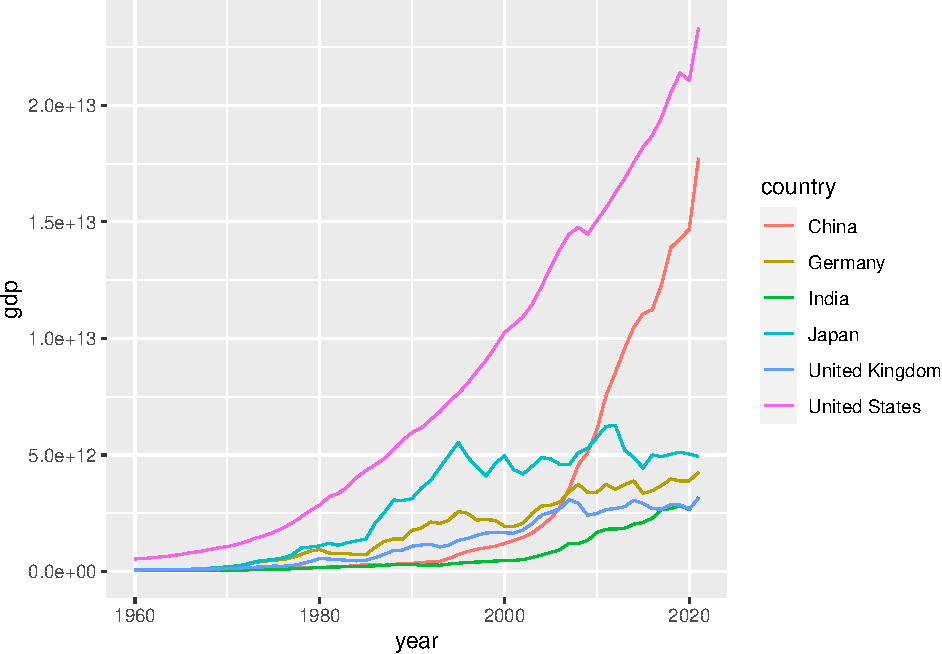
\includegraphics{31-worldbank_files/figure-latex/unnamed-chunk-39-1.pdf}

Warning として、missing values があると出ています。どこかは、分かりませんが、図を書くときですから、\texttt{y} に対応する、\texttt{gdp} の値がないものと思われます。

\hypertarget{ux30b0ux30e9ux30d5-2}{%
\subsection{グラフ 2}\label{ux30b0ux30e9ux30d5-2}}

\texttt{drop\_na(gdp)} で、\texttt{gdp} の値が、NA であるものを削除します。また、\texttt{labs} で、図にタイトルをつけます。

\begin{Shaded}
\begin{Highlighting}[]
\NormalTok{df\_gdp4 }\SpecialCharTok{\%\textgreater{}\%} \FunctionTok{drop\_na}\NormalTok{(gdp) }\SpecialCharTok{\%\textgreater{}\%} 
  \FunctionTok{ggplot}\NormalTok{(}\FunctionTok{aes}\NormalTok{(year, gdp, }\AttributeTok{col=}\NormalTok{country)) }\SpecialCharTok{+} \FunctionTok{geom\_line}\NormalTok{() }\SpecialCharTok{+}
  \FunctionTok{labs}\NormalTok{(}\AttributeTok{title =} \StringTok{"WDI {-} NY.GDP.MKTP.CD: gdp"}\NormalTok{)}
\end{Highlighting}
\end{Shaded}

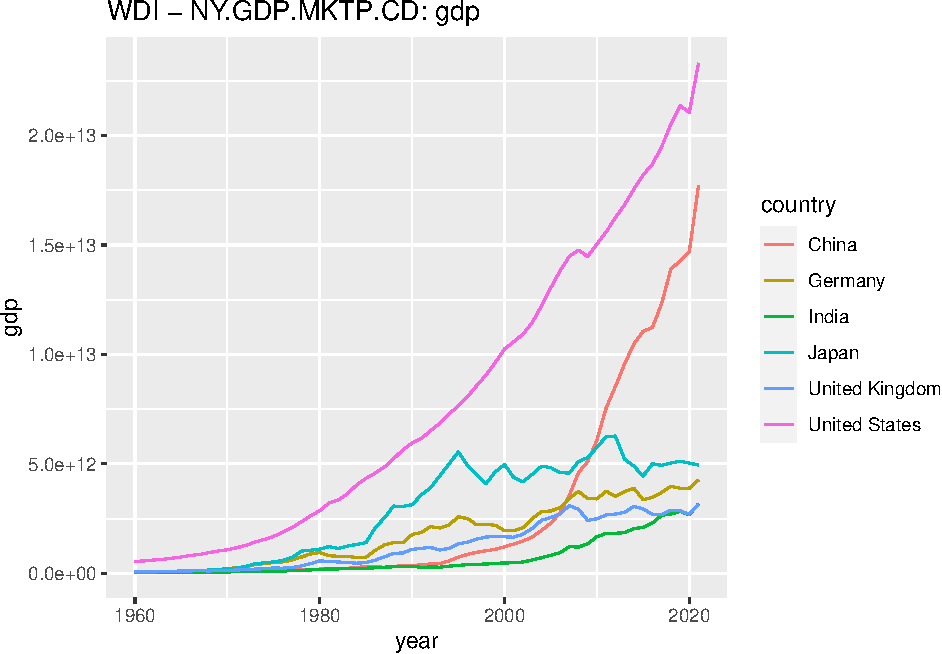
\includegraphics{31-worldbank_files/figure-latex/unnamed-chunk-40-1.pdf}

\hypertarget{ux30c6ux30f3ux30d7ux30ecux30fcux30c8-templates}{%
\subsection{テンプレート Templates}\label{ux30c6ux30f3ux30d7ux30ecux30fcux30c8-templates}}

下に、テンプレートをつけます。コピーして、指標コードや、略称、国などを、それぞれ置き換えて、試して見てください。少し、複雑な変形をしていますが、少しずつ説明します。

\hypertarget{ux4e00ux3064ux306eux56fdux306bux3064ux3044ux3066ux306eux4e00ux3064ux306eux6307ux6a19wdiux3068ux305dux306eux7565ux79f0ux304bux3089ux6298ux7ddaux30b0ux30e9ux30d5ux3092ux4f5cux6210}{%
\subsubsection{一つの国についての、一つの指標(WDI)と、その略称から、折線グラフを作成}\label{ux4e00ux3064ux306eux56fdux306bux3064ux3044ux3066ux306eux4e00ux3064ux306eux6307ux6a19wdiux3068ux305dux306eux7565ux79f0ux304bux3089ux6298ux7ddaux30b0ux30e9ux30d5ux3092ux4f5cux6210}}

Line Plot with one indicator with abbreviation and one country

\begin{Shaded}
\begin{Highlighting}[]
\NormalTok{chosen\_indicator }\OtherTok{\textless{}{-}} \StringTok{"SL.UEM.TOTL.NE.ZS"}
\NormalTok{short\_name }\OtherTok{\textless{}{-}} \StringTok{"unemployment"}
\NormalTok{chosen\_country }\OtherTok{\textless{}{-}} \StringTok{"United States"}
\FunctionTok{WDI}\NormalTok{(}\AttributeTok{country =} \StringTok{"all"}\NormalTok{, }\AttributeTok{indicator =} \FunctionTok{c}\NormalTok{(}\AttributeTok{short\_name =}\NormalTok{ chosen\_indicator), }\AttributeTok{extra=}\ConstantTok{TRUE}\NormalTok{, }\AttributeTok{cache=}\NormalTok{wdi\_cache) }\SpecialCharTok{\%\textgreater{}\%}
  \FunctionTok{filter}\NormalTok{(country }\SpecialCharTok{==}\NormalTok{ chosen\_country) }\SpecialCharTok{\%\textgreater{}\%} 
  \FunctionTok{ggplot}\NormalTok{(}\FunctionTok{aes}\NormalTok{(year, short\_name)) }\SpecialCharTok{+} \FunctionTok{geom\_line}\NormalTok{() }\SpecialCharTok{+}
  \FunctionTok{labs}\NormalTok{(}\AttributeTok{title =} \FunctionTok{paste}\NormalTok{(}\StringTok{"WDI "}\NormalTok{, chosen\_indicator, }\StringTok{": "}\NormalTok{, short\_name, }\StringTok{" {-} "}\NormalTok{, chosen\_country),}
       \AttributeTok{y =}\NormalTok{ short\_name)}
\end{Highlighting}
\end{Shaded}

\hypertarget{ux4e00ux3064ux306eux56fdux306bux3064ux3044ux3066ux306eux4e00ux3064ux306eux6307ux6a19wdiux304bux3089ux6298ux7ddaux30b0ux30e9ux30d5ux3092ux4f5cux6210}{%
\subsubsection{一つの国についての、一つの指標(WDI)から、折線グラフを作成}\label{ux4e00ux3064ux306eux56fdux306bux3064ux3044ux3066ux306eux4e00ux3064ux306eux6307ux6a19wdiux304bux3089ux6298ux7ddaux30b0ux30e9ux30d5ux3092ux4f5cux6210}}

Line Plot with one indicator and one country

\begin{Shaded}
\begin{Highlighting}[]
\NormalTok{chosen\_indicator }\OtherTok{\textless{}{-}} \StringTok{"SL.UEM.TOTL.NE.ZS"}
\NormalTok{chosen\_country }\OtherTok{\textless{}{-}} \StringTok{"United States"}
\FunctionTok{WDI}\NormalTok{(}\AttributeTok{country =} \StringTok{"all"}\NormalTok{, }\AttributeTok{indicator =} \FunctionTok{c}\NormalTok{(}\AttributeTok{chosen\_indicator =}\NormalTok{ chosen\_indicator), }
    \AttributeTok{extra=}\ConstantTok{TRUE}\NormalTok{, }\AttributeTok{cache=}\NormalTok{wdi\_cache) }\SpecialCharTok{\%\textgreater{}\%}
  \FunctionTok{filter}\NormalTok{(country }\SpecialCharTok{==}\NormalTok{ chosen\_country) }\SpecialCharTok{\%\textgreater{}\%} 
  \FunctionTok{ggplot}\NormalTok{(}\FunctionTok{aes}\NormalTok{(year, chosen\_indicator)) }\SpecialCharTok{+} \FunctionTok{geom\_line}\NormalTok{() }\SpecialCharTok{+}
  \FunctionTok{labs}\NormalTok{(}\AttributeTok{title =} \FunctionTok{paste}\NormalTok{(}\StringTok{"WDI "}\NormalTok{, chosen\_indicator, }\StringTok{" {-} "}\NormalTok{, chosen\_country), }
       \AttributeTok{y =}\NormalTok{ chosen\_indicator)}
\end{Highlighting}
\end{Shaded}

\hypertarget{ux3044ux304fux3064ux304bux306eux56fdux306bux3064ux3044ux3066ux306eux4e00ux3064ux306eux6307ux6a19wdiux3068ux305dux306eux7565ux79f0ux304bux3089ux6298ux7ddaux30b0ux30e9ux30d5ux3092ux4f5cux6210}{%
\subsubsection{いくつかの国についての、一つの指標(WDI)と、その略称から、折線グラフを作成}\label{ux3044ux304fux3064ux304bux306eux56fdux306bux3064ux3044ux3066ux306eux4e00ux3064ux306eux6307ux6a19wdiux3068ux305dux306eux7565ux79f0ux304bux3089ux6298ux7ddaux30b0ux30e9ux30d5ux3092ux4f5cux6210}}

Line Plot with one indicator with abbreviation and several countries

\begin{Shaded}
\begin{Highlighting}[]
\NormalTok{chosen\_indicator }\OtherTok{\textless{}{-}} \StringTok{"SL.UEM.TOTL.NE.ZS"}
\NormalTok{short\_name }\OtherTok{\textless{}{-}} \StringTok{"unemployment"}
\NormalTok{chosen\_countries }\OtherTok{\textless{}{-}} \FunctionTok{c}\NormalTok{(}\StringTok{"United States"}\NormalTok{,}\StringTok{"United Kingdom"}\NormalTok{, }\StringTok{"Japan"}\NormalTok{)}
\FunctionTok{WDI}\NormalTok{(}\AttributeTok{country =} \StringTok{"all"}\NormalTok{, }\AttributeTok{indicator =} \FunctionTok{c}\NormalTok{(}\AttributeTok{short\_name =}\NormalTok{ chosen\_indicator), }\AttributeTok{extra=}\ConstantTok{TRUE}\NormalTok{, }\AttributeTok{cache=}\NormalTok{wdi\_cache) }\SpecialCharTok{\%\textgreater{}\%} \FunctionTok{drop\_na}\NormalTok{(short\_name) }\SpecialCharTok{\%\textgreater{}\%} 
  \FunctionTok{filter}\NormalTok{(country }\SpecialCharTok{\%in\%}\NormalTok{ chosen\_countries) }\SpecialCharTok{\%\textgreater{}\%} 
  \FunctionTok{ggplot}\NormalTok{(}\FunctionTok{aes}\NormalTok{(year, short\_name, }\AttributeTok{col =}\NormalTok{ country)) }\SpecialCharTok{+} \FunctionTok{geom\_line}\NormalTok{() }\SpecialCharTok{+}
  \FunctionTok{labs}\NormalTok{(}\AttributeTok{title =} \FunctionTok{paste}\NormalTok{(}\StringTok{"WDI "}\NormalTok{, chosen\_indicator, }\StringTok{": "}\NormalTok{, short\_name), }\AttributeTok{y =}\NormalTok{ short\_name)}
\end{Highlighting}
\end{Shaded}

\hypertarget{ux4e00ux3064ux306eux56fdux306bux3064ux3044ux3066ux306eux4e8cux3064ux306eux6307ux6a19wdiux3068ux305dux306eux7565ux79f0ux304bux3089ux6298ux7ddaux30b0ux30e9ux30d5ux3092ux4f5cux6210}{%
\subsubsection{一つの国についての、二つの指標(WDI)と、その略称から、折線グラフを作成}\label{ux4e00ux3064ux306eux56fdux306bux3064ux3044ux3066ux306eux4e8cux3064ux306eux6307ux6a19wdiux3068ux305dux306eux7565ux79f0ux304bux3089ux6298ux7ddaux30b0ux30e9ux30d5ux3092ux4f5cux6210}}

Line Plot with two indicators with abbreviation and one country

\begin{Shaded}
\begin{Highlighting}[]
\NormalTok{chosen\_indicator\_1 }\OtherTok{\textless{}{-}} \StringTok{"NY.GDP.DEFL.KD.ZG"}
\NormalTok{short\_name\_1 }\OtherTok{\textless{}{-}} \StringTok{"gdp\_deflator"}
\NormalTok{chosen\_indicator\_2 }\OtherTok{\textless{}{-}} \StringTok{"CPTOTSAXNZGY"}
\NormalTok{short\_name\_2 }\OtherTok{\textless{}{-}} \StringTok{"cpi\_price"}
\NormalTok{chosen\_country }\OtherTok{\textless{}{-}} \StringTok{"United States"}
\FunctionTok{WDI}\NormalTok{(}\AttributeTok{country =} \StringTok{"all"}\NormalTok{, }\AttributeTok{indicator =} \FunctionTok{c}\NormalTok{(}\AttributeTok{short\_name\_1 =}\NormalTok{ chosen\_indicator\_1, }\AttributeTok{short\_name\_2 =}\NormalTok{ chosen\_indicator\_2), }\AttributeTok{extra=}\ConstantTok{TRUE}\NormalTok{, }\AttributeTok{cache=}\NormalTok{wdi\_cache) }\SpecialCharTok{\%\textgreater{}\%} 
  \FunctionTok{filter}\NormalTok{(country }\SpecialCharTok{==}\NormalTok{ chosen\_country) }\SpecialCharTok{\%\textgreater{}\%} 
  \FunctionTok{pivot\_longer}\NormalTok{(}\FunctionTok{c}\NormalTok{(short\_name\_1, short\_name\_2), }\AttributeTok{names\_to =} \StringTok{"class"}\NormalTok{, }\AttributeTok{values\_to =} \StringTok{"value"}\NormalTok{) }\SpecialCharTok{\%\textgreater{}\%} \FunctionTok{drop\_na}\NormalTok{(value) }\SpecialCharTok{\%\textgreater{}\%}
  \FunctionTok{ggplot}\NormalTok{(}\FunctionTok{aes}\NormalTok{(year, value, }\AttributeTok{col =}\NormalTok{ class)) }\SpecialCharTok{+} \FunctionTok{geom\_line}\NormalTok{() }\SpecialCharTok{+}
  \FunctionTok{labs}\NormalTok{(}\AttributeTok{title =} \FunctionTok{paste}\NormalTok{(}\StringTok{"WDI "}\NormalTok{, chosen\_indicator\_1, }\StringTok{": "}\NormalTok{, short\_name\_1, }\StringTok{"}\SpecialCharTok{\textbackslash{}n}\StringTok{"}\NormalTok{, chosen\_indicator\_2, }\StringTok{": "}\NormalTok{, short\_name\_2, }\StringTok{" {-} "}\NormalTok{, chosen\_country)) }\SpecialCharTok{+}
  \FunctionTok{scale\_color\_manual}\NormalTok{(}\AttributeTok{labels =} \FunctionTok{c}\NormalTok{(short\_name\_1, short\_name\_2), }\AttributeTok{values =}\NormalTok{ scales}\SpecialCharTok{::}\FunctionTok{hue\_pal}\NormalTok{()(}\DecValTok{2}\NormalTok{))}
\end{Highlighting}
\end{Shaded}

\begin{Shaded}
\begin{Highlighting}[]
\NormalTok{chosen\_indicator\_1 }\OtherTok{\textless{}{-}} \StringTok{"SL.TLF.CACT.MA.NE.ZS"}
\NormalTok{short\_name\_1 }\OtherTok{\textless{}{-}} \StringTok{"male"}
\NormalTok{chosen\_indicator\_2 }\OtherTok{\textless{}{-}} \StringTok{"SL.TLF.CACT.FE.NE.ZS"}
\NormalTok{short\_name\_2 }\OtherTok{\textless{}{-}} \StringTok{"female"}
\NormalTok{chosen\_country }\OtherTok{\textless{}{-}} \StringTok{"United States"}
\FunctionTok{WDI}\NormalTok{(}\AttributeTok{country =} \StringTok{"all"}\NormalTok{, }\AttributeTok{indicator =} \FunctionTok{c}\NormalTok{(}\AttributeTok{short\_name\_1 =}\NormalTok{ chosen\_indicator\_1, }\AttributeTok{short\_name\_2 =}\NormalTok{ chosen\_indicator\_2), }\AttributeTok{extra=}\ConstantTok{TRUE}\NormalTok{, }\AttributeTok{cache=}\NormalTok{wdi\_cache) }\SpecialCharTok{\%\textgreater{}\%} 
  \FunctionTok{filter}\NormalTok{(country }\SpecialCharTok{==}\NormalTok{ chosen\_country) }\SpecialCharTok{\%\textgreater{}\%} 
  \FunctionTok{pivot\_longer}\NormalTok{(}\FunctionTok{c}\NormalTok{(short\_name\_1, short\_name\_2), }\AttributeTok{names\_to =} \StringTok{"class"}\NormalTok{, }\AttributeTok{values\_to =} \StringTok{"value"}\NormalTok{) }\SpecialCharTok{\%\textgreater{}\%} \FunctionTok{drop\_na}\NormalTok{(value) }\SpecialCharTok{\%\textgreater{}\%}
  \FunctionTok{ggplot}\NormalTok{(}\FunctionTok{aes}\NormalTok{(year, value, }\AttributeTok{col =}\NormalTok{ class)) }\SpecialCharTok{+} \FunctionTok{geom\_line}\NormalTok{() }\SpecialCharTok{+}
  \FunctionTok{labs}\NormalTok{(}\AttributeTok{title =} \FunctionTok{paste}\NormalTok{(}\StringTok{"WDI "}\NormalTok{, chosen\_indicator\_1, }\StringTok{": "}\NormalTok{, short\_name\_1, }\StringTok{"}\SpecialCharTok{\textbackslash{}n}\StringTok{"}\NormalTok{, chosen\_indicator\_2, }\StringTok{": "}\NormalTok{, short\_name\_2, }\StringTok{" {-} "}\NormalTok{, chosen\_country)) }\SpecialCharTok{+}
  \FunctionTok{scale\_color\_manual}\NormalTok{(}\AttributeTok{labels =} \FunctionTok{c}\NormalTok{(short\_name\_1, short\_name\_2), }\AttributeTok{values =}\NormalTok{ scales}\SpecialCharTok{::}\FunctionTok{hue\_pal}\NormalTok{()(}\DecValTok{2}\NormalTok{))}
\end{Highlighting}
\end{Shaded}

\hypertarget{ux3044ux304fux3064ux304bux306eux56fdux306bux3064ux3044ux3066ux306eux4e8cux3064ux306eux6307ux6a19wdiux3068ux305dux306eux7565ux79f0ux304bux3089ux6298ux7ddaux30b0ux30e9ux30d5ux3092ux4f5cux6210}{%
\subsubsection{いくつかの国についての、二つの指標(WDI)と、その略称から、折線グラフを作成}\label{ux3044ux304fux3064ux304bux306eux56fdux306bux3064ux3044ux3066ux306eux4e8cux3064ux306eux6307ux6a19wdiux3068ux305dux306eux7565ux79f0ux304bux3089ux6298ux7ddaux30b0ux30e9ux30d5ux3092ux4f5cux6210}}

Line Plot with two indicators with abbreviation and several countries

\begin{Shaded}
\begin{Highlighting}[]
\NormalTok{chosen\_indicator\_1 }\OtherTok{\textless{}{-}} \StringTok{"NY.GDP.DEFL.KD.ZG"}
\NormalTok{short\_name\_1 }\OtherTok{\textless{}{-}} \StringTok{"gdp\_deflator"}
\NormalTok{chosen\_indicator\_2 }\OtherTok{\textless{}{-}} \StringTok{"CPTOTSAXNZGY"}
\NormalTok{short\_name\_2 }\OtherTok{\textless{}{-}} \StringTok{"cpi\_price"}
\NormalTok{chosen\_countries }\OtherTok{\textless{}{-}} \FunctionTok{c}\NormalTok{(}\StringTok{"United States"}\NormalTok{, }\StringTok{"France"}\NormalTok{, }\StringTok{"Japan"}\NormalTok{)}
\FunctionTok{WDI}\NormalTok{(}\AttributeTok{country =} \StringTok{"all"}\NormalTok{, }\AttributeTok{indicator =} \FunctionTok{c}\NormalTok{(}\AttributeTok{short\_name\_1 =}\NormalTok{ chosen\_indicator\_1, }\AttributeTok{short\_name\_2 =}\NormalTok{ chosen\_indicator\_2), }\AttributeTok{extra=}\ConstantTok{TRUE}\NormalTok{, }\AttributeTok{cache=}\NormalTok{wdi\_cache) }\SpecialCharTok{\%\textgreater{}\%} 
  \FunctionTok{filter}\NormalTok{(country }\SpecialCharTok{\%in\%}\NormalTok{ chosen\_countries) }\SpecialCharTok{\%\textgreater{}\%} 
  \FunctionTok{pivot\_longer}\NormalTok{(}\FunctionTok{c}\NormalTok{(short\_name\_1, short\_name\_2), }\AttributeTok{names\_to =} \StringTok{"class"}\NormalTok{, }\AttributeTok{values\_to =} \StringTok{"value"}\NormalTok{) }\SpecialCharTok{\%\textgreater{}\%} \FunctionTok{drop\_na}\NormalTok{(value) }\SpecialCharTok{\%\textgreater{}\%}
  \FunctionTok{ggplot}\NormalTok{(}\FunctionTok{aes}\NormalTok{(year, value, }\AttributeTok{linetype =}\NormalTok{ class, }\AttributeTok{col =}\NormalTok{ country)) }\SpecialCharTok{+} \FunctionTok{geom\_line}\NormalTok{() }\SpecialCharTok{+}
  \FunctionTok{labs}\NormalTok{(}\AttributeTok{title =} \FunctionTok{paste}\NormalTok{(}\StringTok{"WDI "}\NormalTok{, chosen\_indicator\_1, }\StringTok{": "}\NormalTok{, short\_name\_1, }\StringTok{"}\SpecialCharTok{\textbackslash{}n}\StringTok{"}\NormalTok{, chosen\_indicator\_2, }\StringTok{": "}\NormalTok{, short\_name\_2)) }\SpecialCharTok{+}
  \FunctionTok{scale\_linetype\_manual}\NormalTok{(}\AttributeTok{labels =} \FunctionTok{c}\NormalTok{(short\_name\_1, short\_name\_2), }\AttributeTok{values =} \FunctionTok{c}\NormalTok{(}\StringTok{"solid"}\NormalTok{, }\StringTok{"dashed"}\NormalTok{))}
\end{Highlighting}
\end{Shaded}

\begin{Shaded}
\begin{Highlighting}[]
\NormalTok{chosen\_indicator\_1 }\OtherTok{\textless{}{-}} \StringTok{"SL.TLF.CACT.MA.NE.ZS"}
\NormalTok{short\_name\_1 }\OtherTok{\textless{}{-}} \StringTok{"male"}
\NormalTok{chosen\_indicator\_2 }\OtherTok{\textless{}{-}} \StringTok{"SL.TLF.CACT.FE.NE.ZS"}
\NormalTok{short\_name\_2 }\OtherTok{\textless{}{-}} \StringTok{"female"}
\NormalTok{chosen\_countries }\OtherTok{\textless{}{-}} \FunctionTok{c}\NormalTok{(}\StringTok{"United States"}\NormalTok{, }\StringTok{"France"}\NormalTok{, }\StringTok{"Japan"}\NormalTok{)}
\FunctionTok{WDI}\NormalTok{(}\AttributeTok{country =} \StringTok{"all"}\NormalTok{, }\AttributeTok{indicator =} \FunctionTok{c}\NormalTok{(}\AttributeTok{short\_name\_1 =}\NormalTok{ chosen\_indicator\_1, }\AttributeTok{short\_name\_2 =}\NormalTok{ chosen\_indicator\_2), }\AttributeTok{extra=}\ConstantTok{TRUE}\NormalTok{, }\AttributeTok{cache=}\NormalTok{wdi\_cache) }\SpecialCharTok{\%\textgreater{}\%} 
  \FunctionTok{filter}\NormalTok{(country }\SpecialCharTok{\%in\%}\NormalTok{ chosen\_countries) }\SpecialCharTok{\%\textgreater{}\%} 
  \FunctionTok{pivot\_longer}\NormalTok{(}\FunctionTok{c}\NormalTok{(short\_name\_1, short\_name\_2), }\AttributeTok{names\_to =} \StringTok{"class"}\NormalTok{, }\AttributeTok{values\_to =} \StringTok{"value"}\NormalTok{) }\SpecialCharTok{\%\textgreater{}\%} \FunctionTok{drop\_na}\NormalTok{(value) }\SpecialCharTok{\%\textgreater{}\%}
  \FunctionTok{ggplot}\NormalTok{(}\FunctionTok{aes}\NormalTok{(year, value, }\AttributeTok{linetype =}\NormalTok{ class, }\AttributeTok{col =}\NormalTok{ country)) }\SpecialCharTok{+} \FunctionTok{geom\_line}\NormalTok{() }\SpecialCharTok{+}
  \FunctionTok{labs}\NormalTok{(}\AttributeTok{title =} \FunctionTok{paste}\NormalTok{(}\StringTok{"WDI "}\NormalTok{, chosen\_indicator\_1, }\StringTok{": "}\NormalTok{, short\_name\_1, }\StringTok{"}\SpecialCharTok{\textbackslash{}n}\StringTok{"}\NormalTok{, chosen\_indicator\_2, }\StringTok{": "}\NormalTok{, short\_name\_2)) }\SpecialCharTok{+}
  \FunctionTok{scale\_linetype\_manual}\NormalTok{(}\AttributeTok{labels =} \FunctionTok{c}\NormalTok{(short\_name\_1, short\_name\_2), }\AttributeTok{values =} \FunctionTok{c}\NormalTok{(}\StringTok{"solid"}\NormalTok{, }\StringTok{"dashed"}\NormalTok{))}
\end{Highlighting}
\end{Shaded}

\hypertarget{ux8ab2ux984c-assignment}{%
\section{課題 Assignment}\label{ux8ab2ux984c-assignment}}

上のテンプレートをコピーして、下に貼り付け、指標 \texttt{indicator} と、略称 \texttt{short\_name} と、いくつかの国名 \texttt{chosen\_countries} を、入れ替えて、試してみてください。

\hypertarget{part-part-iv-eda}{%
\part{PART IV EDA}\label{part-part-iv-eda}}

\hypertarget{intro2eda}{%
\chapter{探索的データ解析}\label{intro2eda}}

\hypertarget{ux63a2ux7d22ux7684ux30c7ux30fcux30bfux89e3ux6790-edaux3068ux306f}{%
\section{探索的データ解析 (EDA)とは}\label{ux63a2ux7d22ux7684ux30c7ux30fcux30bfux89e3ux6790-edaux3068ux306f}}

\begin{figure}
\centering
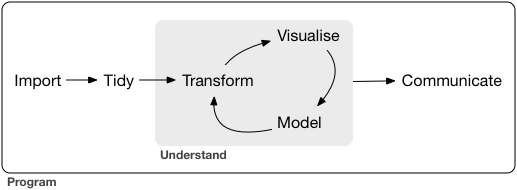
\includegraphics{./data/data-science.png}
\caption{image from r4ds}
\end{figure}

以下は、\href{https://posit.cloud/learn/primers/3.1}{Posit Primers: Visualise Data} から

探索的データ解析 (EDA) は、データを理解するための反復的なサイクルです。EDAでは、以下のことを行います。

\begin{enumerate}
\def\labelenumi{\arabic{enumi}.}
\item
  データに関する問いを作成する
\item
  データの可視化、変形・整形、モデリングによって、問いの答えを探索する。
\item
  学んだことを使って、問いをより洗練されたものとする。
\end{enumerate}

EDAは、あらゆるデータ分析において重要な役割を担います。EDA によって、課題解決のいとぐちを発見することもありますし、他の課題との関係性を発見する場合もあります。EDAを使用してデータの問題や品質を確認したり、データが信頼できるものであるかを見極める問いを作成できる場合もあります。

\hypertarget{ux63a2ux7d22ux7684ux30c7ux30fcux30bfux89e3ux6790-eda-ux306eux4e00ux4f8b}{%
\section{探索的データ解析 (EDA) の一例}\label{ux63a2ux7d22ux7684ux30c7ux30fcux30bfux89e3ux6790-eda-ux306eux4e00ux4f8b}}

WDI の一つの指標を使って、流れを見てみましょう。

\hypertarget{ux30c7ux30fcux30bfux306eux53d6ux5f97ux3068ux8aadux307fux8fbcux307f---data-import}{%
\subsection{データの取得と読み込み - Data Import}\label{ux30c7ux30fcux30bfux306eux53d6ux5f97ux3068ux8aadux307fux8fbcux307f---data-import}}

NY.GDP.PCAP.CD: GDP per capita (current US\$)

\begin{Shaded}
\begin{Highlighting}[]
\NormalTok{df\_wdi\_gdppcap }\OtherTok{\textless{}{-}} \FunctionTok{WDI}\NormalTok{(}\AttributeTok{country =} \StringTok{"all"}\NormalTok{, }\AttributeTok{indicator =} \FunctionTok{c}\NormalTok{(}\AttributeTok{gdp\_pcap =} \StringTok{"NY.GDP.PCAP.CD"}\NormalTok{))}
\FunctionTok{write\_csv}\NormalTok{(df\_wdi\_gdppcap, }\StringTok{"./data/df\_wdi\_gdppcap.csv"}\NormalTok{)}
\end{Highlighting}
\end{Shaded}

\begin{Shaded}
\begin{Highlighting}[]
\NormalTok{df\_wdi\_gdppcap}
\CommentTok{\#\textgreater{} \# A tibble: 16,492 x 5}
\CommentTok{\#\textgreater{}    country                     iso2c iso3c  year gdp\_pcap}
\CommentTok{\#\textgreater{}    \textless{}chr\textgreater{}                       \textless{}chr\textgreater{} \textless{}chr\textgreater{} \textless{}dbl\textgreater{}    \textless{}dbl\textgreater{}}
\CommentTok{\#\textgreater{}  1 Africa Eastern and Southern ZH    AFE    2021    1550.}
\CommentTok{\#\textgreater{}  2 Africa Eastern and Southern ZH    AFE    2020    1364.}
\CommentTok{\#\textgreater{}  3 Africa Eastern and Southern ZH    AFE    2019    1512.}
\CommentTok{\#\textgreater{}  4 Africa Eastern and Southern ZH    AFE    2018    1565.}
\CommentTok{\#\textgreater{}  5 Africa Eastern and Southern ZH    AFE    2017    1629.}
\CommentTok{\#\textgreater{}  6 Africa Eastern and Southern ZH    AFE    2016    1444.}
\CommentTok{\#\textgreater{}  7 Africa Eastern and Southern ZH    AFE    2015    1539.}
\CommentTok{\#\textgreater{}  8 Africa Eastern and Southern ZH    AFE    2014    1719.}
\CommentTok{\#\textgreater{}  9 Africa Eastern and Southern ZH    AFE    2013    1730.}
\CommentTok{\#\textgreater{} 10 Africa Eastern and Southern ZH    AFE    2012    1759.}
\CommentTok{\#\textgreater{} \# i 16,482 more rows}
\end{Highlighting}
\end{Shaded}

\hypertarget{ux30c7ux30fcux30bfux5909ux5f62ux6574ux5f62---data-transformation}{%
\subsection{データ変形・整形 - Data Transformation}\label{ux30c7ux30fcux30bfux5909ux5f62ux6574ux5f62---data-transformation}}

\hypertarget{ux5217ux3092-select}{%
\subsubsection{\texorpdfstring{列を \texttt{select}}{列を select}}\label{ux5217ux3092-select}}

どの変数について分析するかを選ぶ。

\begin{Shaded}
\begin{Highlighting}[]
\NormalTok{df\_wdi\_gdppcap\_small }\OtherTok{\textless{}{-}}\NormalTok{ df\_wdi\_gdppcap }\SpecialCharTok{\%\textgreater{}\%} 
  \FunctionTok{select}\NormalTok{(country, year, gdp\_pcap)}
\NormalTok{df\_wdi\_gdppcap\_small}
\CommentTok{\#\textgreater{} \# A tibble: 16,492 x 3}
\CommentTok{\#\textgreater{}    country                      year gdp\_pcap}
\CommentTok{\#\textgreater{}    \textless{}chr\textgreater{}                       \textless{}dbl\textgreater{}    \textless{}dbl\textgreater{}}
\CommentTok{\#\textgreater{}  1 Africa Eastern and Southern  2021    1550.}
\CommentTok{\#\textgreater{}  2 Africa Eastern and Southern  2020    1364.}
\CommentTok{\#\textgreater{}  3 Africa Eastern and Southern  2019    1512.}
\CommentTok{\#\textgreater{}  4 Africa Eastern and Southern  2018    1565.}
\CommentTok{\#\textgreater{}  5 Africa Eastern and Southern  2017    1629.}
\CommentTok{\#\textgreater{}  6 Africa Eastern and Southern  2016    1444.}
\CommentTok{\#\textgreater{}  7 Africa Eastern and Southern  2015    1539.}
\CommentTok{\#\textgreater{}  8 Africa Eastern and Southern  2014    1719.}
\CommentTok{\#\textgreater{}  9 Africa Eastern and Southern  2013    1730.}
\CommentTok{\#\textgreater{} 10 Africa Eastern and Southern  2012    1759.}
\CommentTok{\#\textgreater{} \# i 16,482 more rows}
\end{Highlighting}
\end{Shaded}

\hypertarget{ux884cux3092-filter}{%
\subsubsection{\texorpdfstring{行を \texttt{filter}}{行を filter}}\label{ux884cux3092-filter}}

いくつかの国に、フォーカスして調べる。

\begin{Shaded}
\begin{Highlighting}[]
\NormalTok{df\_wdi\_gdppcap\_short }\OtherTok{\textless{}{-}}\NormalTok{ df\_wdi\_gdppcap }\SpecialCharTok{\%\textgreater{}\%} 
  \FunctionTok{filter}\NormalTok{(country }\SpecialCharTok{\%in\%} \FunctionTok{c}\NormalTok{(}\StringTok{"Japan"}\NormalTok{, }\StringTok{"Germany"}\NormalTok{, }\StringTok{"United States"}\NormalTok{))}
\NormalTok{df\_wdi\_gdppcap\_short}
\CommentTok{\#\textgreater{} \# A tibble: 186 x 5}
\CommentTok{\#\textgreater{}    country iso2c iso3c  year gdp\_pcap}
\CommentTok{\#\textgreater{}    \textless{}chr\textgreater{}   \textless{}chr\textgreater{} \textless{}chr\textgreater{} \textless{}dbl\textgreater{}    \textless{}dbl\textgreater{}}
\CommentTok{\#\textgreater{}  1 Germany DE    DEU    2021   51204.}
\CommentTok{\#\textgreater{}  2 Germany DE    DEU    2020   46773.}
\CommentTok{\#\textgreater{}  3 Germany DE    DEU    2019   46794.}
\CommentTok{\#\textgreater{}  4 Germany DE    DEU    2018   47939.}
\CommentTok{\#\textgreater{}  5 Germany DE    DEU    2017   44653.}
\CommentTok{\#\textgreater{}  6 Germany DE    DEU    2016   42136.}
\CommentTok{\#\textgreater{}  7 Germany DE    DEU    2015   41103.}
\CommentTok{\#\textgreater{}  8 Germany DE    DEU    2014   48024.}
\CommentTok{\#\textgreater{}  9 Germany DE    DEU    2013   46299.}
\CommentTok{\#\textgreater{} 10 Germany DE    DEU    2012   43856.}
\CommentTok{\#\textgreater{} \# i 176 more rows}
\end{Highlighting}
\end{Shaded}

列(変数)と、行(国)の選択を続けて、実行すると次のようになる。 一つ一つ変形したデータ(オブジェクト)に名前をつけて、保存する必要がないので、パイプ(\texttt{\%\textgreater{}\%})の活用は有用である。

\begin{Shaded}
\begin{Highlighting}[]
\NormalTok{df\_wdi\_gdppcap\_small\_short }\OtherTok{\textless{}{-}}\NormalTok{ df\_wdi\_gdppcap }\SpecialCharTok{\%\textgreater{}\%} \FunctionTok{select}\NormalTok{(country, year, gdp\_pcap) }\SpecialCharTok{\%\textgreater{}\%}
  \FunctionTok{filter}\NormalTok{(country }\SpecialCharTok{\%in\%} \FunctionTok{c}\NormalTok{(}\StringTok{"Japan"}\NormalTok{, }\StringTok{"Germany"}\NormalTok{, }\StringTok{"United States"}\NormalTok{))}
\NormalTok{df\_wdi\_gdppcap\_small\_short}
\CommentTok{\#\textgreater{} \# A tibble: 186 x 3}
\CommentTok{\#\textgreater{}    country  year gdp\_pcap}
\CommentTok{\#\textgreater{}    \textless{}chr\textgreater{}   \textless{}dbl\textgreater{}    \textless{}dbl\textgreater{}}
\CommentTok{\#\textgreater{}  1 Germany  2021   51204.}
\CommentTok{\#\textgreater{}  2 Germany  2020   46773.}
\CommentTok{\#\textgreater{}  3 Germany  2019   46794.}
\CommentTok{\#\textgreater{}  4 Germany  2018   47939.}
\CommentTok{\#\textgreater{}  5 Germany  2017   44653.}
\CommentTok{\#\textgreater{}  6 Germany  2016   42136.}
\CommentTok{\#\textgreater{}  7 Germany  2015   41103.}
\CommentTok{\#\textgreater{}  8 Germany  2014   48024.}
\CommentTok{\#\textgreater{}  9 Germany  2013   46299.}
\CommentTok{\#\textgreater{} 10 Germany  2012   43856.}
\CommentTok{\#\textgreater{} \# i 176 more rows}
\end{Highlighting}
\end{Shaded}

\hypertarget{ux53efux8996ux5316-data-visualization}{%
\subsection{可視化 Data Visualization}\label{ux53efux8996ux5316-data-visualization}}

次は、よく生じる、誤りの例で、ノコギリの歯(sawtoothed)のようなギザギザ・グラフと呼ばれます。なぜこのようなことが起きているかわかりますか。

\begin{Shaded}
\begin{Highlighting}[]
\NormalTok{df\_wdi\_gdppcap\_small\_short }\SpecialCharTok{\%\textgreater{}\%}
  \FunctionTok{ggplot}\NormalTok{(}\FunctionTok{aes}\NormalTok{(}\AttributeTok{x =}\NormalTok{ year, }\AttributeTok{y =}\NormalTok{ gdp\_pcap)) }\SpecialCharTok{+} \FunctionTok{geom\_line}\NormalTok{()}
\CommentTok{\#\textgreater{} Warning: Removed 1 row containing missing values}
\CommentTok{\#\textgreater{} (\textasciigrave{}geom\_line()\textasciigrave{}).}
\end{Highlighting}
\end{Shaded}

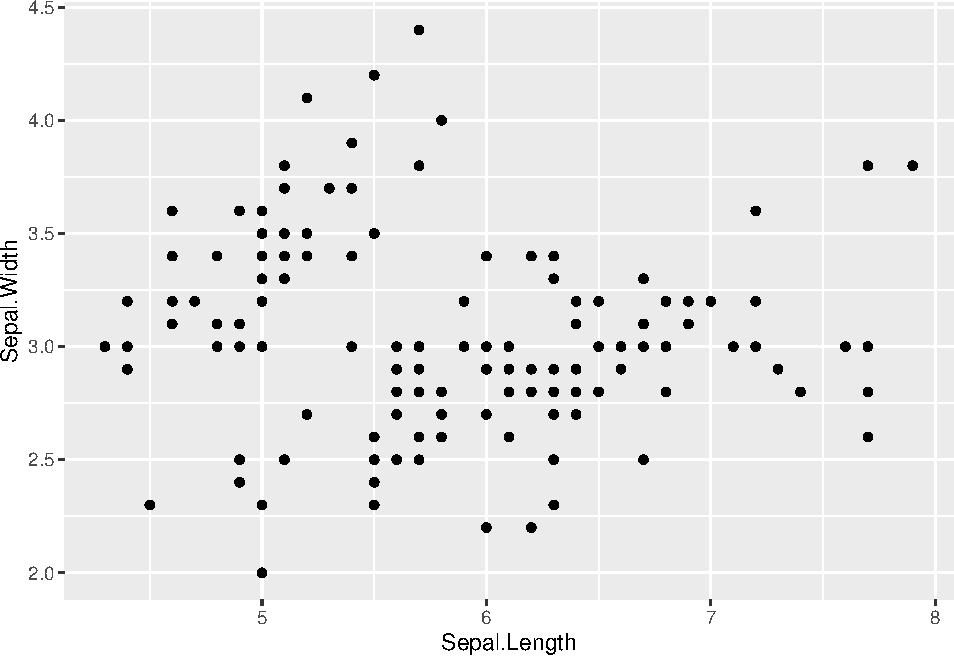
\includegraphics{41-eda_files/figure-latex/unnamed-chunk-9-1.pdf}

同じ年に、多くのデータがあるので、折れ線グラフを適切に書くことができませんでした。

\begin{Shaded}
\begin{Highlighting}[]
\NormalTok{df\_wdi\_gdppcap\_small\_short }\SpecialCharTok{\%\textgreater{}\%} \FunctionTok{filter}\NormalTok{(country }\SpecialCharTok{\%in\%} \FunctionTok{c}\NormalTok{(}\StringTok{"Japan"}\NormalTok{)) }\SpecialCharTok{\%\textgreater{}\%}
  \FunctionTok{ggplot}\NormalTok{(}\FunctionTok{aes}\NormalTok{(}\AttributeTok{x =}\NormalTok{ year, }\AttributeTok{y =}\NormalTok{ gdp\_pcap)) }\SpecialCharTok{+} \FunctionTok{geom\_line}\NormalTok{()}
\end{Highlighting}
\end{Shaded}

\includegraphics{41-eda_files/figure-latex/unnamed-chunk-10-1.pdf}

一般的には、散布図をまず、書いてみるのも一つです。

\begin{Shaded}
\begin{Highlighting}[]
\NormalTok{df\_wdi\_gdppcap\_small\_short }\SpecialCharTok{\%\textgreater{}\%}
  \FunctionTok{ggplot}\NormalTok{(}\FunctionTok{aes}\NormalTok{(}\AttributeTok{x =}\NormalTok{ year, }\AttributeTok{y =}\NormalTok{ gdp\_pcap)) }\SpecialCharTok{+} \FunctionTok{geom\_point}\NormalTok{()}
\CommentTok{\#\textgreater{} Warning: Removed 10 rows containing missing values}
\CommentTok{\#\textgreater{} (\textasciigrave{}geom\_point()\textasciigrave{}).}
\end{Highlighting}
\end{Shaded}

\includegraphics{41-eda_files/figure-latex/unnamed-chunk-11-1.pdf}

国別に、異なる色を使うことで、折れ線グラフを書くことも可能です。

\begin{Shaded}
\begin{Highlighting}[]
\NormalTok{df\_wdi\_gdppcap\_small\_short }\SpecialCharTok{\%\textgreater{}\%} \FunctionTok{drop\_na}\NormalTok{(gdp\_pcap) }\SpecialCharTok{\%\textgreater{}\%}
  \FunctionTok{ggplot}\NormalTok{(}\FunctionTok{aes}\NormalTok{(}\AttributeTok{x =}\NormalTok{ year, }\AttributeTok{y =}\NormalTok{ gdp\_pcap, }\AttributeTok{col =}\NormalTok{ country)) }\SpecialCharTok{+} \FunctionTok{geom\_line}\NormalTok{()}
\end{Highlighting}
\end{Shaded}

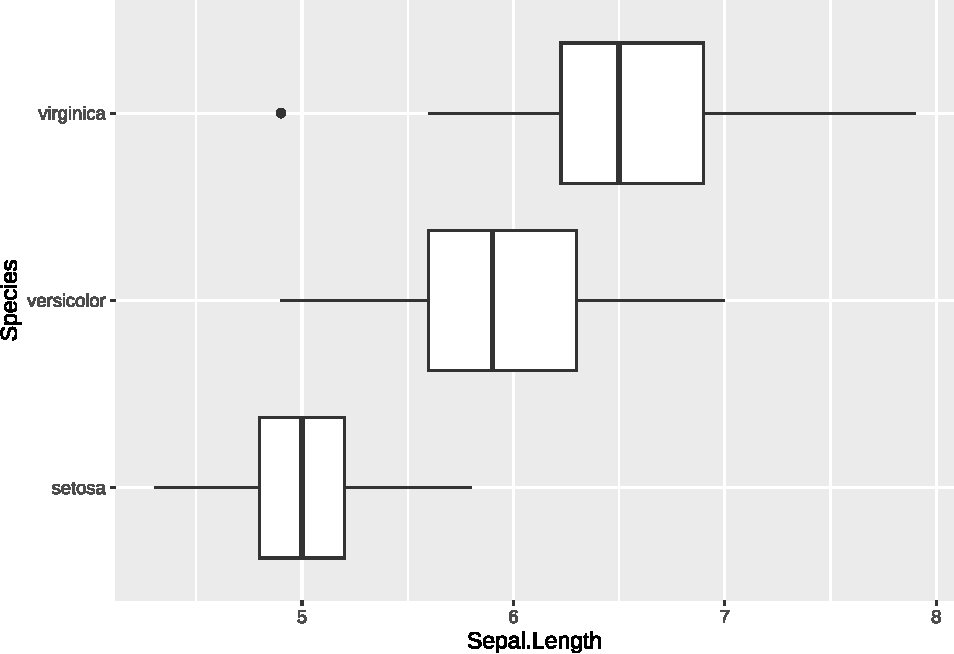
\includegraphics{41-eda_files/figure-latex/unnamed-chunk-12-1.pdf}

折線グラフと、散布図を同時に描くこともかのうです。

\begin{Shaded}
\begin{Highlighting}[]
\NormalTok{df\_wdi\_gdppcap\_small\_short }\SpecialCharTok{\%\textgreater{}\%} \FunctionTok{drop\_na}\NormalTok{(gdp\_pcap) }\SpecialCharTok{\%\textgreater{}\%}
  \FunctionTok{ggplot}\NormalTok{(}\FunctionTok{aes}\NormalTok{(}\AttributeTok{x =}\NormalTok{ year, }\AttributeTok{y =}\NormalTok{ gdp\_pcap, }\AttributeTok{col =}\NormalTok{ country)) }\SpecialCharTok{+} \FunctionTok{geom\_line}\NormalTok{() }\SpecialCharTok{+}
  \FunctionTok{geom\_point}\NormalTok{()}
\end{Highlighting}
\end{Shaded}

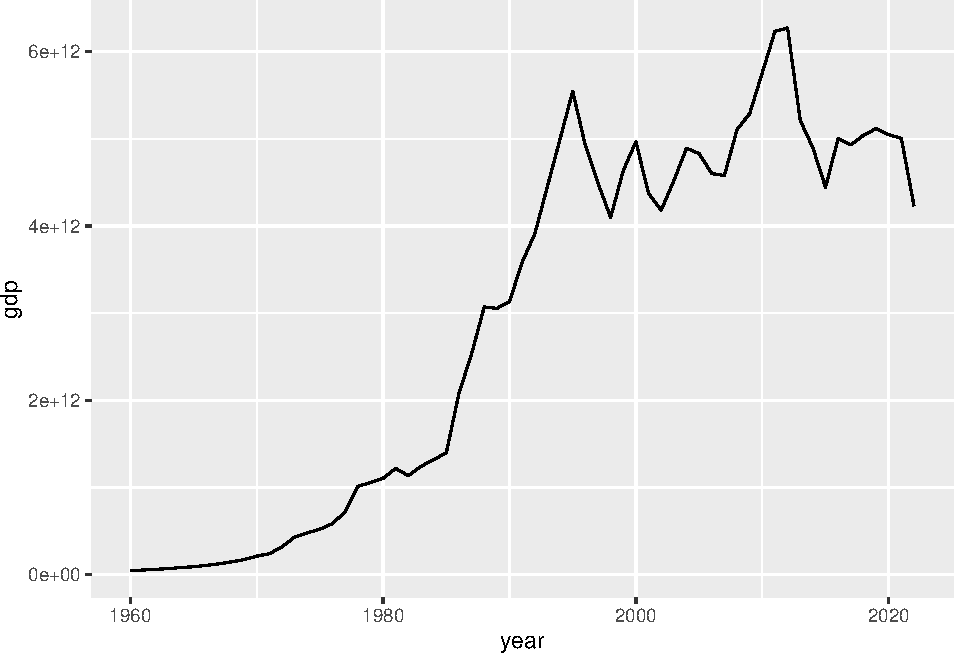
\includegraphics{41-eda_files/figure-latex/unnamed-chunk-13-1.pdf}

点を、曲線で近似する方法はいくつも知られているが、ある幅で、近似していく、LOESS が初期値となっている。\texttt{method=\textquotesingle{}loess\textquotesingle{}} を省略しても、同じ近似がなされる。\texttt{span} という値を調節することで、ことなる幅での近似曲線を書くことも可能である。初期値は、0.75。

\begin{Shaded}
\begin{Highlighting}[]
\NormalTok{df\_wdi\_gdppcap\_small\_short }\SpecialCharTok{\%\textgreater{}\%} \FunctionTok{drop\_na}\NormalTok{(gdp\_pcap) }\SpecialCharTok{\%\textgreater{}\%}
  \FunctionTok{ggplot}\NormalTok{(}\FunctionTok{aes}\NormalTok{(}\AttributeTok{x =}\NormalTok{ year, }\AttributeTok{y =}\NormalTok{ gdp\_pcap)) }\SpecialCharTok{+} 
  \FunctionTok{geom\_point}\NormalTok{(}\FunctionTok{aes}\NormalTok{(}\AttributeTok{color =}\NormalTok{ country)) }\SpecialCharTok{+} 
  \FunctionTok{geom\_smooth}\NormalTok{(}\AttributeTok{method =} \StringTok{\textquotesingle{}loess\textquotesingle{}}\NormalTok{, }\AttributeTok{formula =} \StringTok{\textquotesingle{}y \textasciitilde{} x\textquotesingle{}}\NormalTok{)}
\end{Highlighting}
\end{Shaded}

\includegraphics{41-eda_files/figure-latex/unnamed-chunk-14-1.pdf}

\hypertarget{ux30c7ux30fcux30bfux30e2ux30c7ux30eaux30f3ux30b0-data-modeling}{%
\subsection{データモデリング Data Modeling}\label{ux30c7ux30fcux30bfux30e2ux30c7ux30eaux30f3ux30b0-data-modeling}}

上の例では、曲線ではなく、直線で近似することも考えられる。

\begin{Shaded}
\begin{Highlighting}[]
\NormalTok{df\_wdi\_gdppcap\_small\_short }\SpecialCharTok{\%\textgreater{}\%} \FunctionTok{drop\_na}\NormalTok{(gdp\_pcap) }\SpecialCharTok{\%\textgreater{}\%}
  \FunctionTok{ggplot}\NormalTok{(}\FunctionTok{aes}\NormalTok{(}\AttributeTok{x =}\NormalTok{ year, }\AttributeTok{y =}\NormalTok{ gdp\_pcap)) }\SpecialCharTok{+} 
  \FunctionTok{geom\_point}\NormalTok{(}\FunctionTok{aes}\NormalTok{(}\AttributeTok{color =}\NormalTok{ country)) }\SpecialCharTok{+} 
  \FunctionTok{geom\_smooth}\NormalTok{(}\AttributeTok{method =} \StringTok{\textquotesingle{}lm\textquotesingle{}}\NormalTok{, }\AttributeTok{formula =} \StringTok{\textquotesingle{}y \textasciitilde{} x\textquotesingle{}}\NormalTok{)}
\end{Highlighting}
\end{Shaded}

\includegraphics{41-eda_files/figure-latex/unnamed-chunk-15-1.pdf}

簡単な線形回帰モデルでの、回帰直線の y-切片や、傾きは、次のコードで与えられ、p-value や、R squared の値も求められる。

この例では、年とともに、増加の傾向があること。そして、線形モデルが\$\$、90\% 程度説明していると表現される。すなわち、

は、良い、近似であることがわかる。

\begin{Shaded}
\begin{Highlighting}[]
\NormalTok{df\_wdi\_gdppcap\_small\_short }\SpecialCharTok{\%\textgreater{}\%} \FunctionTok{lm}\NormalTok{(gdp\_pcap }\SpecialCharTok{\textasciitilde{}}\NormalTok{ year, .) }\SpecialCharTok{\%\textgreater{}\%} \FunctionTok{summary}\NormalTok{()}
\CommentTok{\#\textgreater{} }
\CommentTok{\#\textgreater{} Call:}
\CommentTok{\#\textgreater{} lm(formula = gdp\_pcap \textasciitilde{} year, data = .)}
\CommentTok{\#\textgreater{} }
\CommentTok{\#\textgreater{} Residuals:}
\CommentTok{\#\textgreater{}      Min       1Q   Median       3Q      Max }
\CommentTok{\#\textgreater{} {-}14156.8  {-}3200.5   {-}507.4   3237.7  16779.2 }
\CommentTok{\#\textgreater{} }
\CommentTok{\#\textgreater{} Coefficients:}
\CommentTok{\#\textgreater{}               Estimate Std. Error t value Pr(\textgreater{}|t|)    }
\CommentTok{\#\textgreater{} (Intercept) {-}1903497.5    48007.9  {-}39.65   \textless{}2e{-}16 ***}
\CommentTok{\#\textgreater{} year             968.3       24.1   40.18   \textless{}2e{-}16 ***}
\CommentTok{\#\textgreater{} {-}{-}{-}}
\CommentTok{\#\textgreater{} Signif. codes:  }
\CommentTok{\#\textgreater{} 0 \textquotesingle{}***\textquotesingle{} 0.001 \textquotesingle{}**\textquotesingle{} 0.01 \textquotesingle{}*\textquotesingle{} 0.05 \textquotesingle{}.\textquotesingle{} 0.1 \textquotesingle{} \textquotesingle{} 1}
\CommentTok{\#\textgreater{} }
\CommentTok{\#\textgreater{} Residual standard error: 5514 on 174 degrees of freedom}
\CommentTok{\#\textgreater{}   (10 observations deleted due to missingness)}
\CommentTok{\#\textgreater{} Multiple R{-}squared:  0.9027, Adjusted R{-}squared:  0.9021 }
\CommentTok{\#\textgreater{} F{-}statistic:  1614 on 1 and 174 DF,  p{-}value: \textless{} 2.2e{-}16}
\end{Highlighting}
\end{Shaded}

\hypertarget{part-part-v-examples}{%
\part{PART V EXAMPLES}\label{part-part-v-examples}}

\hypertarget{example1}{%
\chapter{Example 1}\label{example1}}

\hypertarget{appendix-appendix}{%
\appendix}


\hypertarget{japanese}{%
\chapter{日本語の扱いについて}\label{japanese}}

\hypertarget{ux65e5ux672cux8a9eux4e2dux56fdux8a9eux97d3ux56fdux8a9e}{%
\section{日本語・中国語・韓国語}\label{ux65e5ux672cux8a9eux4e2dux56fdux8a9eux97d3ux56fdux8a9e}}

文字化けが、起こることが多く、対応が、一定せず、特に、図の表示において、Windows や、macOS や、Linux などの、OS ごとに、フォントが違ったり、それを、図のタイトルなどに、使ったりが、難しかったのですが、どうやら、現在は、どの場合も、次の設定で、解決しているようです。下の例を確認してください。特に、フォントについては、好みも関係しますから、難しいですが、ここでは、どのプラットフォーム(OS)でも、共通に扱えることを中心に書きます。

\begin{Shaded}
\begin{Highlighting}[]
\CommentTok{\# showtext を、インストールしていない場合は、一回だけ、右上の三角をクリックして実行}
\FunctionTok{install.packages}\NormalTok{(}\StringTok{\textquotesingle{}showtext\textquotesingle{}}\NormalTok{)}
\end{Highlighting}
\end{Shaded}

\hypertarget{ux30d1ux30c3ux30b1ux30fcux30b8ux3092ux30edux30fcux30c9}{%
\subsection{パッケージをロード}\label{ux30d1ux30c3ux30b1ux30fcux30b8ux3092ux30edux30fcux30c9}}

\texttt{library} によって、Package をロード(いつでも使えるように)します。

\begin{Shaded}
\begin{Highlighting}[]
\FunctionTok{library}\NormalTok{(tidyverse)}
\FunctionTok{library}\NormalTok{(showtext) }
\FunctionTok{showtext\_auto}\NormalTok{()}
\end{Highlighting}
\end{Shaded}

\hypertarget{base-r-ux3067ux30bfux30a4ux30c8ux30ebux306bux65e5ux672cux8a9e}{%
\section{Base R でタイトルに日本語}\label{base-r-ux3067ux30bfux30a4ux30c8ux30ebux306bux65e5ux672cux8a9e}}

\begin{Shaded}
\begin{Highlighting}[]
\FunctionTok{plot}\NormalTok{(cars, }\AttributeTok{main=}\StringTok{"散布図"}\NormalTok{)}
\end{Highlighting}
\end{Shaded}

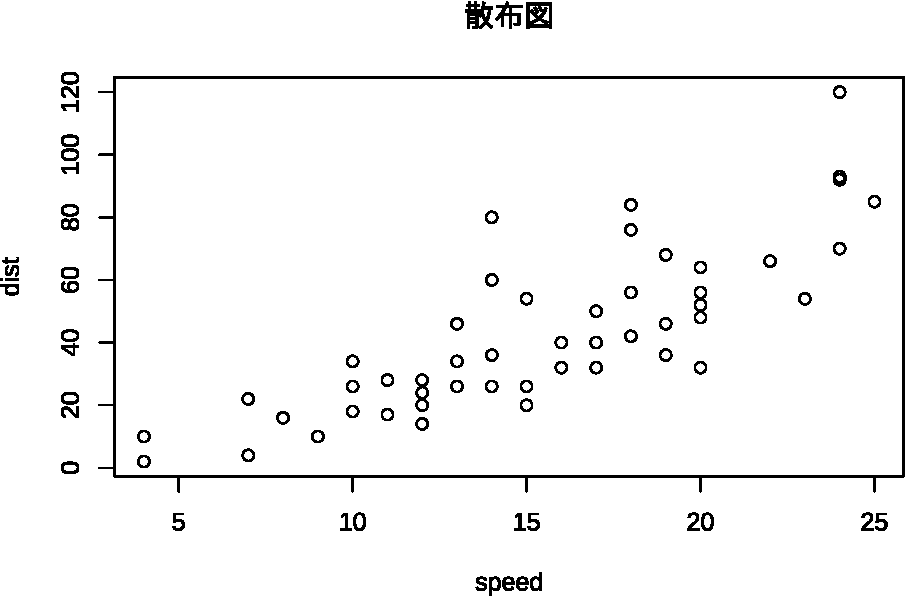
\includegraphics{81-japanese_files/figure-latex/unnamed-chunk-3-1.pdf}

\hypertarget{ux5217ux540dux3084ux30c7ux30fcux30bfux306bux65e5ux672cux8a9e}{%
\section{列名や、データに日本語}\label{ux5217ux540dux3084ux30c7ux30fcux30bfux306bux65e5ux672cux8a9e}}

\begin{Shaded}
\begin{Highlighting}[]
\NormalTok{df\_iris }\OtherTok{\textless{}{-}}\NormalTok{ iris}
\FunctionTok{colnames}\NormalTok{(df\_iris) }\OtherTok{\textless{}{-}} \FunctionTok{c}\NormalTok{(}\StringTok{"萼長"}\NormalTok{,}\StringTok{"萼幅"}\NormalTok{,}\StringTok{"葉長"}\NormalTok{,}\StringTok{"葉幅"}\NormalTok{,}\StringTok{"Species"}\NormalTok{ )}
\NormalTok{tab }\OtherTok{\textless{}{-}} \FunctionTok{data.frame}\NormalTok{(}\AttributeTok{Species =} \FunctionTok{c}\NormalTok{(}\StringTok{"setosa"}\NormalTok{, }\StringTok{"versicolor"}\NormalTok{, }\StringTok{"virginica"}\NormalTok{), }
                  \StringTok{"種別"} \OtherTok{=} \FunctionTok{c}\NormalTok{(}\StringTok{"ヒオウギアヤメ"}\NormalTok{, }\StringTok{"ブルーフラッグ"}\NormalTok{, }\StringTok{"バージニカ"}\NormalTok{))}
\NormalTok{df\_iris }\OtherTok{\textless{}{-}}\NormalTok{ df\_iris }\SpecialCharTok{\%\textgreater{}\%} \FunctionTok{left\_join}\NormalTok{(tab, }\AttributeTok{by=}\FunctionTok{c}\NormalTok{(}\StringTok{"Species"} \OtherTok{=} \StringTok{"Species"}\NormalTok{)) }\SpecialCharTok{\%\textgreater{}\%} \FunctionTok{select}\NormalTok{(}\SpecialCharTok{{-}}\DecValTok{5}\NormalTok{)}
\NormalTok{df\_iris }\SpecialCharTok{\%\textgreater{}\%} \FunctionTok{slice}\NormalTok{(}\DecValTok{1}\SpecialCharTok{:}\DecValTok{2}\NormalTok{)}
\CommentTok{\#\textgreater{}   萼長 萼幅 葉長 葉幅           種別}
\CommentTok{\#\textgreater{} 1  5.1  3.5  1.4  0.2 ヒオウギアヤメ}
\CommentTok{\#\textgreater{} 2  4.9  3.0  1.4  0.2 ヒオウギアヤメ}
\end{Highlighting}
\end{Shaded}

\hypertarget{kable-ux3067ux8868ux793a}{%
\section{\texorpdfstring{\texttt{kable} で表示}{kable で表示}}\label{kable-ux3067ux8868ux793a}}

\begin{Shaded}
\begin{Highlighting}[]
\NormalTok{knitr}\SpecialCharTok{::}\FunctionTok{kable}\NormalTok{(df\_iris[}\DecValTok{1}\SpecialCharTok{:}\DecValTok{6}\NormalTok{, ])}
\end{Highlighting}
\end{Shaded}

\begin{tabular}{r|r|r|r|l}
\hline
萼長 & 萼幅 & 葉長 & 葉幅 & 種別\\
\hline
5.1 & 3.5 & 1.4 & 0.2 & ヒオウギアヤメ\\
\hline
4.9 & 3.0 & 1.4 & 0.2 & ヒオウギアヤメ\\
\hline
4.7 & 3.2 & 1.3 & 0.2 & ヒオウギアヤメ\\
\hline
4.6 & 3.1 & 1.5 & 0.2 & ヒオウギアヤメ\\
\hline
5.0 & 3.6 & 1.4 & 0.2 & ヒオウギアヤメ\\
\hline
5.4 & 3.9 & 1.7 & 0.4 & ヒオウギアヤメ\\
\hline
\end{tabular}

\hypertarget{ggplot-ux3067ux30b0ux30e9ux30d5ux3092ux4f5cux6210}{%
\section{\texorpdfstring{\texttt{ggplot} でグラフを作成}{ggplot でグラフを作成}}\label{ggplot-ux3067ux30b0ux30e9ux30d5ux3092ux4f5cux6210}}

\begin{Shaded}
\begin{Highlighting}[]
\FunctionTok{ggplot}\NormalTok{(df\_iris, }\FunctionTok{aes}\NormalTok{(}\AttributeTok{x =} \StringTok{\textasciigrave{}}\AttributeTok{葉長}\StringTok{\textasciigrave{}}\NormalTok{, }\AttributeTok{y =} \StringTok{\textasciigrave{}}\AttributeTok{葉幅}\StringTok{\textasciigrave{}}\NormalTok{, }\AttributeTok{col =} \StringTok{\textasciigrave{}}\AttributeTok{種別}\StringTok{\textasciigrave{}}\NormalTok{)) }\SpecialCharTok{+}
  \FunctionTok{geom\_point}\NormalTok{() }\SpecialCharTok{+} \FunctionTok{labs}\NormalTok{(}\AttributeTok{title =} \StringTok{"散布図"}\NormalTok{, }\AttributeTok{x =} \StringTok{"葉長"}\NormalTok{, }\AttributeTok{y =} \StringTok{"葉幅"}\NormalTok{)}
\end{Highlighting}
\end{Shaded}

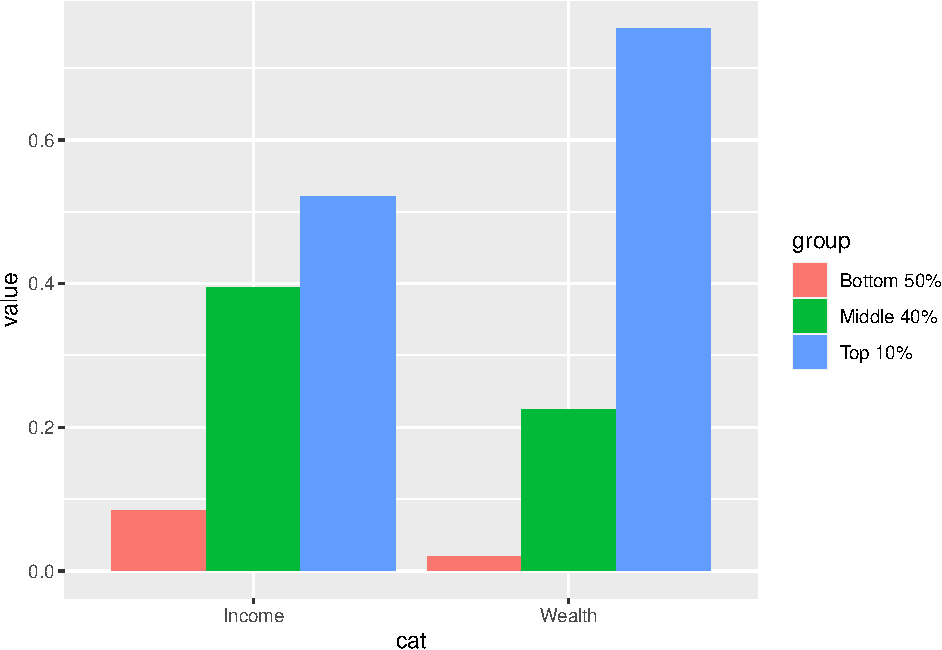
\includegraphics{81-japanese_files/figure-latex/unnamed-chunk-5-1.pdf}

\hypertarget{ux5099ux8003-1}{%
\section{備考:}\label{ux5099ux8003-1}}

実は、一番難しいのが、PDF の作成だと思いますが、一応、上のものも、PDF を作成することが可能です。 下のリンクのファイルを、いろいろな、形式で、出力してみてください。R Notebook と、PDF に出力したもののリンクを付けておきます。

\begin{itemize}
\tightlist
\item
  \href{https://ds-sl.github.io/intro2r/Rmarkdown-J.nb.html}{R Notebook}

  \begin{itemize}
  \tightlist
  \item
    右上の Code ボタンから、Rmd ファイルも取得できます。
  \end{itemize}
\item
  \href{https://ds-sl.github.io/intro2r/Rmarkdown-J.html}{R Notebook RMD}

  \begin{itemize}
  \tightlist
  \item
    Rmd の中身がテキストで表示されますから、コピーして、新規作成した、RNotebook ファイルに貼り付けることも可能です。
  \end{itemize}
\item
  \href{https://ds-sl.github.io/intro2r/Rmarkdown-J.pdf}{PDF}

  \begin{itemize}
  \tightlist
  \item
    通常のPDFも、やはり PDF 形式の、beamer presentation も作成できます。
  \end{itemize}
\end{itemize}

詳細は、これらのファイルに記載されていますから、参考にしてください。

\hypertarget{ux53c2ux8003ux65e5ux672cux8a9eux306eux8868ux793aux306bux3064ux3044ux3066}{%
\section{参考:日本語の表示について}\label{ux53c2ux8003ux65e5ux672cux8a9eux306eux8868ux793aux306bux3064ux3044ux3066}}

\begin{quote}
日本語が適切に表示されない!?
\end{quote}

簡単ではなく、未解決の部分が何かなどを含め、わたしも十分理解できているか不明であるが、理解できていると思われる範囲で、備忘録のように記します。

R を使うという場合に限っても、R Studio IDE を使う場合、RStudio Cloud を使う場合、Google colab を使う場合、他のプラットフォームで使う場合で違ってくると思われますが、上にあげた、三種類のプラットフォームで確かめられるものについて書いていく。上に書いた以外に、R Studio IDE を、Windows 上で使う場合と、Mac 上で使う場合(Mac のシステムは Unix 系であるが、さまざまな Linux )でも、状況が異なるかもしれません。そこで、場合分けをして書いていくほうが安全ですが、それは、極力避け、どれにでも適用可能な方法を模索しながら書いていこうと思います。個人的に、日常的に分断を避ける努力をすることが大切だと思っていることも背景にある。さらに、ソフトウェア開発者は、むろん、そのような差異を理解して、どの環境でも、可能なように設計することを心がけていると思われますし、そのようなものが、R Project の正規のパッケージとして採用されていくべきだとも考えていますので、多少、理想も入っているが、これを基本として書いていこうと思います。十分なチェックができていないものもあるので、不具合などは、ぜひ、お知らせ願いたい。この文章も少しずつ、改善していければと思う。

通常、日本語、中国語、韓国語などが適切に表示できない場合は、文字のエンコーディング(Encoding: どのような情報として記録されているか)と、フォントの問題、さらに、システムがこれらをどう処理しているかの問題があると思われます。しかし、R の利用者として考えると、文字化けが起きたり、適切に文字が表示されないのは、以下の三つに分けられるようです。

\begin{enumerate}
\def\labelenumi{\arabic{enumi}.}
\tightlist
\item
  データファイルなどを読み込んだときに適切に表示されない
\item
  図の中のタイトルなどが、適切に表示されない
\item
  R Markdown の出力において、適切に表示されない
\end{enumerate}

\hypertarget{ux30c7ux30fcux30bfux30d5ux30a1ux30a4ux30ebux306eux8aadux307fux8fbcux307f}{%
\subsection{データファイルの読み込み}\label{ux30c7ux30fcux30bfux30d5ux30a1ux30a4ux30ebux306eux8aadux307fux8fbcux307f}}

\begin{itemize}
\tightlist
\item
  tidyverse に含まれる readr には、guess\_encoding が含まれており、一般的には、たとえば、

  \begin{itemize}
  \tightlist
  \item
    read\_csv(``./data/file\_name.csv'') とすると、一番可能性の高いエンコーディングで読み込まれるようになっています。
  \end{itemize}
\item
  使い方:guess\_encoding(file, n\_max = 10000, threshold = 0.2) とあり、10000行で推測されたエンコーディング、または、確率を計算することを 初期設定値(Default)にしてます。Help によると、すべての行をチェックする場合は、n\_max = -1 とすることが書かれています。
\item
  これで問題がない場合が多いです。他の、readr 関数も同様です。しかし、これは、あくまでも、CSV などのテキストファイルについてです。
\item
  なお、read\_csv などにも、guess\_max = min(1000, n\_max) もありますが、これは、column type を決めるためのものである。
\item
  read.csv() など、base R では、fileEncoding = ````, encoding =''unknown'' がオプションに含まれていたので、指定して読み込むことが通常でした。
\end{itemize}

\hypertarget{ux56f3ux306eux4e2dux306eux30c6ux30adux30b9ux30c8}{%
\subsection{図の中のテキスト}\label{ux56f3ux306eux4e2dux306eux30c6ux30adux30b9ux30c8}}

\begin{itemize}
\tightlist
\item
  基本的には、日本語を表示できるフォントがインストールされていて、図の表示の前にlibrary(showtext); showtext\_auto() となっていれば、これ以降の図は、問題なく、表示されるはずです。
\item
  通常使っている、コンピュータ以外で、使うときに、フォントが入っていない場合などは、\texttt{tinytex} の命令を使って、\texttt{tinytex::tlmgr\_install("ipaex")} とすれば、PDF を作成するときも、IPA フォント(International Phonetic Alphabet)を使えます。
\item
  二種類以上のフォントを使い分けたいときは、名前をつけて、それを family = name で指定する。

  \begin{itemize}
  \tightlist
  \item
    showtext: Using Fonts More Easily in R Graphs 参照。
  \end{itemize}
\end{itemize}

\hypertarget{r-markdown-ux306eux51faux529b}{%
\subsection{R Markdown の出力}\label{r-markdown-ux306eux51faux529b}}

\begin{itemize}
\tightlist
\item
  PDF 作成には、\TeX システムを使っているので、日本語を扱えるように、tex-engine や、document class や、mainfont を設定する必要があるが、R Markdown ファイルの YAML に、以下を加えれば問題がないようである。
\end{itemize}

\begin{verbatim}
header-includes:
  - \usepackage{xeCJK}
  - \setCJKmainfont{ipaexm.ttf}
  - \setCJKsansfont{ipaexg.ttf}
  - \setCJKmonofont{ipaexg.ttf}
\end{verbatim}

\hypertarget{bookdown}{%
\subsection{\texorpdfstring{\texttt{bookdown}}{bookdown}}\label{bookdown}}

\texttt{bookdown} を使って、電子書籍を出版する場合には、\href{https://bookdown.org/yihui/bookdown/}{\texttt{bookdown} (リンク)} を参照してください。

日本語におけるテンプレートは、\href{https://github.com/icu-hsuzuki/bs4_book_template}{こちら} にあります。まずは、ページの下にある、README を読んでください。

\hypertarget{ux53c2ux8003ux3068ux3057ux305fux3082ux306e}{%
\subsection{参考としたもの}\label{ux53c2ux8003ux3068ux3057ux305fux3082ux306e}}

\hypertarget{showtext-using-fonts-more-easily-in-r-graphs}{%
\subsubsection{showtext: Using Fonts More Easily in R Graphs}\label{showtext-using-fonts-more-easily-in-r-graphs}}

\begin{itemize}
\tightlist
\item
  \url{https://CRAN.R-project.org/package=showtext}

  \begin{itemize}
  \tightlist
  \item
    \url{https://cran.r-project.org/web/packages/showtext/readme/README.html}
  \item
    showtext: Using Fonts More Easily in R Graphs:

    \begin{itemize}
    \tightlist
    \item
      \url{https://cran.r-project.org/web/packages/showtext/vignettes/introduction.html}
    \item
      \url{https://fonts.google.com}
    \end{itemize}
  \end{itemize}
\end{itemize}

\hypertarget{sysfonts-loading-fonts-into-r}{%
\subsubsection{sysfonts: Loading Fonts into R}\label{sysfonts-loading-fonts-into-r}}

\begin{itemize}
\tightlist
\item
  \url{https://CRAN.R-project.org/package=sysfonts}

  \begin{itemize}
  \tightlist
  \item
    \url{https://cran.r-project.org/web/packages/sysfonts/sysfonts.pdf}
  \end{itemize}
\end{itemize}

\hypertarget{foods4all-examples-of-graphs}{%
\subsubsection{foods4all: Examples of Graphs}\label{foods4all-examples-of-graphs}}

\begin{itemize}
\tightlist
\item
  \url{https://foods4all.github.io/examples/examples_of_graphs.html}

  \begin{itemize}
  \tightlist
  \item
    77.2 Japanese Environments 日本語環境(昔の記事:Last Updated: 2020-04-22)
  \end{itemize}
\end{itemize}

\hypertarget{tools}{%
\chapter{IT ツール}\label{tools}}

\begin{quote}
いくつかの便利なツールについて紹介します。
\end{quote}

\hypertarget{git-ux3068-github}{%
\section{Git と GitHub}\label{git-ux3068-github}}

Git は バージョン管理システムで、GitHub はそれを、活用し、かつ他のメンバーと協力して開発など、さまざまな活動をするためのサイトです。公開が基本となっています。非公開にすることも可能ですが、公開することで、世界中のひとたちと協力していくことが可能になりますので、その利点も学んでいただければと思います。

\hypertarget{ux6982ux8981}{%
\subsection{概要}\label{ux6982ux8981}}

RStudio で R を使っている場合、Git-GitHub-RStudio の連携で使うことをお勧めします。しかし、これらは、三つとも、まったく異なるものですから、簡単な概要を書いておくことにします。

\hypertarget{git}{%
\subsubsection{Git}\label{git}}

これは、ファイルのバージョン(更新履歴)の管理システムで、単独で機能します。他の、プログラムなどに関係しない、他の文書ファイルであっても、バージョンを管理する場合に活用できます。特に、テキスト・ファイルの場合には、どこがどう改訂されているかを確認することもできます。また、基本的には、Unix の Shell プログラムで動作させるのが一般的です。Mac は、Unix システムの上に構築されているため、最初から、ユーティリティ(Utility)\textgreater{} ターミナル(Terminal)で、Shell コマンドが利用可能になっていますが、Windows の場合には、bash と呼ばれる Shell プログラムをインストールすることをお勧めします。Windows システムについてよくご存知の方は、他の方法を使っていただいて構いませんが、Git のインストールの時に、Git bash を選択して、簡単に インストールできますし、Unix システムの基本を理解するチャンスでもあり、Mac とも同じ環境で説明できますから、ここでは、そちらを使います。Shell コマンドは、R Studio の中のターミナルを使って、利用することも可能です。(注:Windows のコマンド・プロンプト、または、パワー・シェルをお使いの方は、利用環境が変化する可能性がありますから、そのまま使われる方が良いかもしれません。)

基本的なコマンドとしては、以下のものがあります。いまは、このようなものがある程度に、眺めておいてください。

\begin{itemize}
\tightlist
\item
  \texttt{git\ init}: 特定のディレクトリ(フォルダ)で バージョン管理を始める時に使います。
\item
  \texttt{git\ status}: 現在の状況を確認するときに使います。
\item
  \texttt{git\ diff\ file\_name}: ファイルへの変更を確認します。
\item
  \texttt{git\ log}: 過去の commit による履歴を確認する時に使います。
\item
  \texttt{git\ add\ file\_name}: ステージングという中間的な場所に登録します。
\item
  \texttt{git\ commit\ -m\ "log\ message\ here"}: ステージングにあるものを、確定させます。引用符で囲まれた短いコメントを加えます。50文字が上限です。
\item
  \texttt{git\ help}: Help のリストが表示されます。

  \begin{itemize}
  \tightlist
  \item
    例:\texttt{git\ help\ init} などと入力すると、説明を見ることができます。
  \end{itemize}
\end{itemize}

\hypertarget{git-hub}{%
\subsubsection{Git Hub}\label{git-hub}}

Git でバージョン管理されているディレクトリ(フォルダ)の状態を示す、クラウドサービスです。更新されている、状態を確認するとともに、変更履歴なども確認できます。また、Git Hub サービスを利用して、ファイルを公開、共有することも可能です。Pages サイトを利用することで、ホームページとして HTML ファイルなどを公開することもできるため、レポートを公開したり、この電子書籍のように、\texttt{bookdown} パッケージを利用して作成したものを、インターネット上に公開することも可能です。

お気付きかと思いますが、この電子書籍も、リンクされている、他の文書も、URL(アドレス)をみると、GitHub になっていますし、パッケージや、データなども、GitHub へのリンクが示されている割合が、非常に高いと思います。

最初に、Git で管理されている、ディレクトリ(フォルダ)(これを、ローカル・リポジトリと言います)と、GitHub 内のリポジトリ(リモート・リポジトリまはたアップストリーム・リポジトリと言います。ここでは、リモート・リポジトリと呼ぶことにします)を結びつけるステップが必要です。

\hypertarget{rstudio-ux9023ux643a}{%
\subsubsection{RStudio 連携}\label{rstudio-ux9023ux643a}}

コマンドライン(シェル)で行う作業や、ローカル・リポジトリを、リモート・リポジトリに結びつける作業を、RStudio の中で行うことが可能です。

\hypertarget{ux306fux3058ux3081ux304bux305f}{%
\subsection{はじめかた}\label{ux306fux3058ux3081ux304bux305f}}

\begin{enumerate}
\def\labelenumi{\arabic{enumi}.}
\tightlist
\item
  Git のインストール
\end{enumerate}

\begin{itemize}
\tightlist
\item
  Windows と Mac で異なりますので注意が必要です。Mac については、\textbf{Mac} と書いてあるところを読んでください。
\item
  \textbf{Windows} の場合は、\href{https://git-scm.com/download/win}{git-scm} にアクセスしてダウンロード、インストールしてください。セットアップ(Setup)で、2箇所、注意点があります、それ以外は、すべて、初期設定のままで変更は必要ありません。

  \begin{itemize}
  \tightlist
  \item
    Choosing the default editor used by Git: 設定で、エディタ(Editor)を設定しますが、vi, vim に慣れていない方は、nano を選択することをお勧めします。(nano\footnote{GNU nanoは、コンソールウィンドウで動作する小型でフレンドリーなテキストエディタです。(GNU nano is a small and friendly text editor running in the console window.)} は、メニューが下に出るので、それを見て操作することが可能なエディターです。)
  \item
    Adjusting Your Path Environment: Windows の コマンドライン・ツール(command line prompt) を使っていない方は、Git Bash のインストールを選択してください。さらに、Git and optional Unix tools from the Windows Command Prompt を選択することをお勧めしますが、上で書いたように、Windows の コマンド・プロンプトになれておられる方で、それを使い続けたいかたは、Use Git from Git Bash only を選択されるのが良いかもしれません。
  \item
    最後に、RStudio の設定(Tools \textgreater{} Global Option)で、Terminal から、Git Bash を選択\footnote{自動的に選択されているかもしれません}し、Tools から、New Terminal を選択\footnote{すでにタブがあればこの作業は不要です}します。
  \end{itemize}
\item
  \textbf{Mac} は、最初から、Install されていると思います。ユーティリティ(Utility)\textgreater{} ターミナル(Terminal)を開いて\footnote{RStudio を既にお使いの方は、左下の窓枠から、Terminal タブを選択できますので、それを使うことも可能です。}、\texttt{git\ -\/-version} とすると、インストールされているバージョンが表示されると思います。バージョンがでない場合には、Install するかと聞かれます。このときに、Git だけをインストールすることも、Xcode という開発環境を同時にインストールすることも可能です。(インストールするように指示が出なければ、App Store からも、インストールできます。もし、そのあとで、git などのコマンドで xcrun: error などとエラーが出たら、\texttt{xcode-select\ -\/-install} としてください。)インストールが終了したら、もう一度、\texttt{git\ -\/-version} と Terminal に入力して、結果を確認してください。
\end{itemize}

\begin{enumerate}
\def\labelenumi{\arabic{enumi}.}
\setcounter{enumi}{1}
\tightlist
\item
  GitHub のアカウント取得
\end{enumerate}

\begin{itemize}
\tightlist
\item
  \href{https://github.com}{GitHub サイト} に、アカウントを作成します。アカウント名は、短く、分かりやすく、覚えやすいものをよく考えて決めてください。Email Address だけで、無償で作成できます。
\end{itemize}

\begin{enumerate}
\def\labelenumi{\arabic{enumi}.}
\setcounter{enumi}{2}
\tightlist
\item
  RStudio の 左下の窓枠のTerminal タブ\footnote{Terminal がない場合は、Tools \textgreater{} Terminal \textgreater{} New Terminal とすると表示されます。}から、GitHub アカウントに連携する設定を行います。 下の2行を、1行ずつ、コピーして、Terminal に入力してください。
\end{enumerate}

\begin{verbatim}
git config --global user.name "Your Name" # GitHub の User Name
git config --global user.email "your@email.com" # GitHub に登録したメールアドレス
\end{verbatim}

\begin{enumerate}
\def\labelenumi{\arabic{enumi}.}
\setcounter{enumi}{3}
\tightlist
\item
  RStudio の、Tools \textgreater{} Global Opton の、Git/SVN タブを開き、Git Executable とあるところに、Git 実行プログラムのある場所を入れます。
\end{enumerate}

\begin{itemize}
\tightlist
\item
  \textbf{Windows} の場合は、\texttt{C:/Program\ Files/Git/bin/git.exe} だと思いますが、Browse ボタンから確認してください。
\item
  \textbf{Mac} の場合は、\texttt{/usr/bin/git} になるかと思いますが、Browse ボタンから確認してください。
\end{itemize}

\begin{enumerate}
\def\labelenumi{\arabic{enumi}.}
\setcounter{enumi}{4}
\item
  その下に、Create RSA key とありますから、それを押し、Create ボタンを押しててください\footnote{Passphrase (optional) と出ますが、無視してくださって構いません。}。すると、View RSA key から、暗号キーも確認できます。(この作業は、Terminal から、\texttt{ssh-keygen\ -t\ rsa} として作成することも可能です。この作業で、\texttt{\textasciitilde{}/.ssh/} 内に、SSH キーが記述されたファイルが作成されます。)
\item
  GitHub アカウントで公開鍵を利用できるようにします。まず、RStudio の方で作成した、RSA key (Tools の、Global Option の Git/SVN)の下にある view を押すと見ることができ、上に、書いてあるように、そこに出てきたものを、コピーします。次に、GitHubにログインし、右上のアイコンの右の三角から、設定(Setting)を選択し、SSH公開鍵(SSH and GPG Keys)を選択します。新しい公開鍵を追加(New SSH Key)を選択すると、SSH キーを貼り付けることができます。(リポジトリの左上にある、アカウント名をクリックし現れるダッシュボードの左上の大きなアイコンをクリックしても「アカウント設定」が現れ、SSH and GPG Keysを見つけることができると思います。)
\end{enumerate}

(なお、RStudio ではなく、Terminal からコピーするときは、Unix では、\texttt{pbcopy\ \textless{}\ \textasciitilde{}/.ssh/id\_rsa.pub} などとします。Windows の場合は、\texttt{pbcopy} が使えない可能性があるので、そのときは、Terminal から、Git Bash を使い、\texttt{use\ \textless{}\ \textasciitilde{}/.ssh/id\_rsa.pub} とします。Terminal に慣れておられない方には、上に紹介した、RStudio からコピーする方が簡便かと思います。)

\begin{enumerate}
\def\labelenumi{\arabic{enumi}.}
\setcounter{enumi}{6}
\tightlist
\item
  これで設定終了ですので、R Studio を再起動させてください。
\end{enumerate}

\hypertarget{github-ux306bux3042ux308bux30eaux30e2ux30fcux30c8ux30eaux30ddux30b8ux30c8ux30earemote-repoux304bux3089ux59cbux3081ux308bux5834ux5408}{%
\subsection{GitHub にあるリモート・リポジトリ(Remote Repo)から始める場合}\label{github-ux306bux3042ux308bux30eaux30e2ux30fcux30c8ux30eaux30ddux30b8ux30c8ux30earemote-repoux304bux3089ux59cbux3081ux308bux5834ux5408}}

\begin{enumerate}
\def\labelenumi{\arabic{enumi}.}
\tightlist
\item
  GitHub にログインして、既存のリポジトリを開きます。
\item
  Code の、Clone から、リンク先のアドレスを入手。https と SSH を選べますが、SSH を選び、コピーします。
\item
  RStudio から、New Project とし、Version Control を選択し、ディレクトリーを決めたら、上でコピーした、ものを、貼り付けて、Project を作成します。
\end{enumerate}

この手続きで、リモート・リポジトリのファイルがすべて、RStudio のプロジェクトに入ります。

実はこの手続きで、公開されている、他のリポジトリも取り込むことができます。ただし、編集して、改訂していくには、自分のリポジトリに、繋ぐことになります。そのときは、次の項目を見てください。

\hypertarget{ux81eaux5206ux306eux30b3ux30f3ux30d4ux30e5ux30fcux30bfux306eux30eaux30ddux30b8ux30c8ux30ealocal-repoux304bux3089ux59cbux3081ux308bux5834ux5408}{%
\subsection{自分のコンピュータのリポジトリ(Local Repo)から始める場合}\label{ux81eaux5206ux306eux30b3ux30f3ux30d4ux30e5ux30fcux30bfux306eux30eaux30ddux30b8ux30c8ux30ealocal-repoux304bux3089ux59cbux3081ux308bux5834ux5408}}

\begin{enumerate}
\def\labelenumi{\arabic{enumi}.}
\tightlist
\item
  RStudio から新しい、プロジェクト(Project) を作成 \texttt{test0} としておきましょう。
\item
  GitHub に、新しい、レポジトリを作成して繋げる
\end{enumerate}

\begin{itemize}
\tightlist
\item
  自分の GitHub アカウントに、新しい、レポジトリをプロジェクトと同じ名前 \texttt{test0} で作成します。同じ名前でなくてもかまわないのですが、関連がしやすいので、同じ名前がお勧めです。
\item
  Quick Setup というページが表示されますから、その、下の Set up in Desktop or の右から、https と SSH を選べますが、SSH を選び、コピーします。
\item
  プロジェクトの中の 左下の窓枠の、Terminal から次を実行します。
\end{itemize}

\begin{verbatim}
echo "# Project test0" >> README.md # REAME の表題を書きます。
git init
git add README.md
git commit -m "First commit. README.md"
git branch -M main
git remote add origin `git@github.com:icu-hsuzuki/test0.git`
# わたしのアカウントの場合には、コピーしたものを貼り付けると、上のようになります。
git push -u origin main
\end{verbatim}

再起動すると、プロジェクトの右上の窓枠に、Git と表示されていると思います。開いて、いくつかファイル名があれば、これを選択し、Commit ボタンを押し、短い message を書いて、Commit とし、そのあとで、Push ボタンを押してください。 \texttt{HEAD\ -\textgreater{}\ main} と表示されれば、OK です。

\hypertarget{github-pages-ux306bux3064ux3044ux3066}{%
\subsection{GitHub Pages について}\label{github-pages-ux306bux3064ux3044ux3066}}

GitHub は、Web 上のサービスですが、たとえ、リポジトリーの中に、HTML ファイルなどが存在しても、ブラウザーで表示させることはできません。公開する方法として、わたしは、以下のようにしています。

公開しブラウザーで読めるようにしたいファイルを、\texttt{docs} という ディレクトリに入れます。Setting を選択し、左の帯から、Pages を選び、Branch を、\texttt{main}、\texttt{/docs} として、Save します。すると、docs に入っているファイルは、リンクを指定すれば、ブラウザーで、見ることができます。

リンクは、まず、リポジトリーの右上の、About の右のギアマークから、Use your GitHub Pages website に、チェックを入れると、URL が表示されますから、その URL に続けて、ファイル名を加えたものが、そのファイルの、リンクとなります。

\hypertarget{bookdown-ux30d1ux30c3ux30b1ux30fcux30b8ux306bux3088ux308bux96fbux5b50ux66f8ux7c4dux306eux57f7ux7b46}{%
\subsection{Bookdown パッケージによる、電子書籍の執筆}\label{bookdown-ux30d1ux30c3ux30b1ux30fcux30b8ux306bux3088ux308bux96fbux5b50ux66f8ux7c4dux306eux57f7ux7b46}}

\href{https://github.com/rstudio/bookdown}{bookdown} を利用して、始める方法を簡単に記します。

Git-GitHub-RStuio の設定は済んでいると仮定して書きます。また、Bookdown を利用するには、\texttt{bookdown} パッケージのインストールが必要です。RStudio の Tools から、Install Packages を選択して、インストールしてください。また、\texttt{bs4\_book} スタイルを利用する場合は、RStudio などのバージョンによっては、\texttt{bslib} と \texttt{downlit} も、インストールする必要があるようです。

以下では、R Studio で新しい、プロジェクトとして始める場合と、テンプレート・リポジトリ を使う方法を説明します。

\hypertarget{rstudio-ux3067ux306eux8a2dux5b9a}{%
\subsubsection{RStudio での設定}\label{rstudio-ux3067ux306eux8a2dux5b9a}}

\begin{enumerate}
\def\labelenumi{\arabic{enumi}.}
\tightlist
\item
  新しい book プロジェクトを始めます、標準設定の \texttt{book} と、\texttt{bs4\_book} を選択できます。このディレクトリ(フォルダ。ローカル・リポジトリと呼びます)の名前をリモート・リポジトリの名前と同じにして、作成します\footnote{異なる名前でも可能ですが、特別な理由がない限り同じにしておいた方が良いでしょう}。
\item
  Files の、Rename 機能を使って \texttt{\_book} ディレクトリ(フォルダ)の名前を、\texttt{docs} に変更します。
\item
  \texttt{\_bookdown.yml} を編集し次の行を加えます(私は2行目に入れています)。\\
  \texttt{output\_dir:\ docs}\strut \\
  GitHub Pages の機能を使って、公開するための変更です。
\item
  \textbf{@GitHub:} 新いリポジトリー(リモート・リポジトリと言います)を作成します。ローカル・リポジトリと同じ名前にし、簡単な説明を加えます。
\item
  左下の窓枠から、Terminal タブを選択します。 以下は例です。\texttt{git\ remote\ add\ origin} のところは、適当に変更してください。
\end{enumerate}

\begin{verbatim}
echo "# ds-book" >> README.md
git init
git add README.md
git commit -m "first commit"
git branch -M main
git remote add origin git@github.com:icu-hsuzuki/ds4aj.git # 変更
git push -u origin main
\end{verbatim}

\begin{enumerate}
\def\labelenumi{\arabic{enumi}.}
\setcounter{enumi}{4}
\tightlist
\item
  RStudio を一旦終了し、もう一度、そのプロジェクトを立ち上げると、右上の窓枠に、Git タブが表示されるはずです。
\item
  Build から、Build Book ボタンを利用すれば、作成されます。
\item
  Git タブから: Commit ``first build'' とし、 Push をします。
\item
  \textbf{@GitHub:} Settings から、Pages \textgreater{} main \textgreater{} docs と変更すると、公開されます。
\item
  Code に戻り、About の右のギアマークから、
\end{enumerate}

\hypertarget{ux4ed6ux306e-pc-ux3067ux306eux4f5cux696d}{%
\paragraph{他の PC での作業}\label{ux4ed6ux306e-pc-ux3067ux306eux4f5cux696d}}

\begin{enumerate}
\def\labelenumi{\arabic{enumi}.}
\tightlist
\item
  Login to GitHub account
\item
  Copy SSH address under Code\textgreater Clone
\item
  Create a new project using Version Control:Git with the SSH address by setting the directory name
\item
  Edit README.md and test Git Commit and Push
\end{enumerate}

\hypertarget{ux30c6ux30f3ux30d7ux30ecux30fcux30c8ux3092ux5229ux7528ux3059ux308bux65b9ux6cd5}{%
\subsubsection{テンプレートを利用する方法}\label{ux30c6ux30f3ux30d7ux30ecux30fcux30c8ux3092ux5229ux7528ux3059ux308bux65b9ux6cd5}}

\hypertarget{bookdown-demo}{%
\paragraph{bookdown-demo}\label{bookdown-demo}}

\href{https://bookdown.org/yihui/bookdown/}{\texttt{bookdown} の電子書籍(bookdown: Authoring Books and Technical Documents with R Markdown)} の、はじめてみよう(Get started)から、GitHub リポジトリー \href{https://github.com/rstudio/bookdown-demo}{rstudio/bookdown-demo} にリンクがついています。

\begin{enumerate}
\def\labelenumi{\arabic{enumi}.}
\tightlist
\item
  自分の、GitHub アカウントに、ログインします。
\item
  \href{https://github.com/rstudio/bookdown-demo}{rstudio/bookdown-demo} にアクセスし、Use this template から、create a new repository を選択します。
\item
  自分のアカウントの中に、コピーされたリポジトリーがつくられます。
\item
  上で説明した「GitHub にあるリモート・リポジトリ(Remote Repo)から始める場合」を利用してください。
\end{enumerate}

よくできているテンプレートです。しかし、このままでは、公開されません。\href{https://bookdown.org/yihui/bookdown/}{bookdown: Authoring Books and Technical Documents with R Markdown} には、いくつかの公開方法が書かれていますから、参照してください。

\hypertarget{jtr13bookdown-template}{%
\paragraph{\texorpdfstring{\texttt{jtr13/bookdown-template}}{jtr13/bookdown-template}}\label{jtr13bookdown-template}}

YouTube ビデオ \href{https://www.youtube.com/watch?v=m5D-yoH416Y}{5分間で、bookdown の本を作成する方法(How to create a bookdown book in 5 minutes)} で紹介されているものです。

\begin{enumerate}
\def\labelenumi{\arabic{enumi}.}
\tightlist
\item
  自分の、GitHub アカウントに、ログインします。
\item
  \href{https://github.com/jtr13/bookdown-template}{jtr13/bookdown-template} にアクセスし、Use this template から、create a new repository を選択します。
\item
  自分のアカウントの中に、コピーされたリポジトリーがつくられます。
\item
  上で説明した「GitHub にあるリモート・リポジトリ(Remote Repo)から始める場合」を利用してください。
\end{enumerate}

ビデオの中では、簡単に、GitHub Pages(GitHub のホームページサービス)に、公開する方法が説明されています。最も、大切な部分は、テンプレートがコピーされた、自分のリポジトリの Settings から、Pages を選び、Branch を main \textgreater{} docs とする部分です。このようにすることで、公開されます。上の、「GitHub Pages」で説明していることと同じです。

\hypertarget{ux65e5ux672cux8a9eux30c6ux30f3ux30d7ux30ecux30fcux30c8}{%
\paragraph{日本語テンプレート}\label{ux65e5ux672cux8a9eux30c6ux30f3ux30d7ux30ecux30fcux30c8}}

\texttt{bs4\_book} スタイルでの、簡単な、日本語テンプレートを作成しました。

\begin{enumerate}
\def\labelenumi{\arabic{enumi}.}
\tightlist
\item
  自分の、GitHub アカウントに、ログインします。
\item
  \href{https://github.com/icu-hsuzuki/bs4_book_template}{icu-hsuzuki/bs4\_book\_template} にアクセスし、Use this template から、create a new repository を選択します。
\item
  自分のアカウントの中に、コピーされたリポジトリーがつくられます。
\item
  上で説明した「GitHub にあるリモート・リポジトリ(Remote Repo)から始める場合」を利用してください。
\end{enumerate}

まだ、不十分ですが、少しずつ、改訂していきます。 使い方は、リポジトリの README に、注意点などは、最後の章 Bookdown に書いておく予定です。

\hypertarget{ux5927ux304dux306aux30d5ux30a1ux30a4ux30ebux306bux95a2ux3059ux308bux3053ux3068}{%
\subsection{大きなファイルに関すること}\label{ux5927ux304dux306aux30d5ux30a1ux30a4ux30ebux306bux95a2ux3059ux308bux3053ux3068}}

100M 未満のファイルだけを利用するのがよいですが、それより大きいものを、GitHub に挙げようとして、問題が起こることがあります。その対処法を書いておきます。

個人的には、大きなデータや、本などを、Build して、100M 以上の、非常に大きな、TeX 関連のファイルができることがありました。

備忘録も含めて、書いておきます。

\hypertarget{ux5927ux304dux306aux30d5ux30a1ux30a4ux30ebux306eux53d6ux308aux9664ux304dux304bux305f}{%
\subsubsection{大きなファイルの取り除きかた}\label{ux5927ux304dux306aux30d5ux30a1ux30a4ux30ebux306eux53d6ux308aux9664ux304dux304bux305f}}

下のサイトからの引用です。非常に分かりやすく書かれています。Terminal で作業を行いますが、いま、Add した場合と、いくつか、前のステップで、Add した場合で、対応の方法が異なります。

\begin{itemize}
\tightlist
\item
  \href{https://medium.com/analytics-vidhya/tutorial-removing-large-files-from-git-78dbf4cf83a}{Tutorial: Removing Large Files from Git}

  \begin{itemize}
  \tightlist
  \item
    Scenario 1: The Large File Was Just Added in the Most Recent Commit

    \begin{itemize}
    \tightlist
    \item
      git rm --cached big\_file\_name
    \item
      git commit --amend -C HEAD
    \end{itemize}
  \item
    Scenario 2: The Large File Was Committed Prior to The Most Recent Commit

    \begin{itemize}
    \tightlist
    \item
      Locating the Last ``Good'' Commit: git log --oneline
    \item
      Initiate a Rebase Between the Last ``Good'' Commit and the Current Commit: git rebase -i 8464da4
    \item
      This will open up a file in your Git editor (in my case, Vim), that looks something like this:

      \begin{itemize}
      \tightlist
      \item
        pick -\textgreater{} edit
      \end{itemize}
    \item
      git rm --cached csv\_building\_damage\_assessment.csv
    \item
      git commit --amend -C HEAD
    \end{itemize}
  \end{itemize}
\end{itemize}

\hypertarget{ux8907ux6570ux306eux30b3ux30f3ux30d4ux30e5ux30fcux30bfux304bux3089ux5229ux7528ux3059ux308bux65b9ux6cd5}{%
\subsection{複数のコンピュータから利用する方法}\label{ux8907ux6570ux306eux30b3ux30f3ux30d4ux30e5ux30fcux30bfux304bux3089ux5229ux7528ux3059ux308bux65b9ux6cd5}}

わたしも、いくつかのコンピュータから、同じGitHub アカウントにアクセスして作業しています。

同じSSHキーを、複数のコンピュータで利用することも可能です。特に、コンピュータの更新時に、移行する場合は、元の環境をそのまま使うことも可能で便利です。

ただし、基本的には、それぞれのコンピュータで別々のSSHキーを使用するのがお勧めです。問題が発生した時に、個別のコンピュータの課題として解決することができます。

(たとえば、RSA 形式で作成した)複数の SSH キーを使用するときは、GitHub アカウントに公開鍵を追加する必要があります。

GitHub アカウントに別の公開鍵を追加するには、GitHubにログインし、右上のアイコンの右の三角から、設定(Setting)を選択し、SSH公開鍵(SSH and GPG Keys)を選択します。新しい公開鍵を追加(New SSH Key)を選択すると、SSH キーを貼り付けることができます。(リポジトリの左上にある、アカウント名をクリックし現れるダッシュボードの左上の大きなアイコンをクリックしても「アカウント設定」が現れ、SSH and GPG Keysを見つけることができると思います。)

コピーを貼り付ける時には、RStudio の、Global Option の、Git/SVN タブから、View public key を見ると、コピーできるようになっています。

Terminal からコピーするときは、Unix では、\texttt{pbcopy\ \textless{}\ \textasciitilde{}/.ssh/id\_rsa.pub} などとします。Windows の場合は、\texttt{pbcopy} が使えない可能性があるので、そのときは、Terminal から、Git Bash を使い、\texttt{use\ \textless{}\ \textasciitilde{}/.ssh/id\_rsa.pub} とします。Terminal に慣れておられない方には、上に紹介した、RStudio からコピーする方が簡便かと思います。

SSH キーの最後には、コンピュータ名とコンピュータのアカウント名などが入っていると思います。

この設定をすれば、どちらのマシンからでもSSH経由でGithubリポジトリにアクセスできるようになります。

\hypertarget{ux8907ux6570ux306eux30a2ux30abux30a6ux30f3ux30c8ux3092ux4e00ux3064ux306eux30b3ux30f3ux30d4ux30e5ux30fcux30bfux304bux3089ux5229ux7528ux3059ux308bux65b9ux6cd5}{%
\subsection{複数のアカウントを一つのコンピュータから利用する方法}\label{ux8907ux6570ux306eux30a2ux30abux30a6ux30f3ux30c8ux3092ux4e00ux3064ux306eux30b3ux30f3ux30d4ux30e5ux30fcux30bfux304bux3089ux5229ux7528ux3059ux308bux65b9ux6cd5}}

わたしも複数のGitHub アカウントを利用しています。

\begin{itemize}
\tightlist
\item
  \textasciitilde/.ssh 内に 複数(例では三つ)、ssh-keygen -t rsa でファイル作成

  \begin{itemize}
  \tightlist
  \item
    id\_rsa , id\_sub1\_rsa, id\_sub2\_rsa
  \end{itemize}
\item
  上の複数のコンピュータから利用する時に説明してあるように、SSH キーを GitHub に登録
\item
  \textasciitilde/.ssh 内の config ファイル(\textasciitilde/.ssh/config)を編集 (nano などを利用)
\item
  \textasciitilde/.gitconfig, \textasciitilde/.gitconfig\_sub1, \textasciitilde/.gitconfig\_sub2 を作成
\end{itemize}

詳しくは、参考にしたサイトを参照してください。

\hypertarget{ux5171ux540cux4f5cux696dux3092ux3059ux308bux5834ux5408}{%
\subsection{共同作業をする場合}\label{ux5171ux540cux4f5cux696dux3092ux3059ux308bux5834ux5408}}

以下では、ひとり管理者(とりまとめ役)がいて、その人がまずは、レポジトリーを作成し、何人かの編集者で、共同編集することを想定して、書きます。内容は本でなくても、プログラムでも、ノートでも構いませんが、イメージしやすくするため、本を編集することを想定して書いていきます。

\begin{enumerate}
\def\labelenumi{\arabic{enumi}.}
\item
  編集に関わる全員が、それぞれ、個人の、GitHub アカウントを作成します。
\item
  リポジトリを フォーク(Fork): 共同編集する(本の)レポジトリ(オリジナル・レポジトリと呼ぶことにします\footnote{upstream repository と呼ぶこともありますが、自分のリモート・リポジトリを upstream repository と呼ぶこともあるので、ここでは、オリジナル・リポジトリと呼ぶことにします。})にいき、フォークします。フォークすることで、編集者のリポジトリに、コピーが作成され、大元のリポジトリ(オリジナル・レポジトリ)の変更を依頼することができます。名前をつけますが、元のものと同じでも、フォークしたことがわかるようにしておいても良いでしょう。
\end{enumerate}

\begin{itemize}
\tightlist
\item
  一回フォーク(Fork)したら、2度目以降は、オリジナル・レポジトリから、フォーク(Fork)する必要はありません。ただし、改訂されているかもしれないので、更新(Sync fork)する必要はあります。GitHub 上の、フォーク(Fork) した、自分のレポジトリを見ると、更新されている場合は、オリジナル・レポジトリーに、Sync することができますから、Sync し\footnote{Synk fork ボタンを押すと This branch is out-of-date などと表示され、Update branch を選択すると、update されます}、最新の状態にしておきます。よくみると、オリジナル・レポジトリーとの関係が読み取れるかと思います。
\end{itemize}

\begin{enumerate}
\def\labelenumi{\arabic{enumi}.}
\setcounter{enumi}{2}
\item
  (フォークした)リポジトリをクローン: 編集者のコンピュータにフォークして得られたリポジトリを、クローンし、自分のコンピュータ内に、ローカル・リポジトリを作成ます。
\item
  RStudio の右上の、Git タブの右にある、New Branch に、新しい、Branch(編集用枝)を作成します。すると、その右に、Branch 名が記載されます。それが、現在の Branch 名です。その右の三角を押すと、main など、すべての Branch が見えるはずです。編集のための Branch が表示されている(アクティブ)になっていることを確認します\footnote{New Branch の右に、現在どのBranch がアクティブになっているかが表示されています。そこに現れている Branch に、commit などで、編集を加えていくことになります。}。
\item
  編集: 編集者のコンピュータ(RStudio 上)で編集を行います。
\item
  編集結果をコミット : 編集者のコンピュータで編集した後に、簡単な説明を書いて、コミットします。
\item
  編集結果をプッシュ : フォークした GitHub の自分のリポジトリに、プッシュします。
\end{enumerate}

\begin{itemize}
\tightlist
\item
  実際にどうなるかをみるために、Build をする場合もあるかもしれませんが、すると、たくさんのファイルが書き換えられます。管理者も、一つ一つ丁寧に見るのは大変ですから、実際に、書き換えた、Rmd ファイルなどだけに、チェックを入れて、Commit + Push するのも良いでしょう。
\item
  この時点で、RStudio 上の、Branch を main に戻しておくと良いでしょう\footnote{New Branch の右のところで、選択します}。
\end{itemize}

\begin{enumerate}
\def\labelenumi{\arabic{enumi}.}
\setcounter{enumi}{7}
\tightlist
\item
  プル依頼を作成 : フォークした自分の(リモート)リポジトリで、編集の内容を簡単に記述して、プルリクエスト(Pull Request)をします。
\end{enumerate}

\begin{itemize}
\tightlist
\item
  編集して、プッシュした、Branch を選択し、オリジナル・レポジトリーと異なった状態であることを確認します。
\item
  Pull Request を選択します。
\item
  オリジナル・レポジトリーの管理者は、修正をしやすいように、修正の要点を書いておきます。
\item
  ここまでで終了です。管理者にメールが届きます。
\item
  このあと、編集者が何をするか、確認してください。
\end{itemize}

\begin{enumerate}
\def\labelenumi{\arabic{enumi}.}
\setcounter{enumi}{8}
\tightlist
\item
  \textbf{管理者}:編集結果の確認 : オリジナル・リポジトリの所有者は、編集結果を確認し、承認する場合は、main に、統合(マージ)します。
\end{enumerate}

\begin{itemize}
\tightlist
\item
  統合(マージ)すると、Pull Request をした編集者に、メールが届きます。
\end{itemize}

\begin{enumerate}
\def\labelenumi{\arabic{enumi}.}
\setcounter{enumi}{9}
\tightlist
\item
  変更の同期: 編集者は、承認された、オリジナル・リポジトリを、フォークした自分のリポジトリに、同期(Sync Fork)させます。
\end{enumerate}

\begin{itemize}
\tightlist
\item
  自分のコンピュータ上の、ローカル・リポジトリの main branch も(アクティブな、Branch 名を確認して)Pull をして、更新しておくと良いでしょう。
\item
  少し、複雑な、変更の場合には、注意が出ます。詳細は省略しますが、Terminal で、一つの選択肢の、\texttt{git\ config\ pull.rebase\ true\ \#\ rebase} を入力して、それから、もう一度、Pull をすると良いでしょう。これによって、オリジナル・リポジトリと同じ状態を維持することができます。
\end{itemize}

\hypertarget{ux8981ux70b9}{%
\subsubsection{要点}\label{ux8981ux70b9}}

\begin{itemize}
\tightlist
\item
  フォークして作成したリポジトリ(リモートも、ローカルも)の、main branch は、オリジナル・レポジトリと同じ状態にしておく。
\item
  編集は、編集用に、branch を作成して、その branch を、リモート・リポジトリにプッシュして、プル・リクエストを行う。
\item
  プル・リクエストの結果が反映されたら、リモートも、ローカルも、同期しておく。
\item
  プル・リクエストが反映される前に、また編集するときは、別の branch を作成して、また、プル・リクエストをするのがよいでしょう。
\item
  管理者は、merge で、編集結果を反映するときに、注意を要しますから、管理者が編集結果を反映しやすいように、丁寧に、プル・リクエストのときの説明をしておくのがよいと思います。
\end{itemize}

\hypertarget{ux53c2ux8003ux306bux3057ux305fux30b5ux30a4ux30c8}{%
\subsection{参考にしたサイト}\label{ux53c2ux8003ux306bux3057ux305fux30b5ux30a4ux30c8}}

\hypertarget{git---github---rstudio-ux95a2ux9023}{%
\subsubsection{Git - GitHub - RStudio 関連}\label{git---github---rstudio-ux95a2ux9023}}

\begin{itemize}
\tightlist
\item
  \href{https://git-scm.com/about}{git -- everything is local}

  \begin{itemize}
  \tightlist
  \item
    About、Documentation など
  \end{itemize}
\item
  GitHub Docs: \href{https://docs.github.com/ja/get-started/quickstart/hello-world}{Hellow World}

  \begin{itemize}
  \tightlist
  \item
    基本的なことがコンパクトにまとまっている GitHub のサイトです。日本語もサポートしています。
  \end{itemize}
\item
  Introduction to Data Science, by Rafael A. Irizarry

  \begin{itemize}
  \tightlist
  \item
    \href{http://rafalab.dfci.harvard.edu/dsbook/git.html\#git}{Git and GitHub}
  \item
    edX の、データサイエンスのコースの教科書に入っています。よく、まとまっていると思います。原語は英語ですが、Google などの翻訳機能を使っても、十分理解することができると思います。Git と GitHub の概要から、Bookdown パッケージによる、電子書籍の執筆の前までは、基本的に、この教科書を参考にしていますが、それぞれのステップでの、スクリーンショットもたくさん掲載されており、確認がしやすいようになっています。
  \end{itemize}
\item
  \href{https://icu-hsuzuki.github.io/myds/techmemo.html\#git-github-rstudio}{Git-GitHub-RStudio}: 個人的メモ
\end{itemize}

\hypertarget{bookdown-ux95a2ux9023}{%
\subsubsection{Bookdown 関連}\label{bookdown-ux95a2ux9023}}

\begin{itemize}
\item
  The bookdown book: \url{https://bookdown.org/yihui/bookdown/}
\item
  The bookdown package reference site: \url{https://pkgs.rstudio.com/bookdown}
\item
  How to create a bookdown book in 5 minutes: \url{https://www.youtube.com/watch?v=m5D-yoH416Y}
\end{itemize}

\hypertarget{ux8907ux6570ux30a2ux30abux30a6ux30f3ux30c8ux8907ux6570ux306eux30adux30fcux95a2ux9023}{%
\subsubsection{複数アカウント・複数のキー関連}\label{ux8907ux6570ux30a2ux30abux30a6ux30f3ux30c8ux8907ux6570ux306eux30adux30fcux95a2ux9023}}

\begin{itemize}
\tightlist
\item
  \href{https://serverfault.com/questions/206907/using-the-same-github-account-from-multiple-pcs}{Using the same github account from multiple PCs}
\item
  \href{https://zenn.dev/taichifukumoto/articles/how-to-use-multiple-github-accounts}{複数のGitHubアカウントを使い分けたい時の設定方法とTips}
\item
  \href{https://docs.github.com/en/authentication/connecting-to-github-with-ssh/adding-a-new-ssh-key-to-your-github-account}{Adding a new SSH key to your GitHub account}
\end{itemize}

\hypertarget{bookdown-original}{%
\chapter{Bookdown}\label{bookdown-original}}

\hypertarget{about}{%
\section{About}\label{about}}

This is a \emph{sample} book written in \textbf{Markdown}. You can use anything that Pandoc's Markdown supports; for example, a math equation \(a^2 + b^2 = c^2\).

\hypertarget{usage}{%
\subsection{Usage}\label{usage}}

Each \textbf{bookdown} chapter is an .Rmd file, and each .Rmd file can contain one (and only one) chapter. A chapter \emph{must} start with a first-level heading: \texttt{\#\ A\ good\ chapter}, and can contain one (and only one) first-level heading.

Use second-level and higher headings within chapters like: \texttt{\#\#\ A\ short\ section} or \texttt{\#\#\#\ An\ even\ shorter\ section}.

The \texttt{index.Rmd} file is required, and is also your first book chapter. It will be the homepage when you render the book.

\hypertarget{render-book}{%
\subsection{Render book}\label{render-book}}

You can render the HTML version of this example book without changing anything:

\begin{enumerate}
\def\labelenumi{\arabic{enumi}.}
\item
  Find the \textbf{Build} pane in the RStudio IDE, and
\item
  Click on \textbf{Build Book}, then select your output format, or select ``All formats'' if you'd like to use multiple formats from the same book source files.
\end{enumerate}

Or build the book from the R console:

\begin{Shaded}
\begin{Highlighting}[]
\NormalTok{bookdown}\SpecialCharTok{::}\FunctionTok{render\_book}\NormalTok{()}
\end{Highlighting}
\end{Shaded}

To render this example to PDF as a \texttt{bookdown::pdf\_book}, you'll need to install XeLaTeX. You are recommended to install TinyTeX (which includes XeLaTeX): \url{https://yihui.org/tinytex/}.

\hypertarget{preview-book}{%
\subsection{Preview book}\label{preview-book}}

As you work, you may start a local server to live preview this HTML book. This preview will update as you edit the book when you save individual .Rmd files. You can start the server in a work session by using the RStudio add-in ``Preview book'', or from the R console:

\begin{Shaded}
\begin{Highlighting}[]
\NormalTok{bookdown}\SpecialCharTok{::}\FunctionTok{serve\_book}\NormalTok{()}
\end{Highlighting}
\end{Shaded}

\hypertarget{hello-bookdown}{%
\section{Hello bookdown}\label{hello-bookdown}}

All chapters start with a first-level heading followed by your chapter title, like the line above. There should be only one first-level heading (\texttt{\#}) per .Rmd file.

\hypertarget{a-section}{%
\subsection{A section}\label{a-section}}

All chapter sections start with a second-level (\texttt{\#\#}) or higher heading followed by your section title, like the sections above and below here. You can have as many as you want within a chapter.

\hypertarget{an-unnumbered-section}{%
\subsubsection*{An unnumbered section}\label{an-unnumbered-section}}
\addcontentsline{toc}{subsubsection}{An unnumbered section}

Chapters and sections are numbered by default. To un-number a heading, add a \texttt{\{.unnumbered\}} or the shorter \texttt{\{-\}} at the end of the heading, like in this section.

\hypertarget{cross}{%
\section{Cross-references}\label{cross}}

Cross-references make it easier for your readers to find and link to elements in your book.

\hypertarget{chapters-and-sub-chapters}{%
\subsection{Chapters and sub-chapters}\label{chapters-and-sub-chapters}}

There are two steps to cross-reference any heading:

\begin{enumerate}
\def\labelenumi{\arabic{enumi}.}
\tightlist
\item
  Label the heading: \texttt{\#\ Hello\ world\ \{\#nice-label\}}.

  \begin{itemize}
  \tightlist
  \item
    Leave the label off if you like the automated heading generated based on your heading title: for example, \texttt{\#\ Hello\ world} = \texttt{\#\ Hello\ world\ \{\#hello-world\}}.
  \item
    To label an un-numbered heading, use: \texttt{\#\ Hello\ world\ \{-\#nice-label\}} or \texttt{\{\#\ Hello\ world\ .unnumbered\}}.
  \end{itemize}
\item
  Next, reference the labeled heading anywhere in the text using \texttt{\textbackslash{}@ref(nice-label)}; for example, please see Chapter \ref{cross}.

  \begin{itemize}
  \tightlist
  \item
    If you prefer text as the link instead of a numbered reference use: \protect\hyperlink{cross}{any text you want can go here}.
  \end{itemize}
\end{enumerate}

\hypertarget{captioned-figures-and-tables}{%
\subsection{Captioned figures and tables}\label{captioned-figures-and-tables}}

Figures and tables \emph{with captions} can also be cross-referenced from elsewhere in your book using \texttt{\textbackslash{}@ref(fig:chunk-label)} and \texttt{\textbackslash{}@ref(tab:chunk-label)}, respectively.

See Figure \ref{fig:nice-fig}.

\begin{Shaded}
\begin{Highlighting}[]
\FunctionTok{par}\NormalTok{(}\AttributeTok{mar =} \FunctionTok{c}\NormalTok{(}\DecValTok{4}\NormalTok{, }\DecValTok{4}\NormalTok{, .}\DecValTok{1}\NormalTok{, .}\DecValTok{1}\NormalTok{))}
\FunctionTok{plot}\NormalTok{(pressure, }\AttributeTok{type =} \StringTok{\textquotesingle{}b\textquotesingle{}}\NormalTok{, }\AttributeTok{pch =} \DecValTok{19}\NormalTok{)}
\end{Highlighting}
\end{Shaded}

\begin{figure}

{\centering 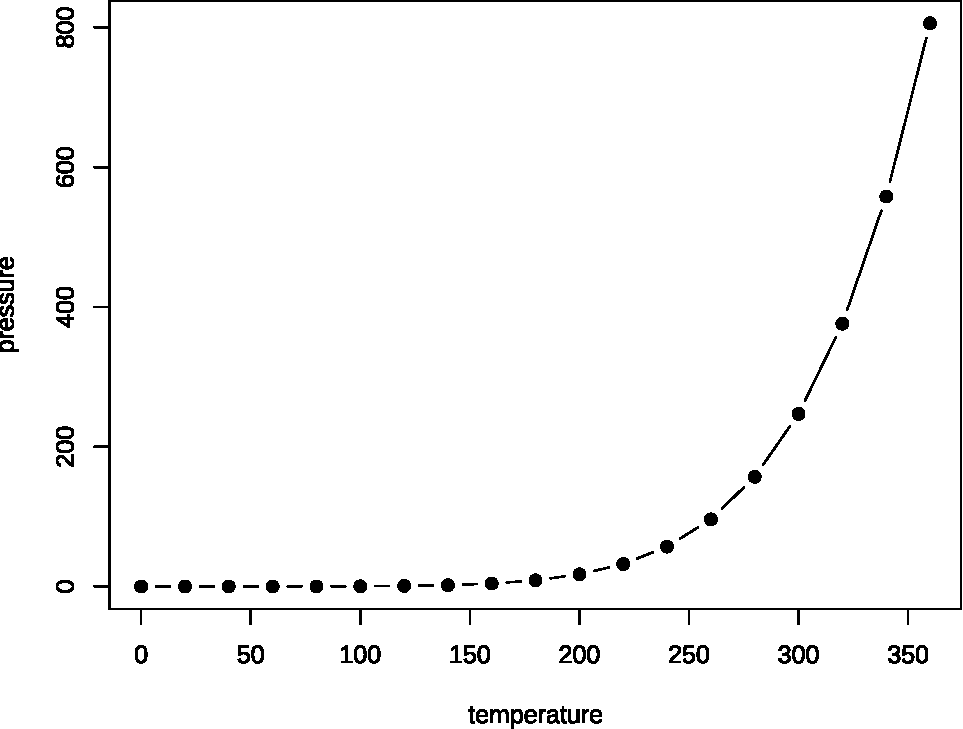
\includegraphics[width=0.8\linewidth]{90-bookdown_files/figure-latex/nice-fig-1} 

}

\caption{Here is a nice figure!}\label{fig:nice-fig}
\end{figure}

Don't miss Table \ref{tab:nice-tab}.

\begin{Shaded}
\begin{Highlighting}[]
\NormalTok{knitr}\SpecialCharTok{::}\FunctionTok{kable}\NormalTok{(}
  \FunctionTok{head}\NormalTok{(pressure, }\DecValTok{10}\NormalTok{), }\AttributeTok{caption =} \StringTok{\textquotesingle{}Here is a nice table!\textquotesingle{}}\NormalTok{,}
  \AttributeTok{booktabs =} \ConstantTok{TRUE}
\NormalTok{)}
\end{Highlighting}
\end{Shaded}

\begin{table}

\caption{\label{tab:nice-tab}Here is a nice table!}
\centering
\begin{tabular}[t]{rr}
\toprule
temperature & pressure\\
\midrule
0 & 0.0002\\
20 & 0.0012\\
40 & 0.0060\\
60 & 0.0300\\
80 & 0.0900\\
\addlinespace
100 & 0.2700\\
120 & 0.7500\\
140 & 1.8500\\
160 & 4.2000\\
180 & 8.8000\\
\bottomrule
\end{tabular}
\end{table}

\hypertarget{parts}{%
\section{Parts}\label{parts}}

You can add parts to organize one or more book chapters together. Parts can be inserted at the top of an .Rmd file, before the first-level chapter heading in that same file.

Add a numbered part: \texttt{\#\ (PART)\ Act\ one\ \{-\}} (followed by \texttt{\#\ A\ chapter})

Add an unnumbered part: \texttt{\#\ (PART\textbackslash{}*)\ Act\ one\ \{-\}} (followed by \texttt{\#\ A\ chapter})

Add an appendix as a special kind of un-numbered part: \texttt{\#\ (APPENDIX)\ Other\ stuff\ \{-\}} (followed by \texttt{\#\ A\ chapter}). Chapters in an appendix are prepended with letters instead of numbers.

\hypertarget{footnotes-and-citations}{%
\section{Footnotes and citations}\label{footnotes-and-citations}}

\hypertarget{footnotes}{%
\subsection{Footnotes}\label{footnotes}}

Footnotes are put inside the square brackets after a caret \texttt{\^{}{[}{]}}. Like this one \footnote{This is a footnote.}.

\hypertarget{citations}{%
\subsection{Citations}\label{citations}}

Reference items in your bibliography file(s) using \texttt{@key}.

For example, we are using the \textbf{bookdown} package \citep{R-bookdown} (check out the last code chunk in index.Rmd to see how this citation key was added) in this sample book, which was built on top of R Markdown and \textbf{knitr} \citep{xie2015} (this citation was added manually in an external file book.bib). Note that the \texttt{.bib} files need to be listed in the index.Rmd with the YAML \texttt{bibliography} key.

The \texttt{bs4\_book} theme makes footnotes appear inline when you click on them. In this example book, we added \texttt{csl:\ chicago-fullnote-bibliography.csl} to the \texttt{index.Rmd} YAML, and include the \texttt{.csl} file. To download a new style, we recommend: \url{https://www.zotero.org/styles/}

The RStudio Visual Markdown Editor can also make it easier to insert citations: \url{https://rstudio.github.io/visual-markdown-editing/\#/citations}

\hypertarget{blocks}{%
\section{Blocks}\label{blocks}}

\hypertarget{equations}{%
\subsection{Equations}\label{equations}}

Here is an equation.

\begin{equation} 
  f\left(k\right) = \binom{n}{k} p^k\left(1-p\right)^{n-k}
  \label{eq:binom}
\end{equation}

You may refer to using \texttt{\textbackslash{}@ref(eq:binom)}, like see Equation \eqref{eq:binom}.

\hypertarget{theorems-and-proofs}{%
\subsection{Theorems and proofs}\label{theorems-and-proofs}}

Labeled theorems can be referenced in text using \texttt{\textbackslash{}@ref(thm:tri)}, for example, check out this smart theorem \ref{thm:tri}.

\begin{theorem}
\protect\hypertarget{thm:tri}{}\label{thm:tri}For a right triangle, if \(c\) denotes the \emph{length} of the hypotenuse and \(a\) and \(b\) denote the lengths of the \textbf{other} two sides, we have \[a^2 + b^2 = c^2\]
\end{theorem}

Read more here \url{https://bookdown.org/yihui/bookdown/markdown-extensions-by-bookdown.html}.

\hypertarget{callout-blocks}{%
\subsection{Callout blocks}\label{callout-blocks}}

The \texttt{bs4\_book} theme also includes special callout blocks, like this \texttt{.rmdnote}.

You can use \textbf{markdown} inside a block.

\begin{Shaded}
\begin{Highlighting}[]
\FunctionTok{head}\NormalTok{(beaver1, }\AttributeTok{n =} \DecValTok{5}\NormalTok{)}
\CommentTok{\#\textgreater{}   day time  temp activ}
\CommentTok{\#\textgreater{} 1 346  840 36.33     0}
\CommentTok{\#\textgreater{} 2 346  850 36.34     0}
\CommentTok{\#\textgreater{} 3 346  900 36.35     0}
\CommentTok{\#\textgreater{} 4 346  910 36.42     0}
\CommentTok{\#\textgreater{} 5 346  920 36.55     0}
\end{Highlighting}
\end{Shaded}

It is up to the user to define the appearance of these blocks for LaTeX output.

You may also use: \texttt{.rmdcaution}, \texttt{.rmdimportant}, \texttt{.rmdtip}, or \texttt{.rmdwarning} as the block name.

The R Markdown Cookbook provides more help on how to use custom blocks to design your own callouts: \url{https://bookdown.org/yihui/rmarkdown-cookbook/custom-blocks.html}

\hypertarget{sharing-your-book}{%
\section{Sharing your book}\label{sharing-your-book}}

\hypertarget{publishing}{%
\subsection{Publishing}\label{publishing}}

HTML books can be published online, see: \url{https://bookdown.org/yihui/bookdown/publishing.html}

\hypertarget{pages}{%
\subsection{404 pages}\label{pages}}

By default, users will be directed to a 404 page if they try to access a webpage that cannot be found. If you'd like to customize your 404 page instead of using the default, you may add either a \texttt{\_404.Rmd} or \texttt{\_404.md} file to your project root and use code and/or Markdown syntax.

\hypertarget{metadata-for-sharing}{%
\subsection{Metadata for sharing}\label{metadata-for-sharing}}

Bookdown HTML books will provide HTML metadata for social sharing on platforms like Twitter, Facebook, and LinkedIn, using information you provide in the \texttt{index.Rmd} YAML. To setup, set the \texttt{url} for your book and the path to your \texttt{cover-image} file. Your book's \texttt{title} and \texttt{description} are also used.

This \texttt{bs4\_book} provides enhanced metadata for social sharing, so that each chapter shared will have a unique description, auto-generated based on the content.

Specify your book's source repository on GitHub as the \texttt{repo} in the \texttt{\_output.yml} file, which allows users to view each chapter's source file or suggest an edit. Read more about the features of this output format here:

\url{https://pkgs.rstudio.com/bookdown/reference/bs4_book.html}

Or use:

\begin{Shaded}
\begin{Highlighting}[]
\NormalTok{?bookdown}\SpecialCharTok{::}\NormalTok{bs4\_book}
\end{Highlighting}
\end{Shaded}

\hypertarget{todo-list}{%
\chapter{To Do リスト}\label{todo-list}}

この文書について

\begin{enumerate}
\def\labelenumi{\arabic{enumi}.}
\tightlist
\item
  はじめに
\end{enumerate}

\begin{itemize}
\tightlist
\item
  1.1 データサイエンスとは

  \begin{itemize}
  \tightlist
  \item
    1.1.1 なぜ、データサイエンスが最近注目されているのか
  \item
    1.1.2 なぜ、一人ひとりが、データサイエンスを、学ぶ必要があるのでしょうか
  \item
    1.1.3 AI の活用
  \end{itemize}
\item
  1.2 「データサイエンスを始めましょう」の特徴

  \begin{itemize}
  \tightlist
  \item
    1.2.1 学習者として想定しているのは
  \item
    1.2.2 オープン・パブリックデータの活用
  \item
    1.2.3 世界のデータをみること
  \item
    1.2.4 目標としていること
  \end{itemize}
\item
  1.3 学習方法について
\item
  1.4 参考
\end{itemize}

\begin{enumerate}
\def\labelenumi{\arabic{enumi}.}
\setcounter{enumi}{1}
\tightlist
\item
  学ぶ内容 
\end{enumerate}

\begin{itemize}
\tightlist
\item
  2.1 データサイエンス入門
\item
  2.2 第一部 パブリックデータ
\item
  2.3 第二部 基本
\item
  2.4 第三部 国際機関などのデータの活用
\item
  2.5 第四部 探索的データ分析 Exploratory Data Analysis
\item
  2.6 第五部 分析例
\item
  2.7 付録
\end{itemize}

\begin{enumerate}
\def\labelenumi{\arabic{enumi}.}
\setcounter{enumi}{2}
\tightlist
\item
  はじめてのデータサイエンス
\end{enumerate}

\begin{itemize}
\tightlist
\item
  3.1 データサイエンスの実際
\item
  3.2 R のパッケージを活用

  \begin{itemize}
  \tightlist
  \item
    3.2.1 準備 Setup
  \item
    3.2.2 データ取得 Import data
  \item
    3.2.3 データ構造の確認
  \item
    3.2.4 必要に応じて整形 Transform data
  \item
    3.2.5 視覚化 data visualization
  \item
    3.2.6 データの理解 Understand data
  \item
    3.2.7 さまざまな視覚化
  \end{itemize}
\item
  3.3 練習
\item
  3.4 プロジェクト
\item
  3.5 まとめ
\end{itemize}

\begin{enumerate}
\def\labelenumi{\arabic{enumi}.}
\setcounter{enumi}{3}
\tightlist
\item
  世界開発指標
\end{enumerate}

\begin{itemize}
\tightlist
\item
  4.1 世界銀行(World Bank)

  \begin{itemize}
  \tightlist
  \item
    4.1.1 世界銀行オープンデータ
  \item
    4.1.2 データカタログ
  \item
    4.1.3 世界開発指標(WDI)
  \item
    4.1.4 オープンデータの定義(Open Data Defined)
  \end{itemize}
\item
  4.2 世界開発指標(WDI)

  \begin{itemize}
  \tightlist
  \item
    4.2.1 世界のさまざまな課題
  \item
    4.2.2 ダッシュボード・データの取得・データコード
  \end{itemize}
\item
  4.3 世界銀行以外の国際機関のパブリックデータ
\item
  4.4 持続的開発目標(SDGs) データ
\item
  4.5 課題
\end{itemize}

PART I PUBLIC DATA

\begin{enumerate}
\def\labelenumi{\arabic{enumi}.}
\setcounter{enumi}{10}
\tightlist
\item
  Public Data
\end{enumerate}

\begin{itemize}
\tightlist
\item
  5.1 オープンデータ

  \begin{itemize}
  \tightlist
  \item
    5.1.1 Open Government Data Toolkit: Open Data Defined
  \end{itemize}
\item
  5.2 日本から世界を見る
\item
  5.3 世界銀行(World Bank)

  \begin{itemize}
  \tightlist
  \item
    5.3.1 世界開発指数(World Development Indicator (WDI))
  \item
    5.3.2 World Bank: WDI - World Development Indicaters
  \item
    5.3.3 世界開発指標(World Development Indicator)
  \item
    5.3.4 例
  \end{itemize}
\item
  5.4 世界のさまざまな課題から見る
\item
  5.5 OECD
\item
  5.6 UN Data
\item
  5.7 Our World in Data
\item
  5.8 Eurostat
\end{itemize}

PART II BASICS

\begin{enumerate}
\def\labelenumi{\arabic{enumi}.}
\setcounter{enumi}{20}
\tightlist
\item
  R Studio で R
\end{enumerate}

\begin{itemize}
\tightlist
\item
  6.1 はじめに
\item
  6.2 R と R Studio
\item
  6.3 R と R Studio のインストール

  \begin{itemize}
  \tightlist
  \item
    6.3.1 R のインストール
  \item
    6.3.2 R Studio の インストール
  \item
    6.3.3 動作確認
  \item
    6.3.4 トラブル・シューティング(1)
  \end{itemize}
\item
  6.4 クラウド - Posit Cloud

  \begin{itemize}
  \tightlist
  \item
    6.4.1 クラウドサービス How to Start Posit Cloud
  \item
    6.4.2 PositCloud Shared Project
  \item
    6.4.3 Posit Primers and Cheat Sheet
  \end{itemize}
\item
  6.5 R のその他の利用方法
\item
  6.5.1 Google colab で R
\item
  6.5.2 CoCalc で R と RMarkdown
\end{itemize}

\begin{enumerate}
\def\labelenumi{\arabic{enumi}.}
\setcounter{enumi}{21}
\tightlist
\item
  R Markdown
\end{enumerate}

\begin{itemize}
\tightlist
\item
  7.1 Reproducible and Literate Programming

  \begin{itemize}
  \tightlist
  \item
    7.1.1 目的、問いなど
  \item
    7.1.2 データについて
  \item
    7.1.3 コードについて
  \item
    7.1.4 グラフについて
  \item
    7.1.5 まとめ:R Markdown の目的
  \end{itemize}
\item
  7.2 準備:パッケージのインストール
\item
  7.3 R Notebook
\item
  7.4 日本語のテンプレート
\item
  7.5 R Markdown いくつかの Output
\item
  7.6 YouTube Video - rmarkdown -7.6.1 RMarkdown で PDF を作成するときの注意
\end{itemize}

\begin{enumerate}
\def\labelenumi{\arabic{enumi}.}
\setcounter{enumi}{22}
\tightlist
\item
  R Basics
\end{enumerate}

\begin{itemize}
\tightlist
\item
  8.1 プロジェクト - Project
\item
  8.2 コンソールで実行 - Run in Console

  \begin{itemize}
  \tightlist
  \item
    8.2.1 最初の四つ
  \item
    8.2.2 アサインメント、ヘルプ
  \item
    8.2.3 おすすめ
  \item
    8.2.4 練習
  \end{itemize}
\item
  8.3 RStudio について

  \begin{itemize}
  \tightlist
  \item
    8.3.1 四つの窓枠とタブ Four Panes and Tabs
  \end{itemize}
\item
  8.4 R Script 実行記録

  \begin{itemize}
  \tightlist
  \item
    8.4.1 R Script の作成
  \item
    8.4.2 R Script による実行
  \item
    8.4.3 練習
  \item
    8.4.4 Tips
  \end{itemize}
\item
  8.5 パッケージ - Packages

  \begin{itemize}
  \tightlist
  \item
    8.5.1 パッケージのインストール
  \item
    8.5.2 備考
  \end{itemize}
\item
  8.6 練習問題 Posit Primers

  \begin{itemize}
  \tightlist
  \item
    8.6.1 最初の演習 The Basics -- r4ds: Explore, I
  \end{itemize}
\item
  8.7 参考文献 References
\item
  8.8 YouTube Video - getstarted
\end{itemize}

PART III INSTITUTIONAL DATA

\begin{enumerate}
\def\labelenumi{\arabic{enumi}.}
\setcounter{enumi}{30}
\tightlist
\item
  World Bank
\end{enumerate}

\begin{itemize}
\tightlist
\item
  9.1 World Development Indicator (WDI)

  \begin{itemize}
  \tightlist
  \item
    9.1.1 指標 Indicators (WDI)
  \item
    9.1.2 指標 WDI (World Development Indicators)
  \item
    9.1.3 指標 のコード、WDI code を探してみよう
  \item
    9.1.4 指標 WDIの例
  \item
    9.1.5 練習 1. - 調べてみたい WDI 指標とそのコード
  \end{itemize}
\item
  9.2 WDI パッケージ

  \begin{itemize}
  \tightlist
  \item
    9.2.1 指標 WDI 検索
  \item
    9.2.2 指標 WDI データのダウンロード
  \end{itemize}
\item
  9.3 可視化 Visualization

  \begin{itemize}
  \tightlist
  \item
    9.3.1 グラフ 1
  \item
    9.3.2 グラフ 2
  \item
    9.3.3 テンプレート Templates -9.4 課題 Assignment
  \end{itemize}
\end{itemize}

PART IV EDA

\begin{enumerate}
\def\labelenumi{\arabic{enumi}.}
\setcounter{enumi}{40}
\tightlist
\item
  探索的データ解析
\end{enumerate}

\begin{itemize}
\tightlist
\item
  10.1 探索的データ解析 (EDA)とは
\item
  10.2 探索的データ解析 (EDA) の一例

  \begin{itemize}
  \tightlist
  \item
    10.2.1 データの取得と読み込み - Data Import
  \item
    10.2.2 データ変形・整形 - Data Transformation
  \item
    10.2.3 可視化 Data Visualization
  \item
    10.2.4 データモデリング Data Modeling
  \end{itemize}
\end{itemize}

PART V EXAMPLES

\begin{enumerate}
\def\labelenumi{\arabic{enumi}.}
\setcounter{enumi}{50}
\tightlist
\item
  Example 1
\end{enumerate}

APPENDIX

\begin{enumerate}
\def\labelenumi{\arabic{enumi}.}
\setcounter{enumi}{80}
\tightlist
\item
  日本語の扱いについて
\end{enumerate}

\begin{itemize}
\tightlist
\item
  A.1 日本語・中国語・韓国語

  \begin{itemize}
  \tightlist
  \item
    A.1.1 パッケージをロード
  \end{itemize}
\item
  A.2 Base R でタイトルに日本語
\item
  A.3 列名や、データに日本語
\item
  A.4 kable で表示
\item
  A.5 ggplot でグラフを作成
\item
  A.6 備考:
\item
  A.7 参考:日本語の表示について

  \begin{itemize}
  \tightlist
  \item
    A.7.1 データファイルの読み込み
  \item
    A.7.2 図の中のテキスト
  \item
    A.7.3 R Markdown の出力
  \item
    A.7.4 bookdown
  \item
    A.7.5 参考としたもの
  \end{itemize}
\end{itemize}

\begin{enumerate}
\def\labelenumi{\arabic{enumi}.}
\setcounter{enumi}{84}
\tightlist
\item
  IT ツール
\end{enumerate}

\begin{itemize}
\tightlist
\item
  B.1 Git と GitHub

  \begin{itemize}
  \tightlist
  \item
    B.1.1 概要
  \item
    B.1.2 はじめかた
  \item
    B.1.3 GitHub にあるリモート・リポジトリ(Remote Repo)から始める場合
  \item
    B.1.4 自分のコンピュータのリポジトリ(Local Repo)から始める場合
  \item
    B.1.5 GitHub Pages について
  \item
    B.1.6 Bookdown パッケージによる、電子書籍の執筆
  \item
    B.1.7 大きなファイルに関すること
  \item
    B.1.8 複数のコンピュータから利用する方法
  \item
    B.1.9 複数のアカウントを一つのコンピュータから利用する方法
  \item
    B.1.10 共同作業をする場合
  \item
    B.1.11 参考にしたサイト
  \end{itemize}
\end{itemize}

\begin{enumerate}
\def\labelenumi{\arabic{enumi}.}
\setcounter{enumi}{89}
\tightlist
\item
  Bookdown
\item
  To do list
\end{enumerate}

\renewcommand\bibname{参考文献}
  \bibliography{book.bib,packages.bib}

\end{document}
